% file thesis.tex
% Archivo thesis.tex
% Documento maestro que incluye todos los paquetes necesarios para el documento
% principal.

% Documento obtenido por un sinfin de iteraciones de administradores del LDC
% Estructura actual hecha por:
% Jairo Lopez <jairo@ldc.usb.ve>
% Actualizado ligeramente por:
% Alexander Tough 

\documentclass[oneside,11pt,letterpaper]{report}
\tolerance=1000  
\hbadness=10000  
\raggedbottom

% Paquetes para manejar graficos
\usepackage{epsf}
\usepackage[pdftex]{graphicx}
\usepackage{epstopdf}
\usepackage{epsfig}
% Simbolos matematicos
\usepackage{latexsym,amssymb}
% Paquetes para presentar una tesis decente.
\usepackage{setspace,cite} % Doble espacio para texto, espacio singular para
                           % los caption y pie de pagina
\usepackage{verbatim}

% Paquetes no utilizados para citas
%\usepackage{mcite} 
%\usepackage{draft} 

\usepackage{wrapfig}
\usepackage{alltt}

\usepackage{tikz}
\usetikzlibrary{positioning,shapes}

% Acentos 
\usepackage[spanish,activeacute,es-tabla]{babel}
\usepackage[spanish]{translator}
\usepackage[utf8]{inputenc}
\usepackage{color, xcolor, colortbl}
\usepackage{multirow}
\usepackage{subfig}
\usepackage{float}
\usepackage[OT1]{fontenc}
\usepackage{tocbibind}
\usepackage{anysize}
\usepackage{listings}
\usepackage{morefloats}
\usepackage[section,verbose]{placeins}
\usepackage{pdflscape}

\renewcommand{\thesubfigure}{\thefigure.\arabic{subfigure}}

% Para poder tener texto asiatico
%\usepackage{CJK}

% Opciones para los glosarios
\usepackage[style=altlist,toc,numberline,acronym]{glossaries}
\usepackage{url}
\usepackage{amsthm}
\usepackage{amsmath}
\usepackage{fancyhdr} % Necesario para los encabezados
\usepackage{fancyvrb}
\usepackage{makeidx} % En caso de necesitar indices.
\makeindex  % Necesitado para los indices

% Definiciones para definicions, teoremas y lemas
\theoremstyle{definition} \newtheorem{definicion}{Definici\'{o}n}
\theoremstyle{plain} \newtheorem{teorema}{Teorema}
\theoremstyle{plain} \newtheorem{lema}{Lema}

% Para la creacion de los pdfs
\usepackage{hyperref}

% Para resolver el lio del Unicode para la informacion de los PDFs
% En pdftitle coloca el nombre de su proyecto de grado/pasantia.
% En pdfauthor coloca su nombre.
\hypersetup{
    pdftitle = {Clustering de datos numéricos por medio de algoritmos basados en población e inteligencia colectiva},
    pdfauthor= {Alexander De Sousa y Federico Ponte},
    colorlinks,
    citecolor=black,
    filecolor=black,
    linkcolor=black,
    urlcolor=black,
    backref,
    pdftex
}

\lstset{
   language=C,
   basicstyle=\footnotesize,
   keywordstyle=\textbf,
   showstringspaces=false,
   numbers=left,
   numberstyle=\footnotesize,
   mathescape=true,
   escapechar={\%},
   frame=bottomline,
   captionpos=t,
   morekeywords={Mientras, Si, Sino, Para, Fin, FinSi, FinPara, FinMientras},
   commentstyle={\color{darkgrey}},
   literate={á}{{\'a}}1
            {é}{{\'e}}1
            {í}{{\'i}}1
            {ó}{{\'o}}1
            {ú}{{\'u}}1
            {ñ}{{\~n}}1
}

\usepackage{tikz}
\usetikzlibrary{positioning,shapes}
\usepackage{lmodern}
\usepackage{amsfonts}
\definecolor{darkgrey}{rgb}{0.4,0.4,0.4}
\usepackage{caption}
\DeclareCaptionFont{white}{\color{white}}
\DeclareCaptionFormat{listing}{\colorbox{gray}{\parbox{\textwidth}{#1#2#3}}}
\captionsetup[lstlisting]{format=listing,labelfont=white,textfont=white}
\renewcommand{\lstlistingname}{Pseudo-código}
\renewcommand{\lstlistlistingname}{Índice de pseudo-códigos}


% Crea el glosario
%\makeglossaries

% Incluye el glosario
%\input{glossary.tex}

% Para crear la hoja escaneada de las firmas
\usepackage[absolute]{textpos}

% Pone los nombres y las opciones para mostrar los codigos fuentes
%\usepackage[ruled,vlined,linesnumbered, algochapter]{algorithm2e}    % Algoritmos
%\usepackage{algorithmic}    % Algoritmos

% Dimensiones de la pagina
\setlength{\headheight}{15pt}
\marginsize{2.8cm}{1.5cm}{1.2cm}{1.2cm}
%\marginsize{2.5cm}{1.8cm}{1.2cm}{1.2cm}

% Se pueden omitir para que no compile ciertos capitulos.
%\includeonly{header, intro, ssimilar, herramienta, resultados, conclusiones}

%%%%%%%%%%%%%%%%%%%%%%%%%%%%%%%%%%%%%%%%%%%%%%%%%%%%%%%%%%%%%%%%%%%%%%%%%%%
%%%%%%%%%%%%%%%%      end of preamble and start of document     %%%%%%%%%%%
%%%%%%%%%%%%%%%%%%%%%%%%%%%%%%%%%%%%%%%%%%%%%%%%%%%%%%%%%%%%%%%%%%%%%%%%%%%
\begin{document}
\pagenumbering{roman}
\setcounter{page}{2}
% Pagina de titulo
\setcounter{page}{3}
% Pagina de titulo
\begin{titlepage}
\begin{center}

% Upper part (aqui ya esta incluido el logo de la USB).
\includegraphics[scale=0.5,type=png,ext=.png,read=.png]{figures/cebolla} \\

% Encabezado
\textsc {\large UNIVERSIDAD SIM'ON BOL'IVAR} \\
\textsc{\bfseries DECANATO DE ESTUDIOS PROFESIONALES\\
COORDINACI'ON DE INGENIER'IA DE LA COMPUTACI'ON}

\bigskip
\bigskip
\bigskip
\bigskip
\bigskip
\bigskip
\bigskip
\bigskip
\bigskip

% Title/Titulo
% Aqui ponga el nombre de su proyecto de grado/pasantia larga
\textsc{\bfseries Clustering de datos numericos por medio de algoritmos basados en poblacion e inteligencia colectiva}

\bigskip
\bigskip
\bigskip
\bigskip
\bigskip

% Author and supervisor/Autor y tutor
\begin{minipage}{\textwidth}
\centering
Por: \\
Alexander De Sousa\\
Federico Ponte \\

\bigskip
\bigskip
\bigskip

Realizado con la asesor'ia de: \\
Emely Arra\'iz
\end{minipage}

\bigskip
\bigskip
\bigskip
\bigskip
\bigskip
\bigskip
\bigskip
\bigskip
\bigskip

% Bottom half
{PROYECTO DE GRADO \\ Presentado ante la Ilustre Universidad Sim'on Bol'ivar \\
como requisito parcial para optar al t'itulo de \\ Ingeniero en Computaci'on} \\

\bigskip
\bigskip
\vfill

% Date/Fecha 
{\large \bfseries Sartenejas, FECHA (MES de A\~NO)}

\end{center}
\end{titlepage}


% Pagina de acta final (vacio)
% Pagina del acta final
\begin{titlepage}
\begin{center}

% Upper part
\includegraphics[scale=0.5,type=png,ext=.png,read=.png]{figures/cebolla} \\

\textsc {\large UNIVERSIDAD SIMÓN BOLÍVAR} \\
\textsc{DECANATO DE ESTUDIOS PROFESIONALES\\
COORDINACIÓN DE INGENIERÍA DE LA COMPUTACIÓN}

\bigskip
\bigskip
\bigskip
\bigskip
\bigskip
\bigskip

% Title
\textsc{ACTA FINAL PROYECTO DE GRADO}

\bigskip
\bigskip

% Aqui coloca el nombre de su proyecto de grado/pasantia larga.
\textsc{\bfseries Clustering de Datos Numéricos por medio de Algoritmos Basados en Población e Inteligencia Colectiva}

\bigskip
\bigskip
\bigskip
\bigskip

\begin{minipage}{\textwidth}
\centering
Presentado por: \\
% Aqui coloca su nombre.
\textsc{\bfseries Alexander José De Sousa De Andrade} \\
\textsc{\bfseries Federico Ignacio Ponte Betancourt} \\

\bigskip
\bigskip
\bigskip
\bigskip

\includegraphics[width=0.8\textwidth]{figures/firmas.jpg}\\

\end{minipage}

\bigskip
\bigskip
\vfill

% Date/Fecha
{\large \bfseries Sartenejas, Septiembre de 2011}

\end{center}
\end{titlepage}


\setcounter{secnumdepth}{3}
\setcounter{tocdepth}{4}

% Define encabezado numeros romanos y como se separan los captiulos y las
% secciones
\addtolength{\headheight}{3pt}
%\pagenumbering{roman}
\pagestyle{fancyplain}

\renewcommand{\chaptermark}[1]{\markboth{\chaptername\ \thechapter:\,\ #1}{}}
\renewcommand{\sectionmark}[1]{\markright{\thesection\,\ #1}}

\onehalfspacing

\lhead{}
\chead{}
\rhead{}
\renewcommand{\headrulewidth}{0.0pt}
\lfoot{}
\cfoot{\fancyplain{}{\thepage}}
\rfoot{}


% Pagina de resumen
\vspace{5 mm}

\setcounter{page}{4}
\begin{center}
	{\bf Resumen}
\end{center}

\vspace{5 mm}

La agrupación de datos (\emph{data clustering}) es el proceso de particionar una
colección de datos en conjuntos de clases significativas, llamadas \emph{clusters},
donde los objetos de una clase comparten ca\-rac\-te\-rís\-ti\-cas comunes. En este trabajo,
se presenta un estudio comparativo de cinco metaheurísticas basadas en población
e inteligencia colectiva (\emph{algoritmo genético}, \emph{optimizador de enjambre
de partículas}, \emph{evolución diferencial}, \emph{algoritmo de abeja} y
\emph{algoritmo de clustering de hormigas}) para resolver el problema de \emph{data
clustering} en calidad de soluciones finales. Los datos usados para el estudio son
de tipo numérico, comúnmente utilizados en la literatura afín. Del estudio se
llega a la conclusión que para resolver el problema de \emph{clustering} de datos
numéricos se deben utilizar el \emph{algoritmo genético} o el \emph{algoritmo de
abeja}, ambos hibridados con la heurística \emph{K-means} como método de mejoramiento
de las soluciones finales.

\newpage



% Pagina de dedicatoria (opcional)
\setcounter{page}{5}

\pdfbookmark[0]{Dedicatoria}{dedication} % Sets a PDF bookmark for the dedication
\vspace*{8cm} 
\begin{center} 
\large A nuestras familias y amigos.
\end{center}
\newpage


% Pagina de agradecimientos (opcional)
\setcounter{page}{6}

\chapter*{Agradecimientos
\markboth{Agradecimientos}{Agradecimientos}}
A todas las personas que aportaron su granito de arena en la realización de este
proyecto de grado, en especial, nuestra tutora.


% Crea la tabla de contenidos
\tableofcontents

% Crea la lista de cuadros
\listoftables

% Crea la lista de figuras
\listoffigures

% Crea la lista de codigos fuentes
\lstlistoflistings
\addcontentsline{toc}{chapter}{\'Indice de pseudo-c\'odigos}

\clearpage

% Define encabezado en numeros arabicos  
\pagenumbering{arabic}
\setcounter{page}{1}

\fancyhf{} % Redefine el encabezado 
\lhead{}
\chead{}
\rhead{\fancyplain{}{\thepage}}
\renewcommand{\headrulewidth}{0.0pt}
\lfoot{}
\cfoot{}
\rfoot{}

\onehalfspacing


% Incluye los archivos deseados - El contenido de
% su proyecto de grado/pasantia larga.
\phantomsection
\addcontentsline{toc}{chapter}{Introducción}
% Titulo de la introduccion.
\begin{center}
	{\bf Introducción} 
\label{chap:intro}
\end{center}

    Los humanos tienen la habilidad innata de relacionar los objetos que los
rodean con la información aprendida previamente. Esta habilidad les permite 
reconocer y clasificar de forma intuitiva di\-fe\-ren\-tes tipos de objetos. Sin
embargo, hacer que una computadora clasifique y reconozca objetos en grupos es
una tarea difícil.

    A medida que aumenta la cantidad de información con la que tienen que lidiar
los seres humanos, también crece la necesidad de poder procesarla y clasificarla
de manera automática. Por lo tanto, este problema ha sido ampliamente abordado
por investigadores en las área de estadística, inteligencia de negocios,
inteligencia artificial, etc\cite{SwAjAm2009}. Un componente fundamental
del área de inteligencia artificial es el reconocimiento de patrones donde uno de
sus objetivos es el de clasificar objetos en diferentes categorías o clases. Cuando
esta clasificación no es supervisada por un ser humano, se llama \emph{data
clustering}.

    El problema de \emph{Data clustering} es la clasificación no supervisada de
un conjunto de datos en grupos similares. Los datos pertenecientes a un grupo
(\emph{cluster}) tienen más similitudes entre sí, que con los datos pertenecientes
a otros grupos \cite{GaChJi2007}. Brucker en \cite{Br1978} demostró que el
problema es \emph{NP-hard} cuando el número de clusters excede a 3.

    Entre las aplicaciones de la resolución del problema de \emph{data clustering}
(minería de datos, segmentación de clientes, recuperación de documentos, etc.),
destaca el procesamiento de imágenes \cite{GaChJi2007}. Su importancia radica en
que el resultado de hacer \emph{data clustering} a una imagen puede ser usado
como entrada para una red neuronal de reconocimiento de objetos o de ayuda para
encontrar regiones de interés en imágenes médicas \cite{GaChJi2007}.

    Las metaheurísticas basadas en población e inteligencia colectiva
generalmente son apropiadas para resolver problemas \emph{NP-hard}, incluyendo
el problema de \emph{data clustering}, debido a que pueden evitar quedar atrapados
en soluciones óptimas locales y, normalmente, encuentran la solución óptima global
\cite{PSO_0}. Las metaheurísticas más conocidas y prometedoras son los algoritmos
genético \cite{DoGeGr2007}, de abeja\cite{BEE_0} y de hormiga\cite{Ant_0}\cite{OuBa2007},
el optimizador de enjambre de partículas \cite{PSO_0} y la evolución diferencial
\cite{SwAjAm2008}. Todas estas metaheurísticas funcionan con un grupo de individuos
que se mueven en un espacio de soluciones factibles del problema. La forma en
que se producen estos movimientos depende de cada algoritmo.

    El objetivo de este proyecto de grado consiste en implementar un grupo de
metaheurísticas (los algoritmos \emph{genético}\cite{DoGeGr2007}, \emph{de abeja}
\cite{BEE_0} y \emph{de hormiga} \cite{OuBa2007}, la \emph{evolución diferencial}
\cite{SwAjAm2008} y el \emph{optimizador de enjambre de partículas}\cite{PSO_0})
y el algoritmo determinista \emph{K-means} \cite{GePo2010}, con el propósito de
analizar cual de ellas presenta el mejor desempeño en la resolución del problema
de \emph{data clustering}. Para ello se ejecutaron las diferentes metaheurísticas
con un conjunto de archivos numéricos populares (que pueden representar imágenes
o no) en la literatura afín. Cada metaheurística tuvo que pasar por un proceso de
entonación de parámetros, utilizando un esquema de trabajo basado en el diseño
de experimentos. Finalmente, se realizó un análisis comparativo de los resultados
de las ejecuciones que arrojó la selección de dos metaheurísticas particulares:
algoritmos \emph{genético} y \emph{abeja}. Estas dos son las recomendadas como
buenas para la resolución del problema de \emph{data clustering} tratado en este
trabajo.

    Este documento se encuentra organizado de la siguiente manera: en el primer
capítulo, se tratan los algoritmos de optimización tradicionales y no tradicionales,
además, se describen de manera general las metaheurística implementadas. En el
segundo capítulo, se define el problema de \emph{data clustering} y los índices
de validez usados para la comparación de las metaheurísticas. En el tercer
capítulo, se describen los detalles de implementación de cada metaheurística
implementada. En el cuarto capítulo, se muestran los resultados de los algoritmos
implementados. En el quinto capítulo, se realiza un análisis comparativo de los
resultados obtenidos. Finalmente, en el sexto capítulo, se presentan las
conclusiones y las recomendaciones para trabajos de investigación futuros.

% Contenido de la introduccion.
\begin{comment}
\label{sect:motivacion}

\emph{Data clustering} es la clasificación no supervisada de un conjunto de datos
en grupos similares. Los datos pertenecientes a un grupo tienen más similitudes
entre sí, que con los datos pertenecientes a otros grupos \cite{GaChJi2007}.
Brucker en \cite{Br1978} demostró que el problema es \emph{NP-hard} cuando el
número de clusters excede a 3.

Este problema tiene las siguientes particularidades\cite{SwAjAm2009}:

\begin{itemize}

\item Es necesario definir un criterio de agrupación sobre el conjunto de datos
a particionar. Dependiendo del criterio escogido, los clusters construidos sobre
el mismo conjunto de datos pueden ser diferentes, tanto en número como en
elementos constitutivos. Veamos un ejemplo:\\

Considere los siguientes animales: oveja, perro, gato (mamíferos); gorrión,
gaviota (aves); víbora, lagarto (reptiles); pez de colores, salmonete, tiburón
azul (peces) y rana (anfibio). Si elegimos como criterio la manera como se
reproducen, la oveja, el perro, el gato y el tiburón azul (vivíparos) van a ser
asignados al mismo cluster, mientras que el resto van a ser asignados a un
segundo cluster (figura \subref{fig:ejemplo1}). Por otro lado, si el criterio es el
ambiente donde viven, la oveja, el perro, el gato, el gorrión, la gaviota, la
víbora y el lagarto van a formar un cluster (terrestres), el pez de colores, el
salmonete y el tiburón azul van a formar otro (acuáticos), y un tercero que va a
contener a la rana (anfibios) (figura \subref{fig:ejemplo2}).

\begin{figure}[hbt!]
  \centering
  \subfloat[\emph{Forma cómo se reproducen}]{\label{fig:ejemplo1}\includegraphics[width=0.5\textwidth]{figures/ejemplo1.png}}\\
  \subfloat[\emph{Ambiente donde viven}]{\label{fig:ejemplo2}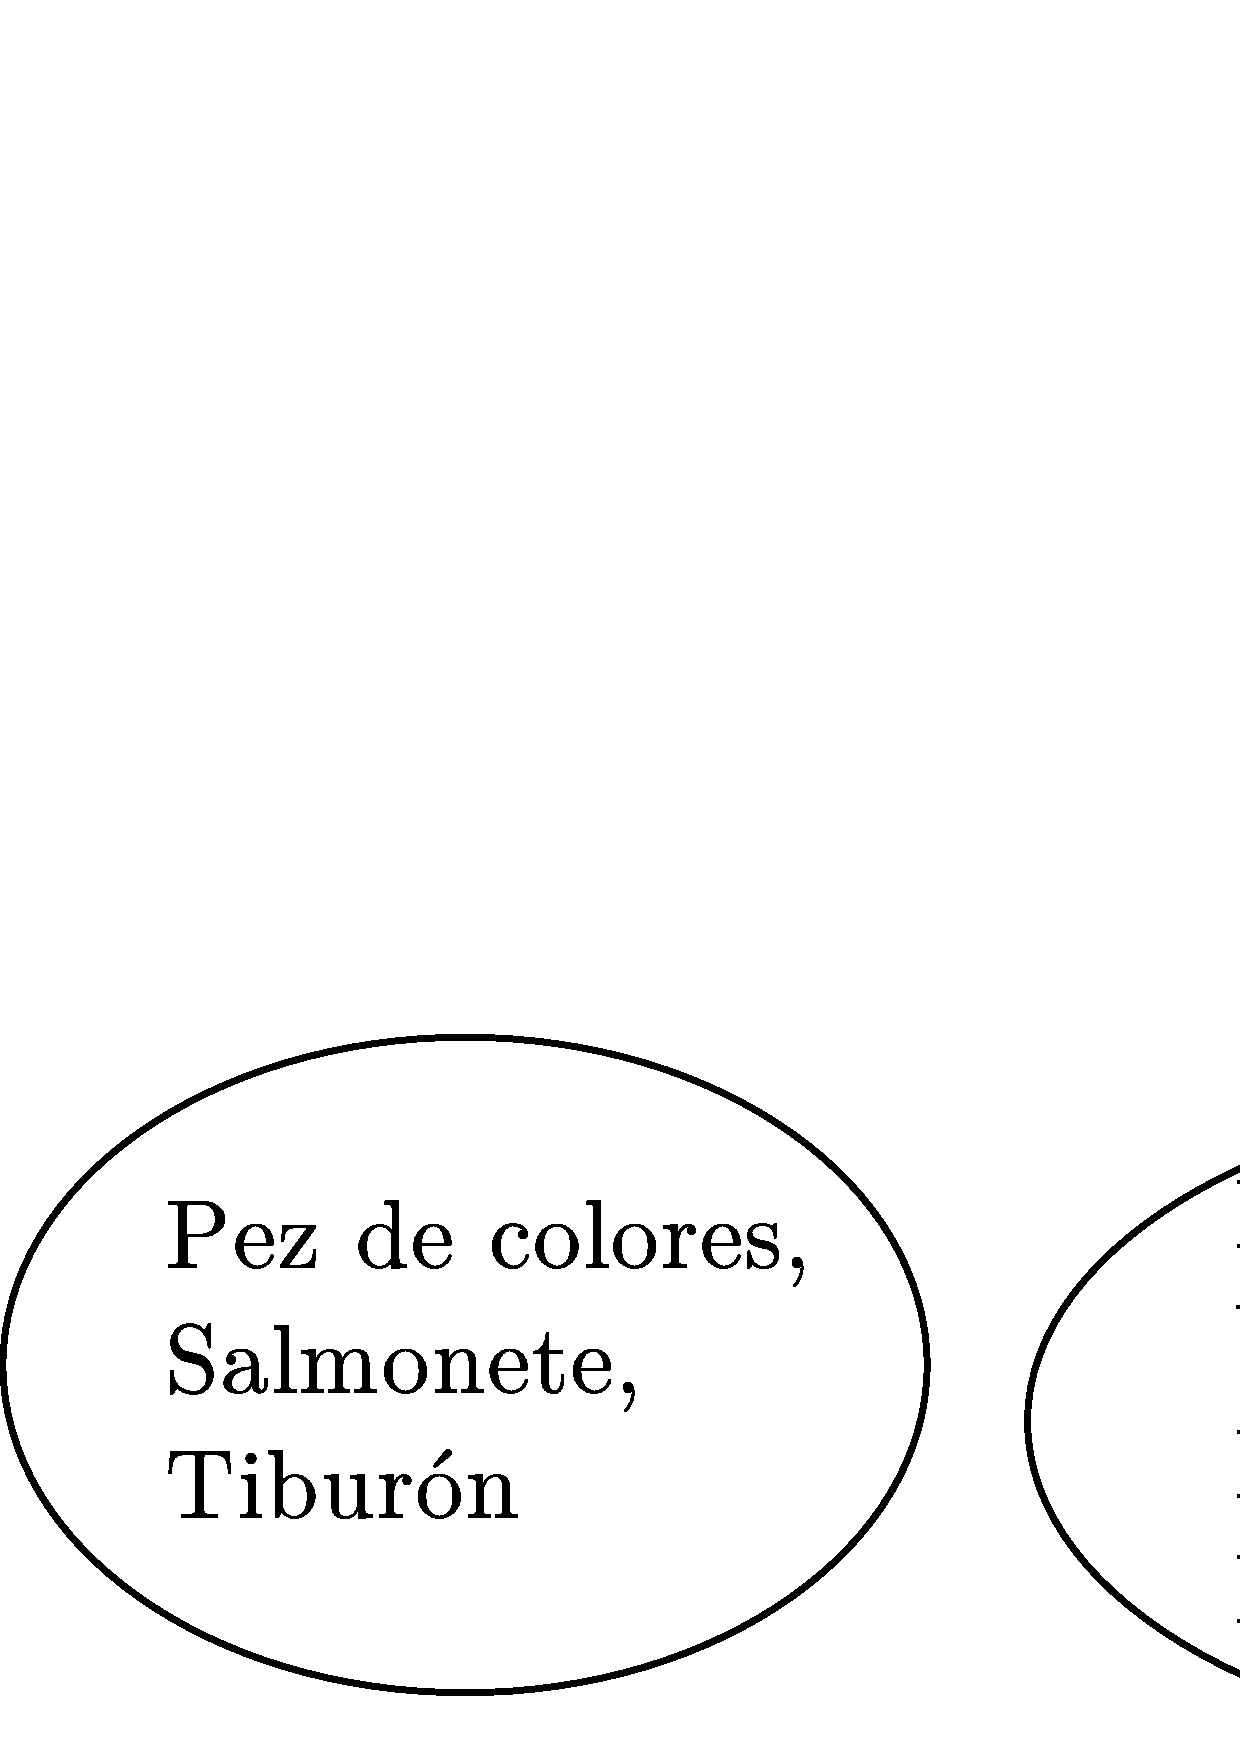
\includegraphics[width=0.5\textwidth]{figures/ejemplo2.png}}
  \caption{Clustering de acuerdo a diferentes criterios}
  \label{fig:ejemplos}
\end{figure}

%Se puede ver que gracias a la falta de un criterio universal para el clustering,
% \'esta es muy subjetiva en muchos casos.
\item Es importante entender la diferencia
entre clustering (aprendizaje no supervisado) y clasificación supervisada. 
En esta última, se tiene una colección de patrones etiquetados
(pre-clasificados) y se quiere etiquetar un nuevo patrón encontrado.
Típicamente, los patrones ya etiquetados son usados para obtener
las descripciones de las clases, que a su vez se utilizan para etiquetar el
nuevo patrón.
%Se puede ver desde el punto de vista de aprendizaje autom\'atico, donde los clusters
%correponden a patrones escondidos en los datos, la b\'usqueda de clusters 
%es una especie de aprendizaje no supervisado. 
En el caso de clustering, el problema consiste en agrupar una colección de
patrones no etiquetados en grupos significativos. En este sentido, las etiquetas
se asocian con los clusters.

\item Se espera que un algoritmo de clustering descubra el agrupamiento natural
que existe en conjunto de patrones o datos. Cada patrón puede ser identificado
como un punto en un hiper-espacio, llamado espacio de características. La entrada
del algoritmo es un conjunto de puntos del hiper-espacio característico. Un
algoritmo ideal de clustering debe tener como salida, la etiqueta de cada
patrón, es decir, el grupo al cual pertenece.
\end{itemize}

\pagebreak
	Este problema ha sido abordado por diversos campos del conocimiento como la
estadística (análisis multivariado), teoría de grafos, computación evolutiva,
redes neuronales, entre otros\cite{SwAjAm2009}. Algunas de sus aplicaciones son
la minería de datos, segmentaciones de clientes, recuperación de documentos y
procesamiento de imágenes \cite{GaChJi2007}. En especial, llama la atención el
último campo mencionado. El procesamiento de imágenes es muy útil para los
humanos. Su importancia radica en que, el resultado de hacer clustering a una
imagen, puede ser usado como la entrada para un modelo basado en sistemas de
reconocimiento de objetos. También, en el área médica, puede ayudar a encontrar
regiones en las imágenes que sean de interés.

%Actualmente existe una amplia investigaci\'on sobre la aplicaci\'on de distintas metaheur\'isticas para
%resolver diversos problemas optimizaci\'on. La idea es encontrar en un tiempo
%razonable la respuesta \'optima o una lo m\'as cercana a ella. Muchos cient\'ificos han empezado a inspirarse en la naturaleza.
%Una profunda obsevaci\'on en la relaci\'on subyacente 
%entre la naturaleza y optimizaci\'on ha llevado al desarrollo de nuevos paradigmas
%para lograr este objetivo\cite{SwAjAm2009}. De ac\'a surgen las basadas en poblaci\'on e inteligencia
%colectiva.
Actualmente existe una amplia investigación sobre la aplicación de distintas
metaheurísticas para resolver diversos problemas optimización. La idea es
encontrar en un tiempo razonable la respuesta óptima o cercana a ella. Muchos
científicos, inspirándose en la naturaleza, han encontrado una relación
subyacente entre ésta y la optimización lo cual ha propiciado el desarrollo de
nuevos paradigmas para lograr este objetivo\cite{SwAjAm2009}. Así que surgen las
metaheurísticas basadas en población e inteligencia colectiva.

%Las m\'as conocidas y prometedoras son el algoritmo g\'enetico, la abeja, la evoluci\'on diferencial(DE), la hormiga
%y el optimizador de enjambre de part\'iculas (PSO). Todos constan de un grupo de individuos que van a ir modificandose a trav\'es
%del tiempo. La forma en que se den estos cambios depende de cada algoritmo.
Las metaheurísticas más conocidas y prometedoras son el algoritmo genético, de
abeja y hormiga, el optimizador de enjambre de partículas, la evolución
diferencial. Todas estas metaheurísticas funcionan con un grupo de individuos
(soluciones) que se modifican a lo largo de la ejecución de las mismas. La forma
en que se den estos cambios depende de cada algoritmo.

Para este trabajo, se implementaron siete metaheurísticas y el algoritmo
determinista \emph{K-means} para resolver el problema de \emph{data clustering}
y se realizó un estudio comparativo de sus desempeños.
La entonación de los parámetros de cada metaheurística se realizó utilizando un
esquema de trabajo basado en el diseño de experimentos; adicionalmente, se
intentó utilizar el análisis de varianza para determinar los parámetros que
tienen mayor influencia en el desempeño de cada metaheurísticas y así orientar
el proceso de entonación. El objetivo principal que se busca es identificar las
metaheurísticas que mejor resuelven el problema de clustering de datos numéricos.

Este documento se encuentra organizado de la siguiente manera: en el primer
capítulo, se tratan los algoritmos de optimización tradicionales y no
tradicionales, además se describen de manera general las metaheurística
implementadas. En el segundo capítulo, se define el problema de cluster y los
índices de validez usados para la comparación de las metaheurísticas. En el 
tercer capítulo, se describen los detalles de implementación de cada
metaheurística implementada. En el cuarto capítulo, se realiza un análisis
comparativo de los resultados obtenidos. Finalmente, en el quito capítulo, se
presentan las conclusiones y las recomendaciones para trabajos de investigación
futuros.
\end{comment}

\chapter{Métodos de Optimización} \label{chap:mopt}

El objetivo de la optimización es buscar valores para un conjunto de
parámetros que maximicen o minimicen la función objetivo del problema de modo
que se satisfagan las restricciones del mismo. Una solución factible es una
elección de valores para el conjunto de parámetros que satisfacen todas las
las restricciones del problema. Las soluciones factibles con mejores valores de
función objetivo son llamadas soluciones óptimas.

    Las técnicas de optimización son usadas diariamente para planificación
industrial, administración de recursos, programación de horarios, toma de
decisiones, agrupación no supervisada de datos, etc. Por lo tanto, las técnicas de
optimización son ampliamente usadas en muchos campos como ingeniería, industria,
medicina y negocios. La investigación en el campo de la optimización es bastante
activa y nuevos métodos de optimización son desarrollados regularmente \cite{GO_1}.

    La optimización abarca tanto problemas de maximización como de minimización.
Cualquier problema de maximización puede ser convertido en un problema de
minimización al tomar la inversa de la función objetivo del mismo y
viceversa. En general, un problema de optimización puede ser definido como:

    Sea $S$ el espacio de soluciones y $d$ la dimensión del mismo donde:
\begin{itemize}
    \item $f: S \rightarrow \mathbb{R}$ es la función objetivo de maximización
del problema.
    \item $S \subseteq \mathbb{R}^d$
\end{itemize}
    entonces se debe encontrar $x^* \in S$ tal que:
\begin{itemize}
    \item $f(x^*) \geq f(x), \forall x \in S$ si se desea una función maximizadora.
    \item $f(x^*)^{-1} \leq f(x)^{-1}, \forall x \in S$, si se desea una función
minimizadora.
\end{itemize}

    El valor de $f(x^*)$ (ó $f(x^*)^{-1}$) es llamado óptimo global. La
optimización global es la tarea de encontrar la solución global óptima. En
general, existen soluciones que son localmente óptimas pero no globalmente
óptimas. Por lo tanto los problemas de optimización global son difíciles de
resolver de manera exacta. En el contexto de problemas combinatorios, estos
problemas son frecuentemente NP-hard \cite{GO_2}. Un buen algoritmo de
optimización global encontrará $x^*$ sin importar el punto inicial $x_0 \in S$.

    Algunos ejemplos de problemas de optimización global son \cite{GO_2}:
\begin{itemize}
    \item Problemas combinatorios: donde la función lineal o no-lineal es definida
sobre un conjunto finito, pero bastante grande de soluciones, Por ejemplo,
agrupación no supervisada de datos, programación de horarios, entre otros.
    \item Problemas generales sin restricciones: donde se define una función
no-lineal sobre un conjunto de valores reales sin restricciones.
    \item Problemas generales con restricciones: donde se define una función
no-lineal sobre un conjunto de valores reales con restricciones.
\end{itemize}

\subsection{Algoritmos Tradicionales de Optimización}

    Los algoritmos de optimización tradicionales usan métodos exactos para
encontrar la mejor solución. Si el problema tiene solución, entonces estos algoritmos
son capaces de encontrar la solución óptima global.

    Algunos de estos algoritmos son \cite{TA_1}:
\begin{itemize}
    \item \emph{Fuerza bruta}: comparan todas las soluciones del espacio de
soluciones de modo que encontrar la solución global óptima esté garantizada. Sin
embargo, a medida que crece el espacio de soluciones el costo de los algoritmos
de fuerza bruta incrementa. Por lo tanto no son apropiados para la clase de
problemas pertenecientes al grupo NP-hard.
    \item Programación lineal: sirven para problemas donde una variable depende
de una o más variables de manera lineal:
\begin{center}
    $f(X_1, X_2, \cdots, X_n) = a_1 \cdot X_1 + a_2 \cdot X_2 + \cdots + a_n \cdot X_n$
\end{center}

    En otras palabres, $f(X_1, X_2, \cdots, X_n)$ (función objetivo del algoritmo)
puede ser expresada como una combinación lineal de las variables
$X_1, X_2, \cdots, X_n$. 
    \item Programación dinámica: funciona bajo el principio de encontrar una
solución total, operando en un punto intermedio que está entre la ubicación actual
y la ubicación final. El procedimiento es recursivo y cada punto intermedio es una
función de los puntos ya visitados. Una vez alcanzada la meta, se puede reconstruir
de manera inversa el camino óptimo generado por el algoritmo.
\end{itemize}

\subsection{Algoritmos Estocásticos}

    Los algoritmos estocásticos son usados para hallar soluciones
cercanas al óptimo global para problemas NP-hard en tiempo polinomial. Estos
algoritmos logran su objetivo al asumir que las soluciones buenas están
cercanas unas de otras en el espacio de búsqueda. Sin embargo, a diferencia de
los algoritmos tradicionales, estos podrían no encontrar la solución óptima
global \cite{PSO_0}.

    Las ventajas de los algoritmos estocásticos tienen varias
ventajas comparados con otros algoritmos \cite{SA_1}:
\begin{itemize}
    \item Son generalmente fáciles de implementar.
    \item Pueden ser usados eficientemente en paralelo.
    \item No requieren de la función de definición del problema para ser
continuos.
    \item Generalmente pueden encontrar la solución óptima o cercana a la
óptima.
    \item Sirven para problemas discretos y combinatorios.
\end{itemize}

    Algunos algoritmos estocásticos son \cite{PSO_0}:
\begin{itemize}
    \item Hill-Climbing: consiste en tomar una solución potencial aleatoria del
problema $x_0$ y buscar en la vecindad $N_0$ de $x_0$ una nueva mejor solución
al problema. Si se encentra un $x_1 \in N_0$ tal que $x_1$ es mejor que $x_0$,
entonces $x_1$ es la nueva solución potencial y se repite el procedimiento que
se hizo con $x_0$. Si no se encuentra una solución $x_1 \in N_0$ tal que
$x_1$ es mejor que $x_0$, entonces $x_0$ es la mejor solución encontrada por el
algoritmo \cite{TA_1}.
    \item Simulated Annealing: consiste en tomar una solución aleatoria del
problema $x_0$ y un valor pequeño $\epsilon$ para perturbar las soluciones.
Si $x_0 + \epsilon$ es mejor que $x_0$, entonces la nueva mejor solución es 
$x_0 + \epsilon$ y se repite el procedimiento. Sino, la solución $x_0$ será
perturbada con una probabilidad que se va decrementando a medida que avanza la
ejecución del algoritmo para seguir buscando \cite{SA_2}.
    \item Búsqueda Tabú: consiste en una búsqueda heurística que mantiene una
lista de memoria tabú de las soluciones previamente visitadas, de modo que se
mejore el proceso de búsqueda. La lista tabú es usada como una guía de
movimiento de una solución a la siguiente para evitar ciclos \cite{SA_5} y que 
se quede atrapado en un óptimo local. Inicialmente, Tabú comienza su búsqueda
con una solución elegida aleatoriamente. A partir de la solución actual se
generan un conjunto de soluciones de prueba. La mejor solución de prueba se
coloca como solución actual si no está en la lista tabú o, si está en la lista
tabú, pero satisface el criterio de aspiración. Una solución satisface un
criterio de aspiración si está en la lista tabú y es la mejor solución
encontrada hasta el momento. Este proceso se repite hasta que el criterio de
parada se satisfaga \cite{SA_3}\cite{SA_4}.
\end{itemize}
    
\subsection{Algoritmos Evolutivos (EA)}
    Los algoritmos evolutivos (\emph{EAs}) son métodos de búsqueda estocásticos de
propósito general que simulan la selección natural y la evolución de los
organismos biológicos. Los \emph{EAs} difieren de otros métodos de optimización,
como Hill-Climbing y Simulated Annealing, en que los \emph{EAs} mantienen una
población de soluciones potenciales a un problema y no sólo una solución.

    En general, todos los EAs funcionan de la siguiente manera:
\begin{itemize}
    \item Se inicializa una población de individuos (soluciones potenciales al
problema).
    \item La calidad de cada solución está dada por la función de
\emph{fitness}, que no es más que la función objetivo del algoritmo.
    \item En cada iteración, se aplica un proceso de selección para formar a la
población de la siguiente iteración. Este proceso está orientado a elegir
individuos que tengan una buen valor de \emph{fitness}.
    \item Los individuos son alterados a través de dos procesos: una
transformación unaria (mutación) y una transformación de orden superior (cruce o
crossover) \cite{PSO_0}.
    \item Se espera que la mejor solución encontrada esté cerca del óptimo.
\end{itemize}

    Se llaman operadores evolutivos a las transformaciones unaria y de orden
superior. Los operadores evolutivos más comunes son \cite{PSO_0}:
\begin{itemize}
    \item \textbf{Selección}: es un operador que elige a uno o más individuos para
aplicarles los otros operadores evolutivos. Las estrategías varían desde elegir
a los mejores individuos de la población hasta elegir a los mejores individuos
de un conjunto elegido aleatoriamente.
    \item \textbf{Mutación}: es un operador que modifica a un individuo a través
de un pequeño cambio para generar un nuevo individuo. El objetivo principal de
la mutación es introducir diversidad ``genética'' para evitar quedar atascado en
un óptimo local.
    \item \textbf{Recombinación o Cruce}: es un operador que combina a dos o más
individuos para generar nuevos individuos. El principal objetivo del cruce es
explorar nuevas áreas en el espacio de búsqueda.
    
\end{itemize}

\begin{lstlisting}[float=h, caption=Algoritmo Evolutivo General]
- Inicializar a cada individuo de la población.

- Evaluar el %\emph{fitness}% de cada individuo de la población.

- Mientras no se satisfaga el criterio de parada:

    - Aplicar el proceso de %\textbf{selección}%.

    - Alterar los individuos usando los operadores de %\textbf{cruce}% y
    %\textbf{mutación}%.

    - Evaluar el %\emph{fitness}% de cada individuo de la población.

- FinMientras.

\end{lstlisting}

    Las cuatro técnicas evolutivas más relevantes son \cite{PSO_0}:
\begin{itemize}
    \item La \textbf{programación genética} que es usada para buscar el
programa más eficiente para resolver un problema específico.
    \item La \textbf{programación evolutiva} que es usada generalmente para
optimizar funciones reales continuas. No utilizan el operador de recombinación.
    \item Las \textbf{estrategias evolutivas} que son usadas para optimizar
funciones reales continuas. Usa los operadores de selección, cruce y mutación.
No solo optimiza a la población, sino también al proceso de optimización al
evolucionar los parámetros de estrategia.
    \item Los \textbf{algoritmos genéticos} que son generalmente usados para
optimizar problemas combinatorios.
\end{itemize}

    Los algoritmos evolutivos pueden evitar quedar atrapados en un óptimo local
al tener varias soluciones potenciales al mismo tiempo y pueden encontrar
frecuentemente las soluciones óptimas globales. Sin embargo, existe cierto
riesgo de que no converjan a la solución global óptima \cite{SA_4}.

\subsection{Algoritmo Genético (GA)}

Imita la evoluci\'on gen\'etica de las especias. Un aspecto importante es que
explora varias soluciones a la vez, y no se enfoca en s\'olo una. A medida que
se ejecuta, las soluciones, tambi\'en llamadas individuos o cromosomas, 
toman parte en un proceso reporoductivo, donde interactuan, mezclan y producen
hijos que retiene algunas caracter\'isticas de sus padres. \'Este proceso
que conlleva a la creaci\'on de nuevas soluciones (hijos) esta basada en
la selecci\'on, cruce y mutaci\'on\cite{DoGeGr2007}.

Los cromosomas se pueden codificarse de bastantes modos, donde el m\'as 
com\'un es mediante strings de n\'umeros binarios (100101110101). El modo en
que se codifiquen tamb\'en depende del problela.


El pseudoc\'odigo es de la siguiente manera (hay m\'as interpretaciones posibles):

\begin{lstlisting}[float=h, caption=Algoritmo General Genetico]
    - Inicialización.
    Mientras no se cumpla el criterio de parada.
        Si rand(0,1) <= pc
            - Selección.
            - Cruce.
            Si rand(0,1) <= pm
                - Mutación.
            FinSi
            Si los hijos tiene mejor función objetico que los papas.
                - Colocarlos en la población y eliminar a los padres.
            FinSi
        FinSi
    FinMientras
\end{lstlisting}

Donde pc es la probabilidad de cruce, pm la de mutaci\'on y rand(0,1)
es una funci\'on que devuelve un n\'umero aleatorio entre 0 y 1. Y el resto
se define como (basado en gran parte de \cite{GePo2010}) :

\begin{itemize}

\item {\bf Inicializaci\'on:} Los par\'ametros son fijados y se
crean los cromosomas de la poblaci\'on.

\item {\bf Selecci\'on:} Consiste en elegir los padres. 

En comentan sus formas de implementar m\'as comunes:

\begin{itemize}

\item Tomar m\'as cuenta los individuos
con mejor funci\'on objetvo. Para ello se puede usar el m\'etodo bastante conocido
llamado roulette-wheel. 

\item Selecci\'on por torneo, en
donde un conjunto de cromosomas $\tau$ son elegidos y comparados, los mejores
son elegidos para ser padres. 

\end{itemize}

\item {\bf Cruce:}

Consiste en replazar los genes de uno de los padres por los del otro. Se puede hacer
de la siguiente manera:

\begin{itemize}

\item {\bf De un punto:} Si se tienen dos padres de longitud $X$, se va a tomar
un punto entre $[1,X-1]$ y se generan dos hijos de la siguiente manera: el primero,
de 0 al punto con los genes del primer padre y del punto a $X$, y el segundo es 
lo contrario.

Si se tienen los padres [1 3 2 4 6]  y [5 1 3 6 2] y el punto 
de crude es el 2, entonces se generan los siguientes hijos:

[1 3 3 6 2] y [5 1 2 4 6]

\item {\bf De dos punto:} Ac\'a se eligen dos puntos distintos que cumplan con la 
misma condici\'on como en el de un punto. Para explicar es mucho mas sencillo
mediante un ejemplo:

Si se tienen los padres [1 3 2 4 6]  y [5 1 3 6 2] y los puntos 
de crude son el 2 y 4, entonces se generan los siguientes hijos:

[1 3 3 6 6] y [5 1 2 6 2]

De esta misma forma se puede extender para m\'as puntos.

\end{itemize}

\item {\bf Mutaci\'on:}

Consiste en modificar uno de los cromosomas bien sea de la poblaci\'on
o uno de los hijos generados. Un caso bastante com\'un es el de usar una m\'ascara
cuando los cromosomas son binarios.

\end{itemize}

\subsection{Optimizador de Enjambre de partículas (PSO)}

    Un optimizador de enjambre de partículas (\emph{PSO}: Particle Swarm Optimizer)
es un algoritmo poblacional de optimización estocástico modelado a partir de la
simulación del comportamiento social de las bandadas de aves \cite{PSO_1}
\cite{PSO_2}.

    En un sistema PSO, un enjambre (swarm) de individuos, llamados partículas, se
mueven a través de un espacio de búsqueda. Cada partícula representa una
solución candidata al problema de optimización. La posición de  cada partícula
es influenciada por la mejor posición visitada por ella (su propia experiencia)
y la posición de la mejor partícula en su vecindad (la experiencia conjunta de
todas las partículas de su vecindad). Cuando la vecindad de una partícula es
el enjambre completo, la mejor posición en su vecindad se refiere a la mejor
partícula global y el algoritmo resultante es el \emph{gbest PSO} (Global Best
PSO). Por otra parte, cuando se utilizan vecindades más pequeñas, el algoritmo
generalmente se refiere al \emph{lbest PSO} (Local Best PSO) \cite{PSO_0}.

    Las principales diferencias entre el \emph{PSO} y los \emph{EAs} son
\cite{PSO_0}:
\begin{itemize}
    \item El \emph{PSO} se ve influenciado más en la experiencia social que la
supervivencia del más apto, como ocurren el los \emph{EAs}.
    \item En el \emph{PSO}, cada individuo se ve beneficiado de su historia. Esto
no ocurre en los \emph{EAs}.
\end{itemize}

\subsubsection{Características de las partículas}

    En el \emph{PSO}, cada partícula tiene una serie de características
\cite{PSO_0}:
\begin{itemize}
    \item $x_i$: La posición actual de la partícula $i$. Dependiendo del
problema, la posición de cada partícula tendrá una o más dimensiones.
    \item $v_i$: La velocidad actual de la partícula $i$. La dimensión de la
velocidad dependerá de la dimensión de la posición de la partícula.
    \item $y_i$: La mejor posición de la partícula $i$. La elección de $y_i$, en
la iteración $t + 1$ del algoritmo, es de la siguiente forma:
\begin{center}
    \[
      y_i(t+1) =
      \begin{cases}
        y_i(t)   & \text{si } f(x_i(t+1)) \geq f(y_i(t)) \\
        x_i(t+1) & \text{si } f(x_i(t+1)) < f(y_i(t))
      \end{cases}
    \]
\end{center}
donde $f$ es una función de $fitness$ y el problema de optimización es de
minimización.
    \item $\hat{y}_i$: La mejor posición de una partícula en la vecindad de la
partícula $i$. La elección de $\hat{y}_i$ para la iteración $t + 1$ es similar a
la de $y_i$:
\begin{center}
    $\hat{y}_i(t + 1) = \displaystyle\min_{j \in N_k} y_j(t)$
\end{center}
donde $N_k$ es el vecindaria $k$, la partícula $i$ pertenece a $N_k$ y el
problema de optimización es de minimización.

    Si sólo existe una vecindad y todas las partículas están en él
(\emph{gbest PSO}), entonces se calcula la mejor posición de una partícula en el
enjambre de partículas $\hat{y}$:
\begin{center}
    $\hat{y}(t + 1) = \displaystyle\min_{j = 1}^{P} y_j(t)$
\end{center}
donde $P$ es la cantidad total de partículas.
\end{itemize}

\subsubsection{Actualización de la Velocidad y la Posición}

    Para cada dimensión $j \in {1, \cdots, M}$, donde $M$ es el número de
dimensiones, la velocidad de la partícula $i$ en la iteración $t + 1$ del
algoritmo es \cite{PSO_0}:
\begin{center}
$v_{i,j}(t + 1) = w \cdot v_{i,j}(t) + c_1 \cdot r_{1,j}(t) \cdot (y_{i,j}(t) - x_{i,j}(t)) + c_2 \cdot r_{2,j}(t) \cdot (\hat{y}_j(t) - x_{i,j}(t))$
\end{center}
donde,
\begin{itemize}
    \item $w$: es una constante que acompaña al \emph{peso inercial}, que sirve
como memoria de velocidades previas: $v_{i,j}(t)$. Una alta inercia favorece la
exploración y una baja inercia, la intensificación.
    \item $c_1$: Es una \emph{constante de aceleración} que acompaña a la
\emph{componente cognitiva} representa la experiencia de la mejor solución de
la partícula: $y_{i,j} (t) - x_{i,j}(t)$. Es decir, cuanto se aleja de la mejor
solución personal.
    \item $c_2$: Es una \emph{constante de aceleración} que acompaña a la
\emph{componente social}, que representa cuan alejada está la solución personal
de la mejor obtenida por el enjambre: $\hat{y}_j(t)-x_{i,j}(t)$
    \item $r_{1,j}(t)$ y $r_{2,j}(t)$: Son valores aleatorios que están en el
intérvalo (0, 1).
\end{itemize}

    Según Van den Bergh\cite{PSO_3}, la relación entre el \emph{peso inercial} y
las \emph{constantes de aceleración} debe satisfacer la siguiente ecuación de modo que
se garantice convergencia:
\begin{center}
$\displaystyle\frac{c_1 + c_2}{2} - 1 < w$
\end{center}
sino el \emph{PSO} mostraría ser divergente o un comportamiento acíclico.

    Así que la actualización de la posición para la partícula $i$ para la
iteración $t + 1$ del algoritmo es de la siguiente forma \cite{PSO_0}:
\begin{center}
$x_i(t + 1) = x_i(t) + v_i(t + 1)$
\end{center}

\subsubsection{Algoritmo General}

    Finalmente, el algoritmo general del \emph{PSO} es como sigue\cite{PSO_0}:
\begin{lstlisting}[float=h, caption=Algoritmo General PSO]
- Para cada partícula $i \in  \{1, \cdots, P\}$:
    - Inicializar $x_i$.
    //Puede ser inicializado con velocidad cero.
    - Inicializar $v_i$.
    - $y_i = x_i$.

- Mientras no se cumpla la condición de parada:

    - Para cada partícula $i \in \{1, \cdots, P\}$:
        - Evaluar el %\emph{fitness}% de la partícula $i$, $f(x_i)$.
        - Actualizar $y_i$.

        - Si es %\emph{gbest PSO}%:
            - Actualizar $\hat{y}$.
        - Sino:
            - Actualizar $\hat{y}_i$.

        - Para cada dimensión $j \in \{1, \cdots, M\}$:
            - Actualizar velocidad $v_{i,j}$.

        - Actualizar posición $x_i$.
\end{lstlisting}

\subsection{Evolución Diferencial (DE)} \label{sect:metade}

Es un algoritmo basado en poblaci\'on de
optimizaci\'on global que hace uso de una representaci\'on de punto flotante
(codificaci\'on real), bastante parecido al gen\'etico. Se tienen los pasos de cruce 
y selecci\'on, pero no mutaci\'on. Su funcionamiento seg\'un \cite{SwAjAm2008}
es el siguiente:

El $i$-\'esimo vector individual (cromosoma)
de la poblaci\'on con tiempo (generaci\'on) $t$ tiene $d$ componentes
dimensiones:

%Ejemplo de vector.
%INICIO
\begin{center}
$ \overrightarrow{Z_i}(t) = [ Z_{i,1}(t), Z_{i,2}, \cdots, Z_{i,d}(t) ] $
\end{center}
%END

Para cada vector individual $\overrightarrow{Z_k}(t)$ que pertenece
a la poblaci\'on actual, el DE aleatoriamente toma tres individuos
$\overrightarrow{Z_i}(t)$, $\overrightarrow{Z_j}(t)$ y $\overrightarrow{Z_m}(t)$ de la misma generaci\'on (de modo que sean distintos $k$, 
$i$, $j$ y $m$). Entonces calcula la diferencia entre $\overrightarrow{Z_i}(t)$ y $\overrightarrow{Z_j}(t)$, lo escala por un escalar $F$
(usualmente $F \in [0, 1]$) y crea un hijo prueba $\overrightarrow{U_i}(t + 1)$ a\~nadiendo el resultado a $\overrightarrow{Z_m}(t)$. De modo
que para la $n$-\'esima componente del vector:

\[
  U_{k,n}(t+1) =
  \begin{cases}
    Z_{m,n}(t) + F(Z_{i,n}(t) - Z_{j,n}(t))  & \text{si } rand_n(0,1) < Cr\\
    Z_{k,n}(t)                               & \text{sino}
  \end{cases}
\]

Donde $Cr \in [0, 1]$ es un escalar que es par\'ametro de el algoritmo,
llamado la \emph{tasa de cruce}. Si el nuevo hijo tiene mejor valor
con la funci\'on objetivo, entonces reemplaza al padre en la siguiente
generaci\'on, sino, el padre entonces se queda en la misma:
\[
  \overrightarrow{Z_i}(t+1) =
  \begin{cases}
    \overrightarrow{U_i}(t+1) & \text{si } f(\overrightarrow{U_i}(t+1)) > f(\overrightarrow{Z_i}(t)) \\
    \overrightarrow{Z_i}(t)   & \text{si } f(\overrightarrow{U_i}(t+1)) \leq f(\overrightarrow{Z_i}(t))
  \end{cases}
\]
donde $f$ es la funci\'on objetivo a ser maximizada.

\subsection{Algoritmo de Abeja (Bee)}

    El algoritmo de Abeja (\emph{Bee}) es un algoritmo poblacional de
optimización estocástico modelado a partir de la simulación del comportamiento
social y habilidades de búsqueda de las colonias de abejas mieleras
\cite{BEE_0}.

\subsubsection{Abejas en la Naturaleza}

    Una colonia de abejas mieleras pueden extenderse largas distancias
de modo que se exploten grandes números de fuentes de comida al mismo
tiempo. Este proceso comienza en una colonia con abejas exploradoras
que son enviadas a los sitios de flores más prometedores. Los sitios
prometedores son aquellos con grandes cantidades de néctar o polen
que pueden ser recolectados con menos esfuerzo. Estos sitios tienden a ser
visitados por más  abejas, mientras que los sitios con menor calidad tienden
a ser menos visitados \cite{BEE_0}.

    Durante la época de cosecha, una colonia continúa su exploración
manteniendo un porcentaje de la población como abejas exploradoras.
Cuando retornan a la colmena, esas abejas exploradoras depositan el
polen o néctar y van al \emph{piso de la danza} a ejecutar una danza
conocida como \emph{danza oscilante}. Esta danza misteriosa es esencial
para la comunicación en la colonia y contiene tres piezas de información
de cada uno de los sitios visitados \cite{BEE_0}: 
\begin{itemize}
    \item La dirección hacia donde está el sitio.
    \item La distancia desde la colonia.
    \item Su calidad (\emph{fitness}).
\end{itemize}
    Esta información, ayuda a la colonia a enviar sus abejas a los sitios de
flores de manera más precisa, sin usar guías o mapas \cite{BEE_0}.

    Después de la \emph{danza oscilante}, las abejas exploradoras van a los
sitios que encontraron con abejas que estaban esperando dentro de la colmena.
Más seguidoras son enviadas a los mejores sitios. Esto le permite a la colonia
recolectar comida más rápido y eficientemente \cite{BEE_0}.

    Mientras recolectan comida de un sitio, las abejas monitorean su nivel de
comida. Esto es necesario para decidir cuando ocurrirá la siguiente
\emph{danza oscilante}\cite{BEE_0}.

\subsubsection{Abejas en el Algoritmo}

    En el \emph{Bee}, cada abeja tiene una solución al problema de optimización
(sitio de flores) y la función de \emph{fitness} (calidad del sitio) asociada a
ella \cite{BEE_0}.

    El algoritmo depende de los siguientes parámetros \cite{BEE_0}:
\begin{itemize}
    \item $m$: Cantidad de sitios de flores disponibles en cada iteración.
Cada sitio de flores es una solución factible al problema de optimización y
cada abeja tiene la dirección hacia un sitio de flores.
    \item $e$: Cantidad de sitios de flores élite. Son los $e$ mejores sitios de
flores encontrados por las abejas.
    \item $eb$: Cantidad de abejas élite. Esta será la cantidad de abejas que
serán enviadas a los mejores sitios de flores.
    \item $ob$: Cantidad de abejas exploradoras. Estas abejas será asignadas a
buscar nuevos sitios de flores (nuevas soluciones).
    \item $N$: Cantidad de abejas de la colmena.
\end{itemize}

    El algoritmo entonces consiste en emular lo que ocurre en la naturaleza al
eligir los $e$ mejores sitios de flores y asignar a cada abeja a un sitio
dependiendo de su calidad. Luego, todas las abejas harían una búsqueda en
vecindad para encontrar nuevas soluciones. El proceso se repite una y otra vez
hasta que la condición de parada se cumpla \cite{BEE_0}.

    Así que el algoritmo general de Abeja sería \cite{BEE_0}:
\begin{lstlisting}[float=h, caption=Algoritmo General de Abeja]
- Para cada abeja $i \in  \{1, \cdots, N\}$:
    - Inicializar los sitios de flores de cada abeja.
    - Evaluar función de %\emph{fitness}% de cada abeja.

- Mientras no se cumpla la condición de parada:
    - Seleccionar los mejores sitios. //%\color{darkgrey}\emph{Danza Oscilante}%
    - Asignar $e$ abejas a los mejores sitios.
    - Asignar $m - e$ abejas sitios aleatorios.

    - Para cada abeja $i \in \{1, \cdots, N\}$:
        - Hacer búsqueda en la vencindad del sitio asignado.
        - Evaluar el %\emph{fitness}% de cada nuevo sitio.
\end{lstlisting}

\subsection{Algoritmo de Hormiga (Ant)}

Hormiga es una metaheurística usada para resolver problemas combinatorios
difíciles. \'Esta se inspira en los diversos comportamientos de las hormigas.
Comunmente se basa en el rastro de feromona y el comportamiento de seguirlo 
de éstas, usado en la búsqueda de comida. Una hormiga que se est\'a moviendo 
suelta feromonas en el suelo, as\'i marcando un camino. \'Este químico, que 
desaparece con el tiempo, el reforzado si otras hormigas usan ese mismo camino.
Por lo tanto, las mejores v\'ias incrementan su nivel de feromonas con el tiempo, 
y al contrario con los peores. Fue propuesto por Marco Dorigo en 1992, 
y lo ha expandidos en sus trabajos posteriores.
\cite{GePo2010} \cite{Le2007}

Su funcionamiento como explica \cite{GePo2010} es el siguiente: primero, $m$ hormigas contruyen
soluciones del problema, sesgada por la informaci\'on de las feromonas y posiblemente
por las disponible por parte de las heur\'isticas. Una vez que las hormigas hallan completado
sus soluciones, se pueden mejorar mediante una b\'usqueda local. Finalmente,
antes de empezar con la siguiente iteraci\'on , los ratros de feromonas son
actualizados para reflejar la experiencia de b\'usqueda de las hormigas:

\begin{lstlisting}[float=h, caption=Algoritmo General Hormiga]
    - Incialización.
    Mientras no se cumpla el criterio de parada.
        - Construcción de las soluciones.
        - Aplicar búsqueda local.
        - Actualizar feromonas.
    FinMientras
\end{lstlisting}

\begin{itemize}

\item {\bf Inicializaci\'on:} Los par\'ametros son establecidos y todas las variables 
de feromonas son puestas en t$_{0}$, el cual es un par\'ametro del algoritmo.

\item {\bf Construcci\'on de las soluciones:} Cada hormiga empieza con una soluci\'on vac\'ia
$s_p = \emptyset $. En cada paso de las construcci\'on , una hormiga
extiende su soluci\'on parcial actual $s_p$ eligiendo un posible componente $c_i^j \in N(s_p) \subseteq C$ 
y agregandolo a \'esta. $N(s_p)$ es el conjunto de los
componentes de soluci\'on que pueden ser agregados manteniendo su validez
y es definido implicitamente por el proceso de construcci\'on de soliciones
que las hormigas implementan. 

La elecci\'on del componente de la soluci\'on que se quiere agregar es 
hecha probabil\'isticamente en cada paso de la construcci\'on. La manera m\'as
com\'un es la siguiente:

\[
p(c_i^j) = {\tau_{ij}^{\alpha}  \times [ \eta (c_i^j) ]^{\beta}}  \over { \sum_{c_i^l \in N(s_p)} \tau_{il}^{\alpha} \times [\eta (c_i^l)]^{\beta}] } 
\]

donde $\eta(.)$ es una funci\'on  que asigna a cada posible componente 
de la soluci\'on $c_i^j \in N(s_p)$ un valor heur\'istico, que es usualmente
llamada infomaci\'on heur\'istica. Los par\'ametos $\alpha$ y $\beta$ 
determinan la relativa influencia de los rastros de feromonas e informaci\'on
heur\'istica, por lo tanto influyendo significativamente en el comportamiento
del algoritmo.


\item {\bf Aplicar b\'usqueda local:} Una vez obtenidas las soluciones candidatos,
estas puede ser mejoradas aplicando algoritmos de b\'usqueda local.

\item {\bf Actualizaci\'on de las feromonas:}: tiene como objetivo
hacer que los compentes de una buena soluci\'on, 
sean m\'as deseables para las hormigas en las siguientes iteraciones. Hay esencialemente
dos mecanismos para lograr este objetico. El primero es el dep\'osito de feromonas,
el cual incrementa el nivel de feromonas de los coponentes de una soluci\'on
que est\'an asociados con un conjunto selccionado $S_{upd}$ de buenas soluciones.
El segundo es la evaporaci\'on del rastro de feromonas, el cual es un mecanismo
que decrece a medida que el tiempo pasa el dep\'osito de feromonas. Desde el punto de
vista pr\'actico, \'este es necesario para evitar la r\'apida convergencia del algoritmo
en una regi\'on sub\'optima. Es comunmente implementada de la siguiente
manera:

\[
\tau_{ij} = (1-\rho)\tau_{ij} + \sum_{s \in S_{upd} \land c_i^j \in s} g(s)
\]

donde $S_{upd}$ es el conjunto de soluciones usadas para depositar feromonas, 
$\rho in (0,1]$ es un par\'ametro llamada constante de evaporaci\'on,
$g(.):S \rightarrow  \Re^+$ es una funci\'on que determina la calidad
de la soluci\'on.
\end{itemize}

Adem\'as en \cite{OuBa2007} exponen que actualmente los cient\'ificos est\'an 
empezando a inspirarse en la manera que las hormigas crean sus cementerios: limpian sus nidos
y crean pilas de cad\'averes. 
Tambi\'en de la organizaci\'on de cr\'ias, donde son agrupadas
de acuerdo a su tama\~no. El principio recae en la atracci\'on
entre los objetos transportados. Los clusters pequeños de objetos
similares van creaciendo atrayendo a las hormigas a despositar m\'as
objetos de acuerdo con su tama\~no o tipo. Este feedback positivo
conlleva a la formaci\'on de clusters homog\'enos.

El pioner en este trabajo es Deneubourg et al., donde aplican el
m\'etodo para tareas en rob\'otica. Este ha sido modificado por Lumer
y Faita para extenderlo a an\'alisis num\'erico de datos.
En estos algoritmos los datos son dispersados aleatoriamente
en un grid de dos dimensiones. Cada hormiga se mueve aleatoriamente
dentro de \'este agarrando y soltando estos datos. La decisi\'on
de agarrar o soltar un dato es aleatoria,
pero es influenciada por los datos en el vecindario, 
causando que datos similares tengan m\'as probabilidad de
estar juntos. La probabilidad de soltar un dato incrementa
en zonas de mayor densiadad de datos similares, y decrementa
cuando sucede el contrario.  En contraste
la probabilidad de agarrar un dato incrementa en las zonas de
menor densidad y decrementa en el opuesto.
\'Esta est\'an dadas por:

\[
P_p(i) = {k_1 \over {k_1 + f(i)}}
\]

\[
P_d(i) = 
  \begin{cases}
    2f(i) & \quad \text{si $f(i)<k_2$}\\
    1     & \quad \text{si $f(i) < k_2s$}\\
  \end{cases}
\]

\[
f(i) =
  \begin{cases}
    {{1} \over {s^2}} \sum_{j \in R(r(i))} {{1 - {d(i,j)}} \over \alpha} & \quad \text{si $f > 0$}\\
    0     & \quad \text{sino}
  \end{cases} 
\]

Donde $r(i)$ es la posici\'on del dato $i$ dado en el grid y $f(i)$ es una medida
del promedio de disimilaridad del dato $i$ con respecto a los otros $j$
presentes en su vencindario $R$ con tama\~no $s \times s$. $\alpha$
es la escala de disimilaridad y es clave en la ejecuci\'on del algoritmo:

\[
\alpha = {{1 \over {N(N-1)}} \sum_{i=1}^N \sum_{j=1}^N d(p_i,p_j)}
\]

El n\'umero de aplicaciones es bastante grande: resolver problemas
desde data clustering, programaci\'on (scheduling), balanceo
de l\'inea de equilibrio, TSP probabil\'istico, secuenciaci\'on de 
ADN, etc. \cite{GePo2010}

% Marco Teorico.
\chapter{Marco te'orico} \label{chap:dclust}

\vspace{5 mm}

\section{Data Clustering} \label{sect:dclust}

\subsection{Definici\'on} \label{sect:dclustdef} \label{sect:dclustd}

Siguiendo con \cite{SwAjAm2009} antes de dar un definici\'on matem\'atica al problema hay que hablar de 
los siguientes t\'erminos que van a ser usados a trav\'es de la tesis:

\begin{itemize}

\item {\bf Patr\'on o vector caracter\'istico:} Representa las
caracter\'isticas que poseen los objetos a los cuales se les har\'a el clustering.

\item {\bf Caracter\'istica o atributo:} Es una componente de un patr\'on. \'Estas son
la base para la clasificaci\'on de los patrones.

\item {\bf Cluster:} Es un grupo de patrones similares.

\item {\bf Hard clustering:} Cada patr\'on pertenece a un \'unico un cluster.

\item {\bf Fuzzy clustering:} Cada patr\'on pertenece a cada cluster con cierto grado de membres\'ia.

\item {\bf Medici\'on de Distancia:} Es la m\'etrica con la cual se va a evaluar
la disimilaridad entre los patrones. M\'as adelante se habl\'a en m\'as detalle.

\end{itemize}

Ahora se puede dar una definici\'on formal al problema:

Sea $P = \{ P_1, P_2, \dots , P_N\}$ un conjunto de N patrones, 
donde cada uno tiene M caracter\'isticas. Éstos pueden
ser reprentados por una matriz $Z_{NxM}$. El vector de la fila $i$ caracteriza al 
patr\'on $i$ del conjunto $P$ y cada elemento $Z_{i,j}$ en $Z_i$ su caracter\'istica $j$.
Dada tal matriz Z$_{NxM}$ la idea es que un algoritmo de clustering intente hallar
el particionamiento $C = \{ C_1, C_2, \dots , C_K \}$ tal que los patrones
de un mismo cluster $C_i$ sean similares y entre clusteres diferentes
sean disimilares:

\begin{enumerate} \label{en:properties}

\item Cada cluster debe tener por lo menos un patr\'on asignado:

$\forall i | i \in \{1, 2, \dots, K\} : C_i \neq \emptyset$

\item Dos clusters distintos no tienen ning\'un patr\'on en com\'un:

$\forall i,j | i,j\in \{1, 2, \dots, K\} \land i \neq j:  C_i \cap C_j \neq \emptyset$

\item Cada patr\'on debe estar asignado a un cluster:

$\bigcup_{i=1}^{K} C_i = P$

\end{enumerate}

Dado que el conjunto de datos puede ser particionado de varias maneras
consevando las propiedades de arriba, es necesaria una función objetico o en otras palabras
una medida de que tan buena es la partici\'on. El problema se comvierte en hallar
una partici\'on $C^*$  \'optima o lo m\'as cercano a ella en comparaci\'on a 
las otras soluciones posible $C = \{ C^1, C^2, \dots, C^{T(N,K)} \}$ donde 
$T(N,K) = { {1 \over K!} \times {\sum_{i=1}^{K} (-1)^i  \binom{K}{i} (K-i)^i} }$
es el n\'umero de particiones posibles. \'Esto es lo mismo que optimizar $f(Z_{NxM}, PC)$,
donde PC es un partici\'on del conjunto C y $f$ es una funci\'on que
cuantifica la calidad del particionamiento en base a la similaridad o disimilaridad
de los patrones.

\section{M\'etricas de semejanza entre patrones} \label{sect:mdist}

Una parte fundamental del proceso de \emph{clustering} es el de saber cuan
similares son dos patrones de la base de datos. Usualmente, se utilizan medidas
de distancia entre patrones. A continuación se presentan algunas medidas de
distancia \cite{PSO_0}:
\begin{itemize}
    \item \textbf{Distancia euclideana}: es la distancia ``ordinaria'' entre dos
puntos de un espacio euclídeo $M$-dimensional, siendo $M$ la dimensión de los
datos de la base de datos:
\begin{center}
    $d(\overrightarrow{x_a}, \overrightarrow{x_b}) = \displaystyle\sqrt{\displaystyle\sum_{j = 1}^{M} (x_{a,j} - x_{b,j})^2} = \|\overrightarrow{x_a} - \overrightarrow{x_b}\|$
\end{center}
    \item \textbf{Métrica de Minkowsky}: la distancia euclideana es un caso
especial de esta métrica cuando $\alpha = 2$:
\begin{center}
    $d^{\alpha}(\overrightarrow{x_a}, \overrightarrow{x_b}) = \left(\displaystyle\sum_{j = 1}^{M} (x_{a,j} - x_{b,j})^{\alpha}\right)^{1/\alpha} = \|\overrightarrow{x_a} - \overrightarrow{x_b}\|^{\alpha}$
\end{center}
    \item \textbf{Distancia Manhattan}: Cuando $\alpha = 1$. 
    \item \textbf{Similitud del Coseno}: es una medida de similitud entre dos
patrones al medir el coseno del ángulo que forman entre ellos:
\begin{center}
    $d(\overrightarrow{x_a}, \overrightarrow{x_b}) = \displaystyle\frac{\displaystyle\sum_{j = 1}^{M} x_{a, j} \cdot x_{b, j}}{\|\overrightarrow{x_a}\| \cdot \|\overrightarrow{x_b}\|}$
\end{center}
\end{itemize}

\subsection{Técnicas de Clustering}

    La mayor parte de los algoritmos de \emph{clustering} se basan en dos
técnicas populares conocidas como  \emph{clustering jerárquico} y
\emph{clustering particional} \cite{PSO_0}.

\subsubsection{Clustering Jerárquico}

Los algoritmos en esta categoría generan
un árbol de cluster llamado también \emph{dendograma} al usar heurística para
separar clusters (algoritmos de división) o técnicas de unión de clusters
(algoritmos de aglomeración):
    \begin{itemize}
        \item \emph{Algoritmos de División}: inicialmente, estos algoritmos
tienen un sólo cluster con todos los patrones asignados a él. A través del
proceso de división, clusters grandes se subdividen en clusters más pequeños,
donde lo ideal es que la distancia entre patrones de un mismo cluster sea
mínima.
        \item \emph{Algoritmos de Aglomeración}: estos algoritmos comienzan con
$n$ clusters, siendo $n$ la cantidad de patrones, de modo que cada patrón esté
en un cluster. A través del proceso de aglomeración, clusters similares son
unidos en un nuevo cluster.
    \end{itemize}
    En general, las técnicas de \emph{clustering} jerárquico tienen las siguientes
ventajas \cite{PSO_0}:
    \begin{itemize}
        \item El número de clusters no tiene que ser específicado \emph{a priori}.
        \item Son idependientes a las condiciones iniciales.
    \end{itemize}
    Sin embargo, sus principales desventajas son \cite{PSO_0}:
    \begin{itemize}
        \item Son computacionalmente caros. Por lo tanto, no se adecúan a base
de datos grandes \cite{DC_2}.
        \item Son estáticos. Por ejemplo, patrones asignados a un cluster no se
pueden mover a otro cluster.
        \item A veces, no podrán separar clusters que se solapen debido a la
falta de información acerca de la forma global y el tamaño de los clusters.
    \end{itemize}

\subsubsection{Clustering Particional}

    Estos algoritmos dividen el conjunto
de datos en el número de clusters especificados. Tratan de minimizar o maximizar
algún criterio, así que pueden ser tratados como problemas de optimización,
generalmente \emph{NP-hard} y combinatorios \cite{DC_3}.

    Las ventajas de los algoritmos jerárquicos son las desventajas de los algoritmos
particionales y \emph{viceversa} \cite{PSO_0}. Su principal ventaja es que no
son tan caros computacionalmente como las técnicas de \emph{clustering}
jerárquico. Por lo tanto, se adecúan a conjuntos de datos grandes \cite{PSO_0}.

    El algoritmo de \emph{clustering} particional más usado es el
\textbf{\emph{K-means}} \cite{DC_4}. 
Fue dise\~na do para datos num\'ericos en donde cada cluster tiene un centro llamado
media (mean). Este comienza con un n\'umero $K$ de clusters establecido. Se inicializan
los centroides y se va a ir cambiando
los objetos de un cluster a otro con cual su distancia al centroide sea menor,
hasta que cierta condici\'on de parada se cumpla.\cite{GePo2010}

La media, tambi\'en llamada centroide,  de un cluster $C_i$ (con $1 \leq i \leq K$)
se define del siguiente modo:

\[
{1 \over |C_{i}|} \sum_{p \in C_{i}} p
\]

El pseudoc\'odigo es el siguiente:

\begin{lstlisting}[float=h, caption=Algoritmo General K-means]
    - Seleccionar K patrones. Estos seran los centroides iniciales.
    Mientras no se cumpla el criterio de parada.
        - Calcular las distancias de los patrones a cada uno de los centroides. Los patrones se asignan a la particion o grupo cuya distancia es minima.
        - Actualizar los centroides con el valor medio de los patrones asignados a la particion.
    FinMientras
\end{lstlisting}

La inicializaci\'on puede hacerser con un m\'etodo m\'as
sofiticado como un algoritmo greedy.

Sus propiedades m\'as importantes son las siguientes:

\begin{itemize}

\item Es bastante eficiente para hacer clustering de grandes conjuntos de datos,
ya que su complejidad es lineal al n\'umero de datos $O(N)$.

\item Tiende a quedarse en \'optimos locales.

\item S\'olo sirve en datos num\'ericos.

\item Su buen funcionamiento depende de la inicializaci\'on de los clusters.

\end{itemize}


\section{Técnicas de Validación de Clusters} \label{sect:fobjetivo}


    El principal objetivo de la validación de clusters es evaluar los resultados
del proceso de \emph{clustering} para encontrar la mejor partición del conjuntos
de datos.

    Dos criterios que han sido ampliamente considerados como suficientes al
medir la calidad de la partición de los datos son:
\begin{itemize}
    \item \emph{Compactación}: los patrones dentro de un cluster deben ser
similares entre sí y diferentes de los patrones de otros clusters. Mientras
menos varianza exista entre las distancias de los elementos de un cluster, más
compacto en el mismo.
    \item \emph{Separación}: Los cluster deben estar bien diferenciados. No
deberían existir clusters con centroides iguales o parecidos.
\end{itemize}

Para esta labor se utilizan los llamados \emph{índices de validez}.

\begin{itemize}

\item {\bf Davis-Bouldin:}
Esta medida es una función de la proporción de la suma de la dispersión dentro 
de los clusters y al separación entre clusters \cite{DC_5}. Utiliza los clusters y 
sus medias. Primero se define la dispersión del $i$-ésimo cluster y la distancia  
entre el $i$-ésimo cluster y el $j$-ésimo cluster respectivamente:
%Dispersión intra-cluster.
%INICIO
\begin{center}
$ S_{i,q} = \left( \frac{1}{N_i} \displaystyle\sum_{\overrightarrow{x} \in C_i} \|\overrightarrow{x} - \overrightarrow{m_i}\|_{2}^q\right)^{1/q}$
\end{center}
%END
%Distancia inter-cluster.
%INICIO
\begin{center}
$ d_{ij,t} = \left(\displaystyle\sum_{p=1}^{M} | m_{i,p} - m_{j,p} |^t \right)^{1/t} = \|\overrightarrow{m_i} - \overrightarrow{m_j}\|_t$
\end{center}
%END
donde,
\begin{itemize}
    \item $\overrightarrow{m_i}$ es el centroide del $i$-ésimo cluster.
    \item $q,t \geq 1$; $q$ es un entero y $q$ y $t$ pueden ser escogidos
independientemente.
    \item $N_i$ es el número de elementos en el $i$-ésimo cluster $C_i$.
\end{itemize}

    Entonces se define $R_{i,qt}$ como:
%Multi-objetivo.
%INICIO
\begin{center}
$ R_{i,qt} = \displaystyle\max_{j \in K, j \neq i}\left( \frac{S_{i,q} + S_{j,q}}{d_{ij,t}}\right)$
\end{center}
%END

Finalmente, se define la medida DB como:
%Medida DB.
%INICIO
\begin{center}
$ DB(K) = \frac{1}{K} \displaystyle\sum_{i = 1}^K R_{i,qt}$
\end{center}
%END

A menor DB(K), indica mejor partición.

\item {\bf CS:} Chou et al \cite{SwAjAm2009} propone esta m\'etrica como forma
de determinar la bondad de una partici\'on. Para su c\'alculo hace falta calcular los centroides
de cada grupo y alguna medida de distancia entres vectores $Z_p$ y $Z_y$

%Centroide por promedio.
%INICIO
\begin{center}
$ CS(K) = \displaystyle\frac{\displaystyle\sum_{i=1}^K 
                \left(\frac{1}{N_i}\displaystyle\sum_{\overrightarrow{x} \in C_i} \max_{\overrightarrow{y} \in C_i} \{ d(\overrightarrow{x}, \overrightarrow{y})\}\right)}{\displaystyle\sum_{i=1}^K \left(\displaystyle\min_{j \in K, j \neq i} \{ d(\overrightarrow{m_i}, \overrightarrow{m_j})\} \right)}$
\end{center}
%END

La medida CS es más eficiente en abordar clusters de diferentes densidades y/o
tamaños que las otras medidas de validez más populares \cite{DC_6}. El problema
es la carga computacional que incrementa cuando aumenta $K$ y $n$.

\item {\bf Cuantificación del Error}

    La forma más general de medir la calidad de la partición es la cuantificación 
del error. Se define como \cite{PSO_0}:
\begin{center}
$J_e = \displaystyle\frac{\displaystyle\sum_{k = 1}^K \left( \displaystyle\sum_{\overrightarrow{x} \in C_k} d(\overrightarrow{x}, \overrightarrow{m_k}) \right) / N_k}{K}$
\end{center}

A menor error $J_e$, mejor partición.

\end{itemize}

% Resultados
\chapter{Implementaci\'on y Resultados} \label{chap:impresultados}

%Puedes quitar esto(es opcional)
\vspace{5 mm}

\section{Lenguaje usado}

El proyecto fue hecho usando el lenguaje C++. Se elegi\'o este ya que es sumamente
eficiente, ya que compila a c\'odigo de m\'aquina y adem\'as permite una buena
abstraci\'on de los problemas con las clases. Su librer\'ia ya contiene bastantes
cosas ya hechas, por lo que va a ahorrar tiempo de programaci\'on.

El dise\~no de las clases es el siguiente:

\begin{figure}[htb]
\centering
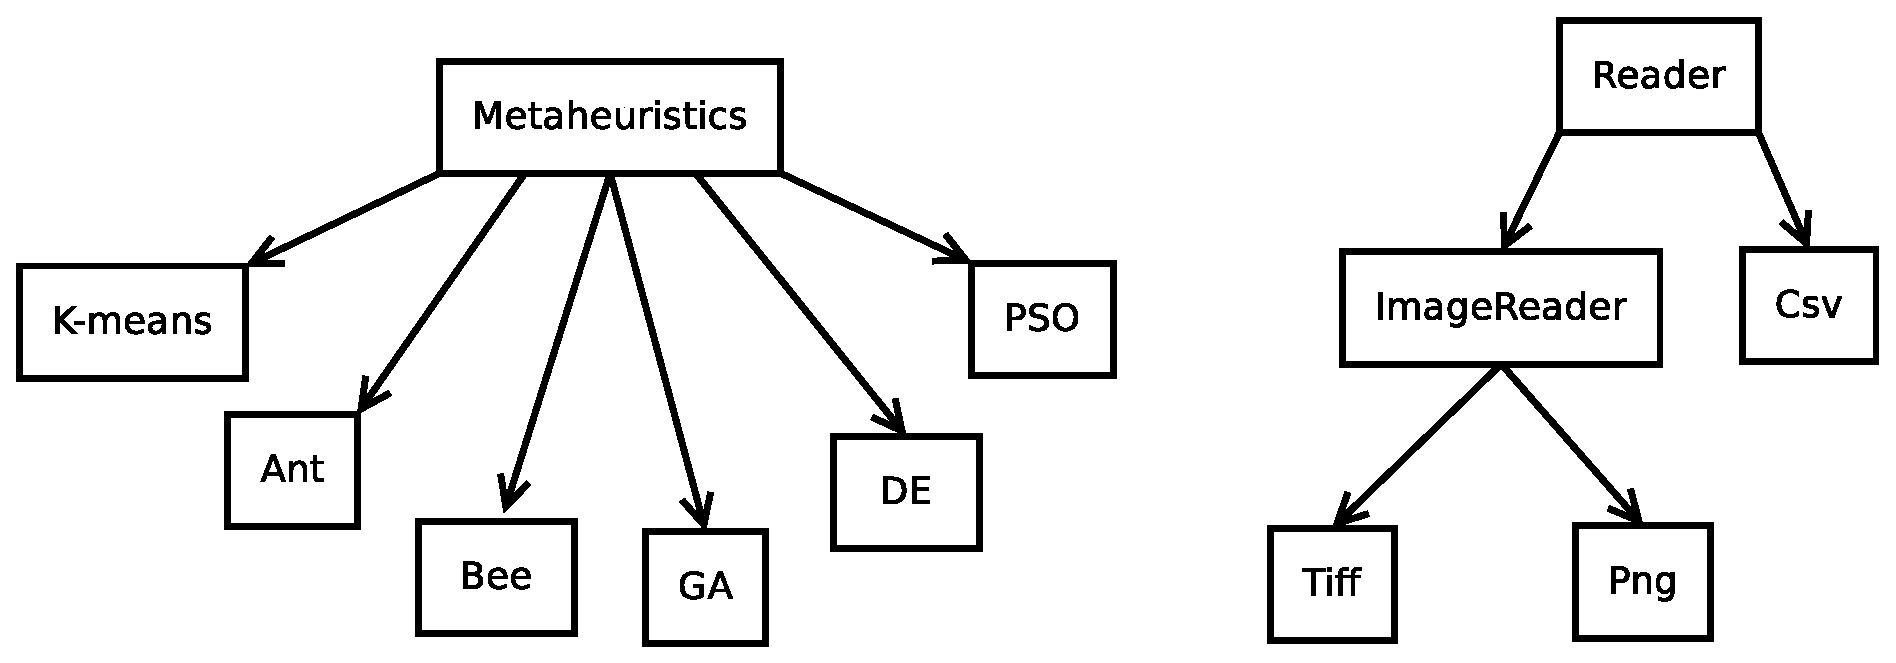
\includegraphics[scale=0.35]{figures/clases.eps}
\caption{Dise\~no de clases}
\label{fig:jclases}
\end{figure}

Donde Metaheuristics es una clase abstracta, que posee las m\'etodos que seran
usados por las diversas metaheur\'isticas hijas. En especial tienen dos 
importantes: initialize y run. El primero se va a encargar de inicializar el algoritmo
para que luego sea ejecutado. Por ejemplo en el gen\'etico inicializa aleatoriamente
las soluciones. Y el run es en s\'i el que va a ejecutar el algoritmo haciendo 
uso de los par\'ametros y variables ya inicilizadas.

Por el otro lado Reader tambi\'en
es una clase abstracta y es la que se encarga de definir lo m\'etodos que van a 
tener sus descendientes a la hora de leer un archivo, que se implement\'o para 
tres tipos: csv, png y tiff.

\section{M'aquina de prueba} \label{sect:testbed}

Todas las pruebas fueron realizadas con el computador cuyas caracter'isticas
aparecen en el cuadro \ref{tb:testbed}. La herramienta {\tt mhs} fue
compilada sobre esa m'aquina, exclusivamente con optimizaci'on gcc de nivel 3,
que es el nivel m\'as alto que posee gcc y aplica todas las mejoras
que este posee.

\begin{table}[htb]
\footnotesize
\begin{center}
\begin{tabular}{|>{\columncolor{lightgray}}c|c|}
\hline
CPU & Intel Core I5 650 \\
\hline
RAM & 6 GB \\
\hline
Distribuci'on & Ubuntu 11.04 x86\_64 bits \\
\hline
Kernel Linux & 2.6.38-8-generic \\
\hline
Versi'on gcc & 4.5.2 \\
\hline
\end{tabular}
\caption{Computador usado para las pruebas}
\label{tb:testbed}
\end{center}
\end{table}

\section{M\'etrica usada}

\section{K-means}

\'Este fue implementado tal cual como se explic\'o en \ref{sect:kmeans}. La
inicializaci\'on es totalmente aleatoria. Y la condici\'on de paradas
va a ser hasta que no se mejores un n\'umero de veces dado.

\section{Bee}

\section{Gen\'etico}

\section{DE}

\section{PSO}

\section{Hormiga}

Los resultados que se quieren evaluar est'an divididos en tres partes: 
Primero, es necesario verificar la calidad de estimaci'on del par'ametro
de Hurst usando los m'etodos implementados, segundo, es importante medir 
el tiempo necesario para cada estimaci'on y, por 'ultimo, es importante
comprobar si se pueden detectar ataques de denegaci'on de servicio mediante la
variaci'on del par'ametro y el uso del mecanismo de ventanas deslizantes.

La descripci'on del computador utilizado para ejecutar las pruebas se 
presenta en la secci'on \ref{sect:testbed}. Los archivos utilizados y los
resultados de la verificaci'on de la estimaci'on del par'ametro de Hurst y del
tiempo necesario para la estimaci'on se presentan en la secci'on
\ref{sect:validacion}. Estos resultandos muestran qu'e tan
preciso es la implementaci'on de los m'etodos y cu'anto tiempo en promedio
necesita la herramienta para estimar el valor del par'ametro de Hurst en una
ventana. 

\section{Validaci'on de los estimados} \label{sect:validacion}

Se ten'ia que probar que las implementaciones de los 3 m'etodos produc'ian
estimaciones razonables del par'ametro de Hurst para saber de antemano que tan
confiable podrian ser la estimaciones cuando se usasen junto con el mecanismo
de ventanas delizantes. Para la validaci'on de los m'etodos implementados se
probaron los mismos con datos producidos por el algoritmo de Paxson
\cite{Paxson95fastapproximation}.

El algoritmo de Paxson permite crear una serie de tiempo pseudo-aleatoria en
el dominio del tiempo de forma r'apida, y permite especificar el par'ametro de
Hurst a ser simulado y el n'umero de datos que debe tener la serie de tiempo
resultante, manteniendo la media en $0$ y la varianza en $1$, con valores
uniformemente distribuidos en el intervalo $[0,2\pi]$. Mediante el algoritmo
se puede simular un proceso estacionario autosimilar con dependencia de largo
alcance \cite{Paxson95fastapproximation}.

La implementaci'on del algoritmo de Paxson utilizada es la que viene en el 
paquete {\tt fArma} de {\tt R}. La validaci'on cont'o con 6 tama~nos diferentes
para la serie de tiempo $X_k$ generada por el algoritmo de Paxson. Estos 
tama~nos fueron $\{1024, 2048, 4096, 8192, 16384, 32768\}$. Por cada tama~no se
generaron 10 series de tiempo $X_k$ para cada uno de los 9 valores del
par'ametro de Hurst que se quer'ia simular. Estos valores fueron
$\{0.55, 0.60, 0.65, 0.70, 0.75, 0.80, 0.85, 0.90, 0.95 \}$. 
\begin{figure}[htb]
\centering
\includegraphics[scale=0.45,type=png,ext=.png,read=.png]{figures/abserror-rs}
\caption{Promedio y varianza del error absoluto de la estimaci'on del par'ametro
de Hurst para el m'etodo estad'istico R/S}
\label{fig:abserrrs}
\end{figure}

\begin{figure}[htb]
\centering
\includegraphics[scale=0.45,type=png,ext=.png,read=.png]{figures/abserror-var}
\caption{Promedio y varianza del error absoluto de la estimaci'on del par'ametro
de Hurst para el m'etodo de gr'aficas de varianza-tiempo}
\label{fig:abserrvar}
\end{figure}

\begin{figure}[htb]
\centering
\includegraphics[scale=0.45,type=png,ext=.png,read=.png]{figures/abserror-mavar}
\caption{Promedio y varianza del error absoluto de la estimaci'on del par'ametro
de Hurst para el m'etodo de varianza modificada de Allan}
\label{fig:abserrmavar}
\end{figure}

\clearpage

\begin{figure}[htb]
\centering
\includegraphics[scale=0.38,type=png,ext=.png,read=.png]{figures/time-n-plot}
\caption{Tiempo promedio utilizado para estimar una ventana de 1024 a 32768
datos para los m'etodos implementados}
\label{fig:tiempoventana}
\end{figure}

Observando las figuras \ref{fig:abserrrs}, \ref{fig:abserrvar} y
\ref{fig:abserrmavar}, lo que se puede evidenciar es que, en general, el
promedio del error absoluto de las estimaciones del par'ametro de Hurst de los
m'etodos mejoran y la varianza disminuye cuando se toman en cuenta un mayor
n'umero de datos para la ventana de estimaci'on. Sin embargo, para los
dos m'etodos que dependen de c'alculos con la varianza el promedio del error 
absoluto de la estimaci'on, incluso con el mayor n'umero de datos es mayor a
$0.1$. El m'etodo del estad'istico R/S es el m'etodo que se comporta mejora 
ya que tiene, en general, un error absoluto muy cerca a $0$ con una varianza
m'inima. 

De acuerdo a \cite{intelligentfuzzy} si queremos analizar los datos en tiempo
real para una red se tendr'ia que hacer una estimaci'on como m'inimo cada
segundo, por lo que una estimaci'on no puede tardar m'as de un segundo en
realizarse. Esto es seriamente limitante ya que cada m'etodo tiene un tiempo de
ejecuci'on muy diferente. Observando la figura \ref{fig:tiempoventana}, con
esta restricci'on la 'unica posibilidad que se tiene es limitar al m'etodo del
estad'istico R/S a $4096$ datos, al m'etodo de gr'aficas varianza-tiempo a
$16834$ datos y al m'etodo de varianza modificada de Allan a $4096$ datos. Dado
que para comparar los m'etodos es importante usar la misma cantidad de datos,
decidimos trabajar con $4096$ datos. El limitar el n'umero de datos va a
afectar la estimaci'on del par'ametro de Hurst directamente como se muestra en
las figuras \ref{fig:abserrrs}, \ref{fig:abserrvar} y \ref{fig:abserrmavar}. 

A pesar de estos problemas, seguimos adelante con el proyecto porque no
queremos una sola estimaci'on puntual y precisa de la traza, sino detectar su
variaci'on, por lo que optamos por un buen balance entre el tiempo de
ejecuci'on y el n'umero de datos a utilizar \cite{intelligentfuzzy}.



% Resultados
\chapter{Pruebas experimentales} \label{sect:impresultados}

\section{Máquina de pruebas} \label{sect:testbed}

    Todas las pruebas fueron realizadas con un computador cuyas características
aparecen en la tabla \ref{tb:testbed}. El programa implementado, de nombre
{\bf mhs}, fue compilado con \emph{gcc} con optimización de nivel 3 en la
máquina mencionada anteriormente. Se eligió ese nivel de optimización ya que
aplica todas las mejoras del compilador \emph{gcc}.

\begin{table}[htb]
\footnotesize
\begin{center}
\begin{tabular}{|>{\columncolor{lightgray}}c|c|}
\hline
CPU & Intel Core I5 650 \\
\hline
RAM & 6 GB \\
\hline
Distribución & Ubuntu 11.04 x86\_64 bits \\
\hline
Kernel Linux & 2.6.38-8-generic \\
\hline
Versión gcc & 4.5.2 \\
\hline
\end{tabular}
\caption{Computador usado para las pruebas}
\label{tb:testbed}
\end{center}
\end{table}

\section{Formato de pruebas}  
\label{sect:ajustep}

    Se buscó el conjunto de mejores valores para los parámetros de cada algoritmo
implementado. Algunos de estos parámetros se mantuvieron fijos, decisión tomada
a partir de pruebas experimentales o recomendaciones de artículos y libros. Para
ello se realizaron dos conjuntos de pruebas y análisis:

\begin{enumerate}
    \item \emph{Pruebas con análisis de varianza}(ver apéndice \ref{apendiceb}):
            Para las pruebas, se recabó información de cada metaheurística de la
        siguiente forma:
        \begin{enumerate}
            \item Se generaron valores para el conjunto de parámetros de cada
        metaheurística, a partir de la permutación de rangos discretos válidos para cada
        uno de los mismos (véanse las secciones \ref{sect:iga-rv}, \ref{sect:iwpso-rv},
        \ref{sect:inpso-rv}, \ref{sect:inde-rv}, \ref{sect:isde-rv},
        \ref{sect:ibee-rv} y \ref{sect:iant-rv}).
            \item Se ejecutó cada metaheurística con cada uno de los conjunto de
        valores generados anteriormente y se extrajo el valor de la función de
        \emph{fitness} $f$ de cada solución final.
        \end{enumerate}
	\item \emph{Pruebas exhaustivas} (ver apéndice \ref{apendicea}):
            Para las pruebas, se recabó información de cada metaheurística de la
        siguiente forma:
        \begin{enumerate}
            \item Se generaron valores para el conjunto de parámetros de cada
        metaheurística a partir de la permutación de rangos discretos válidos para cada
        uno de los mismos (véanse las secciones  \ref{sect:agenetico}, \ref{sect:anpso},
        \ref{sect:awpso}, \ref{sect:ande}, \ref{sect:asde}, \ref{sect:abee},
        \ref{sect:aant}).
            \item Se ejecutó cinco veces cada metaheurística con cada uno de los     
        conjunto de valores generados anteriormente.
            \item De los resultados obtenidos, se promediaron las cinco corridas de cada
        metaheurística y se tomaron los veinte mejores conjunto de valores.
            \item Cada metaheurística fue ejecutada nuevamente con cada uno de los veinte
        mejores conjuntos de valores para ella. Fueron ejecutadas treinta veces para
        cada conjunto de valores.
        \end{enumerate}
\end{enumerate}

\subsection{Metaheurísticas híbridas}\label{exp:hibrido}

    Adicionalmente a la implementación de las metaheurísticas, también se implementaron
híbridos de éstas con el algoritmo determinista \emph{K-means}. En otras palabras,
las soluciones finales de cada metaheurística eran mejoradas por el algoritmo
\emph{K-means}.

    Se realizaron las \emph{pruebas exhaustivas} descritas anteriormente (ver
sección \ref{sect:ajustep}) tanto con las metaheurísticas híbridas como para las
no híbridas para luego hacer un análisis comparativo de las mismas (ver apéndice
\ref{apendicec}).

    Se utilizaron las metaheurísticas híbridas para hacer los análisis comparativos
del capítulo \ref{chap:analisis} ya que tuvieron mejor calidad de soluciones
finales que sus contrapartes no híbridas (ver apendice \ref{apendicec}).

\subsection{Archivos de prueba}\label{datatest}

    Las pruebas mencionadas anteriormente (ver sección \ref{sect:ajustep}) se
realizaron para los conjuntos de datos mostrados a continuación:
\begin{itemize}

\item {\bf Lenna:}\label{test:lenna} Es una imagen muy usada por los investigadores en el área 
de imágenes (ver figura
\subref{fig:lenna}). 
\textbf{El número óptimo de clusters está en el rango $[5,10]$\cite{OuBa2007}.}
Se usó una versión de resolución 128x128.

\item {\bf Iris:}\label{test:iris} Es un conjunto bastante conocido de datos que
consiste en tres diferentes especies de la planta iris: \emph{Iris setosa},
\emph{Iris virginica} e \emph{Iris versicolour}. Para cada una de las especies,
hay 50 muestras con cuatro atributos de tipo real: longitud del sépalo, ancho
del sépalo, longitud de pétalos y ancho de pétalos. \textbf{La partición óptima
es de 3 clusters con 50 objetos cada uno, de los cuales cada cluster representa a
una de las especies \cite{SwAjAm2008}.}

\item {\bf Imagen sintética:} Es una imagen creada con la finalidad de ver
gráficamente el buen funcionamiento
de las metaheurísticas implementadas (ver figura \subref{fig:Trivial}). \textbf{Al
ser una imagen simple, un buen
algoritmo debería encontrar la partición óptima (7 clusters: 6 figuras bien
diferenciadas y el fondo) sin ninguna dificultad.}

\end{itemize}

\begin{figure}[h!]
  \centering
  \subfloat[\emph{Lenna}]{\label{fig:lenna}\includegraphics{figures/lenamini.png}} \qquad
  \subfloat[\emph{Imagen sintética}]{\label{fig:Trivial}\includegraphics[scale=0.3]{figures/trivial.png}}
  \caption{Imágenes de prueba usadas}
  \label{fig:imgs}
\end{figure}

\subsection{Formato de las tablas de resultados}

    A continuación, se presentan los significados de las abreviaturas de las
cabeceras de las tablas de resultados:
\begin{itemize}
    \item \textbf{FO}: Valor de la función de \emph{fitness} $1/DB$ para la
solución final.
    \item \textbf{DB}: Valor del índice \emph{DB} para la solución final.
    \item \textbf{$J_e$}: Valor de la cuantificación del error para la solución
final.
	\item \textbf{E}:Cantidad de evaluaciones de la función de \emph{fitness}.
\end{itemize}

\section{Resultados del K-means}

    En esta sección, se muestran los resultados del algoritmo determinista
\emph{K-means}.

\subsection{Resultados obtenidos para \textbf{Lenna}}

    A continuación, se presenta una tabla resumen de 30 ejecuciones del
algoritmo \emph{K-means} con la imagen \textbf{Lenna}:

\begin{table}[h!]
\footnotesize
\begin{center}
\begin{tabular}{|c|c|c|c|c|}
\hline
&{\bf FO}&{\bf DB}&{\bf $J_e$}\\
\hline
\hline
Promedio & 1.2037 & 0.8333 & 17.1739\\
\hline
Mejor & 1.2797 & 0.7814 & 16.9164\\
\hline
Peor & 1.0456 & 0.9564 & 17.091\\
\hline
\end{tabular}
\caption{Resultados de \emph{K-means} para {\bf Lenna}}
\label{tb:pmpkmeansimg}
\end{center}
\end{table}


\subsection{Resultados obtenidos para \textbf{Iris}}

    A continuación, se presenta una tabla resumen de 30 ejecuciones del
algoritmo \emph{K-means} con el archivo de datos numéricos \textbf{Iris}:

\begin{table}[h!]
\footnotesize
\begin{center}
\begin{tabular}{|c|c|c|c|c|}
\hline
&{\bf FO}&{\bf DB}&{\bf $J_e$}\\
\hline
\hline
Promedio & 1.4915 & 0.6756 & 0.64\\
\hline
Mejor & 1.6695 & 0.599 & 0.6339\\
\hline
Peor & 0.9983 & 1.0017 & 0.7094\\
\hline
\end{tabular}
\caption{Resultados de \emph{K-means} para {\bf Lenna}}
\label{tb:pmpkmeanscsv}
\end{center}
\end{table}


\section{Resultados del \emph{GA}}

    En esta sección, se muestran los resultados del algoritmo genético híbrido con
\emph{K-means} (\emph{GAH}) para la imagen \textbf{Lenna} y el archivo de datos
numéricos \textbf{Iris} (ver sección \ref{exp:hibrido}).

\subsection{Parámetros variables}\label{sect:iga-pv}

    A continuación, se describen los parámetros variables del algoritmo:
\begin{itemize}
    \item $I$: representa a la cantidad total de individuos de la población,
donde $I \geq 2$.
    \item $tt$: representa el tamaño del torneo, donde $tt \geq 2$ y $tt \leq I$.
    \item $pc$: representa la probabilidad de cruce de los individuos y
está acotado en el rango $[0, 1]$.
    \item $pm$: representa la probabilidad de mutación de los individuos y
está acotado en el rango $[0, 1]$.
\end{itemize}

\subsubsection{Resultados obtenidos para \textbf{Lenna}}

    A continuación, se presenta una tabla resumen de 30 ejecuciones del mejor
conjunto de valores para los parámetros del algoritmo \emph{GAH}:

\begin{table}[h!]
\footnotesize
\begin{center}
\begin{tabular}{|c|c|c|c|c|c|c|c|c|c|}
\hline
& {\bf FO} & {\bf DB}& $J_e$ & $I$ & $tt$ & $pc$ & $pm$ \\
\hline
\hline
Promedio   & 1.2753 & 0.7853  & 17.5582 &  &  &  & \\
\cline{1-4}
Mejor & 1.4104 & 0.709  & 19.4009 & 10 & 4 & 0.8 & 1.0\\
\cline{1-4}
Peor & 1.179 & 0.8481  & 17.6034 &  &  &  & \\\hline
\end{tabular}
\caption{Resultados de las mejores corridas de \emph{GAH} para {\bf Lenna}}
\label{tb:pmpgahibimg}
\end{center}
\end{table}


\subsubsection{Resultados obtenidos para \textbf{Iris}}

    A continuación, se presenta una tabla resumen de 30 ejecuciones del mejor
conjunto de valores para los parámetros del algoritmo \emph{GAH}:

\begin{table}[h!]
\footnotesize
\begin{center}
\begin{tabular}{|c|c|c|c|c|c|c|c|c|c|}
\hline
& {\bf FO} & {\bf DB}& $J_e$ & $I$ & $tt$ & $pc$ & $pm$ \\
\hline
\hline
Promedio   & 2.6521 & 0.3771  & 0.5029 &  &  &  & \\
\cline{1-4}
Mejor & 2.6521 & 0.3771  & 0.5029 & 25 & 12 & 0.2 & 1.0\\
\cline{1-4}
Peor & 2.6521 & 0.3771  & 0.5029 &  &  &  & \\\hline
\end{tabular}
\caption{Resultados de las mejores corridas de \emph{GAH} para {\bf Iris}}
\label{tb:pmpgahibcsv}
\end{center}
\end{table}


\subsubsection{Influencia de los parámetros}

Teniendo en cuenta que el \emph{rango probado} es el conjunto de valores utilizado
para las pruebas y el \emph{rango efectivo} es el conjunto valores de los parámetros
para los 20 mejores resultados del algoritmo \emph{GAH} (tablas \ref{tb:tablegahibimg}
y \ref{tb:tablegahibcsv}), se encontró lo siguiente:

\begin{itemize}
    \item Para la imagen \textbf{Lenna}:
        \begin{itemize}
            \item Parámetro $I$:
                Como el \emph{rango probado} ($[5, 40]$) es
                igual al \emph{rango efectivo} ($[5, 40]$) no importa que valor tome el
                parámetro $I$, el \emph{GAH} puede dar una buena solución
                final. Por lo tanto, este parámetro no influye
                considerablemente en la bondad de la solución final.
            \item Parámetro $tt$:
                Como el \emph{rango probado}($[4, 40]$) es
                mayor al \emph{rango efectivo} ($[4, 24]$), es relevante el valor que se
                le asigne al parámetro $tt$. \textbf{Por lo tanto, este
                parámetro influye en la bondad de la solución final.}
            \item Parámetro $pc$:
                Como el \emph{rango probado}($[0.0; 1.0]$) es
                practicamente igual al \emph{rango efectivo} (sólo faltan el $0.4$ y $0.9$), 
                no importa que valor tome el
                parámetro $pc$, el \emph{GAH} puede dar una buena solución
                final. Por lo tanto, este parámetro no influye
                considerablemente en la bondad de la solución final.
            \item Parámetro $pm$:
                Como el \emph{rango probado}($[0.1; 1.0]$ ) es
                mayor al \emph{rango efectivo} ($[0.5; 1.0]$ ), es relevante el valor que se
                le asigne al parámetro $pm$. \textbf{Por lo tanto, este
                parámetro influye en la bondad de la solución final.}
        \end{itemize}
	\item Para el archivo numérico \textbf{Iris}:
        \begin{itemize}
            \item Parámetro $I$:
                Como el \emph{rango probado}($[5, 40]$) es
                mayor al \emph{rango efectivo} ($[25, 40]$), es relevante el valor que se
                le asigne al parámetro $I$. \textbf{Por lo tanto, este
                parámetro influye en la bondad de la solución final.}
			\item Para los parámetros $tt$, $pc$ y $pm$ se observa un comportamiento
				similar al encontrado para la imagen \textbf{Lenna}.
        \end{itemize}
\end{itemize}

\section{Resultados del \emph{WPSO}}

    En esta sección, se muestran los resultados de la metaheurística \emph{WPSO}
híbrida con \emph{K-means} (\emph{WPSOH\-}) para la imagen \textbf{Lenna}
y el archivo de datos numéricos \textbf{Iris} (ver sección \ref{exp:hibrido}).

\subsection{Parámetros variables}\label{sect:iwpso-pv}

    A continuación, se describen los parámetros variables del algoritmo:
\begin{itemize}
    \item $I$: representa a la cantidad total de partículas del enjambre,
donde $I \geq 2$.
    \item $w_1$, $w_2$ y $w_3$: son los pesos de la función de \emph{fitness}
(\ref{pso: wpso}), deben ser positivos y su suma debe ser igual a 1.
    \item $W$, $c_1$ y $c_2$: representan al peso inercial, factor de aprendizaje
colectivo y factor de aprendizaje social, respectivamente, descritos en la
sección \ref{sect:metapso-vel}. $W$ debe estar acotado en el rango $[0, 2]$ y
$c_1$ y $c_2$ deben satisfacer la inecuación (\ref{pso: convergece}).
    \item $vmx$: es un escalar, acotado en el rango $[0, 1]$, que multiplica al
vector $Z_{max}$ con el fin de regular la velocidad máxima de la partícula,
donde $vmx \cdot Z_{max}$ es el valor máximo de la velocidad $v(t)$ (véase la
ecuación (\ref{pso: vi})).
\end{itemize}

\subsubsection{Resultados obtenidos para \textbf{Lenna}}
    A continuación, se presenta una tabla resumen de 30 ejecuciones del mejor
conjunto de valores para los parámetros del algoritmo \emph{WPSOH}:

\begin{table}[h!]
\footnotesize
\begin{center}
\begin{tabular}{|c|c|c|c|c|c|c|c|c|c|c|c|c|c|}
\hline
& {\bf FO} & {\bf DB}& $J_e$ & $I$ & $w_1$ & $w_2$ & $w_3$ & $W$ & $c_1$ & $c_2$ & $vmx$ \\
\hline
\hline
Promedio   & 1.2005 & 0.8348  & 17.7634 &  &  &  &  &  &  &  & \\
\cline{1-4}
Mejor & 1.3039 & 0.7669  & 16.9839 & 35 & 0.0 & 1.0 & 0.0 & 0.5 & 2.0 & 0.5 & 0.5\\
\cline{1-4}
Peor & 1.1074 & 0.903  & 17.6885 &  &  &  &  &  &  &  & \\\hline
\end{tabular}
\caption{Resultados de las mejores corridas de \emph{WPSOH} para {\bf Lenna}}
\label{tb:pmpwpsohibimg}
\end{center}
\end{table}


\subsubsection{Resultados obtenidos para \textbf{Iris}}

    A continuación, se presenta una tabla resumen de 30 ejecuciones del mejor
conjunto de valores para los parámetros del algoritmo \emph{WPSOH}:

\begin{table}[h!]
\footnotesize
\begin{center}
\begin{tabular}{|c|c|c|c|c|c|c|c|c|c|c|c|c|c|}
\hline
& {\bf FO} & {\bf DB}& $J_e$ & $I$ & $w_1$ & $w_2$ & $w_3$ & $W$ & $c_1$ & $c_2$ & $vmx$ \\
\hline
\hline
Promedio   & 1.5694 & 0.6385  & 0.661 &  &  &  &  &  &  &  & \\
\cline{1-4}
Mejor & 1.6992 & 0.5885  & 0.6709 & 10 & 0.8 & 0.2 & 0.0 & 0.8 & 1.1 & 1.1 & 0.5\\
\cline{1-4}
Peor & 1.5165 & 0.6594  & 0.6466 &  &  &  &  &  &  &  & \\\hline
\end{tabular}
\caption{Resultados de las mejores corridas de \emph{WPSOH} para {\bf Iris}}
\label{tb:pmpwpsohibcsv}
\end{center}
\end{table}


\subsubsection{Influencia de los parámetros}

Teniendo en cuenta que el \emph{rango probado} es el conjunto de valores utilizado
para las pruebas y el \emph{rango efectivo} es el conjunto valores de los parámetros
para los 20 mejores resultados del algoritmo \emph{WPSOH} (tablas \ref{tb:tablewpsohibimg}
y \ref{tb:tablewpsohibcsv}), se encontró lo siguiente:

\begin{itemize}
	\item Para la imagen \textbf{Lenna}:
	\begin{itemize}
		\item No se puede encontrar una relación entre los valores de los
			parámetros y el valor de la función de \emph{fitness}. Se
			puede observar que para cada parámetro el \emph{rango efectivo}
			es similar \emph{rango probado}. Esto indica que el valor que tome cada
			uno de los parámetros del algoritmo parece no tener una gran influencia en la
			solución final.
	\end{itemize}
	\item Para el archivo numérico \textbf{Iris}:
	\begin{itemize}
		\item Se puede observar que los parámetros $I$, $w_1$, $w_2$, $w_3$ y
			$W$ pueden ser fijados en $10$, $0.8$, $0.2$, $0.0$ y $0.8$,
			respectivamente. Los demás parámetros se comportan de manera similar 
			a como lo hacen para la imagen {\bf Lenna}.
	\end{itemize}
\end{itemize}

\section{Resultados del \emph{NPSO}}

    En esta sección, se muestran los resultados de la metaheurística \emph{NPSO}
híbrida con \emph{K-means} (\emph{NPSOH}) para la imagen \textbf{Lenna} y el archivo
de datos numéricos \textbf{Iris} (ver sección \ref{exp:hibrido}).

\subsection{Parámetros variables}\label{sect:inpso-pv}

    Los parámetros variables son los mismos descritos en la sección \ref{sect:iwpso-pv},
exceptuando los pesos $w_1$, $w_2$ y $w_3$.

\subsubsection{Resultados obtenidos para \textbf{Lenna}}

    A continuación, se presenta una tabla resumen de 30 ejecuciones del mejor
conjunto de valores para los parámetros del algoritmo \emph{NPSOH}:

\begin{table}[h!]
\footnotesize
\begin{center}
\begin{tabular}{|c|c|c|c|c|c|c|c|c|c|c|}
\hline
& {\bf FO} & {\bf DB}& $J_e$ & $I$ & W & $c_1$ & $c_2$ & $vmx$ \\
\hline
\hline
Promedio   & 1.2071 & 0.8297  & 17.5799 & &  &  &  & \\
\cline{1-4}
Mejor & 1.2968 & 0.7711  & 17.3749 & 35 & 0.8 & 1.7 & 1.7 & 0.5\\
\cline{1-4}
Peor & 1.1113 & 0.8999  & 19.3463 &  &  &  &  & \\\hline
\end{tabular}
\caption{Resultados de las mejores corridas de \emph{NPSOH} para {\bf Lenna}}
\label{tb:pmppsohibimg}
\end{center}
\end{table}


\subsubsection{Resultados obtenidos para \textbf{Iris}}

    A continuación, se presenta una tabla resumen de 30 ejecuciones del mejor
conjunto de valores para los parámetros del algoritmo \emph{NPSOH}:

\begin{table}[h!]
\footnotesize
\begin{center}
\begin{tabular}{|c|c|c|c|c|c|c|c|c|c|c|}
\hline
& {\bf FO} & {\bf DB}& $J_e$ & $I$ & W & $c_1$ & $c_2$ & $vmx$ \\
\hline
\hline
Promedio   & 1.5654 & 0.6395  & 0.6606 &  &  &  &  & \\
\cline{1-4}
Mejor & 1.6626 & 0.6015  & 0.6807 & 25 & 1.1 & 1.7 & 0.5 & 0.5\\
\cline{1-4}
Peor & 1.5006 & 0.6664  & 0.649 &  &  &  &  & \\\hline
\end{tabular}
\caption{Resultados de las mejores corridas de \emph{NPSOH} para {\bf Iris}}
\label{tb:pmppsohibcsv}
\end{center}
\end{table}


\subsubsection{Influencia de los parámetros}

Teniendo en cuenta que el \emph{rango probado} es el conjunto de valores utilizado
para las pruebas y el \emph{rango efectivo} es el conjunto valores de los parámetros
para los 20 mejores resultados del algoritmo \emph{NPSOH} (tablas \ref{tb:tablepsohibimg}
y \ref{tb:tablepsohibcsv}), se encontró lo siguiente:

\begin{itemize}
	\item Para la imagen \textbf{Lenna}:
	\begin{itemize}
		\item No se puede encontrar una relación entre los valores de los
			parámetros y el valor de la función de \emph{fitness}. Se
			puede observar que para cada parámetro el \emph{rango efectivo}
			es similar \emph{rango probado}. Esto indica que el valor que tome cada
			uno de los parámetros del algoritmo parece no tener una gran influencia en la
			solución final.
	\end{itemize}
	\item Para el archivo numérico \textbf{Iris}:
	\begin{itemize}
		\item Se puede observar que los parámetros $I$ y $W$ pueden ser fijados
			en $25$ y $1.1$, respectivamente. Los demás parámetros se comportan de manera similar 
			a como lo hacen para la imagen {\bf Lenna}.
	\end{itemize}
\end{itemize}

\section{Resultados del \emph{SDE}}

    En esta sección, se muestran los resultados de la metaheurística  \emph{SDE}
híbrida con \emph{K-means} (\emph{SDEH}) para la imagen \textbf{Lenna} y el
archivo de datos numéricos \textbf{Iris} (ver sección \ref{exp:hibrido}).

\subsection{Parámetros variables}\label{sect:isde-pv}

    A continuación, se describen los parámetros variables del algoritmo:
\begin{itemize}
    \item $I$: representa a la cantidad total de individuos, donde $I \geq 4$.
    \item $w_1$, $w_2$ y $w_3$: son los pesos de la función de \emph{fitness}
(\ref{pso: wpso}), deben ser positivos y su suma debe ser igual a 1.
    \item $\gamma$: factor de escalados de la diferencia. Está acotado en el rango $[0, 1]$.
    \item $Cr$: representa la probabilidad de cruce  de los individuos y
está acotado en el rango $[0, 1]$.
\end{itemize}

\subsubsection{Resultados obtenidos para \textbf{Lenna} (\emph{SDEH})}

    A continuación, se presenta una tabla resumen de 30 ejecuciones del mejor
conjunto de valores para los parámetros del algoritmo \emph{SDEH}:

\begin{table}[h!]
\footnotesize
\begin{center}
\begin{tabular}{|c|c|c|c|c|c|c|c|c|c|c|c|}
\hline
& {\bf FO} & {\bf DB}& $J_e$ & $I$ & $w_1$ & $w_2$ & $w_3$ & $\gamma$ & $Cr$ \\
\hline
\hline
Promedio   & 1.1813 & 0.8491  & 19.5178 &  &  &  &  &  & \\
\cline{1-4}
Mejor & 1.3195 & 0.7578  & 16.9559 & 10 & 0.4 & 0.5 & 0.1 & 0.5 & 0.7\\
\cline{1-4}
Peor & 0.9948 & 1.0052  & 39.0413 &  &  &  &  &  & \\\hline
\end{tabular}
\caption{Resultados de las mejores corridas de \emph{SDEH} para {\bf Lenna}}
\label{tb:pmpsdehibimg}
\end{center}
\end{table}


\subsubsection{Resultados obtenidos para \textbf{Iris} (\emph{SDEH})}

    A continuación, se presenta una tabla resumen de 30 ejecuciones del mejor
conjunto de valores para los parámetros del algoritmo \emph{SDEH}:

\begin{table}[h!]
\footnotesize
\begin{center}
\begin{tabular}{|c|c|c|c|c|c|c|c|c|c|c|c|}
\hline
& {\bf FO} & {\bf DB}& $J_e$ & $I$ & $w_1$ & $w_2$ & $w_3$ & $\gamma$ & $Cr$ \\
\hline
\hline
Promedio   & 1.5312 & 0.6533  & 0.6448 &  &  &  &  &  & \\
\cline{1-4}
Mejor & 1.5778 & 0.6338  & 0.625 & 15 & 0.5 & 0.1 & 0.4 & 0.8 & 0.9\\
\cline{1-4}
Peor & 1.5006 & 0.6664  & 0.649 &  &  &  &  &  & \\\hline
\end{tabular}
\caption{Resultados de las mejores corridas de \emph{SDEH} para {\bf Iris}}
\label{tb:pmpsdehibcsv}
\end{center}
\end{table}


\subsubsection{Influencia de los parámetros}

Teniendo en cuenta que el \emph{rango probado} es el conjunto de valores utilizado
para las pruebas y el \emph{rango efectivo} es el conjunto valores de los parámetros
para los 20 mejores resultados del algoritmo \emph{SDEH} (tablas \ref{tb:tablesdehibimg}
y \ref{tb:tablesdehibcsv}), se encontró lo siguiente:

\begin{itemize}
    \item Para la imagen {\bf Lenna}:
		\begin{itemize}
		    \item Para los parámetros $I$, $w_1$ y $w_3$ el \emph{rango efectivo}
				  es similar \emph{rango probado}. Esto
				  puede indicar que no influyen considerablemente en la calidad
				  de las soluciones finales.
		    \item Para los parámetros $\gamma$ y $Cr$  el \emph{rango efectivo} 
		          posee una gran cantidad de valores del \emph{rango probado}.
		          Esto puede indicar que no influyen considerablemente en la
		          calidad de las soluciones finales.
		    \item Parámetro $w_2$:
		          Como el \emph{rango probado}($[0.1; 1.0]$) es
		          mayor al \emph{rango efectivo} ($[0.0;0.8]$), es relevante el valor que se
		          le asigne al parámetro $w_2$. \textbf{Por lo tanto, este
		          parámetro influye en la bondad de la solución final.}
	    \end{itemize}
    
    \item Para el archivo numérico {\bf Iris}:
		\begin{itemize}
			\item Se puede observar que los parámetros $I$, $w_1$, $w_2$ y $w_3$
			  	  pueden ser fijados en  $15$, $0.5$, $0.1$ y $0.4$,
				  respectivamente. 
		    \item Parámetro $\gamma$:
		          Como el \emph{rango probado}($[0.5; 1.0]$) es
		          mayor al \emph{rango efectivo} ($[0.5;0.8]$), es relevante el valor que se
		          le asigne al parámetro $\gamma$. Además, mientras más alto
		          sea su valor, mejor es el valor de la función de \emph{fitness}.
		           \textbf{Por lo tanto, este
		          parámetro influye en la bondad de la solución final.}
		    \item Parámetro $Cr$:
		    	  Tiene un comportamiento similar al obtenido con \textbf{Lenna}.
		\end{itemize}
\end{itemize}

\section{Resultados del \emph{NDE}}

    En esta sección, se muestran los resultados de la metaheurística \emph{NDE}
híbrido con \emph{K-means} (\emph{NDEH}) para la imagen \textbf{Lenna} y el
archivo de datos numéricos \textbf{Iris} (ver sección \ref{exp:hibrido}).

\subsection{Parámetros variables}\label{sect:inde-pv}

    Los parámetros son los mismos que para el algoritmo \emph{SDEH} (ver la sección
\ref{sect:isde-pv}). Sin embargo, se calculan automáticamente los parámetros
$\gamma$ y $Cr$.

\subsubsection{Resultados obtenidos para \textbf{Lenna} (\emph{NDEH})}

    A continuación, se presenta una tabla resumen de 30 ejecuciones del mejor
conjunto de valores para los parámetros del algoritmo \emph{NDEH}:

\begin{table}[h!]
\footnotesize
\begin{center}
\begin{tabular}{|c|c|c|c|c|c|c|c|c|c|}
\hline
& {\bf FO} & {\bf DB}& $J_e$ & $I$ & $w_1$ & $w_2$ & $w_3$ \\
\hline
\hline
Promedio   & 1.2132 & 0.8256  & 19.9024 &  &  &  & \\
\cline{1-4}
Mejor & 1.3346 & 0.7493  & 16.589 & 40 & 0.0 & 0.0 & 1.0\\
\cline{1-4}
Peor & 1.1097 & 0.9011  & 17.6334 &  &  &  & \\\hline
\end{tabular}
\caption{Resultados de las mejores corridas de \emph{NDEH} para {\bf Lenna}}
\label{tb:pmpdehibimg}
\end{center}
\end{table}


\subsubsection{Resultados obtenidos para \textbf{Iris} (\emph{NDEH})}

    A continuación, se presenta una tabla resumen de 30 ejecuciones del mejor
conjunto de valores para los parámetros del algoritmo \emph{NDEH}:

\begin{table}[h!]
\footnotesize
\begin{center}
\begin{tabular}{|c|c|c|c|c|c|c|c|c|c|}
\hline
& {\bf FO} & {\bf DB}& $J_e$ & $I$ & $w_1$ & $w_2$ & $w_3$ \\
\hline
\hline
Promedio   & 1.5638 & 0.6403  & 0.6367 &  &  &  & \\
\cline{1-4}
Mejor & 1.7153 & 0.583  & 0.6586 & 15 & 0.2 & 0.7 & 0.1\\
\cline{1-4}
Peor & 1.5006 & 0.6664  & 0.649 &  &  &  & \\\hline
\end{tabular}
\caption{Resultados de las mejores corridas de \emph{NDEH} para {\bf Iris}}
\label{tb:pmpdehibcsv}
\end{center}
\end{table}


\subsubsection{Influencia de los parámetros}

Teniendo en cuenta que el \emph{rango probado} es el conjunto de valores utilizado
para las pruebas y el \emph{rango efectivo} es el conjunto valores de los parámetros
para los 20 mejores resultados del algoritmo \emph{NDEH} (tablas \ref{tb:tabledehibimg}
y \ref{tb:tabledehibcsv}), se encontró lo siguiente:

\begin{itemize}
    \item Para la imagen {\bf Lenna}:
		\begin{itemize}
		    \item Para los parámetros $I$, $w_1$ y $w_3$ el \emph{rango efectivo}
				  es similar \emph{rango probado}. Esto
		          puede indicar que no influyen considerablemente en la calidad
		          de las soluciones finales.
		    \item Parámetro $w_2$:
		          Como el \emph{rango probado}($[0.1; 1.0]$) es
		          mayor al \emph{rango efectivo} ($[0.0;0.6]$), es relevante el valor que se
		          le asigne al parámetro $w_2$. \textbf{Por lo tanto, este
		          parámetro influye en la bondad de la solución final.}
		\end{itemize}
    \item Para el archivo numérico {\bf Iris}:
		\begin{itemize}
		    \item A diferencia de los resultados para \emph{Lenna}, ningún
		    parámetro parece influir considerablemente en la calidad de las
		    soluciones finales.
		\end{itemize}
\end{itemize}

\section{Resultados del \emph{Bee}}

    En esta sección, se muestran los resultados del algoritmo de abeja híbrido con
\emph{K-means} (\emph{BeeH}) para la imagen \textbf{Lenna} y el archivo de datos
numéricos \textbf{Iris} (ver sección \ref{exp:hibrido}).

\subsection{Parámetros variables}\label{sect:ibee-pv}

    A continuación, se describen los parámetros variables del algoritmo:
\begin{itemize}
    \item $I$: Representa a la cantidad total de abejas del enjambre,
donde $I \geq 2$.
    \item $m$: Representa los sitios de flores totales, donde $m < I$.
    \item $e$: Representa los sitios de flores élite, donde $e < m$.
    \item $eb$ y $ob$: Representan la cantidad de abejas élite y la cantidad de
abejas exploradoras, respectivamente, donde $eb + ob \leq I$.
\end{itemize}

\subsubsection{Resultados obtenidos para \textbf{Lenna}}

    A continuación, se presenta una tabla resumen de 30 ejecuciones del mejor
conjunto de valores para los parámetros del algoritmo \emph{BeeH}:

\begin{table}[h!]
\footnotesize
\begin{center}
\begin{tabular}{|c|c|c|c|c|c|c|c|c|c|c|}
\hline
& {\bf FO} & {\bf DB}& $J_e$ & $I$ & $m$ & $e$ & $eb$ & $ob$ \\
\hline
\hline
Promedio   & 1.3052 & 0.7664  & 16.924 &  &  &  &  & \\
\cline{1-4}
Mejor & 1.3624 & 0.734  & 16.9922 & 35 & 15 & 2 & 14 & 6\\
\cline{1-4}
Peor & 1.2586 & 0.7945  & 16.7638 &    &  &  &  & \\\hline
\end{tabular}
\caption{Resultados de las mejores corridas de \emph{BeeH} para {\bf Lenna}}
\label{tb:pmpbeehibimg}
\end{center}
\end{table}


\pagebreak

\subsubsection{Resultados obtenidos para \textbf{Iris}}

    A continuación, se presenta una tabla resumen de 30 ejecuciones del mejor
conjunto de valores para los parámetros del algoritmo \emph{BeeH}:

\begin{table}[h!]
\footnotesize
\begin{center}
\begin{tabular}{|c|c|c|c|c|c|c|c|c|c|c|}
\hline
& {\bf FO} & {\bf DB}& $J_e$ & $I$ & $m$ & $e$ & $eb$ & $ob$ \\
\hline
\hline
Promedio   & 1.9167 & 0.5412  & 0.6281 &  &  &  &  & \\
\cline{1-4}
Mejor & 2.6521 & 0.3771  & 0.5029 & 30 & 15 & 12 & 6 & 9\\
\cline{1-4}
Peor & 1.6451 & 0.6079  & 0.6287 &  &  &  &  & \\\hline
\end{tabular}
\caption{Resultados de las mejores corridas de \emph{BeeH} para {\bf Iris}}
\label{tb:pmpbeehibcsv}
\end{center}
\end{table}


\subsubsection{Influencia de los parámetros}

Teniendo en cuenta que el \emph{rango probado} es el conjunto de valores utilizado
para las pruebas y el \emph{rango efectivo} es el conjunto valores de los parámetros
para los 20 mejores resultados del algoritmo \emph{BeeH} (tablas \ref{tb:tablebeehibimg}
y \ref{tb:tablebeehibcsv}), se encontró lo siguiente:

\begin{itemize}
        \item Para la imagen {\bf Lenna}:
	        \begin{itemize}
		        \item Parámetro $I$:
		            Como el \emph{rango probado} ($[5, 40]$) es
		            mayor al \emph{rango efectivo} ($[25, 40]$) , es relevante el valor que se
		            le asigne al parámetro $I$. \textbf{Por lo tanto, este
		            parámetro influye en la bondad de la solución final.}
		            considerablemente en la bondad de la solución final.
		        \item Parámetro $m$:
		        	Es mayor o igual a 7,
					aunque la mayor parte de los datos se encuentra en el rango $[11, 15]$.
					De tal forma el \emph{rango probado} ($[5, 15]$) es
		            mayor al \emph{rango efectivo}, generando que sea relevante el valor que se
		            le asigne al parámetro $m$. \textbf{Por lo tanto, este
		            parámetro influye en la bondad de la solución final.}
		        \item Parámetro $e$:
		            Como el \emph{rango probado}($[1,15]$) es
		            mayor al \emph{rango efectivo} ($[1,5]$), es relevante el valor que se
		            le asigne al parámetro $e$. \textbf{Por lo tanto, este
		            parámetro influye en la bondad de la solución final.}
		        \item Parámetro $eb$:
					Está en el rango $[10, 15]$, con ciertas excepciones.
					De tal forma el \emph{rango probado} ($[5, 15]$) es
		            mayor al \emph{rango efectivo}, generando que sea relevante el valor que se
		            le asigne al parámetro $eb$. Lo cual indica que con
					una cantidad de abejas élite menor a 10, la solución final tiende a desmejorar.
					\textbf{Por lo tanto, este parámetro influye en la bondad de la solución final.} 
		        \item Parámetro $ob$:
		            Como el \emph{rango probado}($[1,15]$) es
		            practicamente igual al \emph{rango efectivo} (sólo faltan el $3$, $10$, $11$ y $14$), 
		            no importa que valor tome el
		            parámetro $pc$, el \emph{BeeH} puede dar una buena solución
		            final. Por lo tanto, este parámetro no influye
		            considerablemente en la bondad de la solución final.
            \end{itemize}
        \item Para el archivo numérico {\bf Iris}:
		    \begin{itemize}
		        \item Los parámetros $I$, $m$, $e$ y $ob$ conservan el mismo comportamiento
					  que para la imagen \textbf{Lenna}. Sin embargo, el parámetro $eb$ no parece
					  mostrar el mismo patrón mostrado para las corridas de la imagen. Por lo tanto,
				  	  es posible que el valor de $eb$ no tenga tanta influencia en la bondad de la
					  solución final para el archivo numérico \textbf{Iris}.
		    \end{itemize}
\end{itemize}

\section{Resultados del \emph{Ant}}

    En esta sección, se muestran los resultados del algoritmo de hormia híbrido con
\emph{K-means} (\emph{AntH}) para la imagen \textbf{Lenna} y el archivo de datos
numéricos \textbf{Iris} (ver sección \ref{exp:hibrido}).

\subsection{Parámetro variable}\label{sect:iant-pv}

    A continuación, se describe el parámetro variable del algoritmo:
\begin{itemize}
    \item $I$: representa a la cantidad total de hormigas, donde $I \geq 2$.
\end{itemize}

\subsubsection{Resultados obtenidos para \textbf{Lenna}}

    A continuación, se presenta una tabla resumen de 30 ejecuciones del mejor
conjunto de valores para los parámetros del algoritmo \emph{AntH}:

\begin{table}[h!]
\footnotesize
\begin{center}
\begin{tabular}{|c|c|c|c|c|c|c|}
\hline
& {\bf FO} & {\bf DB}& $J_e$ & $I$\\
\hline
\hline
Promedio   & 1.0581 & 0.9483  & 11.4482 & \\
\cline{1-4}
Mejor & 1.2015 & 0.8323  & 11.2246 & 40\\
\cline{1-4}
Peor & 0.9367 & 1.0676  & 9.8267 & \\\hline
\end{tabular}
\caption{Resultados de las mejores corridas de \emph{AntH} para {\bf Lenna}}
\label{tb:pmpanthibimg}
\end{center}
\end{table}


\pagebreak

\subsubsection{Resultados obtenidos para \textbf{Iris}}

    A continuación, se presenta una tabla resumen de 30 ejecuciones del mejor
conjunto de valores para los parámetros del algoritmo \emph{AntH}:

\begin{table}[h!]
\footnotesize
\begin{center}
\begin{tabular}{|c|c|c|c|c|c|c|}
\hline
& {\bf FO} & {\bf DB}& $J_e$ & $I$\\
\hline
\hline
Promedio   & 1.053 & 0.9733  & 0.4211  & \\
\cline{1-4}
Mejor & 1.6586 & 0.6029  & 0.4881 & 15\\
\cline{1-4}
Peor & 0.8298 & 1.2051  & 0.4864  & \\\hline
\end{tabular}
\caption{Resultados de las mejores corridas de \emph{AntH} para {\bf Iris}}
\label{tb:pmpanthibcsv}
\end{center}
\end{table}


\subsubsection{Influencia de los parámetros}

    Como es sólo un parámetro, se probó en todo su rango de valores. Sin embargo,
no se pudo ver una diferencia notable entre los resultados que llevara a concluir
la influencia de cierto rango de valores en el mismo (sección \ref{sect:aant}).

\renewcommand{\lstlistingname}{Resultado}
\chapter{An\'alisis de resultados} \label{chap:analisis}

% Conclusiones
\chapter{Conclusiones} \label{chap:conclusiones}

    En este capítulo, se presentan los hallazgos y contribuciones de este
proyecto y se dan algunas recomendaciones para futuros trabajos:
\begin{comment}
    Se evaluó el desempeño de los algoritmos \emph{K-means}, \emph{GAH},
\emph{NPSOH}, \emph{WPSOH}, \emph{NDEH}, \emph{SDEH}, \emph{BeeH}, \emph{AntH}.
Estos ocho algoritmos fueron comparados mediante el índice de validez $DB$ y la
cuantificación del error $J_e$ para determinar la calidad de sus soluciones
finales. Además, se comparó el rendimiento de las metaheurísticas \emph{GAH} y
\emph{BeeH} por medio de la cantidad de evaluaciones de su función de \emph{fitness}.
Así que, en función del análisis hecho en el capítulo anterior (ver capítulo \ref{chap:analisis}),
se puede concluir:
\end{comment}

\begin{itemize}
    \item Se llevó a cabo un estudio comparativo entre los algoritmos \emph{K-means},
          \emph{GAH}, \emph{NPSOH}, \emph{WPSOH}, \emph{NDEH}, \emph{SDEH},
          \emph{BeeH} y \emph{AntH} donde \emph{BeeH} y \emph{GAH} resultaron
          ser las mejores metaheurísticas.

    \item Se encontró que \emph{GAH} necesita probabilidades de mutación altas
          ($\geq 0.5$) para que sus soluciones finales sean de calidad.

    \item Se recomienda usar \emph{GAH} cuando no se tenga conocimiento a priori
          del número de clusters.

    \item El índice de validez $DB$ es más eficaz para medir la calidad de una
          partición que la cuantificación de error $J_e$. Esto se debe a que $J_e$
          se ve afectado por la cardinalidad de los clusters.

    \item Las soluciones finales de las metaheurísticas híbridas \emph{NPSOH},
          \emph{WPSOH}, \emph{NDEH}, \emph{SDEH} son similares en calidad. Esto
          puede deberse a que comparten procedimientos.

    \item El \emph{AntH} fue la peor metaheurística implementada. Este comportamiento
          se le atribuye a que no se logró realizar una implementación que
          reprodujera los resultados del artículo \cite{OuBa2007}.

    \item Las metaheurísticas híbridas arrojaron mejores resultados que sus
          contrapartes no híbridas.
          
\end{itemize}

\begin{comment}
\begin{itemize}

	\item El \emph{BeeH} y el \emph{GAH} resultaron ser las mejores metaheurísticas.
    Sin embargo, el \emph{GAH} consiguió soluciones finales con una calidad parecida
    a las del \emph{BeeH} utilizando menos evaluaciones de la función de
    \emph{fitness}.

	\item El \emph{GAH} es la única metaheurística que no requiere la cantidad
    de clusters lo cual es una ventaja cuando no se conoce \emph{a priori}.

	\item Tener una alta probabilidad de mutación ($\geq 0.5$) en el \emph{GAH}
	genera mejores resultados, indicando que el problema de \emph{data clustering}
    necesita grandes modificaciones en los vectores de centroides de sus
    individuos para obtener buenas soluciones.

    \item El índice de validez $DB$ es más eficaz para medir la calidad de una
    partición que la cuantificación del error $J_e$. Esto se debe a que el error
    $J_e$ sugería que la metaheurística \emph{AntH} era la mejor de todas las
    metaheurísticas implementadas. Sin embargo, resultados como los mostrados en
    las figuras \subref{fig:lennaant} y \subref{fig:trivialant}, donde se observa
    mucho ruido, demuestran lo contrario.
    

	\item Las metaheurísticas \emph{NDEH}, \emph{SDEH}, \emph{NPSOH} y \emph{WPSOH}
    comparten un procedimiento para mantener el número de clusters fijo y esto
	podría estar afectando su desempeño, haciendo que sus soluciones sean similares
    entre sí.

	\item El \emph{AntH} fue la peor metaheurística implementada. Este comportamiento
    puede tener su origen en que no se logró hacer una implementación que
    reprodujera los resultados reportados en el artículo base \cite{OuBa2007}.
    En este artículo, no habían suficientes detalles sobre la implementación
    de la memoria de las hormigas y esto pudo haber llevado a una implementación
    ineficiente de la metaheurística \emph{AntH}.
\end{itemize}

\end{comment}

	A partir de los resultados y conclusiones de este proyecto de grado, se pueden
dar las siguientes recomendaciones:

	Primero, es posible que los resultados de las metaheurísticas sean sensibles
a los conjuntos de datos a particionar. Es por esto que todas las metaheurísticas deberían ser probadas
con otros conjuntos de datos, además de \textbf{Lenna} e \textbf{Iris}, de modo
que se corrobore lo dicho en este proyecto de grado.

	Segundo, buscar un nuevo enfoque para la memoria del \emph{AntH}, de modo que
se puedan reproducir los resultados del artículo \cite{OuBa2007}. En este
artículo, no habían suficientes detalles sobre la misma y la implementación
realizada pudo haber afectado el desempeño de esta metaheurística.

	Por último, el procedimiento para mantener los clusters fijos que comparten
las metaheurísticas \emph{NDEH}, \emph{SDEH}, \emph{NPSOH} y \emph{WPSOH} pudo
haber afectado su desempeño. Buscar un nuevo enfoque para este procedimiento,
podría lograr una mejora en los resultados de estas metaheurísticas.


% Crea el glosario 
%\printglossaries

% Establece las citas y bibliografia
\bibliographystyle{alpha.bst}
\bibliography{myrefs}

% Crea el apendice
\appendix
% Apendice
\chapter{Pruebas exhaustivas}
\label{apendicea}

	Se usaron dos archivos de pruebas: la imagen \textbf{Lenna} (ver figura \ref{fig:lenna})
y el archivo de datos numéricos \textbf{Iris} (ver sección \ref{test:iris}).

    Para las pruebas, se recabó información de cada metaheurística de la
siguiente forma:
\begin{enumerate}
    \item Se generaron valores para el conjunto de parámetros de cada
metaheurística a partir de la permutación de rangos discretos válidos para cada
uno de los mismos (véanse las secciones  \ref{sect:agenetico}, \ref{sect:anpso},
\ref{sect:awpso}, \ref{sect:ande}, \ref{sect:asde}, \ref{sect:abee},
\ref{sect:aant}).
    \item Se ejecutó cinco veces cada metaheurística con cada uno de los conjunto de
valores generados anteriormente.
    \item De los resultados obtenidos, se promediaron las cinco corridas de cada
metaheurística y se tomaron los veinte mejores conjunto de valores.
    \item Cada metaheurística fue ejecutada nuevamente con cada uno de los veinte
mejores conjuntos de valores para ella. Fueron ejecutadas treinta veces para
cada conjunto de valores.
\end{enumerate}

	Algunos parámetros de las metaheurísticas se mantuvieron fijos:
\begin{itemize}
	\item {\bf Número de clusters iniciales ($K$):} Para la imagen {\bf Lenna} se
tomó $K=9$ y para el conjunto de datos {\bf Iris}, $K=3$.

	\item {\bf Número de veces sin mejoras:} Es la condición de parada de los
siguientes algoritmos: \emph{Kmeans}, \emph{GAH}, \emph{BeeH} y \emph{PSOH} (en sus
dos versiones: \emph{WPSOH} y \emph{NPSOH}). Para todos ellos, se fijó en 3
repeticiones.

	\item {\bf Número de iteraciones:} Es la condición de parada de los siguientes
algoritmos:
    \begin{itemize}
        \item \emph{DEH}: en sus dos versiones \emph{NDE} y \emph{SDE}, se fijó
    en 10 iteraciones.
        \item \emph{AntH}: Se fijaron en 10000000 iteraciones para {\bf Lenna} y
    100000 iteraciones para {\bf Iris}.
    \end{itemize}
\end{itemize}

	Las tablas que se presentan a continuación son un resumen de los resultados
de cada una de las metaheurísticas con sus 20 mejores conjuntos de parámetros.
Están ordenadas por el valor de la función de \emph{fitness} (\textbf{FO}) de
forma descendiente para los mejores resultados de cada conjunto de parámetros.

\section{Algoritmo Genético (\emph{GAH})}\label{sect:agenetico}

    Las variables del \emph{GAH}(\ref{sect:igenetico}) son las siguientes:
    \begin{itemize}
        \item $I$: tamaño de la población. Se varió su valor en el rango
    $[5, 10, \cdots, 40]$.
        \item $tt$: tamaño del torneo. Se varió su valor en el rango
    $[4, 6, \cdots, 40]$.
        \item $pc$: probabilidad de cruce. Se varió su valor en el rango
    $[0.1; 0.2; \cdots, 1.0]$.
        \item $pm$: probabilidad de mutación. Se varió su valor en el rango
    $[0.1; 0.2; \cdots, 1.0]$.
    \end{itemize}

\begin{table}[h!]
    \footnotesize
    \begin{center}
        \begin{tabular}{|c|c|c|c|c|c|c|c|c|c|}
        \hline
            & {\bf FO} & {\bf DB} & $J_e$ & {\bf E} & {\bf T} & $I$ & $tt$ & $pc$ & $pm$ \\
        \hline
        \hline
            Promedio  & 1.2614 & 0.7941 & 17.6439 & 30.5172 & 0.0411 &  &  &  & \\
            \cline{1-6}
            Mejor & 1.4059 & 0.7113  & 19.0892 & 33 & 0.0551 & 10 & 4 & 0.8 & 1.0\\
            \cline{1-6}
            Peor & 1.1648 & 0.8586  & 17.2709 & 22 & 0.0285 &  &  &  & \\
        \hline
        \hline
            Promedio  & 1.2682 & 0.7896 & 18.2618 & 26.1379 & 0.0345 &  &  &  & \\
            \cline{1-6}
            Mejor & 1.3746 & 0.7275  & 18.1834 & 32 & 0.0416 & 5 & 4 & 0.1 & 0.8\\
            \cline{1-6}
            Peor & 1.1469 & 0.8719  & 18.001 & 21 & 0.0339 &  &  &  & \\
        \hline
        \hline
            Promedio  & 1.2526 & 0.7995 & 17.0793 & 39.7667 & 0.0543 &  &  &  & \\
            \cline{1-6}
            Mejor & 1.365 & 0.7326  & 16.74 & 36 & 0.0473 & 20 & 8 & 0.1 & 0.7\\
            \cline{1-6}
            Peor & 1.1562 & 0.8649  & 17.8023 & 31 & 0.0467 &  &  &  & \\
        \hline
        \hline
            Promedio  & 1.2492 & 0.8014 & 17.3988 & 27.6333 & 0.0376 &  &  &  & \\
            \cline{1-6}
            Mejor & 1.3526 & 0.7393  & 15.8534 & 36 & 0.0452 & 10 & 4 & 0.5 & 0.6\\
            \cline{1-6}
            Peor & 1.1907 & 0.8399  & 17.269 & 18 & 0.0235 &  &  &  & \\
        \hline
        \hline
            Promedio  & 1.2617 & 0.794 & 17.4689 & 32.4667 & 0.0424 &  &  &  & \\
            \cline{1-6}
            Mejor & 1.3516 & 0.7399  & 16.6283 & 48 & 0.0659 & 10 & 6 & 0.7 & 1.0\\
            \cline{1-6}
            Peor & 1.133 & 0.8826  & 17.3372 & 21 & 0.0292 &  &  &  & \\
        \hline
        \hline
            Promedio  & 1.2562 & 0.7968 & 17.08 & 57.6 & 0.0788 &  &  &  & \\
            \cline{1-6}
            Mejor & 1.3455 & 0.7432  & 17.0687 & 49 & 0.0657 & 40 & 24 & 0.8 & 0.6\\
            \cline{1-6}
            Peor & 1.1859 & 0.8432  & 17.4103 & 49 & 0.0665 &  &  &  & \\
        \hline
        \hline
            Promedio  & 1.2588 & 0.7952 & 17.2521 & 55.0333 & 0.0756 &  &  &  & \\
            \cline{1-6}
            Mejor & 1.3455 & 0.7432  & 17.0687 & 45 & 0.0601 & 35 & 24 & 0.5 & 0.9\\
            \cline{1-6}
            Peor & 1.1601 & 0.862  & 17.4504 & 46 & 0.0757 &  &  &  & \\
        \hline
        \hline
            Promedio  & 1.2701 & 0.7881 & 17.7955 & 27.7 & 0.037 &  &  &  & \\
            \cline{1-6}
            Mejor & 1.336 & 0.7485  & 18.37 & 24 & 0.0308 & 5 & 4 & 0.1 & 0.9\\
            \cline{1-6}
            Peor & 1.1577 & 0.8638  & 19.469 & 25 & 0.0318 &  &  &  & \\
        \hline
        \hline
            Promedio  & 1.2565 & 0.7969 & 17.2945 & 40.5667 & 0.056 &  &  &  & \\
            \cline{1-6}
            Mejor & 1.3352 & 0.7489  & 16.7962 & 56 & 0.0888 & 20 & 10 & 0.3 & 1.0\\
            \cline{1-6}
            Peor & 1.1426 & 0.8752  & 16.7225 & 29 & 0.0384 &  &  &  & \\
        \hline
        \hline
            Promedio  & 1.25 & 0.8008 & 17.2049 & 29.2667 & 0.0387 &  &  &  & \\
            \cline{1-6}
            Mejor & 1.3348 & 0.7492  & 16.9786 & 33 & 0.0422 & 10 & 8 & 0.2 & 0.6\\
            \cline{1-6}
            Peor & 1.1485 & 0.8707  & 17.2326 & 19 & 0.0253 &  &  &  & \\
        \hline
        \hline
            Promedio  & 1.2665 & 0.7902 & 17.1386 & 48.5333 & 0.0666 &  &  &  & \\
            \cline{1-6}
            Mejor & 1.3287 & 0.7526  & 19.294 & 66 & 0.0928 & 25 & 10 & 0.6 & 0.9\\
            \cline{1-6}
            Peor & 1.1827 & 0.8455  & 17.6733 & 36 & 0.052 &  &  &  & \\
        \hline
        \hline
            Promedio  & 1.261 & 0.7935 & 17.207 & 40.6667 & 0.0546 &  &  &  & \\
            \cline{1-6}
            Mejor & 1.3284 & 0.7528  & 18.5047 & 41 & 0.0534 & 20 & 16 & 0.5 & 1.0\\
            \cline{1-6}
            Peor & 1.1993 & 0.8338  & 17.0813 & 36 & 0.0476 &  &  &  & \\
        \hline
        \hline
            Promedio  & 1.2663 & 0.7902 & 17.1675 & 39.4667 & 0.0529 &  &  &  & \\
            \cline{1-6}
            Mejor & 1.3284 & 0.7528  & 18.5047 & 41 & 0.0533 & 20 & 16 & 0.5 & 0.9\\
            \cline{1-6}
            Peor & 1.1993 & 0.8338  & 17.0813 & 36 & 0.0474 &  &  &  & \\
        \hline
        \hline
            Promedio  & 1.2553 & 0.7975 & 17.674 & 25.5714 & 0.0339 &  &  &  & \\
            \cline{1-6}
            Mejor & 1.3266 & 0.7538  & 18.3825 & 44 & 0.0566 & 5 & 4 & 0.8 & 1.0\\
            \cline{1-6}
            Peor & 1.1289 & 0.8858  & 16.4444 & 16 & 0.0209 &  &  &  & \\
        \hline
        \hline
            Promedio  & 1.2452 & 0.805 & 17.4667 & 27.3103 & 0.0353 &  &  &  & \\
            \cline{1-6}
            Mejor & 1.3208 & 0.7571  & 17.2918 & 44 & 0.0545 & 5 & 4 & 0.2 & 0.9\\
            \cline{1-6}
            Peor & 1.0922 & 0.9156  & 16.5765 & 17 & 0.022 &  &  &  & \\
        \hline
        \end{tabular}
        \caption{Resultados de las mejores corridas de \emph{GA} no hibridado para {\bf Lenna}}
        \label{tb:tablegaalgimg}
    \end{center}
\end{table}


\begin{table}[h!]
    \footnotesize
    \begin{center}
        \begin{tabular}{|c|c|c|c|c|c|c|c|c|c|}
        \hline
            & {\bf FO} & {\bf DB} & $J_e$ & {\bf E} & {\bf T} & $I$ & $tt$ & $pc$ & $pm$ \\
        \hline
        \hline
            Promedio  & 1.2527 & 0.7992 & 17.0987 & 32.8333 & 0.044 &  &  &  & \\
            \cline{1-6}
            Mejor & 1.3185 & 0.7584  & 17.8374 & 49 & 0.0625 & 10 & 6 & 0.8 & 0.5\\
            \cline{1-6}
            Peor & 1.133 & 0.8826  & 17.3372 & 21 & 0.0309 &  &  &  & \\
        \hline
        \hline
            Promedio  & 1.2518 & 0.7996 & 17.083 & 37.4667 & 0.0514 &  &  &  & \\
            \cline{1-6}
            Mejor & 1.3152 & 0.7604  & 16.5793 & 33 & 0.0425 & 15 & 14 & 1.0 & 0.9\\
            \cline{1-6}
            Peor & 1.1753 & 0.8509  & 17.1032 & 25 & 0.0392 &  &  &  & \\
        \hline
        \hline
            Promedio  & 1.247 & 0.8031 & 17.0098 & 36.7586 & 0.0497 &  &  &  & \\
            \cline{1-6}
            Mejor & 1.3152 & 0.7604  & 16.5793 & 33 & 0.0428 & 15 & 14 & 1.0 & 1.0\\
            \cline{1-6}
            Peor & 1.0866 & 0.9203  & 16.8801 & 25 & 0.0332 &  &  &  & \\
        \hline
        \hline
            Promedio  & 1.2508 & 0.8005 & 17.0714 & 45.6 & 0.0626 &  &  &  & \\
            \cline{1-6}
            Mejor & 1.3152 & 0.7604  & 16.5793 & 36 & 0.048 & 25 & 10 & 0.6 & 0.8\\
            \cline{1-6}
            Peor & 1.1063 & 0.9039  & 17.0056 & 33 & 0.0441 &  &  &  & \\
        \hline
        \hline
            Promedio  & 1.2419 & 0.8059 & 17.0402 & 47.8621 & 0.0649 &  &  &  & \\
            \cline{1-6}
            Mejor & 1.3097 & 0.7635  & 16.8631 & 40 & 0.0539 & 30 & 16 & 0.5 & 0.7\\
            \cline{1-6}
            Peor & 1.1664 & 0.8573  & 16.6878 & 41 & 0.0543 &  &  &  & \\
        \hline
        \end{tabular}
        \caption{Continuacion resultados de las mejores corridas de \emph{GA} no hibridado para {\bf Lenna}}
        \label{tb:tablegaalgimgc}
    \end{center}
\end{table}


\begin{table}[h!]
    \footnotesize
    \begin{center}
        \begin{tabular}{|c|c|c|c|c|c|c|c|c|c|c|c|}
        \hline
            & {\bf FO} & {\bf DB} & $J_e$ & {\bf E} & {\bf T} & {\bf KE} & {\bf KO} & $I$ & $tt$ & $pc$ & $pm$ \\
        \hline
        \hline
            Promedio  & 1.2753 & 0.7853 & 17.5582 & 35.2069 & 0.0051 & 8.6897 & $[5-10]$ &  &  &  & \\
            \cline{1-8}
            Mejor & 1.4104 & 0.709  & 19.4009 & 38 & 0.0045 & 7 & $[5-10]$ & 10 & 4 & 0.8 & 1.0\\
            \cline{1-8}
            Peor & 1.179 & 0.8481  & 17.6034 & 32 & 0.0055 & 9 & $[5-10]$ &  &  &  & \\
        \hline
        \hline
            Promedio  & 1.2848 & 0.7793 & 18.1359 & 34.2414 & 0.0084 & 8.1034 & $[5-10]$ &  &  &  & \\
            \cline{1-8}
            Mejor & 1.3747 & 0.7274  & 21.2439 & 50 & 0.0175 & 6 & $[5-10]$ & 5 & 4 & 0.1 & 0.8\\
            \cline{1-8}
            Peor & 1.1577 & 0.8638  & 19.469 & 29 & 0.0034 & 7 & $[5-10]$ &  &  &  & \\
        \hline
        \hline
            Promedio  & 1.2657 & 0.7909 & 17.032 & 46.0 & 0.0085 & 9.0 & $[5-10]$ &  &  &  & \\
            \cline{1-8}
            Mejor & 1.365 & 0.7326  & 16.74 & 40 & 0.0041 & 9 & $[5-10]$ & 20 & 8 & 0.1 & 0.7\\
            \cline{1-8}
            Peor & 1.1745 & 0.8514  & 17.4607 & 36 & 0.0055 & 9 & $[5-10]$ &  &  &  & \\
        \hline
        \hline
            Promedio  & 1.281 & 0.7817 & 17.4177 & 38.6333 & 0.0071 & 8.6667 & $[5-10]$ &  &  &  & \\
            \cline{1-8}
            Mejor & 1.3627 & 0.7339  & 21.2016 & 40 & 0.0133 & 6 & $[5-10]$ & 10 & 6 & 0.7 & 1.0\\
            \cline{1-8}
            Peor & 1.1696 & 0.855  & 17.3385 & 25 & 0.0041 & 9 & $[5-10]$ &  &  &  & \\
        \hline
        \hline
            Promedio  & 1.2652 & 0.7914 & 17.39 & 33.6333 & 0.0068 & 8.8 & $[5-10]$ &  &  &  & \\
            \cline{1-8}
            Mejor & 1.3566 & 0.7371  & 18.1806 & 40 & 0.0062 & 8 & $[5-10]$ & 10 & 4 & 0.5 & 0.6\\
            \cline{1-8}
            Peor & 1.1907 & 0.8399  & 17.269 & 22 & 0.0043 & 9 & $[5-10]$ &  &  &  & \\
        \hline
        \hline
            Promedio  & 1.2642 & 0.7916 & 17.0933 & 62.9333 & 0.0063 & 8.9333 & $[5-10]$ &  &  &  & \\
            \cline{1-8}
            Mejor & 1.3455 & 0.7432  & 17.0687 & 53 & 0.0041 & 9 & $[5-10]$ & 40 & 24 & 0.8 & 0.6\\
            \cline{1-8}
            Peor & 1.186 & 0.8432  & 16.7878 & 57 & 0.0043 & 9 & $[5-10]$ &  &  &  & \\
        \hline
        \hline
            Promedio  & 1.2711 & 0.7873 & 17.3011 & 62.0667 & 0.008 & 8.7333 & $[5-10]$ &  &  &  & \\
            \cline{1-8}
            Mejor & 1.3455 & 0.7432  & 17.0687 & 49 & 0.0043 & 9 & $[5-10]$ & 35 & 24 & 0.5 & 0.9\\
            \cline{1-8}
            Peor & 1.2017 & 0.8321  & 17.8428 & 55 & 0.0106 & 9 & $[5-10]$ &  &  &  & \\
        \hline
        \hline
            Promedio  & 1.2824 & 0.7807 & 17.7856 & 34.4 & 0.0074 & 8.4333 & $[5-10]$ &  &  &  & \\
            \cline{1-8}
            Mejor & 1.3377 & 0.7475  & 19.4622 & 25 & 0.008 & 7 & $[5-10]$ & 5 & 4 & 0.1 & 0.9\\
            \cline{1-8}
            Peor & 1.1577 & 0.8638  & 19.469 & 29 & 0.0034 & 7 & $[5-10]$ &  &  &  & \\
        \hline
        \hline
            Promedio  & 1.2688 & 0.7887 & 17.3029 & 48.2333 & 0.0092 & 8.8 & $[5-10]$ &  &  &  & \\
            \cline{1-8}
            Mejor & 1.3352 & 0.7489  & 16.7962 & 60 & 0.0041 & 9 & $[5-10]$ & 20 & 10 & 0.3 & 1.0\\
            \cline{1-8}
            Peor & 1.2101 & 0.8264  & 17.2791 & 70 & 0.0188 & 9 & $[5-10]$ &  &  &  & \\
        \hline
        \hline
            Promedio  & 1.2612 & 0.7934 & 17.2133 & 34.8333 & 0.0062 & 8.9 & $[5-10]$ &  &  &  & \\
            \cline{1-8}
            Mejor & 1.3348 & 0.7492  & 16.9786 & 37 & 0.0043 & 9 & $[5-10]$ & 10 & 8 & 0.2 & 0.6\\
            \cline{1-8}
            Peor & 1.2006 & 0.8329  & 19.6998 & 26 & 0.0035 & 7 & $[5-10]$ &  &  &  & \\
        \hline
        \hline
            Promedio  & 1.2578 & 0.7966 & 17.4566 & 34.8276 & 0.0087 & 8.6207 & $[5-10]$ &  &  &  & \\
            \cline{1-8}
            Mejor & 1.3306 & 0.7516  & 19.3433 & 29 & 0.0046 & 7 & $[5-10]$ & 5 & 4 & 0.2 & 0.9\\
            \cline{1-8}
            Peor & 1.0922 & 0.9156  & 16.5765 & 21 & 0.0041 & 9 & $[5-10]$ &  &  &  & \\
        \hline
        \hline
            Promedio  & 1.2758 & 0.7841 & 17.1277 & 53.9333 & 0.006 & 8.8333 & $[5-10]$ &  &  &  & \\
            \cline{1-8}
            Mejor & 1.3297 & 0.7521  & 19.443 & 71 & 0.0045 & 7 & $[5-10]$ & 25 & 10 & 0.6 & 0.9\\
            \cline{1-8}
            Peor & 1.2328 & 0.8112  & 16.8988 & 43 & 0.0045 & 9 & $[5-10]$ &  &  &  & \\
        \hline
        \hline
            Promedio  & 1.2654 & 0.7906 & 17.1834 & 46.6 & 0.0067 & 8.8 & $[5-10]$ &  &  &  & \\
            \cline{1-8}
            Mejor & 1.3286 & 0.7527  & 18.9198 & 46 & 0.0045 & 7 & $[5-10]$ & 20 & 16 & 0.5 & 1.0\\
            \cline{1-8}
            Peor & 1.2222 & 0.8182  & 19.445 & 51 & 0.0045 & 7 & $[5-10]$ &  &  &  & \\
        \hline
        \hline
            Promedio  & 1.2731 & 0.7858 & 17.1636 & 45.8667 & 0.0074 & 8.8333 & $[5-10]$ &  &  &  & \\
            \cline{1-8}
            Mejor & 1.3286 & 0.7527  & 18.9198 & 46 & 0.0045 & 7 & $[5-10]$ & 20 & 16 & 0.5 & 0.9\\
            \cline{1-8}
            Peor & 1.2298 & 0.8131  & 17.1532 & 39 & 0.0041 & 9 & $[5-10]$ &  &  &  & \\
        \hline
        \hline
            Promedio  & 1.2616 & 0.7933 & 17.6891 & 30.25 & 0.0049 & 8.5357 & $[5-10]$ &  &  &  & \\
            \cline{1-8}
            Mejor & 1.3266 & 0.7538  & 18.3825 & 48 & 0.0038 & 8 & $[5-10]$ & 5 & 4 & 0.8 & 1.0\\
            \cline{1-8}
            Peor & 1.1571 & 0.8642  & 16.9283 & 19 & 0.0041 & 9 & $[5-10]$ &  &  &  & \\
        \hline
        \end{tabular}
        \caption{Resultados de las mejores corridas de \emph{GA} hibridado para {\bf Lenna}}
        \label{tb:tablegahibimg}
    \end{center}
\end{table}


\begin{table}[h!]
    \footnotesize
    \begin{center}
        \begin{tabular}{|c|c|c|c|c|c|c|c|c|c|c|c|}
        \hline
            & {\bf FO} & {\bf DB} & $J_e$ & {\bf E} & {\bf T} & {\bf KE} & {\bf KO} & $I$ & $tt$ & $pc$ & $pm$ \\
        \hline
        \hline
            Promedio  & 1.2599 & 0.7944 & 17.0722 & 44.0333 & 0.0081 & 8.9333 & $[5-10]$ &  &  &  & \\
            \cline{1-8}
            Mejor & 1.3216 & 0.7566  & 18.3059 & 44 & 0.0078 & 8 & $[5-10]$ & 15 & 14 & 1.0 & 0.9\\
            \cline{1-8}
            Peor & 1.1753 & 0.8509  & 17.1032 & 29 & 0.0042 & 9 & $[5-10]$ &  &  &  & \\
        \hline
        \hline
            Promedio  & 1.2621 & 0.7929 & 17.0944 & 38.9667 & 0.0072 & 8.9667 & $[5-10]$ &  &  &  & \\
            \cline{1-8}
            Mejor & 1.3185 & 0.7584  & 17.8374 & 53 & 0.0037 & 8 & $[5-10]$ & 10 & 6 & 0.8 & 0.5\\
            \cline{1-8}
            Peor & 1.1854 & 0.8436  & 17.7186 & 35 & 0.0042 & 9 & $[5-10]$ &  &  &  & \\
        \hline
        \hline
            Promedio  & 1.2586 & 0.7951 & 16.9909 & 43.8621 & 0.009 & 8.9655 & $[5-10]$ &  &  &  & \\
            \cline{1-8}
            Mejor & 1.3152 & 0.7604  & 16.5793 & 37 & 0.0042 & 9 & $[5-10]$ & 15 & 14 & 1.0 & 1.0\\
            \cline{1-8}
            Peor & 1.1753 & 0.8509  & 17.1032 & 29 & 0.0043 & 9 & $[5-10]$ &  &  &  & \\
        \hline
        \hline
            Promedio  & 1.2684 & 0.7888 & 17.0053 & 51.6333 & 0.007 & 8.9667 & $[5-10]$ &  &  &  & \\
            \cline{1-8}
            Mejor & 1.3152 & 0.7604  & 16.5793 & 40 & 0.0042 & 9 & $[5-10]$ & 25 & 10 & 0.6 & 0.8\\
            \cline{1-8}
            Peor & 1.2047 & 0.8301  & 17.3055 & 47 & 0.0066 & 9 & $[5-10]$ &  &  &  & \\
        \hline
        \hline
            Promedio  & 1.2556 & 0.7971 & 17.0358 & 54.2414 & 0.0076 & 8.9655 & $[5-10]$ &  &  &  & \\
            \cline{1-8}
            Mejor & 1.3097 & 0.7635  & 16.8631 & 44 & 0.0042 & 9 & $[5-10]$ & 30 & 16 & 0.5 & 0.7\\
            \cline{1-8}
            Peor & 1.1664 & 0.8573  & 16.6878 & 45 & 0.0042 & 9 & $[5-10]$ &  &  &  & \\
        \hline
        \end{tabular}
        \caption{Continuacion resultados de las mejores corridas de \emph{GA} hibridado para {\bf Lenna}}
        \label{tb:tablegahibimgc}
    \end{center}
\end{table}


\begin{table}[h!]
    \footnotesize
    \begin{center}
        \begin{tabular}{|c|c|c|c|c|c|c|c|c|c|}
        \hline
            & {\bf FO} & {\bf DB} & $J_e$ & {\bf E} & {\bf T} & $I$ & $tt$ & $pc$ & $pm$ \\
        \hline
        \hline
            Promedio  & 2.6521 & 0.3771 & 0.5029 & 43.0 & 0.0003 &  &  &  & \\
            \cline{1-6}
            Mejor & 2.6521 & 0.3771  & 0.5029 & 43 & 0.0003 & 25 & 12 & 0.2 & 1.0\\
            \cline{1-6}
            Peor & 2.6521 & 0.3771  & 0.5029 & 43 & 0.0003 &  &  &  & \\
        \hline
        \hline
            Promedio  & 2.0137 & 0.5178 & 0.6215 & 41.6 & 0.0007 &  &  &  & \\
            \cline{1-6}
            Mejor & 2.5335 & 0.3947  & 0.5089 & 44 & 0.0011 & 30 & 16 & 0.8 & 1.0\\
            \cline{1-6}
            Peor & 1.6672 & 0.5998  & 0.6965 & 40 & 0.0009 &  &  &  & \\
        \hline
        \hline
            Promedio  & 1.9605 & 0.5171 & 0.6061 & 49.4091 & 0.0008 &  &  &  & \\
            \cline{1-6}
            Mejor & 2.2421 & 0.446  & 0.5258 & 50 & 0.0006 & 40 & 26 & 0.8 & 0.5\\
            \cline{1-6}
            Peor & 1.7628 & 0.5673  & 0.6937 & 49 & 0.0011 &  &  &  & \\
        \hline
        \hline
            Promedio  & 1.9605 & 0.5171 & 0.6061 & 49.5455 & 0.0007 &  &  &  & \\
            \cline{1-6}
            Mejor & 2.2421 & 0.446  & 0.5258 & 51 & 0.0006 & 40 & 16 & 0.5 & 1.0\\
            \cline{1-6}
            Peor & 1.7628 & 0.5673  & 0.6937 & 49 & 0.0011 &  &  &  & \\
        \hline
        \hline
            Promedio  & 1.9471 & 0.5205 & 0.61 & 49.0952 & 0.0007 &  &  &  & \\
            \cline{1-6}
            Mejor & 2.2421 & 0.446  & 0.5258 & 50 & 0.0005 & 40 & 16 & 0.5 & 0.9\\
            \cline{1-6}
            Peor & 1.7628 & 0.5673  & 0.6937 & 49 & 0.0011 &  &  &  & \\
        \hline
        \hline
            Promedio  & 1.9471 & 0.5205 & 0.61 & 49.0952 & 0.0007 &  &  &  & \\
            \cline{1-6}
            Mejor & 2.2421 & 0.446  & 0.5258 & 50 & 0.0005 & 40 & 16 & 0.5 & 0.8\\
            \cline{1-6}
            Peor & 1.7628 & 0.5673  & 0.6937 & 49 & 0.0011 &  &  &  & \\
        \hline
        \hline
            Promedio  & 1.8937 & 0.5373 & 0.6183 & 49.1304 & 0.0005 &  &  &  & \\
            \cline{1-6}
            Mejor & 2.2421 & 0.446  & 0.5258 & 49 & 0.0004 & 40 & 16 & 0.5 & 0.7\\
            \cline{1-6}
            Peor & 1.6672 & 0.5998  & 0.6965 & 50 & 0.0006 &  &  &  & \\
        \hline
        \hline
            Promedio  & 1.9471 & 0.5205 & 0.61 & 44.9524 & 0.0004 &  &  &  & \\
            \cline{1-6}
            Mejor & 2.2421 & 0.446  & 0.5258 & 44 & 0.0003 & 35 & 6 & 0.1 & 0.6\\
            \cline{1-6}
            Peor & 1.7628 & 0.5673  & 0.6937 & 46 & 0.001 &  &  &  & \\
        \hline
        \hline
            Promedio  & 1.7108 & 0.585 & 0.6656 & 51.1429 & 0.0007 &  &  &  & \\
            \cline{1-6}
            Mejor & 1.7689 & 0.5653  & 0.6245 & 50 & 0.0006 & 40 & 28 & 0.4 & 0.6\\
            \cline{1-6}
            Peor & 1.6672 & 0.5998  & 0.6965 & 52 & 0.0007 &  &  &  & \\
        \hline
        \hline
            Promedio  & 1.7281 & 0.5791 & 0.675 & 50.0 & 0.0007 &  &  &  & \\
            \cline{1-6}
            Mejor & 1.7689 & 0.5653  & 0.6245 & 50 & 0.0006 & 40 & 18 & 0.1 & 0.8\\
            \cline{1-6}
            Peor & 1.6672 & 0.5998  & 0.6965 & 50 & 0.0006 &  &  &  & \\
        \hline
        \hline
            Promedio  & 1.7281 & 0.5791 & 0.675 & 49.619 & 0.0007 &  &  &  & \\
            \cline{1-6}
            Mejor & 1.7689 & 0.5653  & 0.6245 & 50 & 0.0006 & 40 & 18 & 0.1 & 0.6\\
            \cline{1-6}
            Peor & 1.6672 & 0.5998  & 0.6965 & 49 & 0.0006 &  &  &  & \\
        \hline
        \hline
            Promedio  & 1.7656 & 0.5664 & 0.6618 & 45.5385 & 0.0006 &  &  &  & \\
            \cline{1-6}
            Mejor & 1.7689 & 0.5653  & 0.6245 & 45 & 0.0005 & 35 & 28 & 0.6 & 1.0\\
            \cline{1-6}
            Peor & 1.7628 & 0.5673  & 0.6937 & 46 & 0.001 &  &  &  & \\
        \hline
        \hline
            Promedio  & 1.7656 & 0.5664 & 0.6618 & 46.0 & 0.0006 &  &  &  & \\
            \cline{1-6}
            Mejor & 1.7689 & 0.5653  & 0.6245 & 46 & 0.0004 & 35 & 28 & 0.6 & 0.9\\
            \cline{1-6}
            Peor & 1.7628 & 0.5673  & 0.6937 & 46 & 0.001 &  &  &  & \\
        \hline
        \hline
            Promedio  & 1.7656 & 0.5664 & 0.6618 & 46.0769 & 0.0005 &  &  &  & \\
            \cline{1-6}
            Mejor & 1.7689 & 0.5653  & 0.6245 & 45 & 0.0004 & 35 & 28 & 0.5 & 1.0\\
            \cline{1-6}
            Peor & 1.7628 & 0.5673  & 0.6937 & 47 & 0.001 &  &  &  & \\
        \hline
        \hline
            Promedio  & 1.7125 & 0.5843 & 0.6904 & 40.2 & 0.0007 &  &  &  & \\
            \cline{1-6}
            Mejor & 1.7628 & 0.5673  & 0.6937 & 39 & 0.0009 & 30 & 16 & 0.9 & 0.8\\
            \cline{1-6}
            Peor & 1.679 & 0.5956  & 0.6882 & 41 & 0.0009 &  &  &  & \\
        \hline
        \end{tabular}
        \caption{Resultados de las mejores corridas de \emph{GA} no hibridado para {\bf Iris}}
        \label{tb:tablegaalgcsv}
    \end{center}
\end{table}


\begin{table}[h!]
    \footnotesize
    \begin{center}
        \begin{tabular}{|c|c|c|c|c|c|c|c|c|c|}
        \hline
            & {\bf FO} & {\bf DB} & $J_e$ & {\bf E} & {\bf T} & $I$ & $tt$ & $pc$ & $pm$ \\
        \hline
        \hline
            Promedio  & 1.7125 & 0.5843 & 0.6904 & 40.2 & 0.0007 &  &  &  & \\
            \cline{1-6}
            Mejor & 1.7628 & 0.5673  & 0.6937 & 39 & 0.0009 & 30 & 16 & 0.9 & 0.7\\
            \cline{1-6}
            Peor & 1.679 & 0.5956  & 0.6882 & 41 & 0.0009 &  &  &  & \\
        \hline
        \hline
            Promedio  & 1.7125 & 0.5843 & 0.6904 & 40.2 & 0.0007 &  &  &  & \\
            \cline{1-6}
            Mejor & 1.7628 & 0.5673  & 0.6937 & 39 & 0.0009 & 30 & 16 & 0.9 & 0.6\\
            \cline{1-6}
            Peor & 1.679 & 0.5956  & 0.6882 & 41 & 0.0009 &  &  &  & \\
        \hline
        \hline
            Promedio  & 1.709 & 0.5856 & 0.6953 & 45.3125 & 0.0003 &  &  &  & \\
            \cline{1-6}
            Mejor & 1.7628 & 0.5673  & 0.6937 & 47 & 0.001 & 35 & 4 & 0.6 & 0.8\\
            \cline{1-6}
            Peor & 1.6672 & 0.5998  & 0.6965 & 44 & 0.0003 &  &  &  & \\
        \hline
        \hline
            Promedio  & 1.709 & 0.5856 & 0.6953 & 44.0 & 0.0004 &  &  &  & \\
            \cline{1-6}
            Mejor & 1.7628 & 0.5673  & 0.6937 & 44 & 0.001 & 35 & 4 & 0.4 & 0.8\\
            \cline{1-6}
            Peor & 1.6672 & 0.5998  & 0.6965 & 44 & 0.0003 &  &  &  & \\
        \hline
        \hline
            Promedio  & 1.6672 & 0.5998 & 0.6965 & 40.0 & 0.0006 &  &  &  & \\
            \cline{1-6}
            Mejor & 1.6672 & 0.5998  & 0.6965 & 40 & 0.0009 & 30 & 16 & 0.8 & 0.9\\
            \cline{1-6}
            Peor & 1.6672 & 0.5998  & 0.6965 & 40 & 0.0009 &  &  &  & \\
        \hline
        \end{tabular}
        \caption{Continuacion resultados de las mejores corridas de \emph{GA} no hibridado para {\bf Iris}}
        \label{tb:tablegaalgcsvc}
    \end{center}
\end{table}


\begin{table}[h!]
    \footnotesize
    \begin{center}
        \begin{tabular}{|c|c|c|c|c|c|c|c|c|c|c|c|}
        \hline
            & {\bf FO} & {\bf DB} & $J_e$ & {\bf E} & {\bf T} & {\bf KE} & {\bf KO} & $I$ & $tt$ & $pc$ & $pm$ \\
        \hline
        \hline
            Promedio  & 2.6521 & 0.3771 & 0.5029 & 47.0 & 0.0 & 3.0 & 3 &  &  &  & \\
            \cline{1-8}
            Mejor & 2.6521 & 0.3771  & 0.5029 & 47 & 0.0 & 3 & 3 & 25 & 12 & 0.2 & 1.0\\
            \cline{1-8}
            Peor & 2.6521 & 0.3771  & 0.5029 & 47 & 0.0 & 3 & 3 &  &  &  & \\
        \hline
        \hline
            Promedio  & 2.0137 & 0.5178 & 0.6215 & 45.6 & 0.0 & 3.0 & 3 &  &  &  & \\
            \cline{1-8}
            Mejor & 2.5335 & 0.3947  & 0.5089 & 48 & 0.0001 & 3 & 3 & 30 & 16 & 0.8 & 1.0\\
            \cline{1-8}
            Peor & 1.6672 & 0.5998  & 0.6965 & 44 & 0.0001 & 3 & 3 &  &  &  & \\
        \hline
        \hline
            Promedio  & 1.9605 & 0.5171 & 0.6061 & 53.4091 & 0.0 & 3.0 & 3 &  &  &  & \\
            \cline{1-8}
            Mejor & 2.2421 & 0.446  & 0.5258 & 54 & 0.0 & 3 & 3 & 40 & 26 & 0.8 & 0.5\\
            \cline{1-8}
            Peor & 1.7628 & 0.5673  & 0.6937 & 53 & 0.0001 & 3 & 3 &  &  &  & \\
        \hline
        \hline
            Promedio  & 1.9605 & 0.5171 & 0.6061 & 53.5455 & 0.0 & 3.0 & 3 &  &  &  & \\
            \cline{1-8}
            Mejor & 2.2421 & 0.446  & 0.5258 & 55 & 0.0 & 3 & 3 & 40 & 16 & 0.5 & 1.0\\
            \cline{1-8}
            Peor & 1.7628 & 0.5673  & 0.6937 & 53 & 0.0001 & 3 & 3 &  &  &  & \\
        \hline
        \hline
            Promedio  & 1.9471 & 0.5205 & 0.61 & 53.0952 & 0.0 & 3.0 & 3 &  &  &  & \\
            \cline{1-8}
            Mejor & 2.2421 & 0.446  & 0.5258 & 54 & 0.0 & 3 & 3 & 40 & 16 & 0.5 & 0.9\\
            \cline{1-8}
            Peor & 1.7628 & 0.5673  & 0.6937 & 53 & 0.0001 & 3 & 3 &  &  &  & \\
        \hline
        \hline
            Promedio  & 1.9471 & 0.5205 & 0.61 & 53.0952 & 0.0 & 3.0 & 3 &  &  &  & \\
            \cline{1-8}
            Mejor & 2.2421 & 0.446  & 0.5258 & 54 & 0.0 & 3 & 3 & 40 & 16 & 0.5 & 0.8\\
            \cline{1-8}
            Peor & 1.7628 & 0.5673  & 0.6937 & 53 & 0.0001 & 3 & 3 &  &  &  & \\
        \hline
        \hline
            Promedio  & 1.8937 & 0.5373 & 0.6183 & 53.1304 & 0.0 & 3.0 & 3 &  &  &  & \\
            \cline{1-8}
            Mejor & 2.2421 & 0.446  & 0.5258 & 53 & 0.0 & 3 & 3 & 40 & 16 & 0.5 & 0.7\\
            \cline{1-8}
            Peor & 1.6672 & 0.5998  & 0.6965 & 54 & 0.0 & 3 & 3 &  &  &  & \\
        \hline
        \hline
            Promedio  & 1.9471 & 0.5205 & 0.61 & 48.9524 & 0.0 & 3.0 & 3 &  &  &  & \\
            \cline{1-8}
            Mejor & 2.2421 & 0.446  & 0.5258 & 48 & 0.0 & 3 & 3 & 35 & 6 & 0.1 & 0.6\\
            \cline{1-8}
            Peor & 1.7628 & 0.5673  & 0.6937 & 50 & 0.0001 & 3 & 3 &  &  &  & \\
        \hline
        \hline
            Promedio  & 1.7108 & 0.585 & 0.6656 & 55.1429 & 0.0 & 3.0 & 3 &  &  &  & \\
            \cline{1-8}
            Mejor & 1.7689 & 0.5653  & 0.6245 & 54 & 0.0 & 3 & 3 & 40 & 28 & 0.4 & 0.6\\
            \cline{1-8}
            Peor & 1.6672 & 0.5998  & 0.6965 & 56 & 0.0 & 3 & 3 &  &  &  & \\
        \hline
        \hline
            Promedio  & 1.7281 & 0.5791 & 0.675 & 54.0 & 0.0 & 3.0 & 3 &  &  &  & \\
            \cline{1-8}
            Mejor & 1.7689 & 0.5653  & 0.6245 & 54 & 0.0 & 3 & 3 & 40 & 18 & 0.1 & 0.8\\
            \cline{1-8}
            Peor & 1.6672 & 0.5998  & 0.6965 & 54 & 0.0 & 3 & 3 &  &  &  & \\
        \hline
        \hline
            Promedio  & 1.7281 & 0.5791 & 0.675 & 53.619 & 0.0 & 3.0 & 3 &  &  &  & \\
            \cline{1-8}
            Mejor & 1.7689 & 0.5653  & 0.6245 & 54 & 0.0 & 3 & 3 & 40 & 18 & 0.1 & 0.6\\
            \cline{1-8}
            Peor & 1.6672 & 0.5998  & 0.6965 & 53 & 0.0 & 3 & 3 &  &  &  & \\
        \hline
        \hline
            Promedio  & 1.7656 & 0.5664 & 0.6618 & 49.5385 & 0.0 & 3.0 & 3 &  &  &  & \\
            \cline{1-8}
            Mejor & 1.7689 & 0.5653  & 0.6245 & 49 & 0.0 & 3 & 3 & 35 & 28 & 0.6 & 1.0\\
            \cline{1-8}
            Peor & 1.7628 & 0.5673  & 0.6937 & 50 & 0.0001 & 3 & 3 &  &  &  & \\
        \hline
        \hline
            Promedio  & 1.7656 & 0.5664 & 0.6618 & 50.0 & 0.0 & 3.0 & 3 &  &  &  & \\
            \cline{1-8}
            Mejor & 1.7689 & 0.5653  & 0.6245 & 50 & 0.0 & 3 & 3 & 35 & 28 & 0.6 & 0.9\\
            \cline{1-8}
            Peor & 1.7628 & 0.5673  & 0.6937 & 50 & 0.0001 & 3 & 3 &  &  &  & \\
        \hline
        \hline
            Promedio  & 1.7656 & 0.5664 & 0.6618 & 50.0769 & 0.0 & 3.0 & 3 &  &  &  & \\
            \cline{1-8}
            Mejor & 1.7689 & 0.5653  & 0.6245 & 49 & 0.0 & 3 & 3 & 35 & 28 & 0.5 & 1.0\\
            \cline{1-8}
            Peor & 1.7628 & 0.5673  & 0.6937 & 51 & 0.0001 & 3 & 3 &  &  &  & \\
        \hline
        \hline
            Promedio  & 1.7125 & 0.5843 & 0.6904 & 44.2 & 0.0001 & 3.0 & 3 &  &  &  & \\
            \cline{1-8}
            Mejor & 1.7628 & 0.5673  & 0.6937 & 43 & 0.0001 & 3 & 3 & 30 & 16 & 0.9 & 0.8\\
            \cline{1-8}
            Peor & 1.679 & 0.5956  & 0.6882 & 45 & 0.0001 & 3 & 3 &  &  &  & \\
        \hline
        \end{tabular}
        \caption{Resultados de las mejores corridas de \emph{GA} hibridado para {\bf Iris}}
        \label{tb:tablegahibcsv}
    \end{center}
\end{table}


\begin{table}[h!]
    \footnotesize
    \begin{center}
        \begin{tabular}{|c|c|c|c|c|c|c|c|c|c|c|c|}
        \hline
            & {\bf FO} & {\bf DB} & $J_e$ & {\bf E} & {\bf T} & {\bf KE} & {\bf KO} & $I$ & $tt$ & $pc$ & $pm$ \\
        \hline
        \hline
            Promedio  & 1.7125 & 0.5843 & 0.6904 & 44.2 & 0.0001 & 3.0 & 3 &  &  &  & \\
            \cline{1-8}
            Mejor & 1.7628 & 0.5673  & 0.6937 & 43 & 0.0001 & 3 & 3 & 30 & 16 & 0.9 & 0.7\\
            \cline{1-8}
            Peor & 1.679 & 0.5956  & 0.6882 & 45 & 0.0001 & 3 & 3 &  &  &  & \\
        \hline
        \hline
            Promedio  & 1.7125 & 0.5843 & 0.6904 & 44.2 & 0.0001 & 3.0 & 3 &  &  &  & \\
            \cline{1-8}
            Mejor & 1.7628 & 0.5673  & 0.6937 & 43 & 0.0001 & 3 & 3 & 30 & 16 & 0.9 & 0.6\\
            \cline{1-8}
            Peor & 1.679 & 0.5956  & 0.6882 & 45 & 0.0001 & 3 & 3 &  &  &  & \\
        \hline
        \hline
            Promedio  & 1.709 & 0.5856 & 0.6953 & 49.3125 & 0.0 & 3.0 & 3 &  &  &  & \\
            \cline{1-8}
            Mejor & 1.7628 & 0.5673  & 0.6937 & 51 & 0.0001 & 3 & 3 & 35 & 4 & 0.6 & 0.8\\
            \cline{1-8}
            Peor & 1.6672 & 0.5998  & 0.6965 & 48 & 0.0 & 3 & 3 &  &  &  & \\
        \hline
        \hline
            Promedio  & 1.709 & 0.5856 & 0.6953 & 48.0 & 0.0 & 3.0 & 3 &  &  &  & \\
            \cline{1-8}
            Mejor & 1.7628 & 0.5673  & 0.6937 & 48 & 0.0001 & 3 & 3 & 35 & 4 & 0.4 & 0.8\\
            \cline{1-8}
            Peor & 1.6672 & 0.5998  & 0.6965 & 48 & 0.0 & 3 & 3 &  &  &  & \\
        \hline
        \hline
            Promedio  & 1.6672 & 0.5998 & 0.6965 & 44.0 & 0.0 & 3.0 & 3 &  &  &  & \\
            \cline{1-8}
            Mejor & 1.6672 & 0.5998  & 0.6965 & 44 & 0.0001 & 3 & 3 & 30 & 16 & 0.8 & 0.9\\
            \cline{1-8}
            Peor & 1.6672 & 0.5998  & 0.6965 & 44 & 0.0001 & 3 & 3 &  &  &  & \\
        \hline
        \end{tabular}
        \caption{Continuacion resultados de las mejores corridas de \emph{GA} hibridado para {\bf Iris}}
        \label{tb:tablegahibcsvc}
    \end{center}
\end{table}


\section{Optimizador de Enjambre de Partículas (\emph{PSOH})}

    \subsection{\emph{NPSOH}}\label{sect:anpso}

        Las variables del \emph{NPSOH}(\ref{sect:inpso}) son las siguientes:
        \begin{itemize}
            \item $I$: tamaño de la población. Se varió su valor en el rango
        $[5, 10, \cdots, 40]$.
            \item $c_1$: factor de la componente cognitiva. Se varió su valor en el
        $[0.5; 0.8; \cdots; 2.0]$
            \item $c_2$: factor de la componente social. Se varió en el rango
        $[0.5; 0.8; \cdots; 2.0]$
            \item $W$: peso inercial de la partícula. Se varió su valor en el rango
        rango $[0.5; 0.8; 1.1]$
            \item $vmx$: velocidad máxima de la partícula. Se varió su valor en el rango
        $[0.5; 0.7; 0.9]$.
        \end{itemize}

        \begin{table}[h!]
    \footnotesize
    \begin{center}
        \begin{tabular}{|c|c|c|c|c|c|c|c|c|c|c|}
        \hline
            & {\bf FO} & {\bf DB} & $J_e$ & {\bf E} & {\bf T} & $I$ & W & $c_1$ & $c_2$ & $vmx$ \\
        \hline
        \hline
            Promedio  & 0.6074 & 3.5347 & 112.2039 & 259.0 & 0.503 &  &  &  &  & \\
            \cline{1-6}
            Mejor & 0.7166 & 2.75  & 85.1979 & 245 & 0.4754 & 35 & 0.8 & 0.8 & 2.0 & 0.5\\
            \cline{1-6}
            Peor & 0.4485 & 3.7306  & 111.479 & 245 & 0.4722 &  &  &  &  & \\
        \hline
        \hline
            Promedio  & 0.6027 & 3.578 & 114.2426 & 257.8333 & 0.501 &  &  &  &  & \\
            \cline{1-6}
            Mejor & 0.7166 & 2.75  & 85.1979 & 245 & 0.4692 & 35 & 0.5 & 1.1 & 0.5 & 0.9\\
            \cline{1-6}
            Peor & 0.4485 & 3.7306  & 111.479 & 245 & 0.4773 &  &  &  &  & \\
        \hline
        \hline
            Promedio  & 0.594 & 3.69 & 116.6383 & 314.6667 & 0.6107 &  &  &  &  & \\
            \cline{1-6}
            Mejor & 0.7224 & 4.2337  & 136.2445 & 240 & 0.4681 & 40 & 1.1 & 1.7 & 1.7 & 0.9\\
            \cline{1-6}
            Peor & 0.5167 & 5.4688  & 172.6691 & 240 & 0.4701 &  &  &  &  & \\
        \hline
        \hline
            Promedio  & 0.6004 & 3.7573 & 120.0457 & 243.8333 & 0.4807 &  &  &  &  & \\
            \cline{1-6}
            Mejor & 0.7343 & 4.3673  & 122.0613 & 210 & 0.4033 & 35 & 0.8 & 1.7 & 1.7 & 0.5\\
            \cline{1-6}
            Peor & 0.4902 & 3.5687  & 98.2432 & 420 & 0.8114 &  &  &  &  & \\
        \hline
        \hline
            Promedio  & 0.6051 & 3.6738 & 117.4314 & 224.0 & 0.44 &  &  &  &  & \\
            \cline{1-6}
            Mejor & 0.7458 & 3.8823  & 128.5931 & 240 & 0.4621 & 30 & 0.8 & 1.1 & 1.7 & 0.9\\
            \cline{1-6}
            Peor & 0.5159 & 4.5416  & 150.6795 & 150 & 0.2972 &  &  &  &  & \\
        \hline
        \hline
            Promedio  & 0.5998 & 3.6531 & 117.7363 & 272.0 & 0.5335 &  &  &  &  & \\
            \cline{1-6}
            Mejor & 0.7535 & 3.8339  & 115.4865 & 240 & 0.4792 & 40 & 0.5 & 0.8 & 1.4 & 0.5\\
            \cline{1-6}
            Peor & 0.4818 & 4.0052  & 119.2749 & 400 & 0.7641 &  &  &  &  & \\
        \hline
        \hline
            Promedio  & 0.5913 & 3.4892 & 111.7419 & 284.0 & 0.5545 &  &  &  &  & \\
            \cline{1-6}
            Mejor & 0.7535 & 3.8339  & 115.4865 & 240 & 0.48 & 40 & 0.5 & 1.4 & 0.8 & 0.7\\
            \cline{1-6}
            Peor & 0.4966 & 2.0707  & 75.2603 & 240 & 0.4698 &  &  &  &  & \\
        \hline
        \hline
            Promedio  & 0.617 & 3.8375 & 114.9038 & 227.0 & 0.4427 &  &  &  &  & \\
            \cline{1-6}
            Mejor & 0.7632 & 2.9613  & 85.456 & 180 & 0.3564 & 30 & 0.8 & 2.0 & 1.4 & 0.7\\
            \cline{1-6}
            Peor & 0.5213 & 3.9071  & 119.2842 & 150 & 0.3019 &  &  &  &  & \\
        \hline
        \hline
            Promedio  & 0.6059 & 3.5132 & 110.87 & 223.0 & 0.437 &  &  &  &  & \\
            \cline{1-6}
            Mejor & 0.7716 & 4.0813  & 143.7277 & 180 & 0.356 & 30 & 1.1 & 0.5 & 0.5 & 0.7\\
            \cline{1-6}
            Peor & 0.531 & 4.0323  & 123.7195 & 330 & 0.6285 &  &  &  &  & \\
        \hline
        \hline
            Promedio  & 0.6154 & 3.6019 & 112.8467 & 243.0 & 0.4749 &  &  &  &  & \\
            \cline{1-6}
            Mejor & 0.7716 & 4.0813  & 143.7277 & 180 & 0.361 & 30 & 1.1 & 0.5 & 0.5 & 0.5\\
            \cline{1-6}
            Peor & 0.531 & 4.0323  & 123.7195 & 330 & 0.6338 &  &  &  &  & \\
        \hline
        \hline
            Promedio  & 0.6347 & 3.5997 & 118.2336 & 167.5 & 0.3353 &  &  &  &  & \\
            \cline{1-6}
            Mejor & 0.7826 & 3.0617  & 120.3298 & 125 & 0.2879 & 25 & 0.5 & 0.5 & 2.0 & 0.5\\
            \cline{1-6}
            Peor & 0.517 & 4.4256  & 143.4976 & 175 & 0.3337 &  &  &  &  & \\
        \hline
        \hline
            Promedio  & 0.6187 & 3.6273 & 115.6737 & 238.0 & 0.4669 &  &  &  &  & \\
            \cline{1-6}
            Mejor & 0.7988 & 2.8773  & 87.5435 & 175 & 0.3476 & 35 & 0.5 & 1.1 & 1.1 & 0.7\\
            \cline{1-6}
            Peor & 0.5012 & 3.4334  & 107.2576 & 280 & 0.5412 &  &  &  &  & \\
        \hline
        \hline
            Promedio  & 0.6198 & 3.6931 & 114.3386 & 176.6667 & 0.3472 &  &  &  &  & \\
            \cline{1-6}
            Mejor & 0.8355 & 6.0653  & 109.9886 & 100 & 0.2063 & 25 & 1.1 & 1.4 & 0.8 & 0.7\\
            \cline{1-6}
            Peor & 0.4583 & 4.5459  & 135.1973 & 125 & 0.2481 &  &  &  &  & \\
        \hline
        \hline
            Promedio  & 0.6344 & 3.7053 & 114.5877 & 166.6667 & 0.3295 &  &  &  &  & \\
            \cline{1-6}
            Mejor & 0.8435 & 4.0008  & 112.1406 & 150 & 0.2895 & 25 & 0.5 & 0.5 & 1.7 & 0.7\\
            \cline{1-6}
            Peor & 0.5303 & 2.6343  & 85.9846 & 125 & 0.2585 &  &  &  &  & \\
        \hline
        \hline
            Promedio  & 0.5943 & 3.6214 & 116.951 & 260.0 & 0.5172 &  &  &  &  & \\
            \cline{1-6}
            Mejor & 0.8554 & 4.0482  & 109.0654 & 200 & 0.4184 & 40 & 0.8 & 1.4 & 0.8 & 0.7\\
            \cline{1-6}
            Peor & 0.4581 & 3.0394  & 100.3034 & 320 & 0.617 &  &  &  &  & \\
        \hline
        \end{tabular}
        \caption{Resultados de las mejores corridas de \emph{NPSO} no hibridado para {\bf Lenna}}
        \label{tb:tablepsoalgimg}
    \end{center}
\end{table}


\begin{table}[h!]
    \footnotesize
    \begin{center}
        \begin{tabular}{|c|c|c|c|c|c|c|c|c|c|c|}
        \hline
            & {\bf FO} & {\bf DB} & $J_e$ & {\bf E} & {\bf T} & $I$ & W & $c_1$ & $c_2$ & $vmx$ \\
        \hline
        \hline
            Promedio  & 0.6085 & 3.7936 & 119.0667 & 266.6667 & 0.524 &  &  &  &  & \\
            \cline{1-6}
            Mejor & 0.8554 & 4.0482  & 109.0654 & 200 & 0.4305 & 40 & 0.5 & 0.8 & 1.4 & 0.7\\
            \cline{1-6}
            Peor & 0.5008 & 4.7481  & 142.2292 & 240 & 0.4646 &  &  &  &  & \\
        \hline
        \hline
            Promedio  & 0.6698 & 3.4729 & 112.7044 & 99.5 & 0.2011 &  &  &  &  & \\
            \cline{1-6}
            Mejor & 0.8627 & 3.7729  & 104.8662 & 75 & 0.1475 & 15 & 1.1 & 2.0 & 1.1 & 0.7\\
            \cline{1-6}
            Peor & 0.5077 & 3.6008  & 107.3644 & 120 & 0.2463 &  &  &  &  & \\
        \hline
        \hline
            Promedio  & 0.6803 & 3.6715 & 112.4042 & 100.0 & 0.1992 &  &  &  &  & \\
            \cline{1-6}
            Mejor & 0.9182 & 3.2981  & 111.0983 & 105 & 0.2015 & 15 & 1.1 & 2.0 & 1.1 & 0.5\\
            \cline{1-6}
            Peor & 0.5522 & 3.1622  & 104.2767 & 75 & 0.1477 &  &  &  &  & \\
        \hline
        \hline
            Promedio  & 0.6721 & 3.6445 & 114.4676 & 99.0 & 0.1998 &  &  &  &  & \\
            \cline{1-6}
            Mejor & 0.9182 & 3.2981  & 111.0983 & 105 & 0.2013 & 15 & 1.1 & 2.0 & 0.8 & 0.9\\
            \cline{1-6}
            Peor & 0.5522 & 3.1622  & 104.2767 & 75 & 0.1557 &  &  &  &  & \\
        \hline
        \hline
            Promedio  & 0.6936 & 3.6512 & 115.5525 & 75.0 & 0.1497 &  &  &  &  & \\
            \cline{1-6}
            Mejor & 1.0113 & 3.5483  & 111.1966 & 50 & 0.096 & 10 & 0.8 & 2.0 & 1.1 & 0.9\\
            \cline{1-6}
            Peor & 0.5261 & 3.2999  & 96.0397 & 50 & 0.1017 &  &  &  &  & \\
        \hline
        \end{tabular}
        \caption{Continuacion resultados de las mejores corridas de \emph{NPSO} no hibridado para {\bf Lenna}}
        \label{tb:tablepsoalgimgc}
    \end{center}
\end{table}

        
        \begin{table}[h!]
    \footnotesize
    \begin{center}
        \begin{tabular}{|c|c|c|c|c|c|c|c|c|c|c|c|c|}
        \hline
            & {\bf FO} & {\bf DB} & $J_e$ & {\bf E} & {\bf T} & {\bf KE} & {\bf KO} & $I$ & W & $c_1$ & $c_2$ & $vmx$ \\
        \hline
        \hline
            Promedio  & 1.2071 & 0.8297 & 17.5799 & 258.1 & 0.0184 & 9.0 & $[5-10]$ &  &  &  &  & \\
            \cline{1-8}
            Mejor & 1.2968 & 0.7711  & 17.3749 & 220 & 0.0123 & 9 & $[5-10]$ & 35 & 0.8 & 1.7 & 1.7 & 0.5\\
            \cline{1-8}
            Peor & 1.1113 & 0.8999  & 19.3463 & 180 & 0.0057 & 9 & $[5-10]$ &  &  &  &  & \\
        \hline
        \hline
            Promedio  & 1.2063 & 0.8303 & 17.5049 & 181.8 & 0.0184 & 9.0 & $[5-10]$ &  &  &  &  & \\
            \cline{1-8}
            Mejor & 1.2891 & 0.7758  & 17.2038 & 183 & 0.0095 & 9 & $[5-10]$ & 25 & 0.5 & 0.5 & 2.0 & 0.5\\
            \cline{1-8}
            Peor & 1.0617 & 0.9419  & 18.4034 & 131 & 0.0068 & 9 & $[5-10]$ &  &  &  &  & \\
        \hline
        \hline
            Promedio  & 1.1984 & 0.8357 & 17.611 & 114.9 & 0.0192 & 9.0 & $[5-10]$ &  &  &  &  & \\
            \cline{1-8}
            Mejor & 1.2863 & 0.7774  & 17.3962 & 95 & 0.0056 & 9 & $[5-10]$ & 15 & 1.1 & 2.0 & 1.1 & 0.5\\
            \cline{1-8}
            Peor & 1.0864 & 0.9205  & 18.6775 & 125 & 0.0054 & 9 & $[5-10]$ &  &  &  &  & \\
        \hline
        \hline
            Promedio  & 1.1939 & 0.8389 & 17.6423 & 111.9667 & 0.0163 & 9.0 & $[5-10]$ &  &  &  &  & \\
            \cline{1-8}
            Mejor & 1.2863 & 0.7774  & 17.3962 & 95 & 0.0055 & 9 & $[5-10]$ & 15 & 1.1 & 2.0 & 0.8 & 0.9\\
            \cline{1-8}
            Peor & 1.0864 & 0.9205  & 18.6775 & 125 & 0.0055 & 9 & $[5-10]$ &  &  &  &  & \\
        \hline
        \hline
            Promedio  & 1.2011 & 0.8344 & 17.653 & 329.5333 & 0.0189 & 9.0 & $[5-10]$ &  &  &  &  & \\
            \cline{1-8}
            Mejor & 1.2845 & 0.7785  & 17.9677 & 325 & 0.0055 & 9 & $[5-10]$ & 40 & 1.1 & 1.7 & 1.7 & 0.9\\
            \cline{1-8}
            Peor & 0.9938 & 1.0063  & 18.1528 & 245 & 0.0056 & 9 & $[5-10]$ &  &  &  &  & \\
        \hline
        \hline
            Promedio  & 1.1869 & 0.8442 & 17.7796 & 278.8 & 0.0152 & 9.0 & $[5-10]$ &  &  &  &  & \\
            \cline{1-8}
            Mejor & 1.2829 & 0.7795  & 16.8104 & 213 & 0.0168 & 9 & $[5-10]$ & 40 & 0.5 & 0.8 & 1.4 & 0.7\\
            \cline{1-8}
            Peor & 1.0729 & 0.9321  & 18.0326 & 330 & 0.0122 & 9 & $[5-10]$ &  &  &  &  & \\
        \hline
        \hline
            Promedio  & 1.1861 & 0.8453 & 17.7004 & 249.4333 & 0.0142 & 9.0 & $[5-10]$ &  &  &  &  & \\
            \cline{1-8}
            Mejor & 1.2822 & 0.7799  & 17.2126 & 327 & 0.015 & 9 & $[5-10]$ & 35 & 0.5 & 1.1 & 1.1 & 0.7\\
            \cline{1-8}
            Peor & 1.0616 & 0.942  & 18.4608 & 250 & 0.0056 & 9 & $[5-10]$ &  &  &  &  & \\
        \hline
        \hline
            Promedio  & 1.1881 & 0.8437 & 17.8916 & 178.3 & 0.0144 & 9.0 & $[5-10]$ &  &  &  &  & \\
            \cline{1-8}
            Mejor & 1.2774 & 0.7829  & 18.7638 & 130 & 0.0054 & 9 & $[5-10]$ & 25 & 0.5 & 0.5 & 1.7 & 0.7\\
            \cline{1-8}
            Peor & 1.0182 & 0.9822  & 19.4121 & 205 & 0.0054 & 9 & $[5-10]$ &  &  &  &  & \\
        \hline
        \hline
            Promedio  & 1.1786 & 0.8513 & 17.7658 & 191.4333 & 0.0187 & 9.0 & $[5-10]$ &  &  &  &  & \\
            \cline{1-8}
            Mejor & 1.2763 & 0.7835  & 17.2461 & 165 & 0.019 & 9 & $[5-10]$ & 25 & 1.1 & 1.4 & 0.8 & 0.7\\
            \cline{1-8}
            Peor & 1.0247 & 0.9759  & 19.4323 & 182 & 0.0081 & 9 & $[5-10]$ &  &  &  &  & \\
        \hline
        \hline
            Promedio  & 1.1716 & 0.8559 & 17.828 & 270.9667 & 0.0167 & 9.0 & $[5-10]$ &  &  &  &  & \\
            \cline{1-8}
            Mejor & 1.2763 & 0.7835  & 17.3136 & 256 & 0.0138 & 9 & $[5-10]$ & 35 & 0.5 & 1.1 & 0.5 & 0.9\\
            \cline{1-8}
            Peor & 1.0325 & 0.9686  & 18.9037 & 254 & 0.0106 & 9 & $[5-10]$ &  &  &  &  & \\
        \hline
        \hline
            Promedio  & 1.1789 & 0.85 & 17.9633 & 236.4 & 0.0157 & 9.0 & $[5-10]$ &  &  &  &  & \\
            \cline{1-8}
            Mejor & 1.2754 & 0.7841  & 17.2208 & 254 & 0.018 & 9 & $[5-10]$ & 30 & 0.8 & 1.1 & 1.7 & 0.9\\
            \cline{1-8}
            Peor & 1.0697 & 0.9348  & 20.1761 & 155 & 0.01 & 9 & $[5-10]$ &  &  &  &  & \\
        \hline
        \hline
            Promedio  & 1.1948 & 0.8383 & 17.6074 & 88.6667 & 0.0176 & 9.0 & $[5-10]$ &  &  &  &  & \\
            \cline{1-8}
            Mejor & 1.275 & 0.7843  & 17.2122 & 57 & 0.0079 & 9 & $[5-10]$ & 10 & 0.8 & 2.0 & 1.1 & 0.9\\
            \cline{1-8}
            Peor & 1.0818 & 0.9244  & 17.9611 & 89 & 0.0109 & 9 & $[5-10]$ &  &  &  &  & \\
        \hline
        \hline
            Promedio  & 1.1796 & 0.8497 & 17.6705 & 239.7 & 0.022 & 9.0 & $[5-10]$ &  &  &  &  & \\
            \cline{1-8}
            Mejor & 1.2663 & 0.7897  & 17.9028 & 278 & 0.0093 & 9 & $[5-10]$ & 30 & 1.1 & 0.5 & 0.5 & 0.7\\
            \cline{1-8}
            Peor & 1.0 & 1.0  & 19.197 & 157 & 0.0082 & 9 & $[5-10]$ &  &  &  &  & \\
        \hline
        \hline
            Promedio  & 1.1825 & 0.8478 & 17.8413 & 271.6333 & 0.0144 & 9.0 & $[5-10]$ &  &  &  &  & \\
            \cline{1-8}
            Mejor & 1.2652 & 0.7904  & 16.9427 & 329 & 0.0112 & 9 & $[5-10]$ & 40 & 0.8 & 1.4 & 0.8 & 0.7\\
            \cline{1-8}
            Peor & 1.0313 & 0.9696  & 19.3459 & 325 & 0.0054 & 9 & $[5-10]$ &  &  &  &  & \\
        \hline
        \hline
            Promedio  & 1.1783 & 0.851 & 17.8211 & 255.1667 & 0.0152 & 9.0 & $[5-10]$ &  &  &  &  & \\
            \cline{1-8}
            Mejor & 1.2617 & 0.7926  & 17.6096 & 252 & 0.0154 & 9 & $[5-10]$ & 30 & 1.1 & 0.5 & 0.5 & 0.5\\
            \cline{1-8}
            Peor & 1.0 & 1.0  & 19.197 & 157 & 0.0082 & 9 & $[5-10]$ &  &  &  &  & \\
        \hline
        \end{tabular}
        \caption{Resultados de las mejores corridas de \emph{NPSO} hibridado para {\bf Lenna}}
        \label{tb:tablepsohibimg}
    \end{center}
\end{table}


\begin{table}[h!]
    \footnotesize
    \begin{center}
        \begin{tabular}{|c|c|c|c|c|c|c|c|c|c|c|c|c|}
        \hline
            & {\bf FO} & {\bf DB} & $J_e$ & {\bf E} & {\bf T} & {\bf KE} & {\bf KO} & $I$ & W & $c_1$ & $c_2$ & $vmx$ \\
        \hline
        \hline
            Promedio  & 1.1912 & 0.841 & 17.7963 & 238.0 & 0.0138 & 9.0 & $[5-10]$ &  &  &  &  & \\
            \cline{1-8}
            Mejor & 1.2586 & 0.7945  & 17.0288 & 292 & 0.0286 & 9 & $[5-10]$ & 30 & 0.8 & 2.0 & 1.4 & 0.7\\
            \cline{1-8}
            Peor & 1.0477 & 0.9545  & 17.2479 & 156 & 0.0069 & 9 & $[5-10]$ &  &  &  &  & \\
        \hline
        \hline
            Promedio  & 1.1936 & 0.8391 & 17.6011 & 286.1667 & 0.018 & 9.0 & $[5-10]$ &  &  &  &  & \\
            \cline{1-8}
            Mejor & 1.2518 & 0.7988  & 17.036 & 215 & 0.0193 & 9 & $[5-10]$ & 40 & 0.5 & 0.8 & 1.4 & 0.5\\
            \cline{1-8}
            Peor & 1.094 & 0.9141  & 17.4741 & 247 & 0.0626 & 9 & $[5-10]$ &  &  &  &  & \\
        \hline
        \hline
            Promedio  & 1.1887 & 0.8423 & 17.6782 & 295.3333 & 0.0144 & 9.0 & $[5-10]$ &  &  &  &  & \\
            \cline{1-8}
            Mejor & 1.251 & 0.7993  & 17.0162 & 220 & 0.0262 & 9 & $[5-10]$ & 40 & 0.5 & 1.4 & 0.8 & 0.7\\
            \cline{1-8}
            Peor & 1.0992 & 0.9097  & 17.8992 & 205 & 0.0055 & 9 & $[5-10]$ &  &  &  &  & \\
        \hline
        \hline
            Promedio  & 1.1926 & 0.84 & 17.8407 & 110.6 & 0.0139 & 9.0 & $[5-10]$ &  &  &  &  & \\
            \cline{1-8}
            Mejor & 1.2476 & 0.8016  & 17.4607 & 99 & 0.0109 & 9 & $[5-10]$ & 15 & 1.1 & 2.0 & 1.1 & 0.7\\
            \cline{1-8}
            Peor & 1.0406 & 0.961  & 19.7912 & 95 & 0.0054 & 9 & $[5-10]$ &  &  &  &  & \\
        \hline
        \hline
            Promedio  & 1.1837 & 0.8468 & 17.7679 & 273.7667 & 0.0188 & 9.0 & $[5-10]$ &  &  &  &  & \\
            \cline{1-8}
            Mejor & 1.2465 & 0.8022  & 17.1374 & 378 & 0.0361 & 9 & $[5-10]$ & 35 & 0.8 & 0.8 & 2.0 & 0.5\\
            \cline{1-8}
            Peor & 1.0325 & 0.9686  & 18.9037 & 254 & 0.0106 & 9 & $[5-10]$ &  &  &  &  & \\
        \hline
        \end{tabular}
        \caption{Continuacion resultados de las mejores corridas de \emph{NPSO} hibridado para {\bf Lenna}}
        \label{tb:tablepsohibimgc}
    \end{center}
\end{table}


        \begin{table}[h!]
    \footnotesize
    \begin{center}
        \begin{tabular}{|c|c|c|c|c|c|c|c|c|c|c|}
        \hline
            & {\bf FO} & {\bf DB} & $J_e$ & {\bf E} & {\bf T} & $I$ & W & $c_1$ & $c_2$ & $vmx$ \\
        \hline
        \hline
            Promedio  & 0.3594 & 2.266 & 3.799 & 130.8333 & 0.0025 &  &  &  &  & \\
            \cline{1-6}
            Mejor & 0.381 & 2.7145  & 4.1582 & 100 & 0.0013 & 25 & 1.1 & 1.7 & 0.5 & 0.5\\
            \cline{1-6}
            Peor & 0.3319 & 2.4244  & 3.4813 & 100 & 0.0017 &  &  &  &  & \\
        \hline
        \hline
            Promedio  & 0.3599 & 2.2684 & 3.7962 & 131.6667 & 0.0025 &  &  &  &  & \\
            \cline{1-6}
            Mejor & 0.381 & 2.7145  & 4.1582 & 100 & 0.0013 & 25 & 1.1 & 1.4 & 2.0 & 0.9\\
            \cline{1-6}
            Peor & 0.3319 & 2.4244  & 3.4813 & 100 & 0.0017 &  &  &  &  & \\
        \hline
        \hline
            Promedio  & 0.3599 & 2.2684 & 3.7962 & 131.6667 & 0.0024 &  &  &  &  & \\
            \cline{1-6}
            Mejor & 0.381 & 2.7145  & 4.1582 & 100 & 0.0012 & 25 & 1.1 & 1.4 & 2.0 & 0.7\\
            \cline{1-6}
            Peor & 0.3319 & 2.4244  & 3.4813 & 100 & 0.0018 &  &  &  &  & \\
        \hline
        \hline
            Promedio  & 0.3599 & 2.2684 & 3.7962 & 131.6667 & 0.0022 &  &  &  &  & \\
            \cline{1-6}
            Mejor & 0.381 & 2.7145  & 4.1582 & 100 & 0.0012 & 25 & 1.1 & 1.4 & 2.0 & 0.5\\
            \cline{1-6}
            Peor & 0.3319 & 2.4244  & 3.4813 & 100 & 0.0017 &  &  &  &  & \\
        \hline
        \hline
            Promedio  & 0.3594 & 2.3084 & 3.8043 & 127.5 & 0.0022 &  &  &  &  & \\
            \cline{1-6}
            Mejor & 0.381 & 2.7145  & 4.1582 & 100 & 0.0012 & 25 & 1.1 & 1.4 & 1.7 & 0.9\\
            \cline{1-6}
            Peor & 0.3319 & 2.4244  & 3.4813 & 100 & 0.0017 &  &  &  &  & \\
        \hline
        \hline
            Promedio  & 0.3594 & 2.3084 & 3.8043 & 127.5 & 0.0021 &  &  &  &  & \\
            \cline{1-6}
            Mejor & 0.381 & 2.7145  & 4.1582 & 100 & 0.001 & 25 & 1.1 & 1.4 & 1.7 & 0.7\\
            \cline{1-6}
            Peor & 0.3319 & 2.4244  & 3.4813 & 100 & 0.0017 &  &  &  &  & \\
        \hline
        \hline
            Promedio  & 0.3594 & 2.3084 & 3.8043 & 127.5 & 0.0021 &  &  &  &  & \\
            \cline{1-6}
            Mejor & 0.381 & 2.7145  & 4.1582 & 100 & 0.0012 & 25 & 1.1 & 1.4 & 1.7 & 0.5\\
            \cline{1-6}
            Peor & 0.3319 & 2.4244  & 3.4813 & 100 & 0.0016 &  &  &  &  & \\
        \hline
        \hline
            Promedio  & 0.3594 & 2.3084 & 3.8043 & 127.5 & 0.002 &  &  &  &  & \\
            \cline{1-6}
            Mejor & 0.381 & 2.7145  & 4.1582 & 100 & 0.001 & 25 & 1.1 & 1.4 & 1.4 & 0.9\\
            \cline{1-6}
            Peor & 0.3319 & 2.4244  & 3.4813 & 100 & 0.0015 &  &  &  &  & \\
        \hline
        \hline
            Promedio  & 0.3594 & 2.2767 & 3.769 & 130.0 & 0.0021 &  &  &  &  & \\
            \cline{1-6}
            Mejor & 0.381 & 2.7145  & 4.1582 & 100 & 0.0015 & 25 & 1.1 & 1.4 & 1.4 & 0.7\\
            \cline{1-6}
            Peor & 0.3319 & 2.4244  & 3.4813 & 100 & 0.0015 &  &  &  &  & \\
        \hline
        \hline
            Promedio  & 0.3594 & 2.2767 & 3.769 & 130.0 & 0.0021 &  &  &  &  & \\
            \cline{1-6}
            Mejor & 0.381 & 2.7145  & 4.1582 & 100 & 0.0015 & 25 & 1.1 & 1.4 & 1.4 & 0.5\\
            \cline{1-6}
            Peor & 0.3319 & 2.4244  & 3.4813 & 100 & 0.0016 &  &  &  &  & \\
        \hline
        \hline
            Promedio  & 0.3604 & 2.2736 & 3.7969 & 130.8333 & 0.002 &  &  &  &  & \\
            \cline{1-6}
            Mejor & 0.381 & 2.7145  & 4.1582 & 100 & 0.0013 & 25 & 1.1 & 1.4 & 1.1 & 0.9\\
            \cline{1-6}
            Peor & 0.3319 & 2.4244  & 3.4813 & 100 & 0.0014 &  &  &  &  & \\
        \hline
        \hline
            Promedio  & 0.3604 & 2.2736 & 3.7969 & 130.8333 & 0.0019 &  &  &  &  & \\
            \cline{1-6}
            Mejor & 0.381 & 2.7145  & 4.1582 & 100 & 0.0013 & 25 & 1.1 & 1.4 & 1.1 & 0.7\\
            \cline{1-6}
            Peor & 0.3319 & 2.4244  & 3.4813 & 100 & 0.0014 &  &  &  &  & \\
        \hline
        \hline
            Promedio  & 0.3604 & 2.2736 & 3.7969 & 130.8333 & 0.0018 &  &  &  &  & \\
            \cline{1-6}
            Mejor & 0.381 & 2.7145  & 4.1582 & 100 & 0.0014 & 25 & 1.1 & 1.4 & 1.1 & 0.5\\
            \cline{1-6}
            Peor & 0.3319 & 2.4244  & 3.4813 & 100 & 0.0013 &  &  &  &  & \\
        \hline
        \hline
            Promedio  & 0.3604 & 2.2736 & 3.7969 & 130.8333 & 0.0018 &  &  &  &  & \\
            \cline{1-6}
            Mejor & 0.381 & 2.7145  & 4.1582 & 100 & 0.0014 & 25 & 1.1 & 1.4 & 0.8 & 0.9\\
            \cline{1-6}
            Peor & 0.3319 & 2.4244  & 3.4813 & 100 & 0.0013 &  &  &  &  & \\
        \hline
        \hline
            Promedio  & 0.3604 & 2.2736 & 3.7969 & 130.8333 & 0.0017 &  &  &  &  & \\
            \cline{1-6}
            Mejor & 0.381 & 2.7145  & 4.1582 & 100 & 0.0013 & 25 & 1.1 & 1.4 & 0.8 & 0.7\\
            \cline{1-6}
            Peor & 0.3319 & 2.4244  & 3.4813 & 100 & 0.0012 &  &  &  &  & \\
        \hline
        \end{tabular}
        \caption{Resultados de las mejores corridas de \emph{NPSO} no hibridado para {\bf Iris}}
        \label{tb:tablepsoalgcsv}
    \end{center}
\end{table}


\begin{table}[h!]
    \footnotesize
    \begin{center}
        \begin{tabular}{|c|c|c|c|c|c|c|c|c|c|c|}
        \hline
            & {\bf FO} & {\bf DB} & $J_e$ & {\bf E} & {\bf T} & $I$ & W & $c_1$ & $c_2$ & $vmx$ \\
        \hline
        \hline
            Promedio  & 0.3604 & 2.2736 & 3.7969 & 130.8333 & 0.0016 &  &  &  &  & \\
            \cline{1-6}
            Mejor & 0.381 & 2.7145  & 4.1582 & 100 & 0.0012 & 25 & 1.1 & 1.4 & 0.8 & 0.5\\
            \cline{1-6}
            Peor & 0.3319 & 2.4244  & 3.4813 & 100 & 0.0012 &  &  &  &  & \\
        \hline
        \hline
            Promedio  & 0.3604 & 2.2736 & 3.7969 & 130.8333 & 0.0016 &  &  &  &  & \\
            \cline{1-6}
            Mejor & 0.381 & 2.7145  & 4.1582 & 100 & 0.0012 & 25 & 1.1 & 1.4 & 0.5 & 0.9\\
            \cline{1-6}
            Peor & 0.3319 & 2.4244  & 3.4813 & 100 & 0.0012 &  &  &  &  & \\
        \hline
        \hline
            Promedio  & 0.3604 & 2.2736 & 3.7969 & 130.8333 & 0.0014 &  &  &  &  & \\
            \cline{1-6}
            Mejor & 0.381 & 2.7145  & 4.1582 & 100 & 0.0012 & 25 & 1.1 & 1.4 & 0.5 & 0.7\\
            \cline{1-6}
            Peor & 0.3319 & 2.4244  & 3.4813 & 100 & 0.001 &  &  &  &  & \\
        \hline
        \hline
            Promedio  & 0.3604 & 2.2736 & 3.7969 & 130.8333 & 0.0013 &  &  &  &  & \\
            \cline{1-6}
            Mejor & 0.381 & 2.7145  & 4.1582 & 100 & 0.001 & 25 & 1.1 & 1.4 & 0.5 & 0.5\\
            \cline{1-6}
            Peor & 0.3319 & 2.4244  & 3.4813 & 100 & 0.001 &  &  &  &  & \\
        \hline
        \hline
            Promedio  & 0.3604 & 2.2736 & 3.7969 & 130.8333 & 0.0014 &  &  &  &  & \\
            \cline{1-6}
            Mejor & 0.381 & 2.7145  & 4.1582 & 100 & 0.001 & 25 & 1.1 & 1.1 & 2.0 & 0.9\\
            \cline{1-6}
            Peor & 0.3319 & 2.4244  & 3.4813 & 100 & 0.001 &  &  &  &  & \\
        \hline
        \end{tabular}
        \caption{Continuacion resultados de las mejores corridas de \emph{NPSO} no hibridado para {\bf Iris}}
        \label{tb:tablepsoalgcsvc}
    \end{center}
\end{table}

        
        \begin{table}[h!]
    \footnotesize
    \begin{center}
        \begin{tabular}{|c|c|c|c|c|c|c|c|c|c|c|c|c|}
        \hline
            & {\bf FO} & {\bf DB} & $J_e$ & {\bf E} & {\bf T} & {\bf KE} & {\bf KO} & $I$ & W & $c_1$ & $c_2$ & $vmx$ \\
        \hline
        \hline
            Promedio  & 1.5654 & 0.6395 & 0.6606 & 136.0667 & 0.0001 & 3.0 & 3 &  &  &  &  & \\
            \cline{1-8}
            Mejor & 1.6626 & 0.6015  & 0.6807 & 130 & 0.0001 & 3 & 3 & 25 & 1.1 & 1.7 & 0.5 & 0.5\\
            \cline{1-8}
            Peor & 1.5006 & 0.6664  & 0.649 & 105 & 0.0001 & 3 & 3 &  &  &  &  & \\
        \hline
        \hline
            Promedio  & 1.5666 & 0.639 & 0.6609 & 136.9 & 0.0001 & 3.0 & 3 &  &  &  &  & \\
            \cline{1-8}
            Mejor & 1.6626 & 0.6015  & 0.6807 & 130 & 0.0001 & 3 & 3 & 25 & 1.1 & 1.4 & 2.0 & 0.9\\
            \cline{1-8}
            Peor & 1.5006 & 0.6664  & 0.649 & 105 & 0.0001 & 3 & 3 &  &  &  &  & \\
        \hline
        \hline
            Promedio  & 1.5666 & 0.639 & 0.6609 & 136.9 & 0.0001 & 3.0 & 3 &  &  &  &  & \\
            \cline{1-8}
            Mejor & 1.6626 & 0.6015  & 0.6807 & 130 & 0.0001 & 3 & 3 & 25 & 1.1 & 1.4 & 2.0 & 0.7\\
            \cline{1-8}
            Peor & 1.5006 & 0.6664  & 0.649 & 105 & 0.0001 & 3 & 3 &  &  &  &  & \\
        \hline
        \hline
            Promedio  & 1.5666 & 0.639 & 0.6609 & 136.9 & 0.0001 & 3.0 & 3 &  &  &  &  & \\
            \cline{1-8}
            Mejor & 1.6626 & 0.6015  & 0.6807 & 130 & 0.0001 & 3 & 3 & 25 & 1.1 & 1.4 & 2.0 & 0.5\\
            \cline{1-8}
            Peor & 1.5006 & 0.6664  & 0.649 & 105 & 0.0001 & 3 & 3 &  &  &  &  & \\
        \hline
        \hline
            Promedio  & 1.5668 & 0.639 & 0.661 & 132.7 & 0.0001 & 3.0 & 3 &  &  &  &  & \\
            \cline{1-8}
            Mejor & 1.6626 & 0.6015  & 0.6807 & 130 & 0.0001 & 3 & 3 & 25 & 1.1 & 1.4 & 1.7 & 0.9\\
            \cline{1-8}
            Peor & 1.5006 & 0.6664  & 0.649 & 105 & 0.0001 & 3 & 3 &  &  &  &  & \\
        \hline
        \hline
            Promedio  & 1.5668 & 0.639 & 0.661 & 132.7 & 0.0001 & 3.0 & 3 &  &  &  &  & \\
            \cline{1-8}
            Mejor & 1.6626 & 0.6015  & 0.6807 & 130 & 0.0001 & 3 & 3 & 25 & 1.1 & 1.4 & 1.7 & 0.7\\
            \cline{1-8}
            Peor & 1.5006 & 0.6664  & 0.649 & 105 & 0.0001 & 3 & 3 &  &  &  &  & \\
        \hline
        \hline
            Promedio  & 1.5668 & 0.639 & 0.661 & 132.7 & 0.0001 & 3.0 & 3 &  &  &  &  & \\
            \cline{1-8}
            Mejor & 1.6626 & 0.6015  & 0.6807 & 130 & 0.0001 & 3 & 3 & 25 & 1.1 & 1.4 & 1.7 & 0.5\\
            \cline{1-8}
            Peor & 1.5006 & 0.6664  & 0.649 & 105 & 0.0 & 3 & 3 &  &  &  &  & \\
        \hline
        \hline
            Promedio  & 1.5668 & 0.639 & 0.661 & 132.7 & 0.0001 & 3.0 & 3 &  &  &  &  & \\
            \cline{1-8}
            Mejor & 1.6626 & 0.6015  & 0.6807 & 130 & 0.0001 & 3 & 3 & 25 & 1.1 & 1.4 & 1.4 & 0.9\\
            \cline{1-8}
            Peor & 1.5006 & 0.6664  & 0.649 & 105 & 0.0 & 3 & 3 &  &  &  &  & \\
        \hline
        \hline
            Promedio  & 1.5635 & 0.6403 & 0.6601 & 135.2333 & 0.0 & 3.0 & 3 &  &  &  &  & \\
            \cline{1-8}
            Mejor & 1.6626 & 0.6015  & 0.6807 & 130 & 0.0001 & 3 & 3 & 25 & 1.1 & 1.4 & 1.4 & 0.7\\
            \cline{1-8}
            Peor & 1.5006 & 0.6664  & 0.649 & 105 & 0.0 & 3 & 3 &  &  &  &  & \\
        \hline
        \hline
            Promedio  & 1.5635 & 0.6403 & 0.6601 & 135.2333 & 0.0 & 3.0 & 3 &  &  &  &  & \\
            \cline{1-8}
            Mejor & 1.6626 & 0.6015  & 0.6807 & 130 & 0.0001 & 3 & 3 & 25 & 1.1 & 1.4 & 1.4 & 0.5\\
            \cline{1-8}
            Peor & 1.5006 & 0.6664  & 0.649 & 105 & 0.0001 & 3 & 3 &  &  &  &  & \\
        \hline
        \hline
            Promedio  & 1.5689 & 0.6382 & 0.6612 & 136.0667 & 0.0 & 3.0 & 3 &  &  &  &  & \\
            \cline{1-8}
            Mejor & 1.6626 & 0.6015  & 0.6807 & 130 & 0.0001 & 3 & 3 & 25 & 1.1 & 1.4 & 1.1 & 0.9\\
            \cline{1-8}
            Peor & 1.5006 & 0.6664  & 0.649 & 105 & 0.0 & 3 & 3 &  &  &  &  & \\
        \hline
        \hline
            Promedio  & 1.5689 & 0.6382 & 0.6612 & 136.0667 & 0.0 & 3.0 & 3 &  &  &  &  & \\
            \cline{1-8}
            Mejor & 1.6626 & 0.6015  & 0.6807 & 130 & 0.0001 & 3 & 3 & 25 & 1.1 & 1.4 & 1.1 & 0.7\\
            \cline{1-8}
            Peor & 1.5006 & 0.6664  & 0.649 & 105 & 0.0 & 3 & 3 &  &  &  &  & \\
        \hline
        \hline
            Promedio  & 1.5689 & 0.6382 & 0.6612 & 136.0667 & 0.0 & 3.0 & 3 &  &  &  &  & \\
            \cline{1-8}
            Mejor & 1.6626 & 0.6015  & 0.6807 & 130 & 0.0001 & 3 & 3 & 25 & 1.1 & 1.4 & 1.1 & 0.5\\
            \cline{1-8}
            Peor & 1.5006 & 0.6664  & 0.649 & 105 & 0.0 & 3 & 3 &  &  &  &  & \\
        \hline
        \hline
            Promedio  & 1.5689 & 0.6382 & 0.6612 & 136.0667 & 0.0 & 3.0 & 3 &  &  &  &  & \\
            \cline{1-8}
            Mejor & 1.6626 & 0.6015  & 0.6807 & 130 & 0.0001 & 3 & 3 & 25 & 1.1 & 1.4 & 0.8 & 0.9\\
            \cline{1-8}
            Peor & 1.5006 & 0.6664  & 0.649 & 105 & 0.0 & 3 & 3 &  &  &  &  & \\
        \hline
        \hline
            Promedio  & 1.5689 & 0.6382 & 0.6612 & 136.0667 & 0.0 & 3.0 & 3 &  &  &  &  & \\
            \cline{1-8}
            Mejor & 1.6626 & 0.6015  & 0.6807 & 130 & 0.0001 & 3 & 3 & 25 & 1.1 & 1.4 & 0.8 & 0.7\\
            \cline{1-8}
            Peor & 1.5006 & 0.6664  & 0.649 & 105 & 0.0 & 3 & 3 &  &  &  &  & \\
        \hline
        \end{tabular}
        \caption{Resultados de las mejores corridas de \emph{NPSO} hibridado para {\bf Iris}}
        \label{tb:tablepsohibcsv}
    \end{center}
\end{table}


\begin{table}[h!]
    \footnotesize
    \begin{center}
        \begin{tabular}{|c|c|c|c|c|c|c|c|c|c|c|c|c|}
        \hline
            & {\bf FO} & {\bf DB} & $J_e$ & {\bf E} & {\bf T} & {\bf KE} & {\bf KO} & $I$ & W & $c_1$ & $c_2$ & $vmx$ \\
        \hline
        \hline
            Promedio  & 1.5689 & 0.6382 & 0.6612 & 136.0667 & 0.0 & 3.0 & 3 &  &  &  &  & \\
            \cline{1-8}
            Mejor & 1.6626 & 0.6015  & 0.6807 & 130 & 0.0001 & 3 & 3 & 25 & 1.1 & 1.4 & 0.8 & 0.5\\
            \cline{1-8}
            Peor & 1.5006 & 0.6664  & 0.649 & 105 & 0.0 & 3 & 3 &  &  &  &  & \\
        \hline
        \hline
            Promedio  & 1.5689 & 0.6382 & 0.6612 & 136.0667 & 0.0 & 3.0 & 3 &  &  &  &  & \\
            \cline{1-8}
            Mejor & 1.6626 & 0.6015  & 0.6807 & 130 & 0.0001 & 3 & 3 & 25 & 1.1 & 1.4 & 0.5 & 0.9\\
            \cline{1-8}
            Peor & 1.5006 & 0.6664  & 0.649 & 105 & 0.0 & 3 & 3 &  &  &  &  & \\
        \hline
        \hline
            Promedio  & 1.5689 & 0.6382 & 0.6612 & 136.0667 & 0.0 & 3.0 & 3 &  &  &  &  & \\
            \cline{1-8}
            Mejor & 1.6626 & 0.6015  & 0.6807 & 130 & 0.0 & 3 & 3 & 25 & 1.1 & 1.4 & 0.5 & 0.7\\
            \cline{1-8}
            Peor & 1.5006 & 0.6664  & 0.649 & 105 & 0.0 & 3 & 3 &  &  &  &  & \\
        \hline
        \hline
            Promedio  & 1.5689 & 0.6382 & 0.6612 & 136.0667 & 0.0 & 3.0 & 3 &  &  &  &  & \\
            \cline{1-8}
            Mejor & 1.6626 & 0.6015  & 0.6807 & 130 & 0.0 & 3 & 3 & 25 & 1.1 & 1.4 & 0.5 & 0.5\\
            \cline{1-8}
            Peor & 1.5006 & 0.6664  & 0.649 & 105 & 0.0 & 3 & 3 &  &  &  &  & \\
        \hline
        \hline
            Promedio  & 1.5689 & 0.6382 & 0.6612 & 136.0667 & 0.0 & 3.0 & 3 &  &  &  &  & \\
            \cline{1-8}
            Mejor & 1.6626 & 0.6015  & 0.6807 & 130 & 0.0001 & 3 & 3 & 25 & 1.1 & 1.1 & 2.0 & 0.9\\
            \cline{1-8}
            Peor & 1.5006 & 0.6664  & 0.649 & 105 & 0.0 & 3 & 3 &  &  &  &  & \\
        \hline
        \end{tabular}
        \caption{Continuacion resultados de las mejores corridas de \emph{NPSO} hibridado para {\bf Iris}}
        \label{tb:tablepsohibcsvc}
    \end{center}
\end{table}


    \subsection{\emph{WPSOH}}\label{sect:awpso}

        Las variables del \emph{WPSOH}(\ref{sect:iwpso}) son las siguientes:
        \begin{itemize}
            \item $I$: tamaño de la población. Se varió su valor en el rango
        $[5, 10, \cdots, 40]$.
            \item $c_1$: factor de la componente cognitiva. Se varió su valor en el
        $[0.5; 0.8; \cdots; 2.0]$
            \item $c_2$: factor de la componente social. Se varió en el rango
        $[0.5; 0.8; \cdots; 2.0]$
            \item $W$: peso inercial de la partícula. Se varió su valor en el rango
        rango $[0.5; 0.8; 1.1]$
            \item $vmx$: velocidad máxima de la partícula. Se varió su valor en el rango
        $[0.5; 0.7; 0.9]$.
	        \item $w_1$: peso de la distancia promedio entre elementos de un
        mismo cluster (distancia intra-cluster promedio). Se varió su valor en el rango
        $[0.0; 0.2; \cdots; 1.0]$
	        \item $w_2$: peso de la distancia promedio entre los diferentes
        clusters (distancia inter-cluster promedio). Se varió su valor en el rango
        $[0.0; 0.2, \cdots; 1.0]$
	        \item $w_3$: peso de el error. Se varió su valor en el rango
        $[0.0; 0.2; \cdots; 1.0]$
        \end{itemize}

        \begin{landscape}

        \begin{table}[h!]
    \footnotesize
    \begin{center}
        \begin{tabular}{|c|c|c|c|c|c|c|c|c|c|c|c|c|c|}
        \hline
            & {\bf FO} & {\bf DB} & $J_e$ & {\bf E} & {\bf T} & $I$ & $w_1$ & $w_2$ & $w_3$ & $W$ & $c_1$ & $c_2$ & $vmx$ \\
        \hline
        \hline
            Promedio  & 18.4658 & 14.0986 & 97.1735 & 120.0 & 0.2523 &  &  &  &  &  &  &  & \\
            \cline{1-6}
            Mejor & 19.4539 & 56.5882  & 105.6645 & 120 & 0.2517 & 30 & 0.0 & 0.0 & 1.0 & 1.1 & 1.7 & 1.4 & 0.9\\
            \cline{1-6}
            Peor & 17.2308 & 8.0981  & 71.8033 & 120 & 0.2687 &  &  &  &  &  &  &  & \\
        \hline
        \hline
            Promedio  & 18.7088 & 11.0352 & 91.8654 & 80.0 & 0.1689 &  &  &  &  &  &  &  & \\
            \cline{1-6}
            Mejor & 19.6336 & 11.1146  & 134.183 & 80 & 0.1711 & 20 & 0.0 & 0.0 & 1.0 & 0.5 & 0.8 & 1.7 & 0.9\\
            \cline{1-6}
            Peor & 17.7858 & 20.1442  & 127.2173 & 80 & 0.1618 &  &  &  &  &  &  &  & \\
        \hline
        \hline
            Promedio  & 19.1403 & 11.2419 & 84.017 & 40.0 & 0.0863 &  &  &  &  &  &  &  & \\
            \cline{1-6}
            Mejor & 20.2896 & 11.0883  & 84.9975 & 40 & 0.0838 & 10 & 0.0 & 0.0 & 1.0 & 0.8 & 0.5 & 1.1 & 0.7\\
            \cline{1-6}
            Peor & 18.3753 & 6.0511  & 54.5112 & 40 & 0.0824 &  &  &  &  &  &  &  & \\
        \hline
        \hline
            Promedio  & 19.1906 & 10.4836 & 86.7853 & 40.0 & 0.0842 &  &  &  &  &  &  &  & \\
            \cline{1-6}
            Mejor & 20.5477 & 10.9682  & 135.1091 & 40 & 0.0831 & 10 & 0.0 & 0.0 & 1.0 & 0.8 & 0.5 & 1.4 & 0.5\\
            \cline{1-6}
            Peor & 18.3753 & 6.0511  & 54.5112 & 40 & 0.0858 &  &  &  &  &  &  &  & \\
        \hline
        \hline
            Promedio  & 19.2069 & 11.2355 & 86.3337 & 40.0 & 0.0838 &  &  &  &  &  &  &  & \\
            \cline{1-6}
            Mejor & 20.5477 & 10.9682  & 135.1091 & 40 & 0.086 & 10 & 0.0 & 0.0 & 1.0 & 0.8 & 0.5 & 1.1 & 0.9\\
            \cline{1-6}
            Peor & 18.3753 & 6.0511  & 54.5112 & 40 & 0.0884 &  &  &  &  &  &  &  & \\
        \hline
        \hline
            Promedio  & 19.6959 & 10.2546 & 91.4527 & 20.0 & 0.0419 &  &  &  &  &  &  &  & \\
            \cline{1-6}
            Mejor & 21.6526 & 6.9407  & 80.7228 & 20 & 0.0444 & 5 & 0.0 & 0.0 & 1.0 & 1.1 & 1.1 & 1.4 & 0.7\\
            \cline{1-6}
            Peor & 17.7947 & 11.4616  & 99.8348 & 20 & 0.0457 &  &  &  &  &  &  &  & \\
        \hline
        \hline
            Promedio  & 19.6861 & 10.2943 & 90.7865 & 20.0 & 0.0423 &  &  &  &  &  &  &  & \\
            \cline{1-6}
            Mejor & 21.6526 & 6.9407  & 80.7228 & 20 & 0.0391 & 5 & 0.0 & 0.0 & 1.0 & 1.1 & 1.1 & 1.4 & 0.5\\
            \cline{1-6}
            Peor & 17.7947 & 11.4616  & 99.8348 & 20 & 0.0398 &  &  &  &  &  &  &  & \\
        \hline
        \hline
            Promedio  & 20.6196 & 10.9362 & 97.0209 & 120.0 & 0.2531 &  &  &  &  &  &  &  & \\
            \cline{1-6}
            Mejor & 21.759 & 30.7571  & 114.119 & 120 & 0.2741 & 30 & 0.2 & 0.0 & 0.8 & 0.5 & 0.5 & 0.5 & 0.9\\
            \cline{1-6}
            Peor & 19.4754 & 15.9213  & 64.5499 & 120 & 0.2661 &  &  &  &  &  &  &  & \\
        \hline
        \hline
            Promedio  & 20.5489 & 9.5802 & 97.3755 & 120.0 & 0.2511 &  &  &  &  &  &  &  & \\
            \cline{1-6}
            Mejor & 21.759 & 30.7571  & 114.119 & 120 & 0.2589 & 30 & 0.2 & 0.0 & 0.8 & 0.5 & 0.5 & 2.0 & 0.9\\
            \cline{1-6}
            Peor & 19.0486 & 7.903  & 92.5078 & 120 & 0.2734 &  &  &  &  &  &  &  & \\
        \hline
        \hline
            Promedio  & 19.6407 & 9.9371 & 89.8618 & 20.0 & 0.0429 &  &  &  &  &  &  &  & \\
            \cline{1-6}
            Mejor & 21.9845 & 9.2314  & 99.3713 & 20 & 0.0408 & 5 & 0.0 & 0.0 & 1.0 & 1.1 & 1.1 & 1.1 & 0.9\\
            \cline{1-6}
            Peor & 17.7947 & 11.4616  & 99.8348 & 20 & 0.0441 &  &  &  &  &  &  &  & \\
        \hline
        \end{tabular}
        \caption{Resultados de las mejores corridas de \emph{WPSO} no hibridado para {\bf Lenna}}
        \label{tb:tablewpsoalgimg}
    \end{center}
\end{table}


\begin{table}[h!]
    \footnotesize
    \begin{center}
        \begin{tabular}{|c|c|c|c|c|c|c|c|c|c|c|c|c|c|}
        \hline
            & {\bf FO} & {\bf DB} & $J_e$ & {\bf E} & {\bf T} & $I$ & $w_1$ & $w_2$ & $w_3$ & $W$ & $c_1$ & $c_2$ & $vmx$ \\
        \hline
        \hline
            Promedio  & 23.7574 & 11.0542 & 98.3247 & 120.0 & 0.2499 &  &  &  &  &  &  &  & \\
            \cline{1-6}
            Mejor & 25.6389 & 7.2992  & 82.8866 & 120 & 0.2489 & 30 & 0.6 & 0.0 & 0.4 & 0.5 & 2.0 & 0.8 & 0.7\\
            \cline{1-6}
            Peor & 21.6399 & 5.6573  & 57.2955 & 120 & 0.2734 &  &  &  &  &  &  &  & \\
        \hline
        \hline
            Promedio  & 24.9175 & 9.2355 & 99.2847 & 80.0 & 0.1673 &  &  &  &  &  &  &  & \\
            \cline{1-6}
            Mejor & 26.9061 & 19.3391  & 160.7946 & 80 & 0.1808 & 20 & 0.8 & 0.0 & 0.2 & 1.1 & 1.1 & 0.8 & 0.7\\
            \cline{1-6}
            Peor & 22.5786 & 6.6858  & 79.8526 & 80 & 0.1608 &  &  &  &  &  &  &  & \\
        \hline
        \hline
            Promedio  & 24.4597 & 11.2179 & 93.2569 & 160.0 & 0.3337 &  &  &  &  &  &  &  & \\
            \cline{1-6}
            Mejor & 27.122 & 56.5882  & 105.6645 & 160 & 0.3238 & 40 & 0.8 & 0.0 & 0.2 & 0.8 & 0.8 & 2.0 & 0.7\\
            \cline{1-6}
            Peor & 21.5691 & 5.0126  & 69.9673 & 160 & 0.3266 &  &  &  &  &  &  &  & \\
        \hline
        \hline
            Promedio  & 24.8838 & 10.6832 & 98.9887 & 80.0 & 0.1684 &  &  &  &  &  &  &  & \\
            \cline{1-6}
            Mejor & 28.5793 & 11.072  & 111.4132 & 80 & 0.1754 & 20 & 0.8 & 0.0 & 0.2 & 1.1 & 1.1 & 0.8 & 0.5\\
            \cline{1-6}
            Peor & 22.1546 & 6.9085  & 90.1169 & 80 & 0.1665 &  &  &  &  &  &  &  & \\
        \hline
        \hline
            Promedio  & 25.1094 & 8.5629 & 93.4832 & 100.0 & 0.2084 &  &  &  &  &  &  &  & \\
            \cline{1-6}
            Mejor & 29.5269 & 10.0367  & 102.8227 & 100 & 0.2122 & 25 & 0.8 & 0.0 & 0.2 & 0.8 & 1.7 & 1.7 & 0.7\\
            \cline{1-6}
            Peor & 22.7291 & 5.6759  & 105.358 & 100 & 0.2155 &  &  &  &  &  &  &  & \\
        \hline
        \hline
            Promedio  & 100.195 & 6.9474 & 104.1164 & 82.0 & 0.172 &  &  &  &  &  &  &  & \\
            \cline{1-6}
            Mejor & 101.642 & 12.8066  & 138.6754 & 80 & 0.1639 & 20 & 0.0 & 0.2 & 0.8 & 0.5 & 1.1 & 1.7 & 0.7\\
            \cline{1-6}
            Peor & 97.6743 & 6.2551  & 104.6887 & 80 & 0.1758 &  &  &  &  &  &  &  & \\
        \hline
        \hline
            Promedio  & 101.8446 & 6.0322 & 91.6344 & 125.0 & 0.2599 &  &  &  &  &  &  &  & \\
            \cline{1-6}
            Mejor & 103.7253 & 3.5907  & 57.0002 & 120 & 0.2478 & 30 & 0.2 & 0.2 & 0.6 & 0.8 & 1.7 & 0.5 & 0.5\\
            \cline{1-6}
            Peor & 100.1234 & 4.8655  & 65.1067 & 120 & 0.2669 &  &  &  &  &  &  &  & \\
        \hline
        \hline
            Promedio  & 101.5294 & 6.58 & 95.1895 & 104.1667 & 0.2176 &  &  &  &  &  &  &  & \\
            \cline{1-6}
            Mejor & 104.3527 & 6.3038  & 121.035 & 100 & 0.2118 & 25 & 0.2 & 0.2 & 0.6 & 0.8 & 1.1 & 0.5 & 0.9\\
            \cline{1-6}
            Peor & 98.331 & 3.5639  & 108.776 & 125 & 0.2481 &  &  &  &  &  &  &  & \\
        \hline
        \hline
            Promedio  & 240.4078 & 3.4226 & 114.0829 & 253.1667 & 0.5014 &  &  &  &  &  &  &  & \\
            \cline{1-6}
            Mejor & 246.8582 & 4.8549  & 145.1414 & 175 & 0.3607 & 35 & 0.0 & 0.6 & 0.4 & 0.5 & 0.5 & 0.5 & 0.9\\
            \cline{1-6}
            Peor & 236.6754 & 3.2675  & 109.4744 & 210 & 0.4156 &  &  &  &  &  &  &  & \\
        \hline
        \hline
            Promedio  & 373.2204 & 3.5303 & 124.5132 & 264.8333 & 0.5242 &  &  &  &  &  &  &  & \\
            \cline{1-6}
            Mejor & 386.1302 & 3.4384  & 104.443 & 175 & 0.3567 & 35 & 0.0 & 1.0 & 0.0 & 0.5 & 2.0 & 0.5 & 0.5\\
            \cline{1-6}
            Peor & 361.038 & 3.3777  & 139.0754 & 245 & 0.4858 &  &  &  &  &  &  &  & \\
        \hline
        \end{tabular}
        \caption{Continuacion resultados de las mejores corridas de \emph{WPSO} no hibridado para {\bf Lenna}}
        \label{tb:tablewpsoalgimgc}
    \end{center}
\end{table}

        
        \begin{table}[h!]
    \footnotesize
    \begin{center}
        \begin{tabular}{|c|c|c|c|c|c|c|c|c|c|c|c|c|c|c|c|}
        \hline
            & {\bf FO} & {\bf DB} & $J_e$ & {\bf E} & {\bf T} & {\bf KE} & {\bf KO} & $I$ & $w_1$ & $w_2$ & $w_3$ & $W$ & $c_1$ & $c_2$ & $vmx$ \\
        \hline
        \hline
            Promedio  & 1.2005 & 0.8348 & 17.7634 & 275.8333 & 0.0137 & 9.0 & $[5-10]$ &  &  &  &  &  &  &  & \\
            \cline{1-8}
            Mejor & 1.3039 & 0.7669  & 16.9839 & 183 & 0.01 & 9 & $[5-10]$ & 35 & 0.0 & 1.0 & 0.0 & 0.5 & 2.0 & 0.5 & 0.5\\
            \cline{1-8}
            Peor & 1.1074 & 0.903  & 17.6885 & 219 & 0.0112 & 9 & $[5-10]$ &  &  &  &  &  &  &  & \\
        \hline
        \hline
            Promedio  & 1.1945 & 0.843 & 16.9607 & 96.2667 & 0.0213 & 9.0 & $[5-10]$ &  &  &  &  &  &  &  & \\
            \cline{1-8}
            Mejor & 1.2965 & 0.7713  & 16.8186 & 96 & 0.0206 & 9 & $[5-10]$ & 20 & 0.0 & 0.0 & 1.0 & 0.5 & 0.8 & 1.7 & 0.9\\
            \cline{1-8}
            Peor & 0.9229 & 1.0835  & 17.3661 & 85 & 0.0057 & 9 & $[5-10]$ &  &  &  &  &  &  &  & \\
        \hline
        \hline
            Promedio  & 1.2037 & 0.8331 & 17.2391 & 144.4 & 0.0256 & 9.0 & $[5-10]$ &  &  &  &  &  &  &  & \\
            \cline{1-8}
            Mejor & 1.2953 & 0.772  & 16.7712 & 127 & 0.0084 & 9 & $[5-10]$ & 30 & 0.2 & 0.2 & 0.6 & 0.8 & 1.7 & 0.5 & 0.5\\
            \cline{1-8}
            Peor & 1.0378 & 0.9636  & 17.629 & 125 & 0.0058 & 9 & $[5-10]$ &  &  &  &  &  &  &  & \\
        \hline
        \hline
            Promedio  & 1.1928 & 0.8413 & 17.0955 & 35.1333 & 0.0207 & 9.0 & $[5-10]$ &  &  &  &  &  &  &  & \\
            \cline{1-8}
            Mejor & 1.2932 & 0.7733  & 16.9661 & 30 & 0.0129 & 9 & $[5-10]$ & 5 & 0.0 & 0.0 & 1.0 & 1.1 & 1.1 & 1.4 & 0.5\\
            \cline{1-8}
            Peor & 1.0367 & 0.9646  & 18.2838 & 26 & 0.007 & 9 & $[5-10]$ &  &  &  &  &  &  &  & \\
        \hline
        \hline
            Promedio  & 1.1945 & 0.8401 & 17.0464 & 35.1333 & 0.0199 & 9.0 & $[5-10]$ &  &  &  &  &  &  &  & \\
            \cline{1-8}
            Mejor & 1.2932 & 0.7733  & 16.9661 & 30 & 0.0129 & 9 & $[5-10]$ & 5 & 0.0 & 0.0 & 1.0 & 1.1 & 1.1 & 1.1 & 0.9\\
            \cline{1-8}
            Peor & 1.0367 & 0.9646  & 18.2838 & 26 & 0.0068 & 9 & $[5-10]$ &  &  &  &  &  &  &  & \\
        \hline
        \hline
            Promedio  & 1.1934 & 0.8425 & 16.9685 & 54.2 & 0.0186 & 9.0 & $[5-10]$ &  &  &  &  &  &  &  & \\
            \cline{1-8}
            Mejor & 1.2932 & 0.7733  & 16.9661 & 50 & 0.0125 & 9 & $[5-10]$ & 10 & 0.0 & 0.0 & 1.0 & 0.8 & 0.5 & 1.4 & 0.5\\
            \cline{1-8}
            Peor & 0.9866 & 1.0136  & 17.0783 & 50 & 0.0128 & 9 & $[5-10]$ &  &  &  &  &  &  &  & \\
        \hline
        \hline
            Promedio  & 1.1847 & 0.849 & 16.9272 & 54.4333 & 0.0195 & 9.0 & $[5-10]$ &  &  &  &  &  &  &  & \\
            \cline{1-8}
            Mejor & 1.2932 & 0.7733  & 16.9661 & 50 & 0.0127 & 9 & $[5-10]$ & 10 & 0.0 & 0.0 & 1.0 & 0.8 & 0.5 & 1.1 & 0.9\\
            \cline{1-8}
            Peor & 0.9866 & 1.0136  & 17.0783 & 50 & 0.0125 & 9 & $[5-10]$ &  &  &  &  &  &  &  & \\
        \hline
        \hline
            Promedio  & 1.1909 & 0.8442 & 16.9116 & 54.2667 & 0.0203 & 9.0 & $[5-10]$ &  &  &  &  &  &  &  & \\
            \cline{1-8}
            Mejor & 1.2932 & 0.7733  & 16.9661 & 50 & 0.0126 & 9 & $[5-10]$ & 10 & 0.0 & 0.0 & 1.0 & 0.8 & 0.5 & 1.1 & 0.7\\
            \cline{1-8}
            Peor & 0.9866 & 1.0136  & 17.0783 & 50 & 0.0125 & 9 & $[5-10]$ &  &  &  &  &  &  &  & \\
        \hline
        \hline
            Promedio  & 1.179 & 0.8517 & 17.1651 & 116.8333 & 0.0228 & 9.0 & $[5-10]$ &  &  &  &  &  &  &  & \\
            \cline{1-8}
            Mejor & 1.29 & 0.7752  & 16.7011 & 118 & 0.0239 & 9 & $[5-10]$ & 25 & 0.8 & 0.0 & 0.2 & 0.8 & 1.7 & 1.7 & 0.7\\
            \cline{1-8}
            Peor & 1.0575 & 0.9457  & 17.2586 & 105 & 0.0056 & 9 & $[5-10]$ &  &  &  &  &  &  &  & \\
        \hline
        \hline
            Promedio  & 1.1897 & 0.8431 & 17.271 & 119.3667 & 0.02 & 9.0 & $[5-10]$ &  &  &  &  &  &  &  & \\
            \cline{1-8}
            Mejor & 1.2887 & 0.776  & 16.7719 & 109 & 0.0114 & 9 & $[5-10]$ & 25 & 0.2 & 0.2 & 0.6 & 0.8 & 1.1 & 0.5 & 0.9\\
            \cline{1-8}
            Peor & 1.0624 & 0.9412  & 17.2029 & 107 & 0.0084 & 9 & $[5-10]$ &  &  &  &  &  &  &  & \\
        \hline
        \end{tabular}
        \caption{Resultados de las mejores corridas de \emph{WPSO} hibridado para {\bf Lenna}}
        \label{tb:tablewpsohibimg}
    \end{center}
\end{table}


\begin{table}[h!]
    \footnotesize
    \begin{center}
        \begin{tabular}{|c|c|c|c|c|c|c|c|c|c|c|c|c|c|c|c|}
        \hline
            & {\bf FO} & {\bf DB} & $J_e$ & {\bf E} & {\bf T} & {\bf KE} & {\bf KO} & $I$ & $w_1$ & $w_2$ & $w_3$ & $W$ & $c_1$ & $c_2$ & $vmx$ \\
        \hline
        \hline
            Promedio  & 1.1807 & 0.8521 & 17.0803 & 135.0333 & 0.0195 & 9.0 & $[5-10]$ &  &  &  &  &  &  &  & \\
            \cline{1-8}
            Mejor & 1.2864 & 0.7774  & 16.7391 & 145 & 0.0337 & 9 & $[5-10]$ & 30 & 0.2 & 0.0 & 0.8 & 0.5 & 0.5 & 2.0 & 0.9\\
            \cline{1-8}
            Peor & 0.9915 & 1.0086  & 17.5165 & 127 & 0.0081 & 9 & $[5-10]$ &  &  &  &  &  &  &  & \\
        \hline
        \hline
            Promedio  & 1.1905 & 0.8444 & 16.8737 & 135.8 & 0.0207 & 9.0 & $[5-10]$ &  &  &  &  &  &  &  & \\
            \cline{1-8}
            Mejor & 1.2833 & 0.7792  & 16.787 & 139 & 0.0255 & 9 & $[5-10]$ & 30 & 0.0 & 0.0 & 1.0 & 1.1 & 1.7 & 1.4 & 0.9\\
            \cline{1-8}
            Peor & 1.0181 & 0.9822  & 16.4166 & 126 & 0.0069 & 9 & $[5-10]$ &  &  &  &  &  &  &  & \\
        \hline
        \hline
            Promedio  & 1.195 & 0.8399 & 17.2609 & 95.5667 & 0.0177 & 9.0 & $[5-10]$ &  &  &  &  &  &  &  & \\
            \cline{1-8}
            Mejor & 1.2833 & 0.7792  & 16.787 & 99 & 0.0255 & 9 & $[5-10]$ & 20 & 0.0 & 0.2 & 0.8 & 0.5 & 1.1 & 1.7 & 0.7\\
            \cline{1-8}
            Peor & 1.0465 & 0.9555  & 16.9116 & 86 & 0.0072 & 9 & $[5-10]$ &  &  &  &  &  &  &  & \\
        \hline
        \hline
            Promedio  & 1.1661 & 0.8613 & 17.2109 & 175.6667 & 0.0205 & 9.0 & $[5-10]$ &  &  &  &  &  &  &  & \\
            \cline{1-8}
            Mejor & 1.2831 & 0.7794  & 16.7151 & 172 & 0.0156 & 9 & $[5-10]$ & 40 & 0.8 & 0.0 & 0.2 & 0.8 & 0.8 & 2.0 & 0.7\\
            \cline{1-8}
            Peor & 1.0482 & 0.9541  & 16.772 & 166 & 0.007 & 9 & $[5-10]$ &  &  &  &  &  &  &  & \\
        \hline
        \hline
            Promedio  & 1.1916 & 0.842 & 17.1025 & 35.0333 & 0.0201 & 9.0 & $[5-10]$ &  &  &  &  &  &  &  & \\
            \cline{1-8}
            Mejor & 1.2816 & 0.7803  & 16.7862 & 36 & 0.0211 & 9 & $[5-10]$ & 5 & 0.0 & 0.0 & 1.0 & 1.1 & 1.1 & 1.4 & 0.7\\
            \cline{1-8}
            Peor & 1.0367 & 0.9646  & 18.2838 & 26 & 0.0068 & 9 & $[5-10]$ &  &  &  &  &  &  &  & \\
        \hline
        \hline
            Promedio  & 1.1758 & 0.855 & 17.178 & 137.5333 & 0.0231 & 9.0 & $[5-10]$ &  &  &  &  &  &  &  & \\
            \cline{1-8}
            Mejor & 1.2806 & 0.7809  & 16.8202 & 131 & 0.0194 & 9 & $[5-10]$ & 30 & 0.6 & 0.0 & 0.4 & 0.5 & 2.0 & 0.8 & 0.7\\
            \cline{1-8}
            Peor & 0.9045 & 1.1056  & 16.8258 & 125 & 0.0055 & 9 & $[5-10]$ &  &  &  &  &  &  &  & \\
        \hline
        \hline
            Promedio  & 1.1648 & 0.863 & 17.0646 & 133.9 & 0.0182 & 9.0 & $[5-10]$ &  &  &  &  &  &  &  & \\
            \cline{1-8}
            Mejor & 1.2804 & 0.781  & 16.7901 & 133 & 0.0237 & 9 & $[5-10]$ & 30 & 0.2 & 0.0 & 0.8 & 0.5 & 0.5 & 0.5 & 0.9\\
            \cline{1-8}
            Peor & 0.9915 & 1.0086  & 17.5165 & 127 & 0.0099 & 9 & $[5-10]$ &  &  &  &  &  &  &  & \\
        \hline
        \hline
            Promedio  & 1.1508 & 0.8741 & 17.3317 & 97.3333 & 0.0228 & 9.0 & $[5-10]$ &  &  &  &  &  &  &  & \\
            \cline{1-8}
            Mejor & 1.2602 & 0.7935  & 16.8007 & 92 & 0.0212 & 9 & $[5-10]$ & 20 & 0.8 & 0.0 & 0.2 & 1.1 & 1.1 & 0.8 & 0.7\\
            \cline{1-8}
            Peor & 0.9229 & 1.0835  & 17.3661 & 85 & 0.0057 & 9 & $[5-10]$ &  &  &  &  &  &  &  & \\
        \hline
        \hline
            Promedio  & 1.161 & 0.8661 & 17.2909 & 97.8333 & 0.0236 & 9.0 & $[5-10]$ &  &  &  &  &  &  &  & \\
            \cline{1-8}
            Mejor & 1.2602 & 0.7935  & 16.8007 & 92 & 0.0153 & 9 & $[5-10]$ & 20 & 0.8 & 0.0 & 0.2 & 1.1 & 1.1 & 0.8 & 0.5\\
            \cline{1-8}
            Peor & 0.9229 & 1.0835  & 17.3661 & 85 & 0.0055 & 9 & $[5-10]$ &  &  &  &  &  &  &  & \\
        \hline
        \hline
            Promedio  & 1.1935 & 0.8395 & 17.6411 & 266.4333 & 0.0167 & 9.0 & $[5-10]$ &  &  &  &  &  &  &  & \\
            \cline{1-8}
            Mejor & 1.2482 & 0.8012  & 17.6257 & 267 & 0.0284 & 9 & $[5-10]$ & 35 & 0.0 & 0.6 & 0.4 & 0.5 & 0.5 & 0.5 & 0.9\\
            \cline{1-8}
            Peor & 1.0262 & 0.9745  & 19.2937 & 215 & 0.0056 & 9 & $[5-10]$ &  &  &  &  &  &  &  & \\
        \hline
        \end{tabular}
        \caption{Continuacion resultados de las mejores corridas de \emph{WPSO} hibridado para {\bf Lenna}}
        \label{tb:tablewpsohibimgc}
    \end{center}
\end{table}


        \end{landscape}

        \begin{table}[h!]
    \footnotesize
    \begin{center}
        \begin{tabular}{|c|c|c|c|c|c|c|c|c|c|c|c|c|c|}
        \hline
            & {\bf FO} & {\bf DB} & $J_e$ & {\bf E} & {\bf T} & $I$ & $w_1$ & $w_2$ & $w_3$ & $W$ & $c_1$ & $c_2$ & $vmx$ \\
        \hline
        \hline
            Promedio  & 1.822 & 1.8998 & 2.8918 & 54.0 & 0.0012 &  &  &  &  &  &  &  & \\
            \cline{1-6}
            Mejor & 1.9414 & 2.1848  & 4.113 & 100 & 0.0028 & 10 & 0.8 & 0.2 & 0.0 & 0.8 & 1.1 & 1.1 & 0.5\\
            \cline{1-6}
            Peor & 1.7643 & 1.4449  & 1.8597 & 40 & 0.0009 &  &  &  &  &  &  &  & \\
        \hline
        \hline
            Promedio  & 1.822 & 1.8998 & 2.8918 & 54.0 & 0.0012 &  &  &  &  &  &  &  & \\
            \cline{1-6}
            Mejor & 1.9414 & 2.1848  & 4.113 & 100 & 0.0028 & 10 & 0.8 & 0.2 & 0.0 & 0.8 & 1.1 & 0.8 & 0.9\\
            \cline{1-6}
            Peor & 1.7643 & 1.4449  & 1.8597 & 40 & 0.0008 &  &  &  &  &  &  &  & \\
        \hline
        \hline
            Promedio  & 1.822 & 1.8998 & 2.8918 & 54.0 & 0.0012 &  &  &  &  &  &  &  & \\
            \cline{1-6}
            Mejor & 1.9414 & 2.1848  & 4.113 & 100 & 0.0027 & 10 & 0.8 & 0.2 & 0.0 & 0.8 & 1.1 & 0.8 & 0.7\\
            \cline{1-6}
            Peor & 1.7643 & 1.4449  & 1.8597 & 40 & 0.0008 &  &  &  &  &  &  &  & \\
        \hline
        \hline
            Promedio  & 1.822 & 1.8998 & 2.8918 & 54.0 & 0.0012 &  &  &  &  &  &  &  & \\
            \cline{1-6}
            Mejor & 1.9414 & 2.1848  & 4.113 & 100 & 0.0027 & 10 & 0.8 & 0.2 & 0.0 & 0.8 & 1.1 & 0.8 & 0.5\\
            \cline{1-6}
            Peor & 1.7643 & 1.4449  & 1.8597 & 40 & 0.0008 &  &  &  &  &  &  &  & \\
        \hline
        \hline
            Promedio  & 1.822 & 1.8998 & 2.8918 & 54.0 & 0.0011 &  &  &  &  &  &  &  & \\
            \cline{1-6}
            Mejor & 1.9414 & 2.1848  & 4.113 & 100 & 0.0028 & 10 & 0.8 & 0.2 & 0.0 & 0.8 & 1.1 & 0.5 & 0.9\\
            \cline{1-6}
            Peor & 1.7643 & 1.4449  & 1.8597 & 40 & 0.0008 &  &  &  &  &  &  &  & \\
        \hline
        \hline
            Promedio  & 1.8249 & 1.8846 & 2.9012 & 56.0 & 0.0012 &  &  &  &  &  &  &  & \\
            \cline{1-6}
            Mejor & 1.9414 & 2.1848  & 4.113 & 100 & 0.0027 & 10 & 0.8 & 0.2 & 0.0 & 0.8 & 1.1 & 0.5 & 0.7\\
            \cline{1-6}
            Peor & 1.7643 & 1.4449  & 1.8597 & 40 & 0.0008 &  &  &  &  &  &  &  & \\
        \hline
        \hline
            Promedio  & 1.8249 & 1.8846 & 2.9012 & 56.0 & 0.0012 &  &  &  &  &  &  &  & \\
            \cline{1-6}
            Mejor & 1.9414 & 2.1848  & 4.113 & 100 & 0.0028 & 10 & 0.8 & 0.2 & 0.0 & 0.8 & 1.1 & 0.5 & 0.5\\
            \cline{1-6}
            Peor & 1.7643 & 1.4449  & 1.8597 & 40 & 0.0008 &  &  &  &  &  &  &  & \\
        \hline
        \hline
            Promedio  & 1.8249 & 1.8846 & 2.9012 & 56.0 & 0.0011 &  &  &  &  &  &  &  & \\
            \cline{1-6}
            Mejor & 1.9414 & 2.1848  & 4.113 & 100 & 0.0027 & 10 & 0.8 & 0.2 & 0.0 & 0.8 & 0.8 & 2.0 & 0.9\\
            \cline{1-6}
            Peor & 1.7643 & 1.4449  & 1.8597 & 40 & 0.0009 &  &  &  &  &  &  &  & \\
        \hline
        \hline
            Promedio  & 1.8249 & 1.8846 & 2.9012 & 56.0 & 0.0011 &  &  &  &  &  &  &  & \\
            \cline{1-6}
            Mejor & 1.9414 & 2.1848  & 4.113 & 100 & 0.0029 & 10 & 0.8 & 0.2 & 0.0 & 0.8 & 0.8 & 2.0 & 0.7\\
            \cline{1-6}
            Peor & 1.7643 & 1.4449  & 1.8597 & 40 & 0.0006 &  &  &  &  &  &  &  & \\
        \hline
        \hline
            Promedio  & 1.8249 & 1.8846 & 2.9012 & 56.0 & 0.0011 &  &  &  &  &  &  &  & \\
            \cline{1-6}
            Mejor & 1.9414 & 2.1848  & 4.113 & 100 & 0.0027 & 10 & 0.8 & 0.2 & 0.0 & 0.8 & 0.8 & 2.0 & 0.5\\
            \cline{1-6}
            Peor & 1.7643 & 1.4449  & 1.8597 & 40 & 0.0006 &  &  &  &  &  &  &  & \\
        \hline
        \hline
            Promedio  & 1.8249 & 1.8845 & 2.9025 & 56.0 & 0.0011 &  &  &  &  &  &  &  & \\
            \cline{1-6}
            Mejor & 1.9414 & 2.1848  & 4.113 & 100 & 0.0028 & 10 & 0.8 & 0.2 & 0.0 & 0.8 & 0.8 & 1.7 & 0.9\\
            \cline{1-6}
            Peor & 1.7643 & 1.4449  & 1.8597 & 40 & 0.0006 &  &  &  &  &  &  &  & \\
        \hline
        \hline
            Promedio  & 1.8249 & 1.8845 & 2.9025 & 56.0 & 0.001 &  &  &  &  &  &  &  & \\
            \cline{1-6}
            Mejor & 1.9414 & 2.1848  & 4.113 & 100 & 0.0027 & 10 & 0.8 & 0.2 & 0.0 & 0.8 & 0.8 & 1.7 & 0.7\\
            \cline{1-6}
            Peor & 1.7643 & 1.4449  & 1.8597 & 40 & 0.0006 &  &  &  &  &  &  &  & \\
        \hline
        \hline
            Promedio  & 1.8249 & 1.8845 & 2.9025 & 56.0 & 0.001 &  &  &  &  &  &  &  & \\
            \cline{1-6}
            Mejor & 1.9414 & 2.1848  & 4.113 & 100 & 0.0028 & 10 & 0.8 & 0.2 & 0.0 & 0.8 & 0.8 & 1.7 & 0.5\\
            \cline{1-6}
            Peor & 1.7643 & 1.4449  & 1.8597 & 40 & 0.0005 &  &  &  &  &  &  &  & \\
        \hline
        \hline
            Promedio  & 1.8249 & 1.8845 & 2.9025 & 56.0 & 0.0008 &  &  &  &  &  &  &  & \\
            \cline{1-6}
            Mejor & 1.9414 & 2.1848  & 4.113 & 100 & 0.0014 & 10 & 0.8 & 0.2 & 0.0 & 0.8 & 0.8 & 1.4 & 0.9\\
            \cline{1-6}
            Peor & 1.7643 & 1.4449  & 1.8597 & 40 & 0.0005 &  &  &  &  &  &  &  & \\
        \hline
        \hline
            Promedio  & 1.8249 & 1.8845 & 2.9025 & 56.0 & 0.0008 &  &  &  &  &  &  &  & \\
            \cline{1-6}
            Mejor & 1.9414 & 2.1848  & 4.113 & 100 & 0.0012 & 10 & 0.8 & 0.2 & 0.0 & 0.8 & 0.8 & 1.4 & 0.7\\
            \cline{1-6}
            Peor & 1.7643 & 1.4449  & 1.8597 & 40 & 0.0005 &  &  &  &  &  &  &  & \\
        \hline
        \end{tabular}
        \caption{Resultados de las mejores corridas de \emph{WPSO} no hibridado para {\bf Iris}}
        \label{tb:tablewpsoalgcsv}
    \end{center}
\end{table}


\begin{table}[h!]
    \footnotesize
    \begin{center}
        \begin{tabular}{|c|c|c|c|c|c|c|c|c|c|c|c|c|c|}
        \hline
            & {\bf FO} & {\bf DB} & $J_e$ & {\bf E} & {\bf T} & $I$ & $w_1$ & $w_2$ & $w_3$ & $W$ & $c_1$ & $c_2$ & $vmx$ \\
        \hline
        \hline
            Promedio  & 1.8249 & 1.8845 & 2.9025 & 56.0 & 0.0007 &  &  &  &  &  &  &  & \\
            \cline{1-6}
            Mejor & 1.9414 & 2.1848  & 4.113 & 100 & 0.0012 & 10 & 0.8 & 0.2 & 0.0 & 0.8 & 0.8 & 1.4 & 0.5\\
            \cline{1-6}
            Peor & 1.7643 & 1.4449  & 1.8597 & 40 & 0.0005 &  &  &  &  &  &  &  & \\
        \hline
        \hline
            Promedio  & 1.819 & 1.8598 & 2.8274 & 54.0 & 0.0007 &  &  &  &  &  &  &  & \\
            \cline{1-6}
            Mejor & 1.9414 & 2.1848  & 4.113 & 100 & 0.0012 & 10 & 0.8 & 0.2 & 0.0 & 0.8 & 0.8 & 1.1 & 0.9\\
            \cline{1-6}
            Peor & 1.7643 & 1.4449  & 1.8597 & 40 & 0.0004 &  &  &  &  &  &  &  & \\
        \hline
        \hline
            Promedio  & 1.819 & 1.8598 & 2.8274 & 54.0 & 0.0006 &  &  &  &  &  &  &  & \\
            \cline{1-6}
            Mejor & 1.9414 & 2.1848  & 4.113 & 100 & 0.0013 & 10 & 0.8 & 0.2 & 0.0 & 0.8 & 0.8 & 1.1 & 0.7\\
            \cline{1-6}
            Peor & 1.7643 & 1.4449  & 1.8597 & 40 & 0.0004 &  &  &  &  &  &  &  & \\
        \hline
        \hline
            Promedio  & 1.819 & 1.8598 & 2.8274 & 54.0 & 0.0006 &  &  &  &  &  &  &  & \\
            \cline{1-6}
            Mejor & 1.9414 & 2.1848  & 4.113 & 100 & 0.001 & 10 & 0.8 & 0.2 & 0.0 & 0.8 & 0.8 & 1.1 & 0.5\\
            \cline{1-6}
            Peor & 1.7643 & 1.4449  & 1.8597 & 40 & 0.0004 &  &  &  &  &  &  &  & \\
        \hline
        \hline
            Promedio  & 1.819 & 1.8598 & 2.8274 & 54.0 & 0.0006 &  &  &  &  &  &  &  & \\
            \cline{1-6}
            Mejor & 1.9414 & 2.1848  & 4.113 & 100 & 0.001 & 10 & 0.8 & 0.2 & 0.0 & 0.8 & 0.8 & 0.8 & 0.9\\
            \cline{1-6}
            Peor & 1.7643 & 1.4449  & 1.8597 & 40 & 0.0004 &  &  &  &  &  &  &  & \\
        \hline
        \end{tabular}
        \caption{Continuacion resultados de las mejores corridas de \emph{WPSO} no hibridado para {\bf Iris}}
        \label{tb:tablewpsoalgcsvc}
    \end{center}
\end{table}

        
        \begin{landscape}

        \begin{table}[h!]
    \footnotesize
    \begin{center}
        \begin{tabular}{|c|c|c|c|c|c|c|c|c|c|c|c|c|c|c|c|}
        \hline
            & {\bf FO} & {\bf DB} & $J_e$ & {\bf E} & {\bf T} & {\bf KE} & {\bf KO} & $I$ & $w_1$ & $w_2$ & $w_3$ & $W$ & $c_1$ & $c_2$ & $vmx$ \\
        \hline
        \hline
            Promedio  & 1.5694 & 0.6385 & 0.661 & 59.0 & 0.0001 & 3.0 & 3 &  &  &  &  &  &  &  & \\
            \cline{1-8}
            Mejor & 1.6992 & 0.5885  & 0.6709 & 45 & 0.0001 & 3 & 3 & 10 & 0.8 & 0.2 & 0.0 & 0.8 & 1.1 & 1.1 & 0.5\\
            \cline{1-8}
            Peor & 1.5165 & 0.6594  & 0.6466 & 45 & 0.0001 & 3 & 3 &  &  &  &  &  &  &  & \\
        \hline
        \hline
            Promedio  & 1.5694 & 0.6385 & 0.661 & 59.0 & 0.0001 & 3.0 & 3 &  &  &  &  &  &  &  & \\
            \cline{1-8}
            Mejor & 1.6992 & 0.5885  & 0.6709 & 45 & 0.0001 & 3 & 3 & 10 & 0.8 & 0.2 & 0.0 & 0.8 & 1.1 & 0.8 & 0.9\\
            \cline{1-8}
            Peor & 1.5165 & 0.6594  & 0.6466 & 45 & 0.0001 & 3 & 3 &  &  &  &  &  &  &  & \\
        \hline
        \hline
            Promedio  & 1.5694 & 0.6385 & 0.661 & 59.0 & 0.0001 & 3.0 & 3 &  &  &  &  &  &  &  & \\
            \cline{1-8}
            Mejor & 1.6992 & 0.5885  & 0.6709 & 45 & 0.0001 & 3 & 3 & 10 & 0.8 & 0.2 & 0.0 & 0.8 & 1.1 & 0.8 & 0.7\\
            \cline{1-8}
            Peor & 1.5165 & 0.6594  & 0.6466 & 45 & 0.0001 & 3 & 3 &  &  &  &  &  &  &  & \\
        \hline
        \hline
            Promedio  & 1.5694 & 0.6385 & 0.661 & 59.0 & 0.0001 & 3.0 & 3 &  &  &  &  &  &  &  & \\
            \cline{1-8}
            Mejor & 1.6992 & 0.5885  & 0.6709 & 45 & 0.0001 & 3 & 3 & 10 & 0.8 & 0.2 & 0.0 & 0.8 & 1.1 & 0.8 & 0.5\\
            \cline{1-8}
            Peor & 1.5165 & 0.6594  & 0.6466 & 45 & 0.0001 & 3 & 3 &  &  &  &  &  &  &  & \\
        \hline
        \hline
            Promedio  & 1.5694 & 0.6385 & 0.661 & 59.0 & 0.0001 & 3.0 & 3 &  &  &  &  &  &  &  & \\
            \cline{1-8}
            Mejor & 1.6992 & 0.5885  & 0.6709 & 45 & 0.0001 & 3 & 3 & 10 & 0.8 & 0.2 & 0.0 & 0.8 & 1.1 & 0.5 & 0.9\\
            \cline{1-8}
            Peor & 1.5165 & 0.6594  & 0.6466 & 45 & 0.0001 & 3 & 3 &  &  &  &  &  &  &  & \\
        \hline
        \hline
            Promedio  & 1.5692 & 0.6385 & 0.6609 & 61.0 & 0.0001 & 3.0 & 3 &  &  &  &  &  &  &  & \\
            \cline{1-8}
            Mejor & 1.6992 & 0.5885  & 0.6709 & 45 & 0.0001 & 3 & 3 & 10 & 0.8 & 0.2 & 0.0 & 0.8 & 1.1 & 0.5 & 0.7\\
            \cline{1-8}
            Peor & 1.5165 & 0.6594  & 0.6466 & 45 & 0.0001 & 3 & 3 &  &  &  &  &  &  &  & \\
        \hline
        \hline
            Promedio  & 1.5692 & 0.6385 & 0.6609 & 61.0 & 0.0001 & 3.0 & 3 &  &  &  &  &  &  &  & \\
            \cline{1-8}
            Mejor & 1.6992 & 0.5885  & 0.6709 & 45 & 0.0001 & 3 & 3 & 10 & 0.8 & 0.2 & 0.0 & 0.8 & 1.1 & 0.5 & 0.5\\
            \cline{1-8}
            Peor & 1.5165 & 0.6594  & 0.6466 & 45 & 0.0001 & 3 & 3 &  &  &  &  &  &  &  & \\
        \hline
        \hline
            Promedio  & 1.5692 & 0.6385 & 0.6609 & 61.0 & 0.0001 & 3.0 & 3 &  &  &  &  &  &  &  & \\
            \cline{1-8}
            Mejor & 1.6992 & 0.5885  & 0.6709 & 45 & 0.0001 & 3 & 3 & 10 & 0.8 & 0.2 & 0.0 & 0.8 & 0.8 & 2.0 & 0.9\\
            \cline{1-8}
            Peor & 1.5165 & 0.6594  & 0.6466 & 45 & 0.0001 & 3 & 3 &  &  &  &  &  &  &  & \\
        \hline
        \hline
            Promedio  & 1.5692 & 0.6385 & 0.6609 & 61.0 & 0.0001 & 3.0 & 3 &  &  &  &  &  &  &  & \\
            \cline{1-8}
            Mejor & 1.6992 & 0.5885  & 0.6709 & 45 & 0.0001 & 3 & 3 & 10 & 0.8 & 0.2 & 0.0 & 0.8 & 0.8 & 2.0 & 0.7\\
            \cline{1-8}
            Peor & 1.5165 & 0.6594  & 0.6466 & 45 & 0.0001 & 3 & 3 &  &  &  &  &  &  &  & \\
        \hline
        \hline
            Promedio  & 1.5692 & 0.6385 & 0.6609 & 61.0 & 0.0001 & 3.0 & 3 &  &  &  &  &  &  &  & \\
            \cline{1-8}
            Mejor & 1.6992 & 0.5885  & 0.6709 & 45 & 0.0001 & 3 & 3 & 10 & 0.8 & 0.2 & 0.0 & 0.8 & 0.8 & 2.0 & 0.5\\
            \cline{1-8}
            Peor & 1.5165 & 0.6594  & 0.6466 & 45 & 0.0001 & 3 & 3 &  &  &  &  &  &  &  & \\
        \hline
        \end{tabular}
        \caption{Resultados de las mejores corridas de \emph{WPSO} hibridado para {\bf Iris}}
        \label{tb:tablewpsohibcsv}
    \end{center}
\end{table}


\begin{table}[h!]
    \footnotesize
    \begin{center}
        \begin{tabular}{|c|c|c|c|c|c|c|c|c|c|c|c|c|c|c|c|}
        \hline
            & {\bf FO} & {\bf DB} & $J_e$ & {\bf E} & {\bf T} & {\bf KE} & {\bf KO} & $I$ & $w_1$ & $w_2$ & $w_3$ & $W$ & $c_1$ & $c_2$ & $vmx$ \\
        \hline
        \hline
            Promedio  & 1.5749 & 0.6364 & 0.6613 & 61.0 & 0.0001 & 3.0 & 3 &  &  &  &  &  &  &  & \\
            \cline{1-8}
            Mejor & 1.6992 & 0.5885  & 0.6709 & 45 & 0.0001 & 3 & 3 & 10 & 0.8 & 0.2 & 0.0 & 0.8 & 0.8 & 1.7 & 0.9\\
            \cline{1-8}
            Peor & 1.5165 & 0.6594  & 0.6466 & 45 & 0.0001 & 3 & 3 &  &  &  &  &  &  &  & \\
        \hline
        \hline
            Promedio  & 1.5749 & 0.6364 & 0.6613 & 61.0 & 0.0001 & 3.0 & 3 &  &  &  &  &  &  &  & \\
            \cline{1-8}
            Mejor & 1.6992 & 0.5885  & 0.6709 & 45 & 0.0001 & 3 & 3 & 10 & 0.8 & 0.2 & 0.0 & 0.8 & 0.8 & 1.7 & 0.7\\
            \cline{1-8}
            Peor & 1.5165 & 0.6594  & 0.6466 & 45 & 0.0001 & 3 & 3 &  &  &  &  &  &  &  & \\
        \hline
        \hline
            Promedio  & 1.5749 & 0.6364 & 0.6613 & 61.0 & 0.0 & 3.0 & 3 &  &  &  &  &  &  &  & \\
            \cline{1-8}
            Mejor & 1.6992 & 0.5885  & 0.6709 & 45 & 0.0001 & 3 & 3 & 10 & 0.8 & 0.2 & 0.0 & 0.8 & 0.8 & 1.7 & 0.5\\
            \cline{1-8}
            Peor & 1.5165 & 0.6594  & 0.6466 & 45 & 0.0001 & 3 & 3 &  &  &  &  &  &  &  & \\
        \hline
        \hline
            Promedio  & 1.5749 & 0.6364 & 0.6613 & 61.0 & 0.0 & 3.0 & 3 &  &  &  &  &  &  &  & \\
            \cline{1-8}
            Mejor & 1.6992 & 0.5885  & 0.6709 & 45 & 0.0 & 3 & 3 & 10 & 0.8 & 0.2 & 0.0 & 0.8 & 0.8 & 1.4 & 0.9\\
            \cline{1-8}
            Peor & 1.5165 & 0.6594  & 0.6466 & 45 & 0.0001 & 3 & 3 &  &  &  &  &  &  &  & \\
        \hline
        \hline
            Promedio  & 1.5749 & 0.6364 & 0.6613 & 61.0 & 0.0 & 3.0 & 3 &  &  &  &  &  &  &  & \\
            \cline{1-8}
            Mejor & 1.6992 & 0.5885  & 0.6709 & 45 & 0.0001 & 3 & 3 & 10 & 0.8 & 0.2 & 0.0 & 0.8 & 0.8 & 1.4 & 0.7\\
            \cline{1-8}
            Peor & 1.5165 & 0.6594  & 0.6466 & 45 & 0.0001 & 3 & 3 &  &  &  &  &  &  &  & \\
        \hline
        \hline
            Promedio  & 1.5749 & 0.6364 & 0.6613 & 61.0 & 0.0 & 3.0 & 3 &  &  &  &  &  &  &  & \\
            \cline{1-8}
            Mejor & 1.6992 & 0.5885  & 0.6709 & 45 & 0.0 & 3 & 3 & 10 & 0.8 & 0.2 & 0.0 & 0.8 & 0.8 & 1.4 & 0.5\\
            \cline{1-8}
            Peor & 1.5165 & 0.6594  & 0.6466 & 45 & 0.0001 & 3 & 3 &  &  &  &  &  &  &  & \\
        \hline
        \hline
            Promedio  & 1.5748 & 0.6364 & 0.6613 & 59.0 & 0.0 & 3.0 & 3 &  &  &  &  &  &  &  & \\
            \cline{1-8}
            Mejor & 1.6992 & 0.5885  & 0.6709 & 45 & 0.0 & 3 & 3 & 10 & 0.8 & 0.2 & 0.0 & 0.8 & 0.8 & 1.1 & 0.9\\
            \cline{1-8}
            Peor & 1.5165 & 0.6594  & 0.6466 & 45 & 0.0002 & 3 & 3 &  &  &  &  &  &  &  & \\
        \hline
        \hline
            Promedio  & 1.5748 & 0.6364 & 0.6613 & 59.0 & 0.0 & 3.0 & 3 &  &  &  &  &  &  &  & \\
            \cline{1-8}
            Mejor & 1.6992 & 0.5885  & 0.6709 & 45 & 0.0 & 3 & 3 & 10 & 0.8 & 0.2 & 0.0 & 0.8 & 0.8 & 1.1 & 0.7\\
            \cline{1-8}
            Peor & 1.5165 & 0.6594  & 0.6466 & 45 & 0.0001 & 3 & 3 &  &  &  &  &  &  &  & \\
        \hline
        \hline
            Promedio  & 1.5748 & 0.6364 & 0.6613 & 59.0 & 0.0 & 3.0 & 3 &  &  &  &  &  &  &  & \\
            \cline{1-8}
            Mejor & 1.6992 & 0.5885  & 0.6709 & 45 & 0.0 & 3 & 3 & 10 & 0.8 & 0.2 & 0.0 & 0.8 & 0.8 & 1.1 & 0.5\\
            \cline{1-8}
            Peor & 1.5165 & 0.6594  & 0.6466 & 45 & 0.0001 & 3 & 3 &  &  &  &  &  &  &  & \\
        \hline
        \hline
            Promedio  & 1.5748 & 0.6364 & 0.6613 & 59.0 & 0.0 & 3.0 & 3 &  &  &  &  &  &  &  & \\
            \cline{1-8}
            Mejor & 1.6992 & 0.5885  & 0.6709 & 45 & 0.0 & 3 & 3 & 10 & 0.8 & 0.2 & 0.0 & 0.8 & 0.8 & 0.8 & 0.9\\
            \cline{1-8}
            Peor & 1.5165 & 0.6594  & 0.6466 & 45 & 0.0001 & 3 & 3 &  &  &  &  &  &  &  & \\
        \hline
        \end{tabular}
        \caption{Continuacion resultados de las mejores corridas de \emph{WPSO} hibridado para {\bf Iris}}
        \label{tb:tablewpsohibcsvc}
    \end{center}
\end{table}

        
        \end{landscape}

\section{Evolución Diferencial (DEH)}

    \subsection{\emph{NDEH}}\label{sect:ande}

        Las variables del \emph{NDEH}(\ref{sect:ide}) son las siguientes:
        \begin{itemize}
            \item $I$: tamaño de la población. Se varió su valor en el rango
        $[5, 10, \cdots, 40]$.
            \item $w_1$: peso de la distancia intracluster. Se varió en el rango
        $[0.0; 0.1; \cdots; 1.0]$.
            \item $w_2$: peso de distancia intercluster. Se varió en el rango
        $[0.0; 0.1; \cdots; 1.0]$.
            \item $w_3$: peso del error. Se varió en el rango
        $[0.0; 0.1; \cdots; 1.0]$.
        \end{itemize}

        \begin{table}[h!]
    \footnotesize
    \begin{center}
        \begin{tabular}{|c|c|c|c|c|c|c|c|c|c|}
        \hline
            & {\bf FO} & {\bf DB} & $J_e$ & {\bf E} & {\bf T} & $I$ & $w_1$ & $w_2$ & $w_3$ \\
        \hline
        \hline
            Promedio  & 25.6163 & 2.8267 & 23.6834 & 55.0 & 0.1471 &  &  &  & \\
            \cline{1-6}
            Mejor & 29.0553 & 0.915  & 28.4868 & 55 & 0.1384 & 5 & 0.1 & 0.0 & 0.9\\
            \cline{1-6}
            Peor & 22.0208 & 3.1691  & 21.1421 & 55 & 0.1462 &  &  &  & \\
        \hline
        \hline
            Promedio  & 27.4497 & 2.6187 & 27.4497 & 440.0 & 1.1398 &  &  &  & \\
            \cline{1-6}
            Mejor & 29.6483 & 5.1912  & 29.6483 & 440 & 1.1326 & 40 & 0.0 & 0.0 & 1.0\\
            \cline{1-6}
            Peor & 24.5947 & 1.636  & 24.5947 & 440 & 1.1297 &  &  &  & \\
        \hline
        \hline
            Promedio  & 26.5344 & 3.703 & 26.5344 & 220.0 & 0.5725 &  &  &  & \\
            \cline{1-6}
            Mejor & 29.7575 & 2.1092  & 29.7575 & 220 & 0.5693 & 20 & 0.0 & 0.0 & 1.0\\
            \cline{1-6}
            Peor & 24.044 & 1.4744  & 24.044 & 220 & 0.5621 &  &  &  & \\
        \hline
        \hline
            Promedio  & 33.4356 & 1.5385 & 26.7568 & 110.0 & 0.2972 &  &  &  & \\
            \cline{1-6}
            Mejor & 37.1324 & 0.8728  & 29.6328 & 110 & 0.2955 & 10 & 0.5 & 0.0 & 0.5\\
            \cline{1-6}
            Peor & 29.533 & 0.8129  & 26.242 & 110 & 0.2948 &  &  &  & \\
        \hline
        \hline
            Promedio  & 35.2605 & 1.7041 & 28.6247 & 440.0 & 1.1317 &  &  &  & \\
            \cline{1-6}
            Mejor & 38.6722 & 9.3892  & 23.7827 & 440 & 1.1262 & 40 & 0.5 & 0.0 & 0.5\\
            \cline{1-6}
            Peor & 32.8247 & 0.9447  & 30.6038 & 440 & 1.1328 &  &  &  & \\
        \hline
        \hline
            Promedio  & 38.9542 & 1.2159 & 30.5176 & 275.0 & 0.7076 &  &  &  & \\
            \cline{1-6}
            Mejor & 43.2151 & 1.5835  & 21.0709 & 275 & 0.698 & 25 & 0.9 & 0.0 & 0.1\\
            \cline{1-6}
            Peor & 35.8332 & 0.9218  & 29.3292 & 275 & 0.7059 &  &  &  & \\
        \hline
        \hline
            Promedio  & 37.9684 & 1.4636 & 29.6664 & 330.0 & 0.856 &  &  &  & \\
            \cline{1-6}
            Mejor & 43.4044 & 0.9798  & 36.2999 & 330 & 0.8617 & 30 & 0.7 & 0.0 & 0.3\\
            \cline{1-6}
            Peor & 34.9885 & 0.8769  & 29.1156 & 330 & 0.8387 &  &  &  & \\
        \hline
        \hline
            Promedio  & 66.9492 & 1.5745 & 28.701 & 330.0 & 0.8544 &  &  &  & \\
            \cline{1-6}
            Mejor & 70.4104 & 6.811  & 24.7788 & 330 & 0.8533 & 30 & 0.1 & 0.1 & 0.8\\
            \cline{1-6}
            Peor & 65.4498 & 0.8788  & 29.5316 & 330 & 0.8674 &  &  &  & \\
        \hline
        \hline
            Promedio  & 69.1227 & 1.2955 & 28.7276 & 110.0 & 0.2964 &  &  &  & \\
            \cline{1-6}
            Mejor & 73.5159 & 0.9612  & 34.2066 & 110 & 0.2859 & 10 & 0.4 & 0.1 & 0.5\\
            \cline{1-6}
            Peor & 67.0885 & 0.9121  & 29.5655 & 110 & 0.305 &  &  &  & \\
        \hline
        \hline
            Promedio  & 70.1804 & 1.1929 & 29.3415 & 275.0 & 0.7182 &  &  &  & \\
            \cline{1-6}
            Mejor & 76.408 & 2.3852  & 24.2057 & 275 & 0.7119 & 25 & 0.4 & 0.1 & 0.5\\
            \cline{1-6}
            Peor & 67.7243 & 0.9351  & 30.3787 & 275 & 0.7227 &  &  &  & \\
        \hline
        \hline
            Promedio  & 75.4037 & 1.3603 & 30.1216 & 330.0 & 0.8533 &  &  &  & \\
            \cline{1-6}
            Mejor & 81.3028 & 1.1408  & 38.1054 & 330 & 0.8404 & 30 & 0.9 & 0.1 & 0.0\\
            \cline{1-6}
            Peor & 72.7969 & 0.9318  & 31.6591 & 330 & 0.8517 &  &  &  & \\
        \hline
        \hline
            Promedio  & 103.0155 & 0.9822 & 31.9016 & 385.0 & 0.9929 &  &  &  & \\
            \cline{1-6}
            Mejor & 105.6171 & 0.9819  & 38.3743 & 385 & 0.9954 & 35 & 0.1 & 0.2 & 0.7\\
            \cline{1-6}
            Peor & 101.4806 & 0.9038  & 30.1676 & 385 & 0.9698 &  &  &  & \\
        \hline
        \hline
            Promedio  & 105.2711 & 1.0829 & 30.6635 & 440.0 & 1.1401 &  &  &  & \\
            \cline{1-6}
            Mejor & 106.974 & 1.738  & 22.815 & 440 & 1.1177 & 40 & 0.3 & 0.2 & 0.5\\
            \cline{1-6}
            Peor & 103.3265 & 0.9352  & 30.4908 & 440 & 1.1184 &  &  &  & \\
        \hline
        \hline
            Promedio  & 136.6439 & 0.9425 & 32.149 & 385.0 & 0.9958 &  &  &  & \\
            \cline{1-6}
            Mejor & 139.0367 & 1.0063  & 40.6607 & 385 & 0.9951 & 35 & 0.0 & 0.3 & 0.7\\
            \cline{1-6}
            Peor & 135.6574 & 0.9351  & 30.9094 & 385 & 0.9923 &  &  &  & \\
        \hline
        \hline
            Promedio  & 144.2327 & 0.9457 & 32.7844 & 385.0 & 0.9958 &  &  &  & \\
            \cline{1-6}
            Mejor & 147.1217 & 1.042  & 35.2635 & 385 & 1.0027 & 35 & 0.7 & 0.3 & 0.0\\
            \cline{1-6}
            Peor & 141.9999 & 0.9709  & 34.7711 & 385 & 1.004 &  &  &  & \\
        \hline
        \end{tabular}
        \caption{Resultados de las mejores corridas de \emph{NDE} no hibridado para {\bf Lenna}}
        \label{tb:tabledealgimg}
    \end{center}
\end{table}


\begin{table}[h!]
    \footnotesize
    \begin{center}
        \begin{tabular}{|c|c|c|c|c|c|c|c|c|c|}
        \hline
            & {\bf FO} & {\bf DB} & $J_e$ & {\bf E} & {\bf T} & $I$ & $w_1$ & $w_2$ & $w_3$ \\
        \hline
        \hline
            Promedio  & 172.3278 & 0.9242 & 31.6471 & 385.0 & 0.9949 &  &  &  & \\
            \cline{1-6}
            Mejor & 173.2183 & 0.9916  & 35.9413 & 385 & 0.995 & 35 & 0.1 & 0.4 & 0.5\\
            \cline{1-6}
            Peor & 171.6772 & 0.8264  & 28.1707 & 385 & 1.0022 &  &  &  & \\
        \hline
        \hline
            Promedio  & 207.092 & 0.9377 & 33.2412 & 55.0 & 0.1488 &  &  &  & \\
            \cline{1-6}
            Mejor & 209.4944 & 1.0265  & 34.9178 & 55 & 0.1589 & 5 & 0.2 & 0.5 & 0.3\\
            \cline{1-6}
            Peor & 205.4 & 0.952  & 33.3773 & 55 & 0.1518 &  &  &  & \\
        \hline
        \hline
            Promedio  & 241.2163 & 0.9139 & 31.5335 & 55.0 & 0.1506 &  &  &  & \\
            \cline{1-6}
            Mejor & 243.0256 & 0.9758  & 32.092 & 55 & 0.1443 & 5 & 0.2 & 0.6 & 0.2\\
            \cline{1-6}
            Peor & 238.8899 & 0.8127  & 27.0657 & 55 & 0.1593 &  &  &  & \\
        \hline
        \hline
            Promedio  & 241.2897 & 0.9544 & 34.9897 & 275.0 & 0.7123 &  &  &  & \\
            \cline{1-6}
            Mejor & 243.0642 & 0.961  & 31.7659 & 275 & 0.7206 & 25 & 0.1 & 0.6 & 0.3\\
            \cline{1-6}
            Peor & 240.2025 & 1.0866  & 39.8763 & 275 & 0.7145 &  &  &  & \\
        \hline
        \hline
            Promedio  & 243.6882 & 0.927 & 31.7937 & 385.0 & 0.9904 &  &  &  & \\
            \cline{1-6}
            Mejor & 245.1328 & 1.0059  & 35.13 & 385 & 0.9933 & 35 & 0.3 & 0.6 & 0.1\\
            \cline{1-6}
            Peor & 242.7763 & 0.9723  & 35.6122 & 385 & 0.9979 &  &  &  & \\
        \hline
        \end{tabular}
        \caption{Continuacion resultados de las mejores corridas de \emph{NDE} no hibridado para {\bf Lenna}}
        \label{tb:tabledealgimgc}
    \end{center}
\end{table}


        \begin{table}[h!]
    \footnotesize
    \begin{center}
        \begin{tabular}{|c|c|c|c|c|c|c|c|c|c|c|c|}
        \hline
            & {\bf FO} & {\bf DB} & $J_e$ & {\bf E} & {\bf T} & {\bf KE} & {\bf KO} & $I$ & $w_1$ & $w_2$ & $w_3$ \\
        \hline
        \hline
            Promedio  & 1.2132 & 0.8256 & 19.9024 & 452.2333 & 0.0155 & 9.0 & $[5-10]$ &  &  &  & \\
            \cline{1-8}
            Mejor & 1.3346 & 0.7493  & 16.589 & 447 & 0.0084 & 9 & $[5-10]$ & 40 & 0.0 & 0.0 & 1.0\\
            \cline{1-8}
            Peor & 1.1097 & 0.9011  & 17.6334 & 447 & 0.0081 & 9 & $[5-10]$ &  &  &  & \\
        \hline
        \hline
            Promedio  & 1.1621 & 0.8635 & 23.5036 & 394.9333 & 0.0122 & 9.0 & $[5-10]$ &  &  &  & \\
            \cline{1-8}
            Mejor & 1.3117 & 0.7623  & 18.0484 & 390 & 0.0054 & 9 & $[5-10]$ & 35 & 0.7 & 0.3 & 0.0\\
            \cline{1-8}
            Peor & 1.03 & 0.9709  & 34.7711 & 389 & 0.0041 & 9 & $[5-10]$ &  &  &  & \\
        \hline
        \hline
            Promedio  & 1.1945 & 0.839 & 20.4497 & 122.3 & 0.0154 & 9.0 & $[5-10]$ &  &  &  & \\
            \cline{1-8}
            Mejor & 1.3095 & 0.7637  & 17.4098 & 117 & 0.0083 & 9 & $[5-10]$ & 10 & 0.5 & 0.0 & 0.5\\
            \cline{1-8}
            Peor & 1.0834 & 0.923  & 18.2255 & 117 & 0.0082 & 9 & $[5-10]$ &  &  &  & \\
        \hline
        \hline
            Promedio  & 1.184 & 0.8461 & 19.7641 & 452.6667 & 0.0159 & 9.0 & $[5-10]$ &  &  &  & \\
            \cline{1-8}
            Mejor & 1.2845 & 0.7785  & 16.785 & 463 & 0.0306 & 9 & $[5-10]$ & 40 & 0.5 & 0.0 & 0.5\\
            \cline{1-8}
            Peor & 1.0812 & 0.9249  & 16.977 & 446 & 0.0071 & 9 & $[5-10]$ &  &  &  & \\
        \hline
        \hline
            Promedio  & 1.1804 & 0.8493 & 21.0635 & 123.3667 & 0.0169 & 9.0 & $[5-10]$ &  &  &  & \\
            \cline{1-8}
            Mejor & 1.2834 & 0.7792  & 16.782 & 135 & 0.0333 & 9 & $[5-10]$ & 10 & 0.4 & 0.1 & 0.5\\
            \cline{1-8}
            Peor & 1.0707 & 0.934  & 31.4136 & 114 & 0.0041 & 9 & $[5-10]$ &  &  &  & \\
        \hline
        \hline
            Promedio  & 1.1527 & 0.8702 & 22.0432 & 284.9 & 0.0121 & 9.0 & $[5-10]$ &  &  &  & \\
            \cline{1-8}
            Mejor & 1.2823 & 0.7799  & 16.7893 & 291 & 0.021 & 9 & $[5-10]$ & 25 & 0.9 & 0.0 & 0.1\\
            \cline{1-8}
            Peor & 1.0355 & 0.9657  & 34.7351 & 279 & 0.0042 & 9 & $[5-10]$ &  &  &  & \\
        \hline
        \hline
            Promedio  & 1.1967 & 0.8375 & 18.5967 & 234.4333 & 0.019 & 9.0 & $[5-10]$ &  &  &  & \\
            \cline{1-8}
            Mejor & 1.2817 & 0.7802  & 17.0026 & 228 & 0.0097 & 9 & $[5-10]$ & 20 & 0.0 & 0.0 & 1.0\\
            \cline{1-8}
            Peor & 1.0493 & 0.953  & 17.8524 & 231 & 0.0136 & 9 & $[5-10]$ &  &  &  & \\
        \hline
        \hline
            Promedio  & 1.1769 & 0.8531 & 21.0599 & 339.7667 & 0.0123 & 9.0 & $[5-10]$ &  &  &  & \\
            \cline{1-8}
            Mejor & 1.2799 & 0.7813  & 17.2809 & 344 & 0.0177 & 9 & $[5-10]$ & 30 & 0.1 & 0.1 & 0.8\\
            \cline{1-8}
            Peor & 1.0214 & 0.9791  & 31.9754 & 334 & 0.0042 & 9 & $[5-10]$ &  &  &  & \\
        \hline
        \hline
            Promedio  & 1.1572 & 0.8671 & 21.4641 & 285.0 & 0.0122 & 9.0 & $[5-10]$ &  &  &  & \\
            \cline{1-8}
            Mejor & 1.2775 & 0.7828  & 16.8505 & 290 & 0.0197 & 9 & $[5-10]$ & 25 & 0.4 & 0.1 & 0.5\\
            \cline{1-8}
            Peor & 1.0185 & 0.9819  & 32.8367 & 279 & 0.0043 & 9 & $[5-10]$ &  &  &  & \\
        \hline
        \hline
            Promedio  & 1.1879 & 0.8438 & 21.1817 & 65.6667 & 0.0131 & 9.0 & $[5-10]$ &  &  &  & \\
            \cline{1-8}
            Mejor & 1.2731 & 0.7855  & 25.2148 & 59 & 0.004 & 9 & $[5-10]$ & 5 & 0.2 & 0.6 & 0.2\\
            \cline{1-8}
            Peor & 1.0645 & 0.9394  & 19.2058 & 60 & 0.0059 & 9 & $[5-10]$ &  &  &  & \\
        \hline
        \hline
            Promedio  & 1.1799 & 0.8506 & 20.1871 & 341.8667 & 0.0148 & 9.0 & $[5-10]$ &  &  &  & \\
            \cline{1-8}
            Mejor & 1.2692 & 0.7879  & 16.8357 & 347 & 0.0223 & 9 & $[5-10]$ & 30 & 0.9 & 0.1 & 0.0\\
            \cline{1-8}
            Peor & 0.9391 & 1.0649  & 17.1959 & 335 & 0.0056 & 9 & $[5-10]$ &  &  &  & \\
        \hline
        \hline
            Promedio  & 1.1614 & 0.8641 & 20.3254 & 340.3333 & 0.0128 & 9.0 & $[5-10]$ &  &  &  & \\
            \cline{1-8}
            Mejor & 1.2685 & 0.7883  & 18.3452 & 335 & 0.0053 & 9 & $[5-10]$ & 30 & 0.7 & 0.0 & 0.3\\
            \cline{1-8}
            Peor & 1.0154 & 0.9848  & 17.2159 & 339 & 0.0115 & 9 & $[5-10]$ &  &  &  & \\
        \hline
        \hline
            Promedio  & 1.1946 & 0.8389 & 17.7597 & 68.8333 & 0.018 & 9.0 & $[5-10]$ &  &  &  & \\
            \cline{1-8}
            Mejor & 1.2682 & 0.7885  & 16.7318 & 70 & 0.0196 & 9 & $[5-10]$ & 5 & 0.1 & 0.0 & 0.9\\
            \cline{1-8}
            Peor & 1.0679 & 0.9364  & 17.2664 & 63 & 0.0096 & 9 & $[5-10]$ &  &  &  & \\
        \hline
        \hline
            Promedio  & 1.1651 & 0.8605 & 19.6724 & 393.4667 & 0.0101 & 9.0 & $[5-10]$ &  &  &  & \\
            \cline{1-8}
            Mejor & 1.2604 & 0.7934  & 17.5164 & 400 & 0.0188 & 9 & $[5-10]$ & 35 & 0.0 & 0.3 & 0.7\\
            \cline{1-8}
            Peor & 1.01 & 0.9901  & 31.6365 & 389 & 0.004 & 9 & $[5-10]$ &  &  &  & \\
        \hline
        \hline
            Promedio  & 1.1589 & 0.8655 & 22.7628 & 394.1667 & 0.0112 & 9.0 & $[5-10]$ &  &  &  & \\
            \cline{1-8}
            Mejor & 1.2599 & 0.7937  & 17.0567 & 395 & 0.0124 & 9 & $[5-10]$ & 35 & 0.3 & 0.6 & 0.1\\
            \cline{1-8}
            Peor & 1.0285 & 0.9723  & 35.6122 & 389 & 0.0043 & 9 & $[5-10]$ &  &  &  & \\
        \hline
        \end{tabular}
        \caption{Resultados de las mejores corridas de \emph{NDE} hibridado para {\bf Lenna}}
        \label{tb:tabledehibimg}
    \end{center}
\end{table}


\begin{table}[h!]
    \footnotesize
    \begin{center}
        \begin{tabular}{|c|c|c|c|c|c|c|c|c|c|c|c|}
        \hline
            & {\bf FO} & {\bf DB} & $J_e$ & {\bf E} & {\bf T} & {\bf KE} & {\bf KO} & $I$ & $w_1$ & $w_2$ & $w_3$ \\
        \hline
        \hline
            Promedio  & 1.1575 & 0.8662 & 22.5359 & 394.6 & 0.0117 & 9.0 & $[5-10]$ &  &  &  & \\
            \cline{1-8}
            Mejor & 1.2576 & 0.7952  & 17.0407 & 404 & 0.0245 & 9 & $[5-10]$ & 35 & 0.1 & 0.2 & 0.7\\
            \cline{1-8}
            Peor & 1.0587 & 0.9446  & 18.5563 & 390 & 0.0053 & 9 & $[5-10]$ &  &  &  & \\
        \hline
        \hline
            Promedio  & 1.1616 & 0.8647 & 20.9612 & 448.9 & 0.0109 & 9.0 & $[5-10]$ &  &  &  & \\
            \cline{1-8}
            Mejor & 1.2543 & 0.7973  & 17.0045 & 463 & 0.0303 & 9 & $[5-10]$ & 40 & 0.3 & 0.2 & 0.5\\
            \cline{1-8}
            Peor & 1.008 & 0.992  & 29.0253 & 444 & 0.0041 & 9 & $[5-10]$ &  &  &  & \\
        \hline
        \hline
            Promedio  & 1.1757 & 0.8523 & 21.2353 & 66.1333 & 0.0139 & 9.0 & $[5-10]$ &  &  &  & \\
            \cline{1-8}
            Mejor & 1.2537 & 0.7976  & 17.1086 & 83 & 0.0366 & 9 & $[5-10]$ & 5 & 0.2 & 0.5 & 0.3\\
            \cline{1-8}
            Peor & 1.0848 & 0.9218  & 17.9777 & 61 & 0.0067 & 9 & $[5-10]$ &  &  &  & \\
        \hline
        \hline
            Promedio  & 1.1803 & 0.8489 & 20.5585 & 285.0 & 0.0122 & 9.0 & $[5-10]$ &  &  &  & \\
            \cline{1-8}
            Mejor & 1.253 & 0.7981  & 17.6771 & 281 & 0.0068 & 9 & $[5-10]$ & 25 & 0.1 & 0.6 & 0.3\\
            \cline{1-8}
            Peor & 1.0746 & 0.9306  & 19.218 & 280 & 0.0055 & 9 & $[5-10]$ &  &  &  & \\
        \hline
        \hline
            Promedio  & 1.1746 & 0.8527 & 21.8228 & 394.7 & 0.0118 & 9.0 & $[5-10]$ &  &  &  & \\
            \cline{1-8}
            Mejor & 1.2519 & 0.7988  & 16.9593 & 398 & 0.0166 & 9 & $[5-10]$ & 35 & 0.1 & 0.4 & 0.5\\
            \cline{1-8}
            Peor & 1.0524 & 0.9502  & 29.8301 & 389 & 0.0041 & 9 & $[5-10]$ &  &  &  & \\
        \hline
        \end{tabular}
        \caption{Continuacion resultados de las mejores corridas de \emph{NDE} hibridado para {\bf Lenna}}
        \label{tb:tabledehibimgc}
    \end{center}
\end{table}


        \begin{table}[h!]
    \footnotesize
    \begin{center}
        \begin{tabular}{|c|c|c|c|c|c|c|c|c|c|}
        \hline
            & {\bf FO} & {\bf DB} & $J_e$ & {\bf E} & {\bf T} & $I$ & $w_1$ & $w_2$ & $w_3$ \\
        \hline
        \hline
            Promedio  & 1.3686 & 1.9751 & 1.3196 & 220.0 & 0.0025 &  &  &  & \\
            \cline{1-6}
            Mejor & 1.548 & 1.5597  & 1.4866 & 220 & 0.0018 & 20 & 0.1 & 0.0 & 0.9\\
            \cline{1-6}
            Peor & 1.251 & 2.9174  & 1.2188 & 220 & 0.0023 &  &  &  & \\
        \hline
        \hline
            Promedio  & 1.5653 & 2.0878 & 1.3291 & 220.0 & 0.003 &  &  &  & \\
            \cline{1-6}
            Mejor & 1.6851 & 1.5748  & 1.556 & 220 & 0.0027 & 20 & 0.4 & 0.0 & 0.6\\
            \cline{1-6}
            Peor & 1.4997 & 2.1788  & 1.124 & 220 & 0.002 &  &  &  & \\
        \hline
        \hline
            Promedio  & 1.7674 & 1.8494 & 1.4592 & 385.0 & 0.0049 &  &  &  & \\
            \cline{1-6}
            Mejor & 1.9107 & 1.4334  & 1.5167 & 385 & 0.0045 & 35 & 0.5 & 0.0 & 0.5\\
            \cline{1-6}
            Peor & 1.7194 & 2.4495  & 1.4299 & 385 & 0.0046 &  &  &  & \\
        \hline
        \hline
            Promedio  & 1.8375 & 1.7808 & 1.5569 & 330.0 & 0.0043 &  &  &  & \\
            \cline{1-6}
            Mejor & 2.0586 & 8.6972  & 1.2974 & 330 & 0.0037 & 30 & 0.7 & 0.0 & 0.3\\
            \cline{1-6}
            Peor & 1.735 & 1.9965  & 1.1342 & 330 & 0.0039 &  &  &  & \\
        \hline
        \hline
            Promedio  & 2.2334 & 1.3086 & 1.7088 & 385.0 & 0.0048 &  &  &  & \\
            \cline{1-6}
            Mejor & 2.3861 & 1.6036  & 1.9633 & 385 & 0.0037 & 35 & 0.8 & 0.1 & 0.1\\
            \cline{1-6}
            Peor & 2.1452 & 0.9462  & 1.6568 & 385 & 0.0039 &  &  &  & \\
        \hline
        \hline
            Promedio  & 2.2568 & 1.3086 & 1.7088 & 385.0 & 0.0046 &  &  &  & \\
            \cline{1-6}
            Mejor & 2.3948 & 1.6036  & 1.9633 & 385 & 0.0042 & 35 & 0.9 & 0.1 & 0.0\\
            \cline{1-6}
            Peor & 2.1709 & 0.9462  & 1.6568 & 385 & 0.0041 &  &  &  & \\
        \hline
        \hline
            Promedio  & 2.6959 & 1.1832 & 1.8426 & 440.0 & 0.0057 &  &  &  & \\
            \cline{1-6}
            Mejor & 2.8083 & 1.2968  & 1.639 & 440 & 0.0054 & 40 & 0.0 & 0.3 & 0.7\\
            \cline{1-6}
            Peor & 2.6407 & 1.0657  & 2.0503 & 440 & 0.0055 &  &  &  & \\
        \hline
        \hline
            Promedio  & 2.5764 & 1.0815 & 1.4964 & 110.0 & 0.0013 &  &  &  & \\
            \cline{1-6}
            Mejor & 2.8517 & 1.3148  & 1.8682 & 110 & 0.0027 & 10 & 0.0 & 0.3 & 0.7\\
            \cline{1-6}
            Peor & 2.4996 & 1.0323  & 1.4185 & 110 & 0.0011 &  &  &  & \\
        \hline
        \hline
            Promedio  & 2.617 & 1.0815 & 1.4964 & 110.0 & 0.0012 &  &  &  & \\
            \cline{1-6}
            Mejor & 2.8712 & 1.3148  & 1.8682 & 110 & 0.0009 & 10 & 0.1 & 0.3 & 0.6\\
            \cline{1-6}
            Peor & 2.559 & 1.0622  & 1.5155 & 110 & 0.0011 &  &  &  & \\
        \hline
        \hline
            Promedio  & 2.9949 & 1.1241 & 1.6599 & 110.0 & 0.0011 &  &  &  & \\
            \cline{1-6}
            Mejor & 3.2184 & 1.3148  & 1.8682 & 110 & 0.0026 & 10 & 0.2 & 0.4 & 0.4\\
            \cline{1-6}
            Peor & 2.9032 & 1.0306  & 1.6751 & 110 & 0.0009 &  &  &  & \\
        \hline
        \hline
            Promedio  & 3.0227 & 1.1179 & 1.7259 & 110.0 & 0.0011 &  &  &  & \\
            \cline{1-6}
            Mejor & 3.2378 & 1.3148  & 1.8682 & 110 & 0.0027 & 10 & 0.3 & 0.4 & 0.3\\
            \cline{1-6}
            Peor & 2.9463 & 1.0397  & 2.0003 & 110 & 0.0009 &  &  &  & \\
        \hline
        \hline
            Promedio  & 3.0644 & 1.0797 & 1.4338 & 110.0 & 0.0013 &  &  &  & \\
            \cline{1-6}
            Mejor & 3.2572 & 1.3148  & 1.8682 & 110 & 0.0027 & 10 & 0.4 & 0.4 & 0.2\\
            \cline{1-6}
            Peor & 2.9912 & 1.0366  & 1.4243 & 110 & 0.001 &  &  &  & \\
        \hline
        \hline
            Promedio  & 3.0859 & 1.0791 & 1.4551 & 110.0 & 0.0011 &  &  &  & \\
            \cline{1-6}
            Mejor & 3.2766 & 1.3148  & 1.8682 & 110 & 0.0025 & 10 & 0.5 & 0.4 & 0.1\\
            \cline{1-6}
            Peor & 2.9986 & 1.0366  & 1.4243 & 110 & 0.001 &  &  &  & \\
        \hline
        \hline
            Promedio  & 3.4134 & 1.1023 & 1.5085 & 110.0 & 0.0011 &  &  &  & \\
            \cline{1-6}
            Mejor & 3.5851 & 1.3148  & 1.8682 & 110 & 0.0027 & 10 & 0.4 & 0.5 & 0.1\\
            \cline{1-6}
            Peor & 3.3778 & 1.0368  & 1.5958 & 110 & 0.0009 &  &  &  & \\
        \hline
        \hline
            Promedio  & 3.4418 & 1.0994 & 1.5444 & 110.0 & 0.0012 &  &  &  & \\
            \cline{1-6}
            Mejor & 3.6045 & 1.3148  & 1.8682 & 110 & 0.0027 & 10 & 0.5 & 0.5 & 0.0\\
            \cline{1-6}
            Peor & 3.4046 & 1.0368  & 1.5958 & 110 & 0.0009 &  &  &  & \\
        \hline
        \end{tabular}
        \caption{Resultados de las mejores corridas de \emph{NDE} no hibridado para {\bf Iris}}
        \label{tb:tabledealgcsv}
    \end{center}
\end{table}


\begin{table}[h!]
    \footnotesize
    \begin{center}
        \begin{tabular}{|c|c|c|c|c|c|c|c|c|c|}
        \hline
            & {\bf FO} & {\bf DB} & $J_e$ & {\bf E} & {\bf T} & $I$ & $w_1$ & $w_2$ & $w_3$ \\
        \hline
        \hline
            Promedio  & 3.9341 & 1.2823 & 1.6793 & 165.0 & 0.0021 &  &  &  & \\
            \cline{1-6}
            Mejor & 4.0658 & 1.5149  & 1.9933 & 165 & 0.0019 & 15 & 0.4 & 0.6 & 0.0\\
            \cline{1-6}
            Peor & 3.7721 & 1.2482  & 1.8069 & 165 & 0.0013 &  &  &  & \\
        \hline
        \hline
            Promedio  & 4.204 & 1.4093 & 1.9482 & 165.0 & 0.0021 &  &  &  & \\
            \cline{1-6}
            Mejor & 4.3878 & 1.8565  & 2.2687 & 165 & 0.0021 & 15 & 0.2 & 0.7 & 0.1\\
            \cline{1-6}
            Peor & 3.9798 & 1.3428  & 2.0975 & 165 & 0.002 &  &  &  & \\
        \hline
        \hline
            Promedio  & 4.4479 & 1.5681 & 2.1235 & 165.0 & 0.0021 &  &  &  & \\
            \cline{1-6}
            Mejor & 4.655 & 1.8565  & 2.2687 & 165 & 0.0018 & 15 & 0.1 & 0.8 & 0.1\\
            \cline{1-6}
            Peor & 4.2105 & 1.3428  & 2.0975 & 165 & 0.002 &  &  &  & \\
        \hline
        \hline
            Promedio  & 4.4938 & 1.5681 & 2.1235 & 165.0 & 0.0021 &  &  &  & \\
            \cline{1-6}
            Mejor & 4.6826 & 1.8565  & 2.2687 & 165 & 0.0018 & 15 & 0.2 & 0.8 & 0.0\\
            \cline{1-6}
            Peor & 4.2402 & 1.3428  & 2.0975 & 165 & 0.0019 &  &  &  & \\
        \hline
        \hline
            Promedio  & 4.7327 & 1.5681 & 2.1235 & 165.0 & 0.0021 &  &  &  & \\
            \cline{1-6}
            Mejor & 4.9498 & 1.8565  & 2.2687 & 165 & 0.0019 & 15 & 0.1 & 0.9 & 0.0\\
            \cline{1-6}
            Peor & 4.4709 & 1.3428  & 2.0975 & 165 & 0.002 &  &  &  & \\
        \hline
        \end{tabular}
        \caption{Continuacion resultados de las mejores corridas de \emph{NDE} no hibridado para {\bf Iris}}
        \label{tb:tabledealgcsvc}
    \end{center}
\end{table}

        
        \begin{table}[h!]
    \footnotesize
    \begin{center}
        \begin{tabular}{|c|c|c|c|c|c|c|c|c|c|c|c|}
        \hline
            & {\bf FO} & {\bf DB} & $J_e$ & {\bf E} & {\bf T} & {\bf KE} & {\bf KO} & $I$ & $w_1$ & $w_2$ & $w_3$ \\
        \hline
        \hline
            Promedio  & 1.5638 & 0.6403 & 0.6367 & 172.4 & 0.0001 & 3.0 & 3 &  &  &  & \\
            \cline{1-8}
            Mejor & 1.7153 & 0.583  & 0.6586 & 170 & 0.0001 & 3 & 3 & 15 & 0.2 & 0.7 & 0.1\\
            \cline{1-8}
            Peor & 1.5006 & 0.6664  & 0.649 & 176 & 0.0001 & 3 & 3 &  &  &  & \\
        \hline
        \hline
            Promedio  & 1.5559 & 0.6441 & 0.6437 & 173.8667 & 0.0001 & 3.0 & 3 &  &  &  & \\
            \cline{1-8}
            Mejor & 1.6975 & 0.5891  & 0.6339 & 173 & 0.0001 & 3 & 3 & 15 & 0.4 & 0.6 & 0.0\\
            \cline{1-8}
            Peor & 1.5006 & 0.6664  & 0.649 & 174 & 0.0002 & 3 & 3 &  &  &  & \\
        \hline
        \hline
            Promedio  & 1.5749 & 0.6359 & 0.671 & 336.5333 & 0.0001 & 3.0 & 3 &  &  &  & \\
            \cline{1-8}
            Mejor & 1.6622 & 0.6016  & 0.6343 & 337 & 0.0001 & 3 & 3 & 30 & 0.7 & 0.0 & 0.3\\
            \cline{1-8}
            Peor & 1.5006 & 0.6664  & 0.649 & 341 & 0.0002 & 3 & 3 &  &  &  & \\
        \hline
        \hline
            Promedio  & 1.5395 & 0.6502 & 0.6451 & 228.0333 & 0.0001 & 3.0 & 3 &  &  &  & \\
            \cline{1-8}
            Mejor & 1.6382 & 0.6104  & 0.6269 & 226 & 0.0001 & 3 & 3 & 20 & 0.4 & 0.0 & 0.6\\
            \cline{1-8}
            Peor & 1.5006 & 0.6664  & 0.649 & 231 & 0.0001 & 3 & 3 &  &  &  & \\
        \hline
        \hline
            Promedio  & 1.5312 & 0.6539 & 0.6617 & 226.9667 & 0.0001 & 3.0 & 3 &  &  &  & \\
            \cline{1-8}
            Mejor & 1.6242 & 0.6157  & 0.7124 & 226 & 0.0001 & 3 & 3 & 20 & 0.1 & 0.0 & 0.9\\
            \cline{1-8}
            Peor & 1.4738 & 0.6785  & 0.6408 & 226 & 0.0001 & 3 & 3 &  &  &  & \\
        \hline
        \hline
            Promedio  & 1.5526 & 0.6444 & 0.6356 & 172.0667 & 0.0001 & 3.0 & 3 &  &  &  & \\
            \cline{1-8}
            Mejor & 1.5967 & 0.6263  & 0.624 & 171 & 0.0001 & 3 & 3 & 15 & 0.1 & 0.9 & 0.0\\
            \cline{1-8}
            Peor & 1.5006 & 0.6664  & 0.649 & 177 & 0.0001 & 3 & 3 &  &  &  & \\
        \hline
        \hline
            Promedio  & 1.5526 & 0.6444 & 0.6356 & 172.0667 & 0.0001 & 3.0 & 3 &  &  &  & \\
            \cline{1-8}
            Mejor & 1.5967 & 0.6263  & 0.624 & 171 & 0.0001 & 3 & 3 & 15 & 0.2 & 0.8 & 0.0\\
            \cline{1-8}
            Peor & 1.5006 & 0.6664  & 0.649 & 177 & 0.0001 & 3 & 3 &  &  &  & \\
        \hline
        \hline
            Promedio  & 1.5526 & 0.6444 & 0.6356 & 172.0667 & 0.0001 & 3.0 & 3 &  &  &  & \\
            \cline{1-8}
            Mejor & 1.5967 & 0.6263  & 0.624 & 171 & 0.0001 & 3 & 3 & 15 & 0.1 & 0.8 & 0.1\\
            \cline{1-8}
            Peor & 1.5006 & 0.6664  & 0.649 & 177 & 0.0001 & 3 & 3 &  &  &  & \\
        \hline
        \hline
            Promedio  & 1.5372 & 0.6509 & 0.6349 & 116.7333 & 0.0 & 3.0 & 3 &  &  &  & \\
            \cline{1-8}
            Mejor & 1.586 & 0.6305  & 0.6254 & 115 & 0.0 & 3 & 3 & 10 & 0.5 & 0.5 & 0.0\\
            \cline{1-8}
            Peor & 1.5006 & 0.6664  & 0.649 & 120 & 0.0001 & 3 & 3 &  &  &  & \\
        \hline
        \hline
            Promedio  & 1.5273 & 0.6551 & 0.639 & 117.0667 & 0.0001 & 3.0 & 3 &  &  &  & \\
            \cline{1-8}
            Mejor & 1.586 & 0.6305  & 0.6254 & 115 & 0.0 & 3 & 3 & 10 & 0.4 & 0.5 & 0.1\\
            \cline{1-8}
            Peor & 1.5006 & 0.6664  & 0.649 & 120 & 0.0001 & 3 & 3 &  &  &  & \\
        \hline
        \hline
            Promedio  & 1.506 & 0.6643 & 0.6494 & 446.5 & 0.0001 & 3.0 & 3 &  &  &  & \\
            \cline{1-8}
            Mejor & 1.5639 & 0.6394  & 0.692 & 445 & 0.0001 & 3 & 3 & 40 & 0.0 & 0.3 & 0.7\\
            \cline{1-8}
            Peor & 1.4591 & 0.6854  & 0.6438 & 446 & 0.0001 & 3 & 3 &  &  &  & \\
        \hline
        \hline
            Promedio  & 1.5244 & 0.6561 & 0.6403 & 116.1 & 0.0001 & 3.0 & 3 &  &  &  & \\
            \cline{1-8}
            Mejor & 1.5609 & 0.6407  & 0.627 & 116 & 0.0 & 3 & 3 & 10 & 0.4 & 0.4 & 0.2\\
            \cline{1-8}
            Peor & 1.5056 & 0.6642  & 0.635 & 116 & 0.0001 & 3 & 3 &  &  &  & \\
        \hline
        \hline
            Promedio  & 1.525 & 0.6558 & 0.6402 & 116.1 & 0.0 & 3.0 & 3 &  &  &  & \\
            \cline{1-8}
            Mejor & 1.5609 & 0.6407  & 0.627 & 116 & 0.0 & 3 & 3 & 10 & 0.5 & 0.4 & 0.1\\
            \cline{1-8}
            Peor & 1.5056 & 0.6642  & 0.635 & 116 & 0.0 & 3 & 3 &  &  &  & \\
        \hline
        \hline
            Promedio  & 1.5241 & 0.6563 & 0.6401 & 116.3333 & 0.0 & 3.0 & 3 &  &  &  & \\
            \cline{1-8}
            Mejor & 1.5609 & 0.6407  & 0.627 & 116 & 0.0 & 3 & 3 & 10 & 0.3 & 0.4 & 0.3\\
            \cline{1-8}
            Peor & 1.5056 & 0.6642  & 0.635 & 116 & 0.0 & 3 & 3 &  &  &  & \\
        \hline
        \hline
            Promedio  & 1.5258 & 0.6555 & 0.6394 & 116.5333 & 0.0 & 3.0 & 3 &  &  &  & \\
            \cline{1-8}
            Mejor & 1.5609 & 0.6407  & 0.627 & 116 & 0.0 & 3 & 3 & 10 & 0.2 & 0.4 & 0.4\\
            \cline{1-8}
            Peor & 1.5056 & 0.6642  & 0.635 & 116 & 0.0 & 3 & 3 &  &  &  & \\
        \hline
        \end{tabular}
        \caption{Resultados de las mejores corridas de \emph{NDE} hibridado para {\bf Iris}}
        \label{tb:tabledehibcsv}
    \end{center}
\end{table}


\begin{table}[h!]
    \footnotesize
    \begin{center}
        \begin{tabular}{|c|c|c|c|c|c|c|c|c|c|c|c|}
        \hline
            & {\bf FO} & {\bf DB} & $J_e$ & {\bf E} & {\bf T} & {\bf KE} & {\bf KO} & $I$ & $w_1$ & $w_2$ & $w_3$ \\
        \hline
        \hline
            Promedio  & 1.5183 & 0.6587 & 0.6403 & 116.4333 & 0.0001 & 3.0 & 3 &  &  &  & \\
            \cline{1-8}
            Mejor & 1.5517 & 0.6445  & 0.6292 & 115 & 0.0 & 3 & 3 & 10 & 0.1 & 0.3 & 0.6\\
            \cline{1-8}
            Peor & 1.5006 & 0.6664  & 0.649 & 121 & 0.0001 & 3 & 3 &  &  &  & \\
        \hline
        \hline
            Promedio  & 1.5183 & 0.6587 & 0.6403 & 116.4333 & 0.0001 & 3.0 & 3 &  &  &  & \\
            \cline{1-8}
            Mejor & 1.5517 & 0.6445  & 0.6292 & 115 & 0.0 & 3 & 3 & 10 & 0.0 & 0.3 & 0.7\\
            \cline{1-8}
            Peor & 1.5006 & 0.6664  & 0.649 & 121 & 0.0001 & 3 & 3 &  &  &  & \\
        \hline
        \hline
            Promedio  & 1.5192 & 0.6582 & 0.6468 & 392.7333 & 0.0001 & 3.0 & 3 &  &  &  & \\
            \cline{1-8}
            Mejor & 1.5286 & 0.6542  & 0.6462 & 393 & 0.0001 & 3 & 3 & 35 & 0.5 & 0.0 & 0.5\\
            \cline{1-8}
            Peor & 1.5098 & 0.6623  & 0.6474 & 393 & 0.0001 & 3 & 3 &  &  &  & \\
        \hline
        \hline
            Promedio  & 1.3969 & 0.728 & 0.6485 & 392.2 & 0.0001 & 3.0 & 3 &  &  &  & \\
            \cline{1-8}
            Mejor & 1.5098 & 0.6623  & 0.6474 & 391 & 0.0001 & 3 & 3 & 35 & 0.9 & 0.1 & 0.0\\
            \cline{1-8}
            Peor & 1.0961 & 0.9123  & 0.6538 & 391 & 0.0001 & 3 & 3 &  &  &  & \\
        \hline
        \hline
            Promedio  & 1.3969 & 0.728 & 0.6485 & 392.2 & 0.0001 & 3.0 & 3 &  &  &  & \\
            \cline{1-8}
            Mejor & 1.5098 & 0.6623  & 0.6474 & 391 & 0.0001 & 3 & 3 & 35 & 0.8 & 0.1 & 0.1\\
            \cline{1-8}
            Peor & 1.0961 & 0.9123  & 0.6538 & 391 & 0.0 & 3 & 3 &  &  &  & \\
        \hline
        \end{tabular}
        \caption{Continuacion resultados de las mejores corridas de \emph{NDE} hibridado para {\bf Iris}}
        \label{tb:tabledehibcsvc}
    \end{center}
\end{table}


    \subsection{\emph{SDEH}}\label{sect:asde}

        Las variables del \emph{SDEH}(\ref{sect:ide}) son las siguientes:
        \begin{itemize}
            \item $I$: tamaño de la población. Se varió su valor en el rango
        $[10, 20, \cdots, 40]$.
            \item $w_1$: peso de la distancia intracluster. Se varió en el rango
        $[0.0; 0.1; \cdots; 1.0]$.
            \item $w_2$: peso de distancia intercluster. Se varió en el rango
        $[0.0; 0.1; \cdots; 1.0]$.
            \item $w_3$: peso del error. Se varió en el rango
        $[0.0; 0.1; \cdots; 1.0]$.
	        \item $\gamma$: valor de escalamiento de los vectores. Se varió en el rango
        $[0.5; 0.6; \cdots; 1.0]$.
	        \item $Cr$: probabilidad de cruce. Se varió en el rango
        $[0.1; 0.3; \cdots; 0.9]$.
        \end{itemize}

        \begin{table}[h!]
    \footnotesize
    \begin{center}
        \begin{tabular}{|c|c|c|c|c|c|c|c|c|c|c|c|}
        \hline
            & {\bf FO} & {\bf DB} & $J_e$ & {\bf E} & {\bf T} & $I$ & $w_1$ & $w_2$ & $w_3$ & $\gamma$ & $Cr$ \\
        \hline
        \hline
            Promedio  & 26.5314 & 2.8737 & 26.5314 & 275.0 & 0.7076 &  &  &  &  &  & \\
            \cline{1-6}
            Mejor & 30.3187 & 3.889  & 30.3187 & 275 & 0.6974 & 25 & 0.0 & 0.0 & 1.0 & 0.7 & 0.3\\
            \cline{1-6}
            Peor & 24.097 & 5.5354  & 24.097 & 275 & 0.7 &  &  &  &  &  & \\
        \hline
        \hline
            Promedio  & 30.6351 & 1.6464 & 27.3 & 165.0 & 0.4322 &  &  &  &  &  & \\
            \cline{1-6}
            Mejor & 33.5746 & 0.9474  & 30.862 & 165 & 0.4157 & 15 & 0.2 & 0.0 & 0.8 & 0.7 & 0.1\\
            \cline{1-6}
            Peor & 28.357 & 1.8338  & 24.5403 & 165 & 0.4217 &  &  &  &  &  & \\
        \hline
        \hline
            Promedio  & 31.1139 & 1.6541 & 26.1145 & 55.0 & 0.147 &  &  &  &  &  & \\
            \cline{1-6}
            Mejor & 34.3745 & 0.8953  & 30.3162 & 55 & 0.1551 & 5 & 0.4 & 0.0 & 0.6 & 0.7 & 0.1\\
            \cline{1-6}
            Peor & 28.4035 & 0.8448  & 27.4003 & 55 & 0.1444 &  &  &  &  &  & \\
        \hline
        \hline
            Promedio  & 31.9587 & 1.4372 & 27.3184 & 110.0 & 0.295 &  &  &  &  &  & \\
            \cline{1-6}
            Mejor & 35.871 & 0.9102  & 30.6337 & 110 & 0.29 & 10 & 0.4 & 0.0 & 0.6 & 0.5 & 0.1\\
            \cline{1-6}
            Peor & 29.4821 & 2.0784  & 21.4586 & 110 & 0.303 &  &  &  &  &  & \\
        \hline
        \hline
            Promedio  & 32.5814 & 1.5854 & 28.4268 & 330.0 & 0.8533 &  &  &  &  &  & \\
            \cline{1-6}
            Mejor & 37.1772 & 0.887  & 33.3669 & 330 & 0.83 & 30 & 0.3 & 0.0 & 0.7 & 0.9 & 0.1\\
            \cline{1-6}
            Peor & 30.022 & 0.8634  & 28.5639 & 330 & 0.8485 &  &  &  &  &  & \\
        \hline
        \hline
            Promedio  & 33.4593 & 1.7747 & 28.1594 & 330.0 & 0.8552 &  &  &  &  &  & \\
            \cline{1-6}
            Mejor & 38.6834 & 0.8813  & 33.9962 & 330 & 0.8518 & 30 & 0.4 & 0.0 & 0.6 & 0.9 & 0.9\\
            \cline{1-6}
            Peor & 31.4655 & 0.882  & 30.1177 & 330 & 0.8429 &  &  &  &  &  & \\
        \hline
        \hline
            Promedio  & 36.1714 & 1.8688 & 28.8049 & 385.0 & 0.9987 &  &  &  &  &  & \\
            \cline{1-6}
            Mejor & 39.74 & 1.0525  & 35.4739 & 385 & 0.9987 & 35 & 0.6 & 0.0 & 0.4 & 0.8 & 0.7\\
            \cline{1-6}
            Peor & 33.8242 & 0.9007  & 30.1466 & 385 & 1.0029 &  &  &  &  &  & \\
        \hline
        \hline
            Promedio  & 37.7046 & 1.4104 & 30.0509 & 440.0 & 1.1422 &  &  &  &  &  & \\
            \cline{1-6}
            Mejor & 40.7954 & 0.9046  & 31.4319 & 440 & 1.1301 & 40 & 0.7 & 0.0 & 0.3 & 0.6 & 0.3\\
            \cline{1-6}
            Peor & 34.759 & 0.9038  & 29.8346 & 440 & 1.1328 &  &  &  &  &  & \\
        \hline
        \hline
            Promedio  & 38.9513 & 1.5178 & 29.6 & 440.0 & 1.1465 &  &  &  &  &  & \\
            \cline{1-6}
            Mejor & 44.6176 & 0.9989  & 33.6233 & 440 & 1.1366 & 40 & 0.8 & 0.0 & 0.2 & 0.6 & 0.5\\
            \cline{1-6}
            Peor & 36.2197 & 1.9888  & 20.8988 & 440 & 1.1451 &  &  &  &  &  & \\
        \hline
        \hline
            Promedio  & 37.7991 & 1.3513 & 29.1032 & 275.0 & 0.7153 &  &  &  &  &  & \\
            \cline{1-6}
            Mejor & 46.9009 & 1.0263  & 32.9961 & 275 & 0.6864 & 25 & 0.8 & 0.0 & 0.2 & 0.9 & 0.1\\
            \cline{1-6}
            Peor & 33.8044 & 1.4348  & 22.3942 & 275 & 0.7319 &  &  &  &  &  & \\
        \hline
        \hline
            Promedio  & 71.2872 & 1.4501 & 29.6462 & 385.0 & 0.9962 &  &  &  &  &  & \\
            \cline{1-6}
            Mejor & 76.852 & 0.8803  & 35.3065 & 385 & 1.0024 & 35 & 0.5 & 0.1 & 0.4 & 0.7 & 0.3\\
            \cline{1-6}
            Peor & 69.0102 & 0.8446  & 27.3762 & 385 & 0.9911 &  &  &  &  &  & \\
        \hline
        \hline
            Promedio  & 102.9121 & 0.9596 & 32.0691 & 330.0 & 0.8496 &  &  &  &  &  & \\
            \cline{1-6}
            Mejor & 104.8186 & 1.7779  & 22.882 & 330 & 0.8541 & 30 & 0.1 & 0.2 & 0.7 & 0.8 & 0.7\\
            \cline{1-6}
            Peor & 101.4495 & 0.9654  & 30.3986 & 330 & 0.8538 &  &  &  &  &  & \\
        \hline
        \hline
            Promedio  & 105.1269 & 1.0437 & 30.9904 & 330.0 & 0.849 &  &  &  &  &  & \\
            \cline{1-6}
            Mejor & 107.4062 & 0.9258  & 34.7111 & 330 & 0.8413 & 30 & 0.3 & 0.2 & 0.5 & 0.8 & 0.5\\
            \cline{1-6}
            Peor & 103.6107 & 1.5007  & 21.3574 & 330 & 0.8403 &  &  &  &  &  & \\
        \hline
        \hline
            Promedio  & 175.7211 & 0.9584 & 34.1445 & 440.0 & 1.1375 &  &  &  &  &  & \\
            \cline{1-6}
            Mejor & 178.351 & 1.0087  & 43.9358 & 440 & 1.1201 & 40 & 0.4 & 0.4 & 0.2 & 0.6 & 0.1\\
            \cline{1-6}
            Peor & 174.5555 & 0.9776  & 40.6584 & 440 & 1.1281 &  &  &  &  &  & \\
        \hline
        \hline
            Promedio  & 206.8234 & 0.9642 & 34.005 & 385.0 & 0.9958 &  &  &  &  &  & \\
            \cline{1-6}
            Mejor & 208.1884 & 0.9324  & 32.4767 & 385 & 0.9785 & 35 & 0.1 & 0.5 & 0.4 & 0.8 & 0.1\\
            \cline{1-6}
            Peor & 205.9809 & 0.9182  & 31.3782 & 385 & 1.0069 &  &  &  &  &  & \\
        \hline
        \end{tabular}
        \caption{Resultados de las mejores corridas de \emph{SDE} no hibridado para {\bf Lenna}}
        \label{tb:tablesdealgimg}
    \end{center}
\end{table}


\begin{table}[h!]
    \footnotesize
    \begin{center}
        \begin{tabular}{|c|c|c|c|c|c|c|c|c|c|c|c|}
        \hline
            & {\bf FO} & {\bf DB} & $J_e$ & {\bf E} & {\bf T} & $I$ & $w_1$ & $w_2$ & $w_3$ & $\gamma$ & $Cr$ \\
        \hline
        \hline
            Promedio  & 207.9119 & 0.9375 & 32.855 & 275.0 & 0.7081 &  &  &  &  &  & \\
            \cline{1-6}
            Mejor & 209.3262 & 0.9735  & 32.8026 & 275 & 0.7008 & 25 & 0.2 & 0.5 & 0.3 & 0.6 & 0.7\\
            \cline{1-6}
            Peor & 206.7237 & 0.7915  & 26.5073 & 275 & 0.721 &  &  &  &  &  & \\
        \hline
        \hline
            Promedio  & 209.3613 & 0.9441 & 32.7395 & 110.0 & 0.2965 &  &  &  &  &  & \\
            \cline{1-6}
            Mejor & 212.0993 & 1.0052  & 39.0413 & 110 & 0.2947 & 10 & 0.4 & 0.5 & 0.1 & 0.5 & 0.7\\
            \cline{1-6}
            Peor & 207.0519 & 0.8631  & 26.7751 & 110 & 0.3096 &  &  &  &  &  & \\
        \hline
        \hline
            Promedio  & 240.9729 & 0.9532 & 34.0421 & 220.0 & 0.571 &  &  &  &  &  & \\
            \cline{1-6}
            Mejor & 241.981 & 0.9833  & 36.7868 & 220 & 0.5734 & 20 & 0.1 & 0.6 & 0.3 & 0.6 & 0.3\\
            \cline{1-6}
            Peor & 240.1862 & 0.905  & 29.5821 & 220 & 0.5662 &  &  &  &  &  & \\
        \hline
        \hline
            Promedio  & 241.1899 & 0.9504 & 33.4036 & 220.0 & 0.5759 &  &  &  &  &  & \\
            \cline{1-6}
            Mejor & 242.9883 & 0.8468  & 27.5457 & 220 & 0.6295 & 20 & 0.1 & 0.6 & 0.3 & 0.6 & 0.5\\
            \cline{1-6}
            Peor & 239.9857 & 1.0908  & 44.9694 & 220 & 0.5754 &  &  &  &  &  & \\
        \hline
        \hline
            Promedio  & 310.1062 & 0.9331 & 32.4915 & 275.0 & 0.7151 &  &  &  &  &  & \\
            \cline{1-6}
            Mejor & 312.5989 & 0.9153  & 29.6134 & 275 & 0.7108 & 25 & 0.1 & 0.8 & 0.1 & 0.8 & 0.5\\
            \cline{1-6}
            Peor & 308.7057 & 0.8806  & 30.7712 & 275 & 0.7254 &  &  &  &  &  & \\
        \hline
        \end{tabular}
        \caption{Continuacion resultados de las mejores corridas de \emph{SDE} no hibridado para {\bf Lenna}}
        \label{tb:tablesdealgimgc}
    \end{center}
\end{table}

        
        \begin{landscape}
        
        \begin{table}[h!]
    \footnotesize
    \begin{center}
        \begin{tabular}{|c|c|c|c|c|c|c|c|c|c|c|c|c|c|}
        \hline
            & {\bf FO} & {\bf DB} & $J_e$ & {\bf E} & {\bf T} & {\bf KE} & {\bf KO} & $I$ & $w_1$ & $w_2$ & $w_3$ & $\gamma$ & $Cr$ \\
        \hline
        \hline
            Promedio  & 1.1813 & 0.8491 & 19.5178 & 120.5667 & 0.0131 & 9.0 & $[5-10]$ &  &  &  &  &  & \\
            \cline{1-8}
            Mejor & 1.3195 & 0.7578  & 16.9559 & 115 & 0.0055 & 9 & $[5-10]$ & 10 & 0.4 & 0.5 & 0.1 & 0.5 & 0.7\\
            \cline{1-8}
            Peor & 0.9948 & 1.0052  & 39.0413 & 114 & 0.0042 & 9 & $[5-10]$ &  &  &  &  &  & \\
        \hline
        \hline
            Promedio  & 1.2098 & 0.8276 & 19.5192 & 67.2 & 0.0157 & 9.0 & $[5-10]$ &  &  &  &  &  & \\
            \cline{1-8}
            Mejor & 1.2943 & 0.7726  & 16.9606 & 66 & 0.0136 & 9 & $[5-10]$ & 5 & 0.4 & 0.0 & 0.6 & 0.7 & 0.1\\
            \cline{1-8}
            Peor & 1.145 & 0.8734  & 31.5717 & 59 & 0.0043 & 9 & $[5-10]$ &  &  &  &  &  & \\
        \hline
        \hline
            Promedio  & 1.1734 & 0.8549 & 20.1315 & 396.5333 & 0.0144 & 9.0 & $[5-10]$ &  &  &  &  &  & \\
            \cline{1-8}
            Mejor & 1.2912 & 0.7745  & 17.2302 & 394 & 0.011 & 9 & $[5-10]$ & 35 & 0.6 & 0.0 & 0.4 & 0.8 & 0.7\\
            \cline{1-8}
            Peor & 0.995 & 1.0051  & 31.9457 & 389 & 0.0041 & 9 & $[5-10]$ &  &  &  &  &  & \\
        \hline
        \hline
            Promedio  & 1.1778 & 0.8515 & 21.111 & 120.7333 & 0.0136 & 9.0 & $[5-10]$ &  &  &  &  &  & \\
            \cline{1-8}
            Mejor & 1.2907 & 0.7748  & 16.7368 & 126 & 0.0207 & 9 & $[5-10]$ & 10 & 0.4 & 0.0 & 0.6 & 0.5 & 0.1\\
            \cline{1-8}
            Peor & 1.0611 & 0.9425  & 18.1377 & 115 & 0.0055 & 9 & $[5-10]$ &  &  &  &  &  & \\
        \hline
        \hline
            Promedio  & 1.1759 & 0.8535 & 21.8932 & 452.4667 & 0.0156 & 9.0 & $[5-10]$ &  &  &  &  &  & \\
            \cline{1-8}
            Mejor & 1.2807 & 0.7808  & 16.8144 & 455 & 0.0195 & 9 & $[5-10]$ & 40 & 0.8 & 0.0 & 0.2 & 0.6 & 0.5\\
            \cline{1-8}
            Peor & 1.0447 & 0.9572  & 34.0983 & 444 & 0.0041 & 9 & $[5-10]$ &  &  &  &  &  & \\
        \hline
        \hline
            Promedio  & 1.1858 & 0.8452 & 19.0253 & 450.0333 & 0.0123 & 9.0 & $[5-10]$ &  &  &  &  &  & \\
            \cline{1-8}
            Mejor & 1.2806 & 0.7809  & 17.244 & 451 & 0.0138 & 9 & $[5-10]$ & 40 & 0.4 & 0.4 & 0.2 & 0.6 & 0.1\\
            \cline{1-8}
            Peor & 1.0444 & 0.9575  & 18.7914 & 445 & 0.0056 & 9 & $[5-10]$ &  &  &  &  &  & \\
        \hline
        \hline
            Promedio  & 1.1777 & 0.8511 & 18.9748 & 398.1667 & 0.0166 & 9.0 & $[5-10]$ &  &  &  &  &  & \\
            \cline{1-8}
            Mejor & 1.2797 & 0.7814  & 16.9623 & 399 & 0.0179 & 9 & $[5-10]$ & 35 & 0.5 & 0.1 & 0.4 & 0.7 & 0.3\\
            \cline{1-8}
            Peor & 1.056 & 0.9469  & 17.114 & 391 & 0.0068 & 9 & $[5-10]$ &  &  &  &  &  & \\
        \hline
        \hline
            Promedio  & 1.1774 & 0.851 & 20.1944 & 229.7 & 0.0118 & 9.0 & $[5-10]$ &  &  &  &  &  & \\
            \cline{1-8}
            Mejor & 1.2795 & 0.7815  & 16.9606 & 229 & 0.0107 & 9 & $[5-10]$ & 20 & 0.1 & 0.6 & 0.3 & 0.6 & 0.3\\
            \cline{1-8}
            Peor & 1.073 & 0.932  & 18.1933 & 225 & 0.0054 & 9 & $[5-10]$ &  &  &  &  &  & \\
        \hline
        \hline
            Promedio  & 1.1879 & 0.8436 & 20.302 & 178.2333 & 0.0166 & 9.0 & $[5-10]$ &  &  &  &  &  & \\
            \cline{1-8}
            Mejor & 1.2789 & 0.7819  & 17.0424 & 174 & 0.011 & 9 & $[5-10]$ & 15 & 0.2 & 0.0 & 0.8 & 0.7 & 0.1\\
            \cline{1-8}
            Peor & 1.0782 & 0.9274  & 30.4108 & 169 & 0.0041 & 9 & $[5-10]$ &  &  &  &  &  & \\
        \hline
        \hline
            Promedio  & 1.1597 & 0.8646 & 23.0706 & 228.5 & 0.0102 & 9.0 & $[5-10]$ &  &  &  &  &  & \\
            \cline{1-8}
            Mejor & 1.2753 & 0.7841  & 17.1144 & 225 & 0.0057 & 9 & $[5-10]$ & 20 & 0.1 & 0.6 & 0.3 & 0.6 & 0.5\\
            \cline{1-8}
            Peor & 1.0511 & 0.9513  & 34.4047 & 224 & 0.0041 & 9 & $[5-10]$ &  &  &  &  &  & \\
        \hline
        \end{tabular}
        \caption{Resultados de las mejores corridas de \emph{SDE} hibridado para {\bf Lenna}}
        \label{tb:tablesdehibimg}
    \end{center}
\end{table}


\begin{table}[h!]
    \footnotesize
    \begin{center}
        \begin{tabular}{|c|c|c|c|c|c|c|c|c|c|c|c|c|c|}
        \hline
            & {\bf FO} & {\bf DB} & $J_e$ & {\bf E} & {\bf T} & {\bf KE} & {\bf KO} & $I$ & $w_1$ & $w_2$ & $w_3$ & $\gamma$ & $Cr$ \\
        \hline
        \hline
            Promedio  & 1.1975 & 0.836 & 18.9567 & 287.6667 & 0.0158 & 9.0 & $[5-10]$ &  &  &  &  &  & \\
            \cline{1-8}
            Mejor & 1.2735 & 0.7852  & 16.9051 & 284 & 0.0112 & 9 & $[5-10]$ & 25 & 0.0 & 0.0 & 1.0 & 0.7 & 0.3\\
            \cline{1-8}
            Peor & 1.1145 & 0.8972  & 17.069 & 285 & 0.0123 & 9 & $[5-10]$ &  &  &  &  &  & \\
        \hline
        \hline
            Promedio  & 1.1912 & 0.842 & 19.949 & 286.4667 & 0.0141 & 9.0 & $[5-10]$ &  &  &  &  &  & \\
            \cline{1-8}
            Mejor & 1.2718 & 0.7863  & 18.3354 & 280 & 0.0054 & 9 & $[5-10]$ & 25 & 0.2 & 0.5 & 0.3 & 0.6 & 0.7\\
            \cline{1-8}
            Peor & 1.0475 & 0.9546  & 34.1146 & 279 & 0.0042 & 9 & $[5-10]$ &  &  &  &  &  & \\
        \hline
        \hline
            Promedio  & 1.1848 & 0.8459 & 20.8694 & 284.2 & 0.0112 & 9.0 & $[5-10]$ &  &  &  &  &  & \\
            \cline{1-8}
            Mejor & 1.2701 & 0.7874  & 16.8232 & 293 & 0.0236 & 9 & $[5-10]$ & 25 & 0.8 & 0.0 & 0.2 & 0.9 & 0.1\\
            \cline{1-8}
            Peor & 1.0874 & 0.9196  & 17.7045 & 293 & 0.0232 & 9 & $[5-10]$ &  &  &  &  &  & \\
        \hline
        \hline
            Promedio  & 1.1914 & 0.8411 & 20.8233 & 341.2667 & 0.014 & 9.0 & $[5-10]$ &  &  &  &  &  & \\
            \cline{1-8}
            Mejor & 1.2676 & 0.7889  & 16.8504 & 344 & 0.0182 & 9 & $[5-10]$ & 30 & 0.3 & 0.0 & 0.7 & 0.9 & 0.1\\
            \cline{1-8}
            Peor & 1.0849 & 0.9217  & 32.2337 & 334 & 0.0041 & 9 & $[5-10]$ &  &  &  &  &  & \\
        \hline
        \hline
            Promedio  & 1.1661 & 0.86 & 22.3663 & 341.4333 & 0.0145 & 9.0 & $[5-10]$ &  &  &  &  &  & \\
            \cline{1-8}
            Mejor & 1.2638 & 0.7912  & 16.8954 & 361 & 0.0416 & 9 & $[5-10]$ & 30 & 0.1 & 0.2 & 0.7 & 0.8 & 0.7\\
            \cline{1-8}
            Peor & 1.0422 & 0.9595  & 32.2244 & 334 & 0.004 & 9 & $[5-10]$ &  &  &  &  &  & \\
        \hline
        \hline
            Promedio  & 1.1887 & 0.8431 & 19.9226 & 341.7667 & 0.0147 & 9.0 & $[5-10]$ &  &  &  &  &  & \\
            \cline{1-8}
            Mejor & 1.2629 & 0.7918  & 16.9003 & 363 & 0.044 & 9 & $[5-10]$ & 30 & 0.3 & 0.2 & 0.5 & 0.8 & 0.5\\
            \cline{1-8}
            Peor & 1.0735 & 0.9315  & 32.1406 & 334 & 0.0041 & 9 & $[5-10]$ &  &  &  &  &  & \\
        \hline
        \hline
            Promedio  & 1.1933 & 0.8392 & 20.1672 & 343.2 & 0.0166 & 9.0 & $[5-10]$ &  &  &  &  &  & \\
            \cline{1-8}
            Mejor & 1.2612 & 0.7929  & 16.8972 & 341 & 0.014 & 9 & $[5-10]$ & 30 & 0.4 & 0.0 & 0.6 & 0.9 & 0.9\\
            \cline{1-8}
            Peor & 1.0975 & 0.9111  & 29.955 & 334 & 0.0041 & 9 & $[5-10]$ &  &  &  &  &  & \\
        \hline
        \hline
            Promedio  & 1.1713 & 0.8564 & 20.377 & 284.9667 & 0.0123 & 9.0 & $[5-10]$ &  &  &  &  &  & \\
            \cline{1-8}
            Mejor & 1.2585 & 0.7946  & 17.7476 & 280 & 0.0054 & 9 & $[5-10]$ & 25 & 0.1 & 0.8 & 0.1 & 0.8 & 0.5\\
            \cline{1-8}
            Peor & 1.0252 & 0.9754  & 18.7737 & 280 & 0.0054 & 9 & $[5-10]$ &  &  &  &  &  & \\
        \hline
        \hline
            Promedio  & 1.1635 & 0.8608 & 20.7577 & 448.1667 & 0.0098 & 9.0 & $[5-10]$ &  &  &  &  &  & \\
            \cline{1-8}
            Mejor & 1.2474 & 0.8016  & 17.0901 & 459 & 0.0252 & 9 & $[5-10]$ & 40 & 0.7 & 0.0 & 0.3 & 0.6 & 0.3\\
            \cline{1-8}
            Peor & 1.0802 & 0.9258  & 17.6532 & 448 & 0.0095 & 9 & $[5-10]$ &  &  &  &  &  & \\
        \hline
        \hline
            Promedio  & 1.1307 & 0.8872 & 22.7265 & 392.7333 & 0.0091 & 9.0 & $[5-10]$ &  &  &  &  &  & \\
            \cline{1-8}
            Mejor & 1.2338 & 0.8105  & 18.4953 & 390 & 0.0054 & 9 & $[5-10]$ & 35 & 0.1 & 0.5 & 0.4 & 0.8 & 0.1\\
            \cline{1-8}
            Peor & 1.0037 & 0.9963  & 32.3333 & 389 & 0.0042 & 9 & $[5-10]$ &  &  &  &  &  & \\
        \hline
        \end{tabular}
        \caption{Continuacion resultados de las mejores corridas de \emph{SDE} hibridado para {\bf Lenna}}
        \label{tb:tablesdehibimgc}
    \end{center}
\end{table}

        
        \end{landscape}

        \begin{table}[h!]
    \footnotesize
    \begin{center}
        \begin{tabular}{|c|c|c|c|c|c|c|c|c|c|c|c|}
        \hline
            & {\bf FO} & {\bf DB} & $J_e$ & {\bf E} & {\bf T} & $I$ & $w_1$ & $w_2$ & $w_3$ & $\gamma$ & $Cr$ \\
        \hline
        \hline
            Promedio  & 1.927 & 1.1284 & 1.4216 & 165.0 & 0.0028 &  &  &  &  &  & \\
            \cline{1-6}
            Mejor & 1.9561 & 1.1339  & 1.4304 & 165 & 0.003 & 15 & 0.5 & 0.1 & 0.4 & 0.8 & 0.9\\
            \cline{1-6}
            Peor & 1.8878 & 0.9216  & 1.5186 & 165 & 0.004 &  &  &  &  &  & \\
        \hline
        \hline
            Promedio  & 1.927 & 1.1284 & 1.4216 & 165.0 & 0.0028 &  &  &  &  &  & \\
            \cline{1-6}
            Mejor & 1.9561 & 1.1339  & 1.4304 & 165 & 0.0024 & 15 & 0.5 & 0.1 & 0.4 & 0.8 & 0.7\\
            \cline{1-6}
            Peor & 1.8878 & 0.9216  & 1.5186 & 165 & 0.0041 &  &  &  &  &  & \\
        \hline
        \hline
            Promedio  & 1.927 & 1.1284 & 1.4216 & 165.0 & 0.0027 &  &  &  &  &  & \\
            \cline{1-6}
            Mejor & 1.9561 & 1.1339  & 1.4304 & 165 & 0.0024 & 15 & 0.5 & 0.1 & 0.4 & 0.8 & 0.5\\
            \cline{1-6}
            Peor & 1.8878 & 0.9216  & 1.5186 & 165 & 0.004 &  &  &  &  &  & \\
        \hline
        \hline
            Promedio  & 1.927 & 1.1284 & 1.4216 & 165.0 & 0.0027 &  &  &  &  &  & \\
            \cline{1-6}
            Mejor & 1.9561 & 1.1339  & 1.4304 & 165 & 0.0023 & 15 & 0.5 & 0.1 & 0.4 & 0.8 & 0.3\\
            \cline{1-6}
            Peor & 1.8878 & 0.9216  & 1.5186 & 165 & 0.004 &  &  &  &  &  & \\
        \hline
        \hline
            Promedio  & 1.927 & 1.1284 & 1.4216 & 165.0 & 0.0026 &  &  &  &  &  & \\
            \cline{1-6}
            Mejor & 1.9561 & 1.1339  & 1.4304 & 165 & 0.0022 & 15 & 0.5 & 0.1 & 0.4 & 0.8 & 0.1\\
            \cline{1-6}
            Peor & 1.8878 & 0.9216  & 1.5186 & 165 & 0.0039 &  &  &  &  &  & \\
        \hline
        \hline
            Promedio  & 1.927 & 1.1284 & 1.4216 & 165.0 & 0.0026 &  &  &  &  &  & \\
            \cline{1-6}
            Mejor & 1.9561 & 1.1339  & 1.4304 & 165 & 0.0021 & 15 & 0.5 & 0.1 & 0.4 & 0.7 & 0.9\\
            \cline{1-6}
            Peor & 1.8878 & 0.9216  & 1.5186 & 165 & 0.004 &  &  &  &  &  & \\
        \hline
        \hline
            Promedio  & 1.927 & 1.1284 & 1.4216 & 165.0 & 0.0025 &  &  &  &  &  & \\
            \cline{1-6}
            Mejor & 1.9561 & 1.1339  & 1.4304 & 165 & 0.0022 & 15 & 0.5 & 0.1 & 0.4 & 0.7 & 0.7\\
            \cline{1-6}
            Peor & 1.8878 & 0.9216  & 1.5186 & 165 & 0.0041 &  &  &  &  &  & \\
        \hline
        \hline
            Promedio  & 1.927 & 1.1284 & 1.4216 & 165.0 & 0.0024 &  &  &  &  &  & \\
            \cline{1-6}
            Mejor & 1.9561 & 1.1339  & 1.4304 & 165 & 0.002 & 15 & 0.5 & 0.1 & 0.4 & 0.7 & 0.5\\
            \cline{1-6}
            Peor & 1.8878 & 0.9216  & 1.5186 & 165 & 0.004 &  &  &  &  &  & \\
        \hline
        \hline
            Promedio  & 1.927 & 1.1284 & 1.4216 & 165.0 & 0.0023 &  &  &  &  &  & \\
            \cline{1-6}
            Mejor & 1.9561 & 1.1339  & 1.4304 & 165 & 0.002 & 15 & 0.5 & 0.1 & 0.4 & 0.7 & 0.3\\
            \cline{1-6}
            Peor & 1.8878 & 0.9216  & 1.5186 & 165 & 0.0039 &  &  &  &  &  & \\
        \hline
        \hline
            Promedio  & 1.927 & 1.1284 & 1.4216 & 165.0 & 0.0022 &  &  &  &  &  & \\
            \cline{1-6}
            Mejor & 1.9561 & 1.1339  & 1.4304 & 165 & 0.0019 & 15 & 0.5 & 0.1 & 0.4 & 0.7 & 0.1\\
            \cline{1-6}
            Peor & 1.8878 & 0.9216  & 1.5186 & 165 & 0.0039 &  &  &  &  &  & \\
        \hline
        \hline
            Promedio  & 1.9287 & 1.1307 & 1.421 & 165.0 & 0.0021 &  &  &  &  &  & \\
            \cline{1-6}
            Mejor & 1.9561 & 1.1339  & 1.4304 & 165 & 0.0019 & 15 & 0.5 & 0.1 & 0.4 & 0.6 & 0.9\\
            \cline{1-6}
            Peor & 1.8878 & 0.9216  & 1.5186 & 165 & 0.004 &  &  &  &  &  & \\
        \hline
        \hline
            Promedio  & 1.9287 & 1.1307 & 1.421 & 165.0 & 0.002 &  &  &  &  &  & \\
            \cline{1-6}
            Mejor & 1.9561 & 1.1339  & 1.4304 & 165 & 0.0016 & 15 & 0.5 & 0.1 & 0.4 & 0.6 & 0.7\\
            \cline{1-6}
            Peor & 1.8878 & 0.9216  & 1.5186 & 165 & 0.004 &  &  &  &  &  & \\
        \hline
        \hline
            Promedio  & 1.9293 & 1.143 & 1.4158 & 165.0 & 0.002 &  &  &  &  &  & \\
            \cline{1-6}
            Mejor & 1.9561 & 1.1339  & 1.4304 & 165 & 0.0016 & 15 & 0.5 & 0.1 & 0.4 & 0.6 & 0.5\\
            \cline{1-6}
            Peor & 1.8878 & 0.9216  & 1.5186 & 165 & 0.0017 &  &  &  &  &  & \\
        \hline
        \hline
            Promedio  & 1.9293 & 1.143 & 1.4158 & 165.0 & 0.0019 &  &  &  &  &  & \\
            \cline{1-6}
            Mejor & 1.9561 & 1.1339  & 1.4304 & 165 & 0.0015 & 15 & 0.5 & 0.1 & 0.4 & 0.6 & 0.3\\
            \cline{1-6}
            Peor & 1.8878 & 0.9216  & 1.5186 & 165 & 0.0017 &  &  &  &  &  & \\
        \hline
        \hline
            Promedio  & 1.9293 & 1.143 & 1.4158 & 165.0 & 0.0019 &  &  &  &  &  & \\
            \cline{1-6}
            Mejor & 1.9561 & 1.1339  & 1.4304 & 165 & 0.0015 & 15 & 0.5 & 0.1 & 0.4 & 0.6 & 0.1\\
            \cline{1-6}
            Peor & 1.8878 & 0.9216  & 1.5186 & 165 & 0.0017 &  &  &  &  &  & \\
        \hline
        \end{tabular}
        \caption{Resultados de las mejores corridas de \emph{SDE} no hibridado para {\bf Iris}}
        \label{tb:tablesdealgcsv}
    \end{center}
\end{table}


\begin{table}[h!]
    \footnotesize
    \begin{center}
        \begin{tabular}{|c|c|c|c|c|c|c|c|c|c|c|c|}
        \hline
            & {\bf FO} & {\bf DB} & $J_e$ & {\bf E} & {\bf T} & $I$ & $w_1$ & $w_2$ & $w_3$ & $\gamma$ & $Cr$ \\
        \hline
        \hline
            Promedio  & 1.929 & 1.1367 & 1.4164 & 165.0 & 0.0019 &  &  &  &  &  & \\
            \cline{1-6}
            Mejor & 1.9561 & 1.1339  & 1.4304 & 165 & 0.0016 & 15 & 0.5 & 0.1 & 0.4 & 0.5 & 0.9\\
            \cline{1-6}
            Peor & 1.8878 & 0.9216  & 1.5186 & 165 & 0.0016 &  &  &  &  &  & \\
        \hline
        \hline
            Promedio  & 1.929 & 1.1367 & 1.4164 & 165.0 & 0.0018 &  &  &  &  &  & \\
            \cline{1-6}
            Mejor & 1.9561 & 1.1339  & 1.4304 & 165 & 0.0015 & 15 & 0.5 & 0.1 & 0.4 & 0.5 & 0.7\\
            \cline{1-6}
            Peor & 1.8878 & 0.9216  & 1.5186 & 165 & 0.0015 &  &  &  &  &  & \\
        \hline
        \hline
            Promedio  & 1.927 & 1.136 & 1.4188 & 165.0 & 0.0017 &  &  &  &  &  & \\
            \cline{1-6}
            Mejor & 1.9561 & 1.1339  & 1.4304 & 165 & 0.0016 & 15 & 0.5 & 0.1 & 0.4 & 0.5 & 0.5\\
            \cline{1-6}
            Peor & 1.8878 & 0.9216  & 1.5186 & 165 & 0.0014 &  &  &  &  &  & \\
        \hline
        \hline
            Promedio  & 1.927 & 1.136 & 1.4188 & 165.0 & 0.0016 &  &  &  &  &  & \\
            \cline{1-6}
            Mejor & 1.9561 & 1.1339  & 1.4304 & 165 & 0.0014 & 15 & 0.5 & 0.1 & 0.4 & 0.5 & 0.3\\
            \cline{1-6}
            Peor & 1.8878 & 0.9216  & 1.5186 & 165 & 0.0014 &  &  &  &  &  & \\
        \hline
        \hline
            Promedio  & 1.927 & 1.136 & 1.4188 & 165.0 & 0.0015 &  &  &  &  &  & \\
            \cline{1-6}
            Mejor & 1.9561 & 1.1339  & 1.4304 & 165 & 0.0015 & 15 & 0.5 & 0.1 & 0.4 & 0.5 & 0.1\\
            \cline{1-6}
            Peor & 1.8878 & 0.9216  & 1.5186 & 165 & 0.0014 &  &  &  &  &  & \\
        \hline
        \end{tabular}
        \caption{Continuacion resultados de las mejores corridas de \emph{SDE} no hibridado para {\bf Iris}}
        \label{tb:tablesdealgcsvc}
    \end{center}
\end{table}

        
        \begin{table}[h!]
    \footnotesize
    \begin{center}
        \begin{tabular}{|c|c|c|c|c|c|c|c|c|c|c|c|c|c|}
        \hline
            & {\bf FO} & {\bf DB} & $J_e$ & {\bf E} & {\bf T} & {\bf KE} & {\bf KO} & $I$ & $w_1$ & $w_2$ & $w_3$ & $\gamma$ & $Cr$ \\
        \hline
        \hline
            Promedio  & 1.5312 & 0.6533 & 0.6448 & 172.3667 & 0.0001 & 3.0 & 3 &  &  &  &  &  & \\
            \cline{1-8}
            Mejor & 1.5778 & 0.6338  & 0.625 & 171 & 0.0001 & 3 & 3 & 15 & 0.5 & 0.1 & 0.4 & 0.8 & 0.9\\
            \cline{1-8}
            Peor & 1.5006 & 0.6664  & 0.649 & 176 & 0.0001 & 3 & 3 &  &  &  &  &  & \\
        \hline
        \hline
            Promedio  & 1.5312 & 0.6533 & 0.6448 & 172.3667 & 0.0001 & 3.0 & 3 &  &  &  &  &  & \\
            \cline{1-8}
            Mejor & 1.5778 & 0.6338  & 0.625 & 171 & 0.0001 & 3 & 3 & 15 & 0.5 & 0.1 & 0.4 & 0.8 & 0.7\\
            \cline{1-8}
            Peor & 1.5006 & 0.6664  & 0.649 & 176 & 0.0002 & 3 & 3 &  &  &  &  &  & \\
        \hline
        \hline
            Promedio  & 1.5312 & 0.6533 & 0.6448 & 172.3667 & 0.0001 & 3.0 & 3 &  &  &  &  &  & \\
            \cline{1-8}
            Mejor & 1.5778 & 0.6338  & 0.625 & 171 & 0.0001 & 3 & 3 & 15 & 0.5 & 0.1 & 0.4 & 0.8 & 0.5\\
            \cline{1-8}
            Peor & 1.5006 & 0.6664  & 0.649 & 176 & 0.0001 & 3 & 3 &  &  &  &  &  & \\
        \hline
        \hline
            Promedio  & 1.5312 & 0.6533 & 0.6448 & 172.3667 & 0.0001 & 3.0 & 3 &  &  &  &  &  & \\
            \cline{1-8}
            Mejor & 1.5778 & 0.6338  & 0.625 & 171 & 0.0001 & 3 & 3 & 15 & 0.5 & 0.1 & 0.4 & 0.8 & 0.3\\
            \cline{1-8}
            Peor & 1.5006 & 0.6664  & 0.649 & 176 & 0.0001 & 3 & 3 &  &  &  &  &  & \\
        \hline
        \hline
            Promedio  & 1.5312 & 0.6533 & 0.6448 & 172.3667 & 0.0001 & 3.0 & 3 &  &  &  &  &  & \\
            \cline{1-8}
            Mejor & 1.5778 & 0.6338  & 0.625 & 171 & 0.0001 & 3 & 3 & 15 & 0.5 & 0.1 & 0.4 & 0.8 & 0.1\\
            \cline{1-8}
            Peor & 1.5006 & 0.6664  & 0.649 & 176 & 0.0002 & 3 & 3 &  &  &  &  &  & \\
        \hline
        \hline
            Promedio  & 1.5312 & 0.6533 & 0.6448 & 172.3667 & 0.0001 & 3.0 & 3 &  &  &  &  &  & \\
            \cline{1-8}
            Mejor & 1.5778 & 0.6338  & 0.625 & 171 & 0.0001 & 3 & 3 & 15 & 0.5 & 0.1 & 0.4 & 0.7 & 0.9\\
            \cline{1-8}
            Peor & 1.5006 & 0.6664  & 0.649 & 176 & 0.0001 & 3 & 3 &  &  &  &  &  & \\
        \hline
        \hline
            Promedio  & 1.5312 & 0.6533 & 0.6448 & 172.3667 & 0.0001 & 3.0 & 3 &  &  &  &  &  & \\
            \cline{1-8}
            Mejor & 1.5778 & 0.6338  & 0.625 & 171 & 0.0001 & 3 & 3 & 15 & 0.5 & 0.1 & 0.4 & 0.7 & 0.7\\
            \cline{1-8}
            Peor & 1.5006 & 0.6664  & 0.649 & 176 & 0.0001 & 3 & 3 &  &  &  &  &  & \\
        \hline
        \hline
            Promedio  & 1.5312 & 0.6533 & 0.6448 & 172.3667 & 0.0001 & 3.0 & 3 &  &  &  &  &  & \\
            \cline{1-8}
            Mejor & 1.5778 & 0.6338  & 0.625 & 171 & 0.0001 & 3 & 3 & 15 & 0.5 & 0.1 & 0.4 & 0.7 & 0.5\\
            \cline{1-8}
            Peor & 1.5006 & 0.6664  & 0.649 & 176 & 0.0002 & 3 & 3 &  &  &  &  &  & \\
        \hline
        \hline
            Promedio  & 1.5312 & 0.6533 & 0.6448 & 172.3667 & 0.0001 & 3.0 & 3 &  &  &  &  &  & \\
            \cline{1-8}
            Mejor & 1.5778 & 0.6338  & 0.625 & 171 & 0.0001 & 3 & 3 & 15 & 0.5 & 0.1 & 0.4 & 0.7 & 0.3\\
            \cline{1-8}
            Peor & 1.5006 & 0.6664  & 0.649 & 176 & 0.0001 & 3 & 3 &  &  &  &  &  & \\
        \hline
        \hline
            Promedio  & 1.5312 & 0.6533 & 0.6448 & 172.3667 & 0.0001 & 3.0 & 3 &  &  &  &  &  & \\
            \cline{1-8}
            Mejor & 1.5778 & 0.6338  & 0.625 & 171 & 0.0001 & 3 & 3 & 15 & 0.5 & 0.1 & 0.4 & 0.7 & 0.1\\
            \cline{1-8}
            Peor & 1.5006 & 0.6664  & 0.649 & 176 & 0.0001 & 3 & 3 &  &  &  &  &  & \\
        \hline
        \hline
            Promedio  & 1.5337 & 0.6522 & 0.644 & 172.2 & 0.0001 & 3.0 & 3 &  &  &  &  &  & \\
            \cline{1-8}
            Mejor & 1.5778 & 0.6338  & 0.625 & 171 & 0.0001 & 3 & 3 & 15 & 0.5 & 0.1 & 0.4 & 0.6 & 0.9\\
            \cline{1-8}
            Peor & 1.5006 & 0.6664  & 0.649 & 176 & 0.0001 & 3 & 3 &  &  &  &  &  & \\
        \hline
        \hline
            Promedio  & 1.5337 & 0.6522 & 0.644 & 172.2 & 0.0001 & 3.0 & 3 &  &  &  &  &  & \\
            \cline{1-8}
            Mejor & 1.5778 & 0.6338  & 0.625 & 171 & 0.0001 & 3 & 3 & 15 & 0.5 & 0.1 & 0.4 & 0.6 & 0.7\\
            \cline{1-8}
            Peor & 1.5006 & 0.6664  & 0.649 & 176 & 0.0001 & 3 & 3 &  &  &  &  &  & \\
        \hline
        \hline
            Promedio  & 1.533 & 0.6525 & 0.6439 & 172.3667 & 0.0001 & 3.0 & 3 &  &  &  &  &  & \\
            \cline{1-8}
            Mejor & 1.5778 & 0.6338  & 0.625 & 171 & 0.0001 & 3 & 3 & 15 & 0.5 & 0.1 & 0.4 & 0.6 & 0.5\\
            \cline{1-8}
            Peor & 1.5006 & 0.6664  & 0.649 & 176 & 0.0001 & 3 & 3 &  &  &  &  &  & \\
        \hline
        \hline
            Promedio  & 1.533 & 0.6525 & 0.6439 & 172.3667 & 0.0001 & 3.0 & 3 &  &  &  &  &  & \\
            \cline{1-8}
            Mejor & 1.5778 & 0.6338  & 0.625 & 171 & 0.0001 & 3 & 3 & 15 & 0.5 & 0.1 & 0.4 & 0.6 & 0.3\\
            \cline{1-8}
            Peor & 1.5006 & 0.6664  & 0.649 & 176 & 0.0001 & 3 & 3 &  &  &  &  &  & \\
        \hline
        \hline
            Promedio  & 1.533 & 0.6525 & 0.6439 & 172.3667 & 0.0001 & 3.0 & 3 &  &  &  &  &  & \\
            \cline{1-8}
            Mejor & 1.5778 & 0.6338  & 0.625 & 171 & 0.0001 & 3 & 3 & 15 & 0.5 & 0.1 & 0.4 & 0.6 & 0.1\\
            \cline{1-8}
            Peor & 1.5006 & 0.6664  & 0.649 & 176 & 0.0001 & 3 & 3 &  &  &  &  &  & \\
        \hline
        \end{tabular}
        \caption{Resultados de las mejores corridas de \emph{SDE} hibridado para {\bf Iris}}
        \label{tb:tablesdehibcsv}
    \end{center}
\end{table}


\begin{table}[h!]
    \footnotesize
    \begin{center}
        \begin{tabular}{|c|c|c|c|c|c|c|c|c|c|c|c|c|c|}
        \hline
            & {\bf FO} & {\bf DB} & $J_e$ & {\bf E} & {\bf T} & {\bf KE} & {\bf KO} & $I$ & $w_1$ & $w_2$ & $w_3$ & $\gamma$ & $Cr$ \\
        \hline
        \hline
            Promedio  & 1.5329 & 0.6526 & 0.6438 & 172.4 & 0.0001 & 3.0 & 3 &  &  &  &  &  & \\
            \cline{1-8}
            Mejor & 1.5778 & 0.6338  & 0.625 & 171 & 0.0001 & 3 & 3 & 15 & 0.5 & 0.1 & 0.4 & 0.5 & 0.9\\
            \cline{1-8}
            Peor & 1.5006 & 0.6664  & 0.649 & 176 & 0.0001 & 3 & 3 &  &  &  &  &  & \\
        \hline
        \hline
            Promedio  & 1.5329 & 0.6526 & 0.6438 & 172.4 & 0.0001 & 3.0 & 3 &  &  &  &  &  & \\
            \cline{1-8}
            Mejor & 1.5778 & 0.6338  & 0.625 & 171 & 0.0001 & 3 & 3 & 15 & 0.5 & 0.1 & 0.4 & 0.5 & 0.7\\
            \cline{1-8}
            Peor & 1.5006 & 0.6664  & 0.649 & 176 & 0.0001 & 3 & 3 &  &  &  &  &  & \\
        \hline
        \hline
            Promedio  & 1.5327 & 0.6527 & 0.644 & 172.3667 & 0.0001 & 3.0 & 3 &  &  &  &  &  & \\
            \cline{1-8}
            Mejor & 1.5778 & 0.6338  & 0.625 & 171 & 0.0001 & 3 & 3 & 15 & 0.5 & 0.1 & 0.4 & 0.5 & 0.5\\
            \cline{1-8}
            Peor & 1.5006 & 0.6664  & 0.649 & 176 & 0.0001 & 3 & 3 &  &  &  &  &  & \\
        \hline
        \hline
            Promedio  & 1.5327 & 0.6527 & 0.644 & 172.3667 & 0.0001 & 3.0 & 3 &  &  &  &  &  & \\
            \cline{1-8}
            Mejor & 1.5778 & 0.6338  & 0.625 & 171 & 0.0001 & 3 & 3 & 15 & 0.5 & 0.1 & 0.4 & 0.5 & 0.3\\
            \cline{1-8}
            Peor & 1.5006 & 0.6664  & 0.649 & 176 & 0.0001 & 3 & 3 &  &  &  &  &  & \\
        \hline
        \hline
            Promedio  & 1.5327 & 0.6527 & 0.644 & 172.3667 & 0.0 & 3.0 & 3 &  &  &  &  &  & \\
            \cline{1-8}
            Mejor & 1.5778 & 0.6338  & 0.625 & 171 & 0.0001 & 3 & 3 & 15 & 0.5 & 0.1 & 0.4 & 0.5 & 0.1\\
            \cline{1-8}
            Peor & 1.5006 & 0.6664  & 0.649 & 176 & 0.0001 & 3 & 3 &  &  &  &  &  & \\
        \hline
        \end{tabular}
        \caption{Continuacion resultados de las mejores corridas de \emph{SDE} hibridado para {\bf Iris}}
        \label{tb:tablesdehibcsvc}
    \end{center}
\end{table}


\section{Algoritmo de Abeja (BeeH)}\label{sect:abee}

    Las variables del \emph{BeeH} (\ref{sect:ibee}) son las siguientes:
    \begin{itemize}
        \item $I$: cantidad de abejas. Se varió su valor en el rango
    $[5, 10, \cdots, 40]$.
        \item $m$: cantidad de lugares de flores. Se varió su valor en el rango
    $[5, 6, \cdots, 15]$.
        \item $e$: cantidad de sitios élite de flores. Se varió su valor en el rango
    $[1, 2, \cdots, 15]$.
        \item $eb$: cantidad de abejas élite. Se varió su valor en el rango
    $[5, 6, \cdots, 15]$.
	    \item $ob$: cantidad de abejas exploradoras. Se varió su valor en el rango
    $[1, 2, \cdots, 15]$.
    \end{itemize}

    \begin{table}[h!]
    \footnotesize
    \begin{center}
        \begin{tabular}{|c|c|c|c|c|c|c|c|c|c|c|}
        \hline
            & {\bf FO} & {\bf DB} & $J_e$ & {\bf E} & {\bf T} & $I$ & $m$ & $e$ & $eb$ & $ob$ \\
        \hline
        \hline
            Promedio  & 1.3052 & 0.7664 & 16.924 & 338.3333 & 0.4738 &  &  &  &  & \\
            \cline{1-6}
            Mejor & 1.3624 & 0.734  & 16.9922 & 280 & 0.3785 & 35 & 15 & 2 & 14 & 6\\
            \cline{1-6}
            Peor & 1.2586 & 0.7945  & 16.7638 & 175 & 0.2384 &  &  &  &  & \\
        \hline
        \hline
            Promedio  & 1.2994 & 0.77 & 17.0356 & 429.3333 & 0.596 &  &  &  &  & \\
            \cline{1-6}
            Mejor & 1.3595 & 0.7355  & 16.8857 & 360 & 0.4887 & 40 & 14 & 1 & 15 & 7\\
            \cline{1-6}
            Peor & 1.2142 & 0.8236  & 17.0579 & 200 & 0.279 &  &  &  &  & \\
        \hline
        \hline
            Promedio  & 1.3065 & 0.7656 & 16.8663 & 394.3333 & 0.5524 &  &  &  &  & \\
            \cline{1-6}
            Mejor & 1.3572 & 0.7368  & 17.0624 & 315 & 0.4454 & 35 & 15 & 2 & 14 & 7\\
            \cline{1-6}
            Peor & 1.2519 & 0.7988  & 16.6099 & 210 & 0.3091 &  &  &  &  & \\
        \hline
        \hline
            Promedio  & 1.3018 & 0.7684 & 16.8983 & 374.5 & 0.5227 &  &  &  &  & \\
            \cline{1-6}
            Mejor & 1.3565 & 0.7372  & 17.3008 & 210 & 0.2867 & 35 & 14 & 5 & 15 & 2\\
            \cline{1-6}
            Peor & 1.26 & 0.7937  & 16.7771 & 245 & 0.3614 &  &  &  &  & \\
        \hline
        \hline
            Promedio  & 1.2864 & 0.7779 & 16.9763 & 200.6667 & 0.284 &  &  &  &  & \\
            \cline{1-6}
            Mejor & 1.3553 & 0.7379  & 16.6018 & 220 & 0.3026 & 20 & 11 & 1 & 11 & 4\\
            \cline{1-6}
            Peor & 1.2214 & 0.8187  & 16.8586 & 100 & 0.1374 &  &  &  &  & \\
        \hline
        \hline
            Promedio  & 1.2982 & 0.7705 & 16.9716 & 364.0 & 0.5033 &  &  &  &  & \\
            \cline{1-6}
            Mejor & 1.3535 & 0.7388  & 16.9898 & 280 & 0.3917 & 40 & 15 & 2 & 10 & 7\\
            \cline{1-6}
            Peor & 1.248 & 0.8013  & 17.4557 & 240 & 0.3337 &  &  &  &  & \\
        \hline
        \hline
            Promedio  & 1.297 & 0.7715 & 16.9614 & 416.0 & 0.5858 &  &  &  &  & \\
            \cline{1-6}
            Mejor & 1.3533 & 0.7389  & 17.2768 & 240 & 0.3297 & 40 & 12 & 1 & 12 & 15\\
            \cline{1-6}
            Peor & 1.2125 & 0.8247  & 16.8693 & 280 & 0.4161 &  &  &  &  & \\
        \hline
        \hline
            Promedio  & 1.3017 & 0.7686 & 16.9351 & 348.0 & 0.4851 &  &  &  &  & \\
            \cline{1-6}
            Mejor & 1.3512 & 0.7401  & 16.8872 & 280 & 0.3945 & 40 & 10 & 1 & 15 & 7\\
            \cline{1-6}
            Peor & 1.2357 & 0.8093  & 17.0133 & 240 & 0.3313 &  &  &  &  & \\
        \hline
        \hline
            Promedio  & 1.307 & 0.7654 & 16.9329 & 428.0 & 0.5942 &  &  &  &  & \\
            \cline{1-6}
            Mejor & 1.3496 & 0.741  & 16.5407 & 200 & 0.2856 & 40 & 13 & 1 & 12 & 5\\
            \cline{1-6}
            Peor & 1.2416 & 0.8054  & 17.6686 & 360 & 0.494 &  &  &  &  & \\
        \hline
        \hline
            Promedio  & 1.3053 & 0.7664 & 16.9986 & 374.6667 & 0.5212 &  &  &  &  & \\
            \cline{1-6}
            Mejor & 1.3494 & 0.741  & 16.931 & 360 & 0.5052 & 40 & 13 & 1 & 15 & 7\\
            \cline{1-6}
            Peor & 1.2482 & 0.8011  & 17.1707 & 400 & 0.5461 &  &  &  &  & \\
        \hline
        \hline
            Promedio  & 1.3046 & 0.7667 & 16.9127 & 291.0 & 0.4072 &  &  &  &  & \\
            \cline{1-6}
            Mejor & 1.3469 & 0.7424  & 17.0975 & 240 & 0.3246 & 30 & 15 & 4 & 10 & 1\\
            \cline{1-6}
            Peor & 1.259 & 0.7943  & 17.0465 & 270 & 0.3842 &  &  &  &  & \\
        \hline
        \hline
            Promedio  & 1.3 & 0.7694 & 16.9167 & 350.0 & 0.4873 &  &  &  &  & \\
            \cline{1-6}
            Mejor & 1.3444 & 0.7438  & 16.6935 & 455 & 0.6452 & 35 & 11 & 4 & 12 & 4\\
            \cline{1-6}
            Peor & 1.2584 & 0.7946  & 17.6382 & 210 & 0.3007 &  &  &  &  & \\
        \hline
        \hline
            Promedio  & 1.3073 & 0.7651 & 16.9697 & 333.6667 & 0.463 &  &  &  &  & \\
            \cline{1-6}
            Mejor & 1.3423 & 0.745  & 16.7189 & 315 & 0.4242 & 35 & 13 & 1 & 11 & 2\\
            \cline{1-6}
            Peor & 1.266 & 0.7899  & 16.9588 & 175 & 0.2571 &  &  &  &  & \\
        \hline
        \hline
            Promedio  & 1.2937 & 0.7733 & 16.9564 & 305.6667 & 0.4291 &  &  &  &  & \\
            \cline{1-6}
            Mejor & 1.3417 & 0.7453  & 16.5588 & 420 & 0.5914 & 35 & 9 & 1 & 7 & 13\\
            \cline{1-6}
            Peor & 1.2458 & 0.8027  & 16.8434 & 280 & 0.3798 &  &  &  &  & \\
        \hline
        \hline
            Promedio  & 1.302 & 0.7683 & 16.9919 & 381.5 & 0.5318 &  &  &  &  & \\
            \cline{1-6}
            Mejor & 1.3396 & 0.7465  & 16.6402 & 525 & 0.7477 & 35 & 15 & 4 & 14 & 5\\
            \cline{1-6}
            Peor & 1.2292 & 0.8136  & 17.34 & 175 & 0.245 &  &  &  &  & \\
        \hline
        \end{tabular}
        \caption{Resultados de las mejores corridas de \emph{BEE} no hibridado para {\bf Lenna}}
        \label{tb:tablebeealgimg}
    \end{center}
\end{table}


\begin{table}[h!]
    \footnotesize
    \begin{center}
        \begin{tabular}{|c|c|c|c|c|c|c|c|c|c|c|}
        \hline
            & {\bf FO} & {\bf DB} & $J_e$ & {\bf E} & {\bf T} & $I$ & $m$ & $e$ & $eb$ & $ob$ \\
        \hline
        \hline
            Promedio  & 1.293 & 0.7737 & 16.9901 & 317.3333 & 0.4447 &  &  &  &  & \\
            \cline{1-6}
            Mejor & 1.3364 & 0.7483  & 16.7379 & 350 & 0.4785 & 35 & 9 & 1 & 15 & 1\\
            \cline{1-6}
            Peor & 1.2243 & 0.8168  & 16.2465 & 245 & 0.3265 &  &  &  &  & \\
        \hline
        \hline
            Promedio  & 1.3016 & 0.7687 & 16.9795 & 373.3333 & 0.5183 &  &  &  &  & \\
            \cline{1-6}
            Mejor & 1.3333 & 0.75  & 16.6586 & 280 & 0.394 & 40 & 15 & 1 & 12 & 12\\
            \cline{1-6}
            Peor & 1.1774 & 0.8493  & 16.521 & 240 & 0.3295 &  &  &  &  & \\
        \hline
        \hline
            Promedio  & 1.2815 & 0.7808 & 16.9242 & 264.1667 & 0.3675 &  &  &  &  & \\
            \cline{1-6}
            Mejor & 1.3317 & 0.7509  & 16.6688 & 375 & 0.5221 & 25 & 11 & 3 & 8 & 9\\
            \cline{1-6}
            Peor & 1.198 & 0.8347  & 17.3952 & 150 & 0.2043 &  &  &  &  & \\
        \hline
        \hline
            Promedio  & 1.2995 & 0.7698 & 16.8846 & 289.0 & 0.4031 &  &  &  &  & \\
            \cline{1-6}
            Mejor & 1.3313 & 0.7511  & 16.9553 & 420 & 0.5828 & 30 & 12 & 2 & 6 & 8\\
            \cline{1-6}
            Peor & 1.233 & 0.811  & 17.3257 & 300 & 0.4063 &  &  &  &  & \\
        \hline
        \hline
            Promedio  & 1.3016 & 0.7684 & 16.934 & 422.6667 & 0.5866 &  &  &  &  & \\
            \cline{1-6}
            Mejor & 1.3264 & 0.7539  & 16.6326 & 480 & 0.6633 & 40 & 7 & 1 & 8 & 4\\
            \cline{1-6}
            Peor & 1.2654 & 0.7902  & 16.9853 & 280 & 0.3931 &  &  &  &  & \\
        \hline
        \end{tabular}
        \caption{Continuacion resultados de las mejores corridas de \emph{BEE} no hibridado para {\bf Lenna}}
        \label{tb:tablebeealgimg}
    \end{center}
\end{table}

    
    \begin{table}[h!]
    \footnotesize
    \begin{center}
        \begin{tabular}{|c|c|c|c|c|c|c|c|c|c|c|c|c|}
        \hline
            & {\bf FO} & {\bf DB} & $J_e$ & {\bf E} & {\bf T} & {\bf KE} & {\bf KO} & $I$ & $m$ & $e$ & $eb$ & $ob$ \\
        \hline
        \hline
            Promedio  & 1.3052 & 0.7664 & 16.924 & 342.3333 & 0.0042 & 9.0 & $[5-10]$ &  &  &  &  & \\
            \cline{1-8}
            Mejor & 1.3624 & 0.734  & 16.9922 & 284 & 0.0041 & 9 & $[5-10]$ & 35 & 15 & 2 & 14 & 6\\
            \cline{1-8}
            Peor & 1.2586 & 0.7945  & 16.7638 & 179 & 0.0041 & 9 & $[5-10]$ &  &  &  &  & \\
        \hline
        \hline
            Promedio  & 1.3004 & 0.7694 & 17.0312 & 433.3667 & 0.0043 & 9.0 & $[5-10]$ &  &  &  &  & \\
            \cline{1-8}
            Mejor & 1.3595 & 0.7355  & 16.8857 & 364 & 0.0041 & 9 & $[5-10]$ & 40 & 14 & 1 & 15 & 7\\
            \cline{1-8}
            Peor & 1.2142 & 0.8236  & 17.0579 & 204 & 0.0043 & 9 & $[5-10]$ &  &  &  &  & \\
        \hline
        \hline
            Promedio  & 1.3079 & 0.7648 & 16.8691 & 398.4333 & 0.0044 & 9.0 & $[5-10]$ &  &  &  &  & \\
            \cline{1-8}
            Mejor & 1.3572 & 0.7368  & 17.0624 & 319 & 0.0042 & 9 & $[5-10]$ & 35 & 15 & 2 & 14 & 7\\
            \cline{1-8}
            Peor & 1.2672 & 0.7891  & 17.1792 & 319 & 0.0041 & 9 & $[5-10]$ &  &  &  &  & \\
        \hline
        \hline
            Promedio  & 1.302 & 0.7683 & 16.8974 & 378.5333 & 0.0043 & 9.0 & $[5-10]$ &  &  &  &  & \\
            \cline{1-8}
            Mejor & 1.3565 & 0.7372  & 17.3008 & 214 & 0.0041 & 9 & $[5-10]$ & 35 & 14 & 5 & 15 & 2\\
            \cline{1-8}
            Peor & 1.26 & 0.7937  & 16.7771 & 249 & 0.004 & 9 & $[5-10]$ &  &  &  &  & \\
        \hline
        \hline
            Promedio  & 1.289 & 0.7763 & 16.9652 & 204.8 & 0.0045 & 9.0 & $[5-10]$ &  &  &  &  & \\
            \cline{1-8}
            Mejor & 1.3553 & 0.7379  & 16.6018 & 224 & 0.0041 & 9 & $[5-10]$ & 20 & 11 & 1 & 11 & 4\\
            \cline{1-8}
            Peor & 1.2315 & 0.812  & 17.6028 & 144 & 0.0043 & 9 & $[5-10]$ &  &  &  &  & \\
        \hline
        \hline
            Promedio  & 1.2989 & 0.7701 & 16.9685 & 368.1 & 0.0043 & 9.0 & $[5-10]$ &  &  &  &  & \\
            \cline{1-8}
            Mejor & 1.3535 & 0.7388  & 16.9898 & 284 & 0.0041 & 9 & $[5-10]$ & 40 & 15 & 2 & 10 & 7\\
            \cline{1-8}
            Peor & 1.248 & 0.8013  & 17.4557 & 244 & 0.0042 & 9 & $[5-10]$ &  &  &  &  & \\
        \hline
        \hline
            Promedio  & 1.2985 & 0.7706 & 16.9554 & 420.1667 & 0.0046 & 9.0 & $[5-10]$ &  &  &  &  & \\
            \cline{1-8}
            Mejor & 1.3533 & 0.7389  & 17.2768 & 244 & 0.0043 & 9 & $[5-10]$ & 40 & 12 & 1 & 12 & 15\\
            \cline{1-8}
            Peor & 1.2125 & 0.8247  & 16.8693 & 284 & 0.0042 & 9 & $[5-10]$ &  &  &  &  & \\
        \hline
        \hline
            Promedio  & 1.3047 & 0.7668 & 16.9281 & 352.7667 & 0.0053 & 9.0 & $[5-10]$ &  &  &  &  & \\
            \cline{1-8}
            Mejor & 1.3512 & 0.7401  & 16.8872 & 284 & 0.0042 & 9 & $[5-10]$ & 40 & 10 & 1 & 15 & 7\\
            \cline{1-8}
            Peor & 1.2522 & 0.7986  & 17.3715 & 204 & 0.004 & 9 & $[5-10]$ &  &  &  &  & \\
        \hline
        \hline
            Promedio  & 1.3078 & 0.7649 & 16.9308 & 432.0333 & 0.0043 & 9.0 & $[5-10]$ &  &  &  &  & \\
            \cline{1-8}
            Mejor & 1.3496 & 0.741  & 16.5407 & 204 & 0.004 & 9 & $[5-10]$ & 40 & 13 & 1 & 12 & 5\\
            \cline{1-8}
            Peor & 1.2416 & 0.8054  & 17.6686 & 364 & 0.0041 & 9 & $[5-10]$ &  &  &  &  & \\
        \hline
        \hline
            Promedio  & 1.3053 & 0.7664 & 16.9986 & 378.6667 & 0.0043 & 9.0 & $[5-10]$ &  &  &  &  & \\
            \cline{1-8}
            Mejor & 1.3494 & 0.741  & 16.931 & 364 & 0.0041 & 9 & $[5-10]$ & 40 & 13 & 1 & 15 & 7\\
            \cline{1-8}
            Peor & 1.2482 & 0.8011  & 17.1707 & 404 & 0.0061 & 9 & $[5-10]$ &  &  &  &  & \\
        \hline
        \hline
            Promedio  & 1.3049 & 0.7665 & 16.9161 & 295.1667 & 0.0045 & 9.0 & $[5-10]$ &  &  &  &  & \\
            \cline{1-8}
            Mejor & 1.3469 & 0.7424  & 17.0975 & 244 & 0.0042 & 9 & $[5-10]$ & 30 & 15 & 4 & 10 & 1\\
            \cline{1-8}
            Peor & 1.259 & 0.7943  & 17.0465 & 274 & 0.0043 & 9 & $[5-10]$ &  &  &  &  & \\
        \hline
        \hline
            Promedio  & 1.3007 & 0.769 & 16.9119 & 354.3 & 0.0046 & 9.0 & $[5-10]$ &  &  &  &  & \\
            \cline{1-8}
            Mejor & 1.3444 & 0.7438  & 16.6935 & 459 & 0.0042 & 9 & $[5-10]$ & 35 & 11 & 4 & 12 & 4\\
            \cline{1-8}
            Peor & 1.2584 & 0.7946  & 17.6382 & 214 & 0.0041 & 9 & $[5-10]$ &  &  &  &  & \\
        \hline
        \hline
            Promedio  & 1.3077 & 0.7649 & 16.9693 & 337.7 & 0.0043 & 9.0 & $[5-10]$ &  &  &  &  & \\
            \cline{1-8}
            Mejor & 1.3423 & 0.745  & 16.7189 & 319 & 0.0041 & 9 & $[5-10]$ & 35 & 13 & 1 & 11 & 2\\
            \cline{1-8}
            Peor & 1.266 & 0.7899  & 16.9588 & 179 & 0.0042 & 9 & $[5-10]$ &  &  &  &  & \\
        \hline
        \hline
            Promedio  & 1.2939 & 0.7732 & 16.9569 & 309.7 & 0.0044 & 9.0 & $[5-10]$ &  &  &  &  & \\
            \cline{1-8}
            Mejor & 1.3417 & 0.7453  & 16.5588 & 424 & 0.0044 & 9 & $[5-10]$ & 35 & 9 & 1 & 7 & 13\\
            \cline{1-8}
            Peor & 1.2458 & 0.8027  & 16.8434 & 284 & 0.0041 & 9 & $[5-10]$ &  &  &  &  & \\
        \hline
        \hline
            Promedio  & 1.302 & 0.7683 & 16.9919 & 385.5 & 0.0042 & 9.0 & $[5-10]$ &  &  &  &  & \\
            \cline{1-8}
            Mejor & 1.3396 & 0.7465  & 16.6402 & 529 & 0.0044 & 9 & $[5-10]$ & 35 & 15 & 4 & 14 & 5\\
            \cline{1-8}
            Peor & 1.2292 & 0.8136  & 17.34 & 179 & 0.0041 & 9 & $[5-10]$ &  &  &  &  & \\
        \hline
        \end{tabular}
        \caption{Resultados de las mejores corridas de \emph{BEE} hibridado para {\bf Lenna}}
        \label{tb:tablebeehibimg}
    \end{center}
\end{table}


\begin{table}[h!]
    \footnotesize
    \begin{center}
        \begin{tabular}{|c|c|c|c|c|c|c|c|c|c|c|c|c|}
        \hline
            & {\bf FO} & {\bf DB} & $J_e$ & {\bf E} & {\bf T} & {\bf KE} & {\bf KO} & $I$ & $m$ & $e$ & $eb$ & $ob$ \\
        \hline
        \hline
            Promedio  & 1.293 & 0.7737 & 16.9901 & 321.3333 & 0.0042 & 9.0 & $[5-10]$ &  &  &  &  & \\
            \cline{1-8}
            Mejor & 1.3364 & 0.7483  & 16.7379 & 354 & 0.0047 & 9 & $[5-10]$ & 35 & 9 & 1 & 15 & 1\\
            \cline{1-8}
            Peor & 1.2243 & 0.8168  & 16.2465 & 249 & 0.004 & 9 & $[5-10]$ &  &  &  &  & \\
        \hline
        \hline
            Promedio  & 1.3044 & 0.7668 & 17.0028 & 377.5667 & 0.0046 & 9.0 & $[5-10]$ &  &  &  &  & \\
            \cline{1-8}
            Mejor & 1.3333 & 0.75  & 16.6586 & 284 & 0.0042 & 9 & $[5-10]$ & 40 & 15 & 1 & 12 & 12\\
            \cline{1-8}
            Peor & 1.2515 & 0.799  & 16.7045 & 250 & 0.0123 & 9 & $[5-10]$ &  &  &  &  & \\
        \hline
        \hline
            Promedio  & 1.2853 & 0.7784 & 16.8993 & 268.7667 & 0.0052 & 9.0 & $[5-10]$ &  &  &  &  & \\
            \cline{1-8}
            Mejor & 1.3317 & 0.7509  & 16.6688 & 379 & 0.0042 & 9 & $[5-10]$ & 25 & 11 & 3 & 8 & 9\\
            \cline{1-8}
            Peor & 1.198 & 0.8347  & 17.3952 & 154 & 0.004 & 9 & $[5-10]$ &  &  &  &  & \\
        \hline
        \hline
            Promedio  & 1.3016 & 0.7685 & 16.8765 & 293.3 & 0.0046 & 9.0 & $[5-10]$ &  &  &  &  & \\
            \cline{1-8}
            Mejor & 1.3313 & 0.7511  & 16.9553 & 424 & 0.0042 & 9 & $[5-10]$ & 30 & 12 & 2 & 6 & 8\\
            \cline{1-8}
            Peor & 1.2438 & 0.804  & 17.2068 & 305 & 0.0056 & 9 & $[5-10]$ &  &  &  &  & \\
        \hline
        \hline
            Promedio  & 1.3021 & 0.7681 & 16.933 & 426.7333 & 0.0043 & 9.0 & $[5-10]$ &  &  &  &  & \\
            \cline{1-8}
            Mejor & 1.3264 & 0.7539  & 16.6326 & 484 & 0.0042 & 9 & $[5-10]$ & 40 & 7 & 1 & 8 & 4\\
            \cline{1-8}
            Peor & 1.2654 & 0.7902  & 16.9853 & 284 & 0.0042 & 9 & $[5-10]$ &  &  &  &  & \\
        \hline
        \end{tabular}
        \caption{Continuacion resultados de las mejores corridas de \emph{BEE} hibridado para {\bf Lenna}}
        \label{tb:tablebeehibimg}
    \end{center}
\end{table}


    \begin{table}[h!]
    \footnotesize
    \begin{center}
        \begin{tabular}{|c|c|c|c|c|c|c|c|c|c|c|}
        \hline
            & {\bf FO} & {\bf DB} & $J_e$ & {\bf E} & {\bf T} & $I$ & $m$ & $e$ & $eb$ & $ob$ \\
        \hline
        \hline
            Promedio  & 1.9167 & 0.5412 & 0.6281 & 185.0 & 0.0021 &  &  &  &  & \\
            \cline{1-6}
            Mejor & 2.6521 & 0.3771  & 0.5029 & 240 & 0.0022 & 30 & 15 & 12 & 6 & 9\\
            \cline{1-6}
            Peor & 1.6451 & 0.6079  & 0.6287 & 150 & 0.0027 &  &  &  &  & \\
        \hline
        \hline
            Promedio  & 1.9573 & 0.5311 & 0.6093 & 304.6154 & 0.0035 &  &  &  &  & \\
            \cline{1-6}
            Mejor & 2.6521 & 0.3771  & 0.5029 & 400 & 0.0036 & 40 & 14 & 13 & 9 & 10\\
            \cline{1-6}
            Peor & 1.6899 & 0.5918  & 0.6785 & 240 & 0.0024 &  &  &  &  & \\
        \hline
        \hline
            Promedio  & 1.9649 & 0.526 & 0.6033 & 175.0 & 0.002 &  &  &  &  & \\
            \cline{1-6}
            Mejor & 2.6521 & 0.3771  & 0.5029 & 150 & 0.0013 & 25 & 7 & 5 & 5 & 13\\
            \cline{1-6}
            Peor & 1.6622 & 0.6016  & 0.6343 & 150 & 0.0034 &  &  &  &  & \\
        \hline
        \hline
            Promedio  & 1.9093 & 0.5443 & 0.609 & 205.0 & 0.0022 &  &  &  &  & \\
            \cline{1-6}
            Mejor & 2.6521 & 0.3771  & 0.5029 & 300 & 0.0026 & 30 & 8 & 7 & 6 & 15\\
            \cline{1-6}
            Peor & 1.5828 & 0.6318  & 0.636 & 150 & 0.0013 &  &  &  &  & \\
        \hline
        \hline
            Promedio  & 2.1315 & 0.4808 & 0.5773 & 221.0 & 0.0021 &  &  &  &  & \\
            \cline{1-6}
            Mejor & 2.6521 & 0.3771  & 0.5029 & 300 & 0.0024 & 30 & 8 & 7 & 7 & 14\\
            \cline{1-6}
            Peor & 1.7091 & 0.5851  & 0.6867 & 210 & 0.0016 &  &  &  &  & \\
        \hline
        \hline
            Promedio  & 1.8418 & 0.5536 & 0.6193 & 212.0 & 0.0026 &  &  &  &  & \\
            \cline{1-6}
            Mejor & 2.4013 & 0.4164  & 0.5038 & 330 & 0.0048 & 30 & 14 & 12 & 7 & 10\\
            \cline{1-6}
            Peor & 1.6659 & 0.6003  & 0.6986 & 210 & 0.0038 &  &  &  &  & \\
        \hline
        \hline
            Promedio  & 2.0037 & 0.5075 & 0.5791 & 248.5 & 0.003 &  &  &  &  & \\
            \cline{1-6}
            Mejor & 2.2421 & 0.446  & 0.5258 & 175 & 0.0033 & 35 & 13 & 12 & 11 & 9\\
            \cline{1-6}
            Peor & 1.6317 & 0.6129  & 0.6328 & 175 & 0.0025 &  &  &  &  & \\
        \hline
        \hline
            Promedio  & 1.9874 & 0.5118 & 0.5897 & 282.6667 & 0.0035 &  &  &  &  & \\
            \cline{1-6}
            Mejor & 2.2421 & 0.446  & 0.5258 & 200 & 0.002 & 40 & 12 & 10 & 6 & 7\\
            \cline{1-6}
            Peor & 1.6281 & 0.6142  & 0.6306 & 240 & 0.0026 &  &  &  &  & \\
        \hline
        \hline
            Promedio  & 1.9874 & 0.5118 & 0.5897 & 282.6667 & 0.0035 &  &  &  &  & \\
            \cline{1-6}
            Mejor & 2.2421 & 0.446  & 0.5258 & 200 & 0.0045 & 40 & 12 & 10 & 5 & 8\\
            \cline{1-6}
            Peor & 1.6281 & 0.6142  & 0.6306 & 240 & 0.0025 &  &  &  &  & \\
        \hline
        \hline
            Promedio  & 1.8118 & 0.5617 & 0.606 & 193.2609 & 0.0023 &  &  &  &  & \\
            \cline{1-6}
            Mejor & 2.2421 & 0.446  & 0.5258 & 175 & 0.0017 & 35 & 15 & 13 & 9 & 15\\
            \cline{1-6}
            Peor & 1.6281 & 0.6142  & 0.6306 & 175 & 0.0015 &  &  &  &  & \\
        \hline
        \hline
            Promedio  & 1.7754 & 0.572 & 0.6332 & 205.3333 & 0.0022 &  &  &  &  & \\
            \cline{1-6}
            Mejor & 2.2421 & 0.446  & 0.5258 & 200 & 0.0018 & 40 & 14 & 13 & 5 & 13\\
            \cline{1-6}
            Peor & 1.5921 & 0.6281  & 0.6722 & 200 & 0.0017 &  &  &  &  & \\
        \hline
        \hline
            Promedio  & 1.7632 & 0.5711 & 0.6611 & 274.6667 & 0.0036 &  &  &  &  & \\
            \cline{1-6}
            Mejor & 2.1696 & 0.4609  & 0.5564 & 360 & 0.0079 & 40 & 14 & 13 & 8 & 11\\
            \cline{1-6}
            Peor & 1.6899 & 0.5918  & 0.6785 & 240 & 0.0025 &  &  &  &  & \\
        \hline
        \hline
            Promedio  & 1.9222 & 0.5261 & 0.5997 & 273.0 & 0.0029 &  &  &  &  & \\
            \cline{1-6}
            Mejor & 2.1696 & 0.4609  & 0.5564 & 455 & 0.0043 & 35 & 13 & 11 & 7 & 14\\
            \cline{1-6}
            Peor & 1.6685 & 0.5993  & 0.6369 & 175 & 0.0018 &  &  &  &  & \\
        \hline
        \hline
            Promedio  & 1.9063 & 0.5309 & 0.6245 & 185.0 & 0.002 &  &  &  &  & \\
            \cline{1-6}
            Mejor & 2.1696 & 0.4609  & 0.5564 & 150 & 0.0033 & 30 & 11 & 9 & 5 & 11\\
            \cline{1-6}
            Peor & 1.6975 & 0.5891  & 0.6339 & 150 & 0.0012 &  &  &  &  & \\
        \hline
        \hline
            Promedio  & 1.9465 & 0.5209 & 0.6016 & 192.5 & 0.0018 &  &  &  &  & \\
            \cline{1-6}
            Mejor & 2.1696 & 0.4609  & 0.5564 & 175 & 0.0014 & 25 & 15 & 13 & 5 & 12\\
            \cline{1-6}
            Peor & 1.6685 & 0.5993  & 0.6369 & 150 & 0.0012 &  &  &  &  & \\
        \hline
        \end{tabular}
        \caption{Resultados de las mejores corridas de \emph{BEE} no hibridado para {\bf Iris}}
        \label{tb:tablebeealgcsv}
    \end{center}
\end{table}


\begin{table}[h!]
    \footnotesize
    \begin{center}
        \begin{tabular}{|c|c|c|c|c|c|c|c|c|c|c|}
        \hline
            & {\bf FO} & {\bf DB} & $J_e$ & {\bf E} & {\bf T} & $I$ & $m$ & $e$ & $eb$ & $ob$ \\
        \hline
        \hline
            Promedio  & 1.8508 & 0.5461 & 0.6097 & 212.0 & 0.0027 &  &  &  &  & \\
            \cline{1-6}
            Mejor & 2.124 & 0.4708  & 0.5685 & 270 & 0.0049 & 30 & 12 & 9 & 8 & 10\\
            \cline{1-6}
            Peor & 1.6622 & 0.6016  & 0.6343 & 210 & 0.0025 &  &  &  &  & \\
        \hline
        \hline
            Promedio  & 1.8631 & 0.5428 & 0.6204 & 185.0 & 0.0022 &  &  &  &  & \\
            \cline{1-6}
            Mejor & 2.124 & 0.4708  & 0.5685 & 300 & 0.0035 & 30 & 10 & 9 & 15 & 8\\
            \cline{1-6}
            Peor & 1.6622 & 0.6016  & 0.6343 & 150 & 0.003 &  &  &  &  & \\
        \hline
        \hline
            Promedio  & 1.8292 & 0.5546 & 0.626 & 225.1667 & 0.0026 &  &  &  &  & \\
            \cline{1-6}
            Mejor & 2.124 & 0.4708  & 0.5685 & 280 & 0.0027 & 35 & 15 & 10 & 5 & 10\\
            \cline{1-6}
            Peor & 1.6281 & 0.6142  & 0.6306 & 210 & 0.0046 &  &  &  &  & \\
        \hline
        \hline
            Promedio  & 1.9735 & 0.5126 & 0.5916 & 262.9412 & 0.0023 &  &  &  &  & \\
            \cline{1-6}
            Mejor & 2.124 & 0.4708  & 0.5685 & 330 & 0.0025 & 30 & 14 & 13 & 5 & 14\\
            \cline{1-6}
            Peor & 1.6975 & 0.5891  & 0.6339 & 240 & 0.0018 &  &  &  &  & \\
        \hline
        \hline
            Promedio  & 1.6589 & 0.603 & 0.7113 & 175.0 & 0.0023 &  &  &  &  & \\
            \cline{1-6}
            Mejor & 1.6899 & 0.5918  & 0.6785 & 175 & 0.004 & 35 & 13 & 12 & 6 & 10\\
            \cline{1-6}
            Peor & 1.6099 & 0.6211  & 0.7712 & 175 & 0.004 &  &  &  &  & \\
        \hline
        \end{tabular}
        \caption{Continuacion resultados de las mejores corridas de \emph{BEE} no hibridado para {\bf Iris}}
        \label{tb:tablebeealgcsv}
    \end{center}
\end{table}

    
    \begin{table}[h!]
    \footnotesize
    \begin{center}
        \begin{tabular}{|c|c|c|c|c|c|c|c|c|c|c|c|c|}
        \hline
            & {\bf FO} & {\bf DB} & $J_e$ & {\bf E} & {\bf T} & {\bf KE} & {\bf KO} & $I$ & $m$ & $e$ & $eb$ & $ob$ \\
        \hline
        \hline
            Promedio  & 1.9167 & 0.5412 & 0.6281 & 189.0 & 0.0 & 3.0 & 3 &  &  &  &  & \\
            \cline{1-8}
            Mejor & 2.6521 & 0.3771  & 0.5029 & 244 & 0.0 & 3 & 3 & 30 & 15 & 12 & 6 & 9\\
            \cline{1-8}
            Peor & 1.6451 & 0.6079  & 0.6287 & 154 & 0.0001 & 3 & 3 &  &  &  &  & \\
        \hline
        \hline
            Promedio  & 1.9573 & 0.5311 & 0.6093 & 308.6154 & 0.0 & 3.0 & 3 &  &  &  &  & \\
            \cline{1-8}
            Mejor & 2.6521 & 0.3771  & 0.5029 & 404 & 0.0 & 3 & 3 & 40 & 14 & 13 & 9 & 10\\
            \cline{1-8}
            Peor & 1.6899 & 0.5918  & 0.6785 & 244 & 0.0 & 3 & 3 &  &  &  &  & \\
        \hline
        \hline
            Promedio  & 1.9649 & 0.526 & 0.6033 & 179.0 & 0.0 & 3.0 & 3 &  &  &  &  & \\
            \cline{1-8}
            Mejor & 2.6521 & 0.3771  & 0.5029 & 154 & 0.0 & 3 & 3 & 25 & 7 & 5 & 5 & 13\\
            \cline{1-8}
            Peor & 1.6622 & 0.6016  & 0.6343 & 154 & 0.0001 & 3 & 3 &  &  &  &  & \\
        \hline
        \hline
            Promedio  & 1.9093 & 0.5443 & 0.609 & 209.0 & 0.0 & 3.0 & 3 &  &  &  &  & \\
            \cline{1-8}
            Mejor & 2.6521 & 0.3771  & 0.5029 & 304 & 0.0 & 3 & 3 & 30 & 8 & 7 & 6 & 15\\
            \cline{1-8}
            Peor & 1.5828 & 0.6318  & 0.636 & 154 & 0.0 & 3 & 3 &  &  &  &  & \\
        \hline
        \hline
            Promedio  & 2.1315 & 0.4808 & 0.5773 & 225.0 & 0.0 & 3.0 & 3 &  &  &  &  & \\
            \cline{1-8}
            Mejor & 2.6521 & 0.3771  & 0.5029 & 304 & 0.0 & 3 & 3 & 30 & 8 & 7 & 7 & 14\\
            \cline{1-8}
            Peor & 1.7091 & 0.5851  & 0.6867 & 214 & 0.0 & 3 & 3 &  &  &  &  & \\
        \hline
        \hline
            Promedio  & 1.8418 & 0.5536 & 0.6193 & 216.0 & 0.0 & 3.0 & 3 &  &  &  &  & \\
            \cline{1-8}
            Mejor & 2.4013 & 0.4164  & 0.5038 & 334 & 0.0 & 3 & 3 & 30 & 14 & 12 & 7 & 10\\
            \cline{1-8}
            Peor & 1.6659 & 0.6003  & 0.6986 & 214 & 0.0001 & 3 & 3 &  &  &  &  & \\
        \hline
        \hline
            Promedio  & 2.0037 & 0.5075 & 0.5791 & 252.5 & 0.0 & 3.0 & 3 &  &  &  &  & \\
            \cline{1-8}
            Mejor & 2.2421 & 0.446  & 0.5258 & 179 & 0.0001 & 3 & 3 & 35 & 13 & 12 & 11 & 9\\
            \cline{1-8}
            Peor & 1.6317 & 0.6129  & 0.6328 & 179 & 0.0 & 3 & 3 &  &  &  &  & \\
        \hline
        \hline
            Promedio  & 1.9874 & 0.5118 & 0.5897 & 286.6667 & 0.0 & 3.0 & 3 &  &  &  &  & \\
            \cline{1-8}
            Mejor & 2.2421 & 0.446  & 0.5258 & 204 & 0.0 & 3 & 3 & 40 & 12 & 10 & 6 & 7\\
            \cline{1-8}
            Peor & 1.6281 & 0.6142  & 0.6306 & 244 & 0.0 & 3 & 3 &  &  &  &  & \\
        \hline
        \hline
            Promedio  & 1.9874 & 0.5118 & 0.5897 & 286.6667 & 0.0 & 3.0 & 3 &  &  &  &  & \\
            \cline{1-8}
            Mejor & 2.2421 & 0.446  & 0.5258 & 204 & 0.0001 & 3 & 3 & 40 & 12 & 10 & 5 & 8\\
            \cline{1-8}
            Peor & 1.6281 & 0.6142  & 0.6306 & 244 & 0.0 & 3 & 3 &  &  &  &  & \\
        \hline
        \hline
            Promedio  & 1.8118 & 0.5617 & 0.606 & 197.2609 & 0.0 & 3.0 & 3 &  &  &  &  & \\
            \cline{1-8}
            Mejor & 2.2421 & 0.446  & 0.5258 & 179 & 0.0 & 3 & 3 & 35 & 15 & 13 & 9 & 15\\
            \cline{1-8}
            Peor & 1.6281 & 0.6142  & 0.6306 & 179 & 0.0 & 3 & 3 &  &  &  &  & \\
        \hline
        \hline
            Promedio  & 1.7754 & 0.572 & 0.6332 & 209.3333 & 0.0 & 3.0 & 3 &  &  &  &  & \\
            \cline{1-8}
            Mejor & 2.2421 & 0.446  & 0.5258 & 204 & 0.0 & 3 & 3 & 40 & 14 & 13 & 5 & 13\\
            \cline{1-8}
            Peor & 1.5921 & 0.6281  & 0.6722 & 204 & 0.0 & 3 & 3 &  &  &  &  & \\
        \hline
        \hline
            Promedio  & 1.7632 & 0.5711 & 0.6611 & 278.6667 & 0.0 & 3.0 & 3 &  &  &  &  & \\
            \cline{1-8}
            Mejor & 2.1696 & 0.4609  & 0.5564 & 364 & 0.0 & 3 & 3 & 40 & 14 & 13 & 8 & 11\\
            \cline{1-8}
            Peor & 1.6899 & 0.5918  & 0.6785 & 244 & 0.0 & 3 & 3 &  &  &  &  & \\
        \hline
        \hline
            Promedio  & 1.9222 & 0.5261 & 0.5997 & 277.0 & 0.0 & 3.0 & 3 &  &  &  &  & \\
            \cline{1-8}
            Mejor & 2.1696 & 0.4609  & 0.5564 & 459 & 0.0 & 3 & 3 & 35 & 13 & 11 & 7 & 14\\
            \cline{1-8}
            Peor & 1.6685 & 0.5993  & 0.6369 & 179 & 0.0001 & 3 & 3 &  &  &  &  & \\
        \hline
        \hline
            Promedio  & 1.9063 & 0.5309 & 0.6245 & 189.0 & 0.0 & 3.0 & 3 &  &  &  &  & \\
            \cline{1-8}
            Mejor & 2.1696 & 0.4609  & 0.5564 & 154 & 0.0001 & 3 & 3 & 30 & 11 & 9 & 5 & 11\\
            \cline{1-8}
            Peor & 1.6975 & 0.5891  & 0.6339 & 154 & 0.0 & 3 & 3 &  &  &  &  & \\
        \hline
        \hline
            Promedio  & 1.9465 & 0.5209 & 0.6016 & 196.5 & 0.0 & 3.0 & 3 &  &  &  &  & \\
            \cline{1-8}
            Mejor & 2.1696 & 0.4609  & 0.5564 & 179 & 0.0 & 3 & 3 & 25 & 15 & 13 & 5 & 12\\
            \cline{1-8}
            Peor & 1.6685 & 0.5993  & 0.6369 & 154 & 0.0 & 3 & 3 &  &  &  &  & \\
        \hline
        \end{tabular}
        \caption{Resultados de las mejores corridas de \emph{BEE} hibridado para {\bf Iris}}
        \label{tb:tablebeehibcsv}
    \end{center}
\end{table}


\begin{table}[h!]
    \footnotesize
    \begin{center}
        \begin{tabular}{|c|c|c|c|c|c|c|c|c|c|c|c|c|}
        \hline
            & {\bf FO} & {\bf DB} & $J_e$ & {\bf E} & {\bf T} & {\bf KE} & {\bf KO} & $I$ & $m$ & $e$ & $eb$ & $ob$ \\
        \hline
        \hline
            Promedio  & 1.8508 & 0.5461 & 0.6097 & 216.0 & 0.0 & 3.0 & 3 &  &  &  &  & \\
            \cline{1-8}
            Mejor & 2.124 & 0.4708  & 0.5685 & 274 & 0.0001 & 3 & 3 & 30 & 12 & 9 & 8 & 10\\
            \cline{1-8}
            Peor & 1.6622 & 0.6016  & 0.6343 & 214 & 0.0 & 3 & 3 &  &  &  &  & \\
        \hline
        \hline
            Promedio  & 1.8631 & 0.5428 & 0.6204 & 189.0 & 0.0 & 3.0 & 3 &  &  &  &  & \\
            \cline{1-8}
            Mejor & 2.124 & 0.4708  & 0.5685 & 304 & 0.0 & 3 & 3 & 30 & 10 & 9 & 15 & 8\\
            \cline{1-8}
            Peor & 1.6622 & 0.6016  & 0.6343 & 154 & 0.0001 & 3 & 3 &  &  &  &  & \\
        \hline
        \hline
            Promedio  & 1.8292 & 0.5546 & 0.626 & 229.1667 & 0.0 & 3.0 & 3 &  &  &  &  & \\
            \cline{1-8}
            Mejor & 2.124 & 0.4708  & 0.5685 & 284 & 0.0 & 3 & 3 & 35 & 15 & 10 & 5 & 10\\
            \cline{1-8}
            Peor & 1.6281 & 0.6142  & 0.6306 & 214 & 0.0001 & 3 & 3 &  &  &  &  & \\
        \hline
        \hline
            Promedio  & 1.9735 & 0.5126 & 0.5916 & 266.9412 & 0.0 & 3.0 & 3 &  &  &  &  & \\
            \cline{1-8}
            Mejor & 2.124 & 0.4708  & 0.5685 & 334 & 0.0 & 3 & 3 & 30 & 14 & 13 & 5 & 14\\
            \cline{1-8}
            Peor & 1.6975 & 0.5891  & 0.6339 & 244 & 0.0 & 3 & 3 &  &  &  &  & \\
        \hline
        \hline
            Promedio  & 1.6589 & 0.603 & 0.7113 & 179.0 & 0.0 & 3.0 & 3 &  &  &  &  & \\
            \cline{1-8}
            Mejor & 1.6899 & 0.5918  & 0.6785 & 179 & 0.0001 & 3 & 3 & 35 & 13 & 12 & 6 & 10\\
            \cline{1-8}
            Peor & 1.6099 & 0.6211  & 0.7712 & 179 & 0.0001 & 3 & 3 &  &  &  &  & \\
        \hline
        \end{tabular}
        \caption{Continuacion resultados de las mejores corridas de \emph{BEE} hibridado para {\bf Iris}}
        \label{tb:tablebeehibcsv}
    \end{center}
\end{table}


\section{Algoritmo de Hormiga (AntH)}\label{sect:aant}

    La variable del \emph{AntH} (\ref{sect:ihormiga}) es la siguiente:
    \begin{itemize}
        \item $I$: tamaño de la población. Se varió su valor en el rango
    $[5, 10, \cdots, 40]$.
    \end{itemize}

    \begin{table}[h!]
    \footnotesize
    \begin{center}
        \begin{tabular}{|c|c|c|c|c|c|c|}
        \hline
            & {\bf FO} & {\bf DB} & $J_e$ & {\bf E} & {\bf T} & $I$\\
        \hline
        \hline
            Promedio  & 0.0369 & 5137878816.15 & 79529.3282 & - & 8.2478 & \\
            \cline{1-6}
            Mejor & 0.2296 & 4.3554  & 78916.2656 & - & 7.595 & 40\\
            \cline{1-6}
            Peor & 0.0 & 10165431296.0  & 67521.75 & - & 7.4013 & \\
        \hline
        \hline
            Promedio  & 0.0177 & 6163481029.14 & 81483.2442 & - & 8.2185 & \\
            \cline{1-6}
            Mejor & 0.2032 & 4.9218  & 67647.9297 & - & 8.1248 & 35\\
            \cline{1-6}
            Peor & 0.0 & 594540.6875  & 57427.1602 & - & 7.6854 & \\
        \hline
        \hline
            Promedio  & 0.0272 & 5829294829.59 & 78284.9675 & - & 8.0481 & \\
            \cline{1-6}
            Mejor & 0.1921 & 5.2055  & 76798.5156 & - & 8.2154 & 15\\
            \cline{1-6}
            Peor & 0.0 & 8783278080.0  & 60623.9688 & - & 7.9738 & \\
        \hline
        \hline
            Promedio  & 0.0365 & 3890123585.01 & 67665.2609 & - & 8.1726 & \\
            \cline{1-6}
            Mejor & 0.1731 & 5.7767  & 61577.2227 & - & 8.3185 & 10\\
            \cline{1-6}
            Peor & 0.0 & 19866507264.0  & 114472.1328 & - & 9.6955 & \\
        \hline
        \hline
            Promedio  & 0.0269 & 6920094984.7 & 82721.1441 & - & 8.1835 & \\
            \cline{1-6}
            Mejor & 0.1466 & 6.8212  & 37402.8984 & - & 8.3085 & 30\\
            \cline{1-6}
            Peor & 0.0 & 6620387328.0  & 38828.0977 & - & 8.5141 & \\
        \hline
        \hline
            Promedio  & 0.0191 & 5677045971.71 & 71329.1938 & - & 8.1133 & \\
            \cline{1-6}
            Mejor & 0.139 & 7.1946  & 54899.0664 & - & 8.6996 & 25\\
            \cline{1-6}
            Peor & 0.0 & 17461166080.0  & 112302.1641 & - & 6.8254 & \\
        \hline
        \hline
            Promedio  & 0.0239 & 5583854095.58 & 65941.7116 & - & 8.3475 & \\
            \cline{1-6}
            Mejor & 0.1232 & 8.1151  & 59408.5508 & - & 7.3055 & 5\\
            \cline{1-6}
            Peor & 0.0 & 607603456.0  & 61214.207 & - & 8.1664 & \\
        \hline
        \hline
            Promedio  & 0.0098 & 7345290500.01 & 85573.7683 & - & 8.1365 & \\
            \cline{1-6}
            Mejor & 0.1155 & 8.6557  & 80215.7812 & - & 6.465 & 20\\
            \cline{1-6}
            Peor & 0.0 & 11462755.0  & 68440.4531 & - & 7.887 & \\
        \hline
        \end{tabular}
        \caption{Resultados de las mejores corridas de \emph{ANT} no hibridado para {\bf Lenna}}
        \label{tb:tableantalgimg}
    \end{center}
\end{table}

    
    \begin{table}[h!]
    \footnotesize
    \begin{center}
        \begin{tabular}{|c|c|c|c|c|c|c|c|c|}
        \hline
            & {\bf FO} & {\bf DB} & $J_e$ & {\bf E} & {\bf T} & {\bf KE} & {\bf KO} & $I$\\
        \hline
        \hline
            Promedio  & 1.0581 & 0.9483 & 11.4482 & - & 0.0233 & 25.4667 & $[5-10]$ & \\
            \cline{1-8}
            Mejor & 1.2015 & 0.8323  & 11.2246 & - & 0.0204 & 25 & $[5-10]$ & 40\\
            \cline{1-8}
            Peor & 0.9367 & 1.0676  & 9.8267 & - & 0.0261 & 35 & $[5-10]$ & \\
        \hline
        \hline
            Promedio  & 1.0588 & 0.946 & 11.4965 & - & 0.0213 & 25.0 & $[5-10]$ & \\
            \cline{1-8}
            Mejor & 1.1937 & 0.8377  & 12.438 & - & 0.017 & 19 & $[5-10]$ & 35\\
            \cline{1-8}
            Peor & 0.9868 & 1.0133  & 11.7159 & - & 0.0233 & 25 & $[5-10]$ & \\
        \hline
        \hline
            Promedio  & 1.0611 & 0.9439 & 10.8732 & - & 0.0304 & 28.3667 & $[5-10]$ & \\
            \cline{1-8}
            Mejor & 1.1581 & 0.8635  & 11.9112 & - & 0.0202 & 23 & $[5-10]$ & 10\\
            \cline{1-8}
            Peor & 0.986 & 1.0142  & 8.4525 & - & 0.0429 & 45 & $[5-10]$ & \\
        \hline
        \hline
            Promedio  & 1.0538 & 0.9506 & 11.4248 & - & 0.0233 & 25.5 & $[5-10]$ & \\
            \cline{1-8}
            Mejor & 1.1573 & 0.8641  & 11.9637 & - & 0.0197 & 20 & $[5-10]$ & 20\\
            \cline{1-8}
            Peor & 0.9594 & 1.0423  & 11.4198 & - & 0.0247 & 27 & $[5-10]$ & \\
        \hline
        \hline
            Promedio  & 1.0594 & 0.9453 & 11.4921 & - & 0.0212 & 25.0667 & $[5-10]$ & \\
            \cline{1-8}
            Mejor & 1.1534 & 0.867  & 11.5418 & - & 0.0209 & 23 & $[5-10]$ & 30\\
            \cline{1-8}
            Peor & 0.9894 & 1.0108  & 11.6893 & - & 0.0188 & 25 & $[5-10]$ & \\
        \hline
        \hline
            Promedio  & 1.0563 & 0.9486 & 11.1834 & - & 0.0235 & 26.7333 & $[5-10]$ & \\
            \cline{1-8}
            Mejor & 1.1402 & 0.8771  & 10.15 & - & 0.0187 & 29 & $[5-10]$ & 25\\
            \cline{1-8}
            Peor & 0.9481 & 1.0547  & 11.3961 & - & 0.0232 & 25 & $[5-10]$ & \\
        \hline
        \hline
            Promedio  & 1.0432 & 0.9601 & 11.1676 & - & 0.0268 & 26.9667 & $[5-10]$ & \\
            \cline{1-8}
            Mejor & 1.1238 & 0.8899  & 11.0716 & - & 0.0232 & 25 & $[5-10]$ & 15\\
            \cline{1-8}
            Peor & 0.9681 & 1.033  & 10.015 & - & 0.0248 & 32 & $[5-10]$ & \\
        \hline
        \hline
            Promedio  & 1.0494 & 0.9539 & 10.9997 & - & 0.0263 & 28.0 & $[5-10]$ & \\
            \cline{1-8}
            Mejor & 1.1015 & 0.9079  & 11.1517 & - & 0.0241 & 26 & $[5-10]$ & 5\\
            \cline{1-8}
            Peor & 0.9638 & 1.0376  & 11.0072 & - & 0.023 & 27 & $[5-10]$ & \\
        \hline
        \end{tabular}
        \caption{Resultados de las mejores corridas de \emph{ANT} hibridado para {\bf Lenna}}
        \label{tb:tableanthibimg}
    \end{center}
\end{table}


    \begin{table}[h!]
    \footnotesize
    \begin{center}
        \begin{tabular}{|c|c|c|c|c|c|c|}
        \hline
            & {\bf FO} & {\bf DB} & $J_e$ & {\bf E} & {\bf T} & $I$\\
        \hline
        \hline
            Promedio  & 0.0173 & 6007677.0002 & 50.5294 & - & 0.063 & \\
            \cline{1-6}
            Mejor & 0.5183 & 1.9294  & 12.7227 & - & 0.0565 & 40\\
            \cline{1-6}
            Peor & 0.0 & 85281.7109  & 13.3658 & - & 0.0578 & \\
        \hline
        \hline
            Promedio  & 0.112 & 1645758.6818 & 21.9977 & - & 0.0703 & \\
            \cline{1-6}
            Mejor & 0.4301 & 2.3252  & 55.5032 & - & 0.0603 & 20\\
            \cline{1-6}
            Peor & 0.0 & 10690933.0  & 58.9907 & - & 0.0701 & \\
        \hline
        \hline
            Promedio  & 0.0273 & 3485332.9297 & 37.0707 & - & 0.0691 & \\
            \cline{1-6}
            Mejor & 0.4093 & 2.4431  & 17.0787 & - & 0.0652 & 25\\
            \cline{1-6}
            Peor & 0.0 & 11930849.0  & 74.264 & - & 0.0563 & \\
        \hline
        \hline
            Promedio  & 0.0945 & 712117.542 & 33.8483 & - & 0.0758 & \\
            \cline{1-6}
            Mejor & 0.3652 & 2.7386  & 1.0657 & - & 0.0889 & 10\\
            \cline{1-6}
            Peor & 0.0 & 60951.3555  & 17.5941 & - & 0.0699 & \\
        \hline
        \hline
            Promedio  & 0.0981 & 5997581.3398 & 49.1423 & - & 0.0745 & \\
            \cline{1-6}
            Mejor & 0.3619 & 2.7635  & 37.8509 & - & 0.0731 & 5\\
            \cline{1-6}
            Peor & 0.0 & 63175.1211  & 36.2951 & - & 0.0892 & \\
        \hline
        \hline
            Promedio  & 0.0328 & 4690957.3412 & 40.6344 & - & 0.0677 & \\
            \cline{1-6}
            Mejor & 0.3332 & 3.001  & 59.4798 & - & 0.0645 & 30\\
            \cline{1-6}
            Peor & 0.0 & 96485.3906  & 1.1537 & - & 0.069 & \\
        \hline
        \hline
            Promedio  & 0.0552 & 1381683.815 & 31.6493 & - & 0.0722 & \\
            \cline{1-6}
            Mejor & 0.307 & 3.2576  & 30.7605 & - & 0.0682 & 15\\
            \cline{1-6}
            Peor & 0.0 & 1852458.75  & 9.5635 & - & 0.0731 & \\
        \hline
        \hline
            Promedio  & 0.023 & 2752012.1906 & 26.378 & - & 0.0657 & \\
            \cline{1-6}
            Mejor & 0.2986 & 3.3491  & 1.099 & - & 0.0611 & 35\\
            \cline{1-6}
            Peor & 0.0 & 8590559.0  & 43.6928 & - & 0.0691 & \\
        \hline
        \end{tabular}
        \caption{Resultados de las mejores corridas de \emph{ANT} no hibridado para {\bf Iris}}
        \label{tb:tableantalgcsv}
    \end{center}
\end{table}

    
    \begin{table}[h!]
    \footnotesize
    \begin{center}
        \begin{tabular}{|c|c|c|c|c|c|c|c|c|}
        \hline
            & {\bf FO} & {\bf DB} & $J_e$ & {\bf E} & {\bf T} & {\bf KE} & {\bf KO} & $I$\\
        \hline
        \hline
            Promedio  & 1.053 & 0.9733 & 0.4211 & - & 0.0002 & 8.2667 & 3 & \\
            \cline{1-8}
            Mejor & 1.6586 & 0.6029  & 0.4881 & - & 0.0001 & 4 & 3 & 15\\
            \cline{1-8}
            Peor & 0.8298 & 1.2051  & 0.4864 & - & 0.0001 & 7 & 3 & \\
        \hline
        \hline
            Promedio  & 1.1289 & 0.9107 & 0.4435 & - & 0.0001 & 7.5 & 3 & \\
            \cline{1-8}
            Mejor & 1.6451 & 0.6079  & 0.6287 & - & 0.0001 & 3 & 3 & 25\\
            \cline{1-8}
            Peor & 0.8992 & 1.1121  & 0.3579 & - & 0.0002 & 12 & 3 & \\
        \hline
        \hline
            Promedio  & 1.0306 & 0.9796 & 0.4008 & - & 0.0002 & 8.8667 & 3 & \\
            \cline{1-8}
            Mejor & 1.3772 & 0.7261  & 0.4725 & - & 0.0001 & 5 & 3 & 20\\
            \cline{1-8}
            Peor & 0.8788 & 1.1379  & 0.4416 & - & 0.0001 & 8 & 3 & \\
        \hline
        \hline
            Promedio  & 1.0541 & 0.9603 & 0.4408 & - & 0.0001 & 7.3667 & 3 & \\
            \cline{1-8}
            Mejor & 1.3475 & 0.7421  & 0.3947 & - & 0.0001 & 6 & 3 & 10\\
            \cline{1-8}
            Peor & 0.8921 & 1.121  & 0.5304 & - & 0.0001 & 6 & 3 & \\
        \hline
        \hline
            Promedio  & 1.089 & 0.9295 & 0.4512 & - & 0.0001 & 7.1 & 3 & \\
            \cline{1-8}
            Mejor & 1.3395 & 0.7465  & 0.475 & - & 0.0001 & 5 & 3 & 5\\
            \cline{1-8}
            Peor & 0.899 & 1.1123  & 0.3852 & - & 0.0001 & 7 & 3 & \\
        \hline
        \hline
            Promedio  & 1.035 & 0.9746 & 0.4293 & - & 0.0001 & 8.2667 & 3 & \\
            \cline{1-8}
            Mejor & 1.3306 & 0.7516  & 0.5726 & - & 0.0001 & 4 & 3 & 40\\
            \cline{1-8}
            Peor & 0.8829 & 1.1326  & 0.4008 & - & 0.0001 & 10 & 3 & \\
        \hline
        \hline
            Promedio  & 1.0734 & 0.9379 & 0.4255 & - & 0.0001 & 7.6667 & 3 & \\
            \cline{1-8}
            Mejor & 1.2451 & 0.8032  & 0.4703 & - & 0.0001 & 5 & 3 & 30\\
            \cline{1-8}
            Peor & 0.883 & 1.1325  & 0.4397 & - & 0.0001 & 7 & 3 & \\
        \hline
        \hline
            Promedio  & 1.0195 & 0.9925 & 0.3922 & - & 0.0001 & 9.1667 & 3 & \\
            \cline{1-8}
            Mejor & 1.1735 & 0.8522  & 0.3559 & - & 0.0002 & 10 & 3 & 35\\
            \cline{1-8}
            Peor & 0.7897 & 1.2663  & 0.3965 & - & 0.0001 & 11 & 3 & \\
        \hline
        \end{tabular}
        \caption{Resultados de las mejores corridas de \emph{ANT} hibridado para {\bf Iris}}
        \label{tb:tableanthibcsv}
    \end{center}
\end{table}


% Apendice
\chapter{Pruebas con análisis de varianza}
\label{apendiceb}

%Puedes quitar esto(es opcional)
%\vspace{5 mm}

    En este capítulo, se realiza un análisis estadístico para determinar el
efecto de los valores del conjunto de parámetros de las diferentes metaheurísticas
sobre su función objetivo.

\section{Descripción de las pruebas}\label{apendiceb-exp}

    Se usaron dos archivos de pruebas: la imagen \textbf{Lenna} (imagen \ref{fig:lenna})
y el archivo de datos numéricos \textbf{Iris} (seccion \ref{test:iris}).

    Para las pruebas, se recabó información de cada metaheurística de la
siguiente forma:
\begin{enumerate}
    \item Se generaron valores para el conjunto de parámetros de cada
metaheurística, a partir de la permutación de rangos discretos válidos para cada
uno de los mismos (véanse las secciones \ref{sect:iga-rv}, \ref{sect:iwpso-rv},
\ref{sect:inpso-rv}, \ref{sect:inde-rv}, \ref{sect:isde-rv},
\ref{sect:ibee-rv} y \ref{sect:iant-rv}).
    \item Se ejecutó cada metaheurística con cada uno de los conjunto de
valores generados anteriormente y se extrajo el valor de la función de
\emph{fitness} $f$ de cada solución final.
\end{enumerate}

	Algunos parámetros de las metaheurísticas se mantuvieron fijos:
\begin{itemize}
	\item {\bf Número de clusters iniciales ($K$):} Para la imagen {\bf Lenna} se
tomó $K=9$ y para el conjunto de datos {\bf Iris}, $K=3$.

	\item {\bf Número de veces sin mejoras:} Es la condición de parada de los
siguientes algoritmos: \emph{Kmeans}, \emph{GAH}, \emph{BeeH} y \emph{PSO} (en sus
dos versiones: \emph{WPSOH} y \emph{NPSOH}). Para todos ellos, se fijó en 3
repeticiones.

	\item {\bf Número de iteraciones:} Es la condición de parada de los siguientes
algoritmos:
    \begin{itemize}
        \item \emph{DE}: Se fijó en 10 iteraciones.
        \item \emph{AntH}: Se fijaron en 10000000 iteraciones para {\bf Lenna} y
    100000 iteraciones para {\bf Iris}.
    \end{itemize}
\end{itemize}

\section{Regresión de un modelo lineal}

    Para poder realizar una regresión lineal de un modelo, primero
se debe probar la relación de linealidad de las variables \cite{AB_0}. Esto
significa que todas las variables deben tener una relación lineal
con la variable a estudiar.

\subsection{Correlación y relación lineal}

    La correlación ($\rho$) mide la relación lineal entre dos variables
aleatorias $X$ y $Y$. Si $Y = a \cdot X + b$ ($a \neq 0$), entonces
$|\rho(X, Y)| = 1$. La correlación se define como \cite{AB_0}:
\begin{center}
    $\rho(X,Y) = \displaystyle\frac{\sigma_{XY}}{\sqrt{Var(X) \cdot Var(Y)}}$
\end{center}
donde $\sigma_{XX}$ es la covarianza de $X$ y $Y$:
\begin{center}
    $\sigma_{XY} = E((X - \mu_X)\cdot(Y - \mu_Y))$
\end{center}
donde $\mu_X = E(X)$ y $\mu_Y = E(Y)$.

    El rango de la medida de correlación es $|\rho(X,Y)| \leq 1$.
Sin embargo, mientras más cerca esté de 1, más relación de linealidad
existe entre las variables.

\section{Análisis descriptivo}

    En las siguientes secciones, se pueden observar diagramas de cajas mostrando
los comportamientos de los diferentes parámetros de una metaheurística con
respecto a su función de \emph{fitness}. Si las cajas, en los diagramas de cajas,
se solapan y no forman entre ellas una figura escalonada, es probable que no
exista una relación lineal entre las variables estudiadas. En este caso, la
relación de linealidad debe existir con respecto a la variable $f$ (función de
\emph{fitness} del algoritmo), es decir, todas los parámetros variables del
algoritmo deben tener una relación lineal con $f$.

\subsection{Algoritmo Genético (\emph{GAH})}\label{sect:iga-rv}

    Las variables del \emph{GAH}(\ref{sect:igenetico}) son las siguientes:
\begin{itemize}
    \item $I$: tamaño de la población. Se varió su valor en el rango
$[10, 20, \cdots, 40]$.
    \item $tt$: tamaño del torneo. Se varió su valor en el rango
$[5, 10, \cdots, 20]$.
    \item $pc$: probabilidad de cruce. Se varió su valor en el rango
$[0.2; 0.4; \cdots; 0.8]$.
    \item $pm$: probabilidad de mutación. Se varió su valor en el rango
$[0.2; 0.4; \cdots; 0.8]$.
\end{itemize}

\subsubsection{\emph{GAH} para imágenes}

	A continuación, se presentan las gráficas de cada uno de los
parámetros en relación con la variable $f$ cuando los datos
del algoritmo pertenecen a imágenes:

\begin{figure}[H]
  \centering
  \subfloat[$f \sim I$]{\label{fig:ga_i}\includegraphics[width=0.5\textwidth]{./figures/ga_i.png}}
  \subfloat[$f \sim tt$]{\label{fig:ga_tt}\includegraphics[width=0.5\textwidth]{./figures/ga_tt.png}}
  \label{fig:f_ga1}
\end{figure}

\begin{figure}[H]
  \centering
  \subfloat[$f \sim pc$]{\label{fig:ga_pc}\includegraphics[width=0.5\textwidth]{./figures/ga_pc.png}}
  \subfloat[$f \sim pm$]{\label{fig:ga_pm}\includegraphics[width=0.5\textwidth]{./figures/ga_pm.png}}
  \label{fig:f_ga2}
\end{figure}

    Se puede concluir de las gráficas:
\begin{itemize}
    \item Para todos los parámetros, no se puede observar una
relación lineal con respecto a $f$.
\end{itemize}

\subsubsection{\emph{GAH} para datos numéricos}

    Los resultados para datos númericos se presentan a continuación:

\begin{figure}[H]
  \centering
  \subfloat[$f \sim I$]{\label{fig:ga_csv_i}\includegraphics[width=0.5\textwidth]{./figures/ga_csv_i.png}}
  \subfloat[$f \sim tt$]{\label{fig:ga_csv_tt}\includegraphics[width=0.5\textwidth]{./figures/ga_csv_tt.png}}
  \label{fig:f_gacsv1}
\end{figure}

\begin{figure}[H]
  \centering
  \subfloat[$f \sim pc$]{\label{fig:ga_csv_pc}\includegraphics[width=0.5\textwidth]{./figures/ga_csv_pc.png}}
  \subfloat[$f \sim pm$]{\label{fig:ga_csv_pm}\includegraphics[width=0.5\textwidth]{./figures/ga_csv_pm.png}}
  \label{fig:f_gacsv2}
\end{figure}

	Se puede concluir de las gráficas:
\begin{itemize}
	\item De forma similar a las imágenes, ningún parámetro tiene
un comportamiento lineal con respecto a $f$.
\end{itemize}

\subsection{Algoritmo \emph{NPSOH}}\label{sect:inpso-rv}

    Las variables del \emph{NPSOH}(\ref{sect:inpso}) son las siguientes:
\begin{itemize}
    \item $I$: tamaño de la población. Se varió su valor en el rango
$[10, 20, \cdots, 40]$.
    \item $c_1$: factor de la componente cognitiva. Se varió su valor en el
rango $[0.5; 1.0; \cdots; 2.0]$
    \item $c_2$: factor de la componente social. Se varió en el rango
$[0.5; 1.0; \cdots; 2.0]$
    \item $W$: peso inercial de la partícula. Se varió su valor en el rango
$[0.6; 0.8; \cdots; 1.2]$.
    \item $vmx$: velocidad máxima de la partícula. Se varió su valor en el rango
$[0.1; 0.4; \cdots; 1.0]$.
\end{itemize}

\subsubsection{\emph{NPSOH} para imágenes}

	A continuación, se presentan las gráficas de cada uno de los
parámetros en relación con la variable $f$ cuando los datos del algoritmo
pertenecen a imágenes:

\begin{figure}[H]
  \centering
  \subfloat[$f \sim I$]{\label{fig:pso_i}\includegraphics[width=0.5\textwidth]{./figures/pso_i.png}}
  \subfloat[$f \sim c_1$]{\label{fig:pso_c1}\includegraphics[width=0.5\textwidth]{./figures/pso_c1.png}}
  \label{fig:f_pso1}
\end{figure}

\begin{figure}[H]
  \centering
  \subfloat[$f \sim c_2$]{\label{fig:pso_c2}\includegraphics[width=0.5\textwidth]{./figures/pso_c2.png}}
  \subfloat[$f \sim W$]{\label{fig:pso_w}\includegraphics[width=0.5\textwidth]{./figures/pso_w.png}}
  \label{fig:f_pso2}
\end{figure}

\begin{figure}[H]
  \centering
  \subfloat[$f \sim vmx$]{\label{fig:pso_vmx}\includegraphics[width=0.5\textwidth]{./figures/pso_vmx.png}}
  \label{fig:f_pso3}
\end{figure}

    Se puede concluir de las gráficas:
\begin{itemize}
    \item Para el parámetro $I$, se puede observar cierto escalonamiento,
pero, aún así, las cajas se solapan. Es probable que no exista una
relación lineal entre este parámetro y $f$.
    \item Para los parámetros $c_1$, $c_2$, $W$ y $vmx$, se puede
observar una relación constante y con cajas solapadas. Es probable
que no exista una relación lineal entre estos parámetros y $f$.
\end{itemize}

\subsubsection{\emph{NPSOH} para datos numéricos}

    Los resultados para datos númericos se presentan a continuación:

\begin{figure}[H]
  \centering
  \subfloat[$f \sim I$]{\label{fig:pso_csv_i}\includegraphics[width=0.5\textwidth]{./figures/pso_csv_i.png}}
  \subfloat[$f \sim c_1$]{\label{fig:pso_csv_c1}\includegraphics[width=0.5\textwidth]{./figures/pso_csv_c1.png}}
  \label{fig:f_pso_csv1}
\end{figure}

\begin{figure}[H]
  \centering
  \subfloat[$f \sim c_2$]{\label{fig:pso_csv_c2}\includegraphics[width=0.5\textwidth]{./figures/pso_csv_c2.png}}
  \subfloat[$f \sim W$]{\label{fig:pso_csv_w}\includegraphics[width=0.5\textwidth]{./figures/pso_csv_w.png}}
  \label{fig:f_pso_csv2}
\end{figure}

\begin{figure}[H]
  \centering
  \subfloat[$f \sim vmx$]{\label{fig:pso_csv_vmx}\includegraphics[width=0.5\textwidth]{./figures/pso_csv_vmx.png}}
  \label{fig:f_pso_csv3}
\end{figure}

	Se puede concluir de las gráficas:
\begin{itemize}
	\item Para datos numéricos con más de tres dimensiones, ninguno de los
parámetros del \emph{NPSOH} conserva una relación de linealidad con la variable
aleatoria dependiente $f$.
\end{itemize}

\subsection{Algoritmo \emph{WPSOH}}\label{sect:iwpso-rv}

    Las variables del \emph{WPSOH}(\ref{sect:iwpso}) son las siguientes:
\begin{itemize}
    \item $I$: tamaño de la población. Se varió su valor en el rango
$[10, 20, \cdots, 40]$.
    \item $c_1$: factor de la componente cognitiva. Se varió su valor en el
rango $[0.5; 1.0; \cdots; 2.0]$
    \item $c_2$: factor de la componente social. Se varió en el rango
$[0.5; 1.0; \cdots; 2.0]$
    \item $W$: peso inercial de la partícula. Se varió su valor en el rango
$[0.6; 0.8; \cdots; 1.2]$.
    \item $vmx$: velocidad máxima de la partícula. Se varió su valor en el rango
$[0.1; 0.4; \cdots; 1.0]$.
	\item $w_1$: peso de la distancia promedio entre elementos de un
mismo cluster (distancia intra-cluster promedio). Se varió su valor en el rango
$[0.0; 0.5; 1.0]$
	\item $w_2$: peso de la distancia promedio entre los diferentes
clusters (distancia inter-cluster promedio). Se varió su valor en el rango
$[0.0; 0.5; 1.0]$
	\item $w_3$: peso de el error. Se varió su valor en el rango
$[0.0; 0.5; 1.0]$
\end{itemize}

\subsubsection{\emph{WPSOH} para imágenes}

	A continuación, se presentan las gráficas de cada uno de los
parámetros en relación con la variable $f$ cuando los datos
del algoritmo pertenecen a imágenes:

\begin{figure}[H]
  \centering
  \subfloat[$f \sim I$]{\label{fig:wpso_i}\includegraphics[width=0.5\textwidth]{./figures/wpso_i.png}}
  \subfloat[$f \sim c_1$]{\label{fig:wpso_c1}\includegraphics[width=0.5\textwidth]{./figures/wpso_c1.png}}
  \label{fig:f_wpso1}
\end{figure}

\begin{figure}[H]
  \centering
  \subfloat[$f \sim c_2$]{\label{fig:wpso_c2}\includegraphics[width=0.5\textwidth]{./figures/wpso_c2.png}}
  \subfloat[$f \sim W$]{\label{fig:wpso_w}\includegraphics[width=0.5\textwidth]{./figures/wpso_w.png}}
  \label{fig:f_wpso2}
\end{figure}

\begin{figure}[H]
  \centering
  \subfloat[$f \sim vmx$]{\label{fig:wpso_vmx}\includegraphics[width=0.5\textwidth]{./figures/wpso_vmx.png}}
  \subfloat[$f \sim w_1$]{\label{fig:wpso_w1}\includegraphics[width=0.5\textwidth]{./figures/wpso_w1.png}}
  \label{fig:f_wpso3}
\end{figure}

\begin{figure}[H]
  \centering
  \subfloat[$f \sim w_2$]{\label{fig:wpso_w2}\includegraphics[width=0.5\textwidth]{./figures/wpso_w2.png}}
  \subfloat[$f \sim w_3$]{\label{fig:wpso_w3}\includegraphics[width=0.5\textwidth]{./figures/wpso_w3.png}}
  \label{fig:f_wpso4}
\end{figure}

    Se puede concluir de las gráficas:
\begin{itemize}
    \item Para el parámetro $w_2$, es probable que exista una
relación lineal con la variable $f$.
    \item Para los demás parámetros no se observan relaciones
lineales ya que no hay escalonamiento.
\end{itemize}

\subsubsection{\emph{WPSOH} para datos numéricos}

    Los resultados para datos númericos se presentan a continuación:

\begin{figure}[H]
  \centering
  \subfloat[$f \sim I$]{\label{fig:wpso_csv_i}\includegraphics[width=0.5\textwidth]{./figures/wpso_csv_i.png}}
  \subfloat[$f \sim c_1$]{\label{fig:wpso_csv_c1}\includegraphics[width=0.5\textwidth]{./figures/wpso_csv_c1.png}}
  \label{fig:f_wpso_csv1}
\end{figure}

\begin{figure}[H]
  \centering
  \subfloat[$f \sim c_2$]{\label{fig:wpso_csv_c2}\includegraphics[width=0.5\textwidth]{./figures/wpso_csv_c2.png}}
  \subfloat[$f \sim W$]{\label{fig:wpso_csv_w}\includegraphics[width=0.5\textwidth]{./figures/wpso_csv_w.png}}
  \label{fig:f_wpso_csv2}
\end{figure}

\begin{figure}[H]
  \centering
  \subfloat[$f \sim vmx$]{\label{fig:wpso_csv_vmx}\includegraphics[width=0.5\textwidth]{./figures/wpso_csv_vmx.png}}
  \subfloat[$f \sim w_1$]{\label{fig:wpso_csv_w1}\includegraphics[width=0.5\textwidth]{./figures/wpso_csv_w1.png}}
  \label{fig:f_wpso_csv3}
\end{figure}

\begin{figure}[H]
  \centering
  \subfloat[$f \sim w_2$]{\label{fig:wpso_csv_w2}\includegraphics[width=0.5\textwidth]{./figures/wpso_csv_w2.png}}
  \subfloat[$f \sim w_3$]{\label{fig:wpso_csv_w3}\includegraphics[width=0.5\textwidth]{./figures/wpso_csv_w3.png}}
  \label{fig:f_wpso_csv4}
\end{figure}

	Se puede concluir de las gráficas:
\begin{itemize}
	\item De forma similar a las imágenes, el único parámetro con
un comportamiento lineal con respecto a $f$ es $w_2$.
\end{itemize}

\subsection{Algoritmo \emph{NDEH}}\label{sect:inde-rv}

    Las variables del \emph{NDEH}(\ref{sect:ide}) son las siguientes:
\begin{itemize}
    \item $I$: tamaño de la población. Se varió su valor en el rango
$[10, 20, \cdots, 40]$.
    \item $w_1$: peso de la distancia intracluster. Se varió en el rango
$[0.0; 0.5; 1.0]$.
    \item $w_2$: peso de distancia intercluster. Se varió en el rango
$[0.0; 0.5; 1.0]$.
    \item $w_3$: peso del error. Se varió en el rango
$[0.0; 0.5; 1.0]$.
\end{itemize}

\subsubsection{\emph{NDEH} para imágenes}

	A continuación, se presentan las gráficas de cada uno de los
parámetros en relación con la variable $f$ cuando los datos
del algoritmo pertenecen a imágenes:

\begin{figure}[H]
  \centering
  \subfloat[$f \sim I$]{\label{fig:de_i}\includegraphics[width=0.5\textwidth]{./figures/de_i.png}}
  \subfloat[$f \sim w_1$]{\label{fig:de_w1}\includegraphics[width=0.5\textwidth]{./figures/de_w1.png}}
  \label{fig:f_de1}
\end{figure}

\begin{figure}[H]
  \centering
  \subfloat[$f \sim w_2$]{\label{fig:de_w2}\includegraphics[width=0.5\textwidth]{./figures/de_w2.png}}
  \subfloat[$f \sim w_3$]{\label{fig:de_w3}\includegraphics[width=0.5\textwidth]{./figures/de_w3.png}}
  \label{fig:f_de1}
\end{figure}

    Se puede concluir de las gráficas:
\begin{itemize}
    \item Para el parámetro $w_2$, es probable que exista una
relación lineal con la variable $f$.
    \item Para los demás parámetros no se observan relaciones
lineales ya que no hay escalonamiento.
\end{itemize}

\subsubsection{\emph{NDEH} para datos numéricos}

    Los resultados para datos númericos se presentan a continuación:

\begin{figure}[H]
  \centering
  \subfloat[$f\sim I$]{\label{fig:de_csv_i}\includegraphics[width=0.5\textwidth]{./figures/de_csv_i.png}}
  \subfloat[$f \sim w_1$]{\label{fig:de_csv_w1}\includegraphics[width=0.5\textwidth]{./figures/de_csv_w1.png}}
  \label{fig:f_de_csv1}
\end{figure}

\begin{figure}[H]
  \centering
  \subfloat[$f \sim w_2$]{\label{fig:de_csv_w2}\includegraphics[width=0.5\textwidth]{./figures/de_csv_w2.png}}
  \subfloat[$f \sim w_3$]{\label{fig:de_csv_w3}\includegraphics[width=0.5\textwidth]{./figures/de_csv_w3.png}}
  \label{fig:f_de_csv1}
\end{figure}

	Se puede concluir de las gráficas:
\begin{itemize}
	\item De forma similar a las imágenes, el único parámetro con
un comportamiento lineal con respecto a $f$ es $w_2$.
\end{itemize}

\subsection{Algoritmo \emph{SDEH}}\label{sect:isde-rv}

    Las variables del \emph{SDEH}(\ref{sect:ide}) son las siguientes:
\begin{itemize}
    \item $I$: tamaño de la población. Se varió su valor en el rango
$[10, 20, \cdots, 40]$.
    \item $w_1$: peso de la distancia intracluster. Se varió en el rango
$[0.0; 0.5; 1.0]$.
    \item $w_2$: peso de distancia intercluster. Se varió en el rango
$[0.0; 0.5; 1.0]$.
    \item $w_3$: peso del error. Se varió en el rango
$[0.0; 0.5; 1.0]$.
	\item $\gamma$: valor de escalamiento de los vectores. Se varió en el rango
$[0.1; 0.3; \cdots; 0.9]$.
	\item $Cr$: probabilidad de cruce. Se varió en el rango
$[0.1; 0.3; \cdots; 0.9]$.
\end{itemize}

\subsubsection{\emph{SDEH} para imágenes}

	A continuación, se presentan las gráficas de cada uno de los
parámetros en relación con la variable $f$ cuando los datos
del algoritmo pertenecen a imágenes:

\begin{figure}[H]
  \centering
  \subfloat[$f \sim I$]{\label{fig:sde_i}\includegraphics[width=0.5\textwidth]{./figures/sde_i.png}}
  \subfloat[$f \sim w_1$]{\label{fig:sde_w1}\includegraphics[width=0.5\textwidth]{./figures/sde_w1.png}}
  \label{fig:f_sde1}
\end{figure}

\begin{figure}[H]
  \centering
  \subfloat[$f \sim w_2$]{\label{fig:sde_w2}\includegraphics[width=0.5\textwidth]{./figures/sde_w2.png}}
  \subfloat[$f \sim w_3$]{\label{fig:sde_w3}\includegraphics[width=0.5\textwidth]{./figures/sde_w3.png}}
  \label{fig:f_sde2}
\end{figure}

\begin{figure}[H]
  \centering
  \subfloat[$f \sim \gamma$]{\label{fig:sde_f}\includegraphics[width=0.5\textwidth]{./figures/sde_f.png}}
  \subfloat[$f \sim Cr$]{\label{fig:sde_pc}\includegraphics[width=0.5\textwidth]{./figures/sde_pc.png}}
  \label{fig:f_sde3}
\end{figure}

    Se puede concluir de las gráficas:
\begin{itemize}
    \item Para el parámetro $w_2$, es probable que exista una
relación lineal con la variable $f$.
    \item Para los demás parámetros no se observan relaciones
lineales ya que no hay escalonamiento.
\end{itemize}

\subsubsection{\emph{SDEH} para datos numéricos}

    Los resultados para datos númericos se presentan a continuación:

\begin{figure}[H]
  \centering
  \subfloat[$f \sim I$]{\label{fig:sde_csv_i}\includegraphics[width=0.5\textwidth]{./figures/sde_csv_i.png}}
  \subfloat[$f \sim w_1$]{\label{fig:sde_csv_w1}\includegraphics[width=0.5\textwidth]{./figures/sde_csv_w1.png}}
  \label{fig:f_sde_csv1}
\end{figure}

\begin{figure}[H]
  \centering
  \subfloat[$f \sim w_2$]{\label{fig:sde_csv_w2}\includegraphics[width=0.5\textwidth]{./figures/sde_csv_w2.png}}
  \subfloat[$f \sim w_3$]{\label{fig:sde_csv_w3}\includegraphics[width=0.5\textwidth]{./figures/sde_csv_w3.png}}
  \label{fig:f_sde_csv2}
\end{figure}

\begin{figure}[H]
  \centering
  \subfloat[$f \sim \gamma$]{\label{fig:sde_csv_f}\includegraphics[width=0.5\textwidth]{./figures/sde_csv_f.png}}
  \subfloat[$f \sim Cr$]{\label{fig:sde_csv_pc}\includegraphics[width=0.5\textwidth]{./figures/sde_csv_pc.png}}
  \label{fig:f_sde_csv3}
\end{figure}

	Se puede concluir de las gráficas:
\begin{itemize}
	\item De forma similar a las imágenes, el único parámetro con
un comportamiento lineal con respecto a $f$ es $w_2$.
\end{itemize}

\subsection{Algoritmo de Abeja (\emph{BeeH})}\label{sect:ibee-rv}

    Las variables del \emph{BeeH} (\ref{sect:ibee}) son las siguientes:
\begin{itemize}
    \item $I$: cantidad de abejas. Se varió su valor en el rango
$[5, 10, \cdots, 40]$.
    \item $m$: cantidad de lugares de flores. Se varió su valor en el rango
$[4, 6, \cdots, 10]$.
    \item $e$: cantidad de sitios élite de flores. Se varió su valor en el rango
$[1, 3, \cdots, 10]$.
    \item $eb$: cantidad de abejas élite. Se varió su valor en el rango
$[4, 6, \cdots, 10]$.
	\item $ob$: cantidad de abejas exploradoras. Se varió su valor en el rango
$[1, 3, \cdots, 10]$.
\end{itemize}

\subsubsection{\emph{BeeH} para imágenes}

	A continuación, se presentan las gráficas de cada uno de los
parámetros en relación con la variable $f$ cuando los datos
del algoritmo pertenecen a imágenes:

\begin{figure}[H]
  \centering
  \subfloat[$f \sim I$]{\label{fig:bee_i}\includegraphics[width=0.5\textwidth]{./figures/bee_i.png}}
  \subfloat[$f \sim m$]{\label{fig:bee_m}\includegraphics[width=0.5\textwidth]{./figures/bee_m.png}}
  \label{fig:f_bee1}
\end{figure}

\begin{figure}[H]
  \centering
  \subfloat[$f \sim e$]{\label{fig:bee_e}\includegraphics[width=0.5\textwidth]{./figures/bee_e.png}}
  \subfloat[$f \sim eb$]{\label{fig:bee_eb}\includegraphics[width=0.5\textwidth]{./figures/bee_eb.png}}
  \label{fig:f_bee2}
\end{figure}

\begin{figure}[H]
  \centering
  \subfloat[$f \sim ob$]{\label{fig:bee_ob}\includegraphics[width=0.5\textwidth]{./figures/bee_ob.png}}
  \label{fig:f_bee3}
\end{figure}

    Se puede concluir de las gráficas:
\begin{itemize}
	\item Aunque parámetros como $e$, $eb$ y $ob$ tienen cierta
linealidad con respecto a $f$, las cajas se solapan, por lo tanto
es probable que no exista una relación de linealidad entre estos
y $f$.
	\item Los demás parámetros tiene una relación constante con
$f$.
\end{itemize}

\subsubsection{\emph{BeeH} para datos numéricos}

    Los resultados para datos númericos se presentan a continuación:

\begin{figure}[H]
  \centering
  \subfloat[$f \sim I$]{\label{fig:bee_csv_i}\includegraphics[width=0.5\textwidth]{./figures/bee_csv_i.png}}
  \subfloat[$f \sim m$]{\label{fig:bee_csv_m}\includegraphics[width=0.5\textwidth]{./figures/bee_csv_m.png}}
  \label{fig:f_bee1}
\end{figure}

\begin{figure}[H]
  \centering
  \subfloat[$f \sim e$]{\label{fig:bee_csv_e}\includegraphics[width=0.5\textwidth]{./figures/bee_csv_e.png}}
  \subfloat[$f \sim eb$]{\label{fig:bee_csv_eb}\includegraphics[width=0.5\textwidth]{./figures/bee_csv_eb.png}}
  \label{fig:f_bee2}
\end{figure}

\begin{figure}[H]
  \centering
  \subfloat[$f \sim ob$]{\label{fig:bee_csv_ob}\includegraphics[width=0.5\textwidth]{./figures/bee_csv_ob.png}}
  \label{fig:f_bee3}
\end{figure}

    Se puede concluir de las gráficas:
\begin{itemize}
	\item Aunque el parámetro como $i$ tiene cierta linealidad con
respecto a $f$, las cajas se solapan, por lo tanto es probable
que no exista una relación de linealidad entre éste y $f$.
	\item Los demás parámetros tiene una relación constante con
$f$.
\end{itemize}

\subsection{Algoritmo de Hormiga (\emph{AntH})}\label{sect:iant-rv}

    La variable del \emph{AntH} (\ref{sect:ihormiga}) es la siguiente:
\begin{itemize}
    \item $I$: tamaño de la población. Se varió su valor en el rango
$[5, 10, \cdots, 40]$.
\end{itemize}

\subsubsection{\emph{AntH} para imágenes}

	A continuación, se presentan las gráficas de cada uno de los
parámetros en relación con la variable $f$ cuando los datos
del algoritmo pertenecen a imágenes:

\begin{figure}[H]
  \centering
  \subfloat[$f \sim I$]{\label{fig:ant_i}\includegraphics[width=0.5\textwidth]{./figures/ant_i.png}}
  \label{fig:f_ant}
\end{figure}

    Se puede concluir de las gráficas:
\begin{itemize}
    \item Para el parámetro $I$, se puede observar que las cajas están solapadas
y no tiene forma escalonada, así que es probable que no exista
una relación de linealidad con $f$.
\end{itemize}

\subsubsection{\emph{AntH} para datos numéricos}

    Los resultados para datos númericos se presentan a continuación:

\begin{figure}[H]
  \centering
  \subfloat[f~I]{\label{fig:ant_csv_i}\includegraphics[width=0.5\textwidth]{./figures/ant_csv_i.png}}
  \label{fig:f_ant}
\end{figure}

    Se puede concluir de las gráficas:
\begin{itemize}
	\item De forma similar a las imágenes, $I$ no tiene un
comportamiento lineal con respecto a $f$.
\end{itemize}


\section{Análisis numérico}

    En esta sección, se presenta un resumen de las pruebas de linealidad de
los parámetros de las diferentes metaheurísticas y la función de \emph{fitness}
$f$ de sus soluciones finales.

\subsection{Correlación}

    Para que tenga sentido suponer linealidad de una variable $X$
con respecto a $Y$, se necesita que la correlación entre ellas esté
cercana a 1. Para esto se hace una prueba de hipótesis para $\rho(Y, X)$ donde:
\begin{itemize}
    \item $H_0$: $\rho(Y, X) = \rho_0$.
    \item $H_1$: $\rho(Y, X) \neq \rho_0$. La relación es lineal.
\end{itemize}
para
\begin{itemize}
    \item $\rho_0 = 0$.
    \item $Y$ es una variable aleatoria dependiente que debería estar
en función de $X$. $X$ es una variable aleatoria independiente y $n$
es el tamaño de la muestra. Se define entonces el modelo estadístico
lineal de la siguiente forma:
        \begin{center}
            $Y = \hat{\beta_0} + \hat{\beta_1} \cdot X$
        \end{center}
\end{itemize}

    El estimador de máxima verosimilitud de $\rho(Y, X)$ está
dado por el coeficiente de correlación muestral \cite{AB_0}:
\begin{center}
    $r = \hat{\beta_1}\displaystyle\sqrt{\frac{S_{xx}}{S_{yy}}}$
\end{center}
donde:
\begin{itemize}
    \item $S_{xx} = \displaystyle\sum_{i = 1}^n (X_i - \bar{X})^2$
    \item $S_{xy} = \displaystyle\sum_{i = 1}^n (X_i - \bar{X}) \cdot (Y_i - \bar{Y})$
    \item $\hat{\beta_1} = \displaystyle\frac{S_{xy}}{S_{xx}}$
\end{itemize}

    Si $n$ es grande ($n > 30$), el estadístico para la prueba de hipótesis de
$\rho(Y, X)$ es:
\begin{center}
$Z = \displaystyle\frac{\left( \displaystyle\frac{1}{2} \right) \cdot ln\left( \displaystyle\frac{1 + r}{1 - r} \right) - \left( \displaystyle\frac{1}{2} \right) \cdot ln\left( \displaystyle\frac{1 + \rho_0}{1 - \rho_0} \right)}{\displaystyle\frac{1}{\sqrt{n - 3}}}$
\end{center}
de la cual se obtiene con $\rho_0 = 0$:
\begin{center}
    $r = \displaystyle\frac{e^{2 Z_{\alpha}} - 1}{e^{2 Z_{\alpha}} + 1}$
\end{center}

    De modo que el intervalo en donde los valores de $\rho(Y, X)$
indican que $X$ describe linealmente a $Y$ con un nivel de
significancia de $\alpha$ para que se cumpla la hipótesis $H_1$ es
el siguiente:

\begin{center}
$\Theta = \left[-1, \displaystyle\frac{e^{\left(2 Z_{\frac{\alpha}{2}}\right)} - 1}{e^{\left(2 Z_{\frac{\alpha}{2}}\right)} + 1}\right] \cup \left[\displaystyle\frac{e^{\left(2 Z_{1 - \frac{\alpha}{2}}\right)} - 1}{e^{\left(2 Z_{1 - \frac{\alpha}{2}}\right)} + 1}, 1\right]$
\end{center}

    De modo que, para un nivel de significancia de $\alpha = 0.05$,
el intervalo para que los valores de $\rho(Y, X)$ indiquen que $X$
describe linealmente a $Y$ es:
\begin{center}
    $\Theta = \left[ i | 0.9610 \leq |i| \leq 1.0 \right]$
\end{center}

    Entonces, para que se pueda asumir linealidad con todas las
variables, el modelo debe cumplir con la siguiente propiedad:
\begin{equation} \label{eq:lineal}
    \forall i \in \Gamma_j : \rho(f, i) \in \Theta
\end{equation}
donde 
\begin{itemize}
    \item $\Gamma_j = $ Conjunto de parámetros del algoritmo $j$.
    \item $f$ función objetivo del algoritmo y la variable
aleatoria dependiente de los parámetros del algoritmo.
\end{itemize}

    Si se asume linealidad, cuando en verdad no la hay, se pueden
obtener falsos positivos. Esto llevaría a resultados incongruentes
y probablemente el trabajo empleado en las pruebas se haya perdido.

\subsection{Algoritmo Genético (\emph{GAH})}

\subsubsection{\emph{GAH} para imágenes}

\begin{itemize}
    \item $\rho(f, I) = 0.1962$. Así que $\rho(f, I) \notin \Theta$
    \item $\rho(f, tt) = 0.0906$. Así que $\rho(f, tt) \notin \Theta$
    \item $\rho(f, pc) = -0.0203$. Así que $\rho(f, pc) \notin \Theta$
    \item $\rho(f, pm) = 0.0266$. Así que $\rho(f, pm) \notin \Theta$
\end{itemize}

    Como no se cumple (\ref{eq:lineal}), entonces \textbf{no} se puede asumir
que el modelo es lineal para el \emph{GAH}.

\subsubsection{\emph{GAH} para datos numéricos}

\begin{itemize}
    \item $\rho(f, I) = -0.1455$. Así que $\rho(f, I) \notin \Theta$
    \item $\rho(f, tt) = -0.0163$. Así que $\rho(f, tt) \notin \Theta$
    \item $\rho(f, pc) = -0.0983$. Así que $\rho(f, pc) \notin \Theta$
    \item $\rho(f, pm) = -0.0643$. Así que $\rho(f, pm) \notin \Theta$
\end{itemize}

    Como no se cumple (\ref{eq:lineal}), entonces \textbf{no} se puede asumir
que el modelo es lineal para el \emph{GAH}.

\subsection{Algoritmo \emph{NPSOH}}

\subsubsection{\emph{NPSOH} para imágenes}
\begin{itemize}
    \item $\rho(f, I) = -0.3865$. Así que $\rho(f, I) \notin \Theta$
    \item $\rho(f, c1) = -0.0177$. Así que $\rho(f, c1) \notin \Theta$
    \item $\rho(f, c2) = 0.0697$. Así que $\rho(f, c2) \notin \Theta$
    \item $\rho(f, W) = 0.0367$. Así que $\rho(f, W) \notin \Theta$
    \item $\rho(f, vmx) = -0.0194$. Así que $\rho(f, vmx) \notin \Theta$
\end{itemize}

    Como no se cumple (\ref{eq:lineal}), entonces \textbf{no} se puede asumir
que el modelo es lineal para el \emph{NPSOH}.

\subsubsection{\emph{NPSOH} para datos numéricos}
\begin{itemize}
    \item $\rho(f, I) = -0.3295$. Así que $\rho(f, I) \notin \Theta$
    \item $\rho(f, c1) = 0.0326$. Así que $\rho(f, c1) \notin \Theta$
    \item $\rho(f, c2) = -0.0058$. Así que $\rho(f, c2) \notin \Theta$
    \item $\rho(f, W) = 0.0078$. Así que $\rho(f, W) \notin \Theta$
    \item $\rho(f, vmx) = -0.0039$. Así que $\rho(f, vmx) \notin \Theta$
\end{itemize}

    Como no se cumple (\ref{eq:lineal}), entonces \textbf{no} se puede asumir
que el modelo es lineal para el \emph{NPSOH}.

\subsection{Algoritmo \emph{WPSOH}}

\subsubsection{\emph{WPSOH} para imágenes}
\begin{itemize}
    \item $\rho(f, I) = -0.0073$. Así que $\rho(f, I) \notin \Theta$
    \item $\rho(f, c1) = 0.0003$. Así que $\rho(f, c1) \notin \Theta$
    \item $\rho(f, c2) = 0.0001$. Así que $\rho(f, c2) \notin \Theta$
    \item $\rho(f, W) = -0.0003$. Así que $\rho(f, W) \notin \Theta$
    \item $\rho(f, vmx) = -0.0002$. Así que $\rho(f, vmx) \notin \Theta$
    \item $\rho(f, w_1) = -0.2856$. Así que $\rho(f, w_1) \notin \Theta$
    \item $\rho(f, w_2) = 0.9967$. Así que $\rho(f, w_2) \in \Theta$
    \item $\rho(f, w_3) = -0.3155$. Así que $\rho(f, w_3) \notin \Theta$
\end{itemize}

    Como no se cumple (\ref{eq:lineal}), entonces \textbf{no} se puede asumir
que el modelo es lineal para el \emph{WPSOH}. Sin embargo, el parámetro $w_2$ sí
se comporta de manera lineal con respecto a $f$.

\subsubsection{\emph{WPSOH} para datos numéricos}
\begin{itemize}
    \item $\rho(f, I) = -0.0312$. Así que $\rho(f, I) \notin \Theta$
    \item $\rho(f, c1) = 0.0001$. Así que $\rho(f, c1) \notin \Theta$
    \item $\rho(f, c2) = -0.0002$. Así que $\rho(f, c2) \notin \Theta$
    \item $\rho(f, W) = -0.0044$. Así que $\rho(f, W) \notin \Theta$
    \item $\rho(f, vmx) = 0.0000$. Así que $\rho(f, vmx) \notin \Theta$
    \item $\rho(f, w_1) = -0.1813$. Así que $\rho(f, w_1) \notin \Theta$
    \item $\rho(f, w_2) = 0.9616$. Así que $\rho(f, w_2) \in \Theta$
    \item $\rho(f, w_3) = -0.2399$. Así que $\rho(f, w_3) \notin \Theta$
\end{itemize}

    Como no se cumple (\ref{eq:lineal}), entonces \textbf{no} se puede asumir
que el modelo es lineal para el \emph{WPSOH}. Sin embargo, el parámetro $w_2$ sí
se comporta de manera lineal con respecto a $f$.

\subsection{Algoritmo \emph{NDEH}}

\subsubsection{\emph{NDEH} para imágenes}
\begin{itemize}
    \item $\rho(f, I) = 0.0029$. Así que $\rho(f, I) \notin \Theta$
    \item $\rho(f, w_1) = -0.2774$. Así que $\rho(f, w_1) \notin \Theta$
    \item $\rho(f, w_2) = 0.9961$. Así que $\rho(f, w_2) \in \Theta$
    \item $\rho(f, w_3) = -0.3077$. Así que $\rho(f, w_3) \notin \Theta$
\end{itemize}

    Como no se cumple (\ref{eq:lineal}), entonces \textbf{no} se puede asumir
que el modelo es lineal para el \emph{NDEH}. Sin embargo, el parámetro $w_2$ sí
se comporta de manera lineal con respecto a $f$.

\subsubsection{\emph{NDEH} para datos numéricos}
\begin{itemize}
    \item $\rho(f, I) = 0.0045$. Así que $\rho(f, I) \notin \Theta$
    \item $\rho(f, w_1) = -0.1413$. Así que $\rho(f, w_1) \notin \Theta$
    \item $\rho(f, w_2) = 0.9406$. Así que $\rho(f, w_2) \notin \Theta$
    \item $\rho(f, w_3) = -0.1873$. Así que $\rho(f, w_3) \notin \Theta$
\end{itemize}

    Como no se cumple (\ref{eq:lineal}), entonces \textbf{no} se puede asumir
que el modelo es lineal para el \emph{NDEH}.

\subsection{Algoritmo \emph{SDEH}}

\subsubsection{\emph{SDEH} para imágenes}
\begin{itemize}
    \item $\rho(f, I) = 0.0022$. Así que $\rho(f, i) \notin \Theta$
    \item $\rho(f, w_1) = -0.2789$. Así que $\rho(f, w_1) \notin \Theta$
    \item $\rho(f, w_2) = 0.9961$. Así que $\rho(f, w_2) \in \Theta$
    \item $\rho(f, w_3) = -0.3053$. Así que $\rho(f, w_3) \notin \Theta$
    \item $\rho(f, \gamma) = 0.0002$. Así que $\rho(f, \gamma) \notin \Theta$
    \item $\rho(f, Cr) = 0.0000$. Así que $\rho(f, Cr) \notin \Theta$
\end{itemize}

    Como no se cumple (\ref{eq:lineal}), entonces \textbf{no} se puede asumir
que el modelo es lineal para el \emph{SDEH}. Sin embargo, el parámetro $w_2$ sí
se comporta de manera lineal con respecto a $f$.

\subsubsection{\emph{SDEH} para datos numéricos}
\begin{itemize}
    \item $\rho(f, I) = 0.0079$. Así que $\rho(f, I) \notin \Theta$
    \item $\rho(f, w_1) = -0.1402$. Así que $\rho(f, w_1) \notin \Theta$
    \item $\rho(f, w_2) = 0.9414$. Así que $\rho(f, w_2) \notin \Theta$
    \item $\rho(f, w_3) = -0.1908$. Así que $\rho(f, w_3) \notin \Theta$
    \item $\rho(f, \gamma) = -0.0006$. Así que $\rho(f, \gamma) \notin \Theta$
    \item $\rho(f, Cr) = -0.0013$. Así que $\rho(f, Cr) \notin \Theta$
\end{itemize}

    Como no se cumple (\ref{eq:lineal}), entonces \textbf{no} se puede asumir
que el modelo es lineal para el \emph{SDEH}.

\subsection{Algoritmo de Abeja (\emph{BeeH})}

\subsubsection{\emph{BeeH} para imágenes}

\begin{itemize}
    \item $\rho(f, I) = -0.0772$. Así que $\rho(f, I) \notin \Theta$
    \item $\rho(f, m) = -0.0059$. Así que $\rho(f, m) \notin \Theta$
    \item $\rho(f, e) = -0.5482$. Así que $\rho(f, e) \notin \Theta$
    \item $\rho(f, eb) = 0.1957$. Así que $\rho(f, eb) \notin \Theta$
    \item $\rho(f, ob) = -0.2801$. Así que $\rho(f, ob) \notin \Theta$
\end{itemize}

    Como no se cumple (\ref{eq:lineal}), entonces \textbf{no} se puede asumir
que el modelo es lineal para el \emph{BeeH}.

\subsubsection{\emph{BeeH} para datos numéricos}

\begin{itemize}
    \item $\rho(f, I) = 0.3353$. Así que $\rho(f, I) \notin \Theta$
    \item $\rho(f, m) = 0.0621$. Así que $\rho(f, m) \notin \Theta$
    \item $\rho(f, e) = 0.2896$. Así que $\rho(f, e) \notin \Theta$
    \item $\rho(f, eb) = -0.0713$. Así que $\rho(f, eb) \notin \Theta$
    \item $\rho(f, ob) = 0.1801$. Así que $\rho(f, ob) \notin \Theta$
\end{itemize}

    Como no se cumple (\ref{eq:lineal}), entonces \textbf{no} se puede asumir
que el modelo es lineal para el \emph{BeeH}.

\subsection{Algoritmo de Hormiga (\emph{AntH})}

\subsubsection{\emph{AntH} para imágenes}

\begin{itemize}
    \item $\rho(f, I) = -0.1052$. Así que $\rho(f, I) \notin \Theta$
\end{itemize}

    Como no se cumple (\ref{eq:lineal}), entonces \textbf{no} se puede asumir
que el modelo es lineal para el \emph{AntH}.

\subsubsection{\emph{AntH} para datos numéricos}

\begin{itemize}
    \item $\rho(f, I) = -0.5081$. Así que $\rho(f, I) \notin \Theta$
\end{itemize}

    Como no se cumple (\ref{eq:lineal}), entonces \textbf{no} se puede asumir
que el modelo es lineal para el \emph{AntH}.

\section{Análisis de varianza}

    Ya que ninguna de las metaheurísticas tiene una relación lineal entre sus
parámetros y el valor de la función de \emph{fitness} de sus soluciones finales,
entonces no se puede hacer un análisis \emph{ANOVA} con los datos. Como consecuencia,
se realizó un análisis de varianza con cada parámetro de una metaheurística y la
función de \emph{fitness} de su solución final. Sin embargo, este análisis tuvo
resultados que contradecían a los resultados experimentales y, posteriormente,
a los resultados presentados en la sección (apéndice \ref{apendicea}). 

    A continuación, se presenta el resultado para el algoritmo \emph{GAH}:

\begin{lstlisting}[float=h, caption=Análisis de Varianza para el \emph{GAH}, label=AOV-GAH]
## Algoritmo %\emph{GAH}%.
> aov($f \sim I$)
                       Df   Sum Sq   Mean Sq F value   Pr(>F)   
$I$                     1 0.008974 0.0089737  7.6065 0.006384 **
Residuals             190 0.224151 0.0011797                    
---
Signif. codes:  0 '***' 0.001 '**' 0.01 '*' 0.05 '.' 0.1 ' ' 1 

> aov($f \sim tt$)
                       Df   Sum Sq   Mean Sq F value Pr(>F)
$tt$                    1 0.001912 0.0019118  1.5711 0.2116
Residuals             190 0.231212 0.0012169               
> aov($f \sim pc$)
                       Df   Sum Sq    Mean Sq F value Pr(>F)
$pc$                    1 0.000096 0.00009646  0.0786 0.7794
Residuals             190 0.233028 0.00122646

> aov($f \sim pm$)
                       Df   Sum Sq    Mean Sq F value Pr(>F)
$pm$                    1 0.000164 0.00016442  0.1341 0.7146
Residuals             190 0.232960 0.00122610               
\end{lstlisting}


    Se puede observar que:
\begin{itemize}
    \item La influencia del tamaño de la población ($I$) sobre la función de
\emph{fitness} $f$ es bastante importante ya que el \emph{p-valor} es bastante
bajo.
    \item La influencia de los parámetros $tt$, $pc$ y $pm$ sobre la función de
\emph{fitness} $f$ es bastante baja ya que los \emph{p-valores} son bastantes
altos.
\end{itemize}

    A pesar de estos resultados, pruebas posteriores (apéndice \ref{apendicea}) demostraron
que la probabilidad de mutación $pm$ es un parámetro muy influyente en la
calidad de la solución final.

    Además, la población $I$ de los mejores resultados encontrados en el
análisis exhaustivo (tablas \ref{tb:tablegahibimg} y \ref{tb:tablegahibcsv})
varía entre 5 y 40. Esto significa que realmente no es el parámetro que influye
más en la solución final.

    Como este análisis no ofrece información veráz acerca de la relación de los
parámetros y la función de \emph{fitness}, se decidió realizar las pruebas
exhaustivas mencionadas en el apéndice \ref{apendicea}.

\section{Conclusiones}

\begin{itemize}
    \item Ninguna de las metaheurísticas guarda una relación lineal entre
sus parámetros y su función de \emph{fitness}. Al no existir relación lineal,
entonces es imposible realizar una prueba \emph{ANOVA} sobre los datos.
    \item El análisis de varianza dio resultados incongruentes y contradictorios
con respecto a las pruebas experimentales y, posteriormente, a las pruebas
realizadas para el análisis exhaustivo (apéndice \ref{apendicea}).
\end{itemize}

% Apendice
\chapter{Metaheurísticas híbridas y no híbridas}
\label{apendicec}

	Se buscó determinar diferencias en la calidad de los resultados de cada
una de las metaheurísticas hibridas (\emph{GAH}, \emph{NPSOH}, \emph{WPSOH},
\emph{NDEH}, \emph{SDEH}, \emph{BeeH}, \emph{AntH}) con respecto a sus
contrapartes no hibridadas (\emph{GA}, \emph{NPSO}, \emph{WPSO},
\emph{NDE}, \emph{SDE}, \emph{Bee}, \emph{Ant}).

	Los resultados analizados en esta sección fueron obtenidos a partir de la
ejecución de las diferentes metaheurísticas con la imagen \textbf{Lenna}
(figura \ref{fig:lenna}).

	No se incluyó el análisis de los resultados para el archivo de datos númericos
\textbf{Iris} (sección \ref{test:iris}), debido a que las conclusiones obtenidas
a partir del mismo eran similares a las conclusiones obtenidas con \textbf{Lenna}.

\section{Comparación del índice $DB$ y evaluaciones de la función de \emph{fitness}}

	Si la media de los valores del índice $DB$ de cada metaheurística híbrida
es estadísticamente diferente a la media de su contraparte no híbrida, entonces
existe una diferencia en la calidad de sus soluciones finales. Tomando como
premisa que a menores valores de índice $DB$, mejor calidad de partición,
entonces la metaheurística con menor índice $DB$ promedio será la mejor.

	En constraste, si son estadísticamente iguales, la diferencia puede yacer en
el rendimiento de la metaheurística. Si la media de la cantidad de evaluaciones
de la función de \emph{fitness} de cada metaheurística híbrida es estadísticamente
diferente a la media de su contraparte no híbrida, entonces existe una diferencia
en el rendimiento de las mismas. Tomando como premisa que mientras menos
evaluaciones de la función de \emph{fitness}, más rápido es el algoritmo, entonces
la metaheurística con menor cantidad de evaluaciones de la función de \emph{fitness}
será la mejor.

\section{\emph{GAH} vs. \emph{GA}}

	Se buscó determinar una diferencia en la calidad de los resultados de las
metaheurísticas \emph{GAH} (metaheurística híbrida con K-means) y
\emph{GA} (metaheurística no híbrida).

\subsection{Prueba de diferencia de medias para el índice $DB$}

    Para determinar diferencias en las calidades de las soluciones finales de las
metaheurísticas \emph{GAH} y \emph{GA}, se realizó una prueba de hipótesis de
diferencia de medias del índice $DB$:
\begin{itemize}
    \item \emph{Hipótesis nula}: $\bar{X}_{GAH} - \bar{X}_{GA} = 0$
    \item \emph{Hipótesis altenativa}: $\bar{X}_{GAH} - \bar{X}_{GA} \neq 0$
\end{itemize}
donde $\bar{X}_{GAH}$ y $\bar{X}_{GA}$ son las medias muestrales del índice
$DB$ de las metaheurísticas \emph{GAH} y \emph{GA} respectivamente.

    Para esto se utilizó la prueba $t$ de \emph{Welch} \cite{AB_0} la cual fue
elegida por no ser sensible a la varianza de los datos.

	Como se puede observar en el Resultado \ref{c-gas_img}, ambas medias son
estadísticamente iguales ($p-valor = 0.2913$). { \bf Esto significa que ambas
metaheurísticas obtienen soluciones finales con similar calidad}.

\begin{lstlisting}[float=h!, caption={Diferencia de Medias: Índice \emph{DB}}, label=c-gas_img]
> t.test(db ~ name)

	Welch Two Sample t-test

data:  db by name 
t = -1.0654, df = 55.552, p-value = 0.2913
alternative hypothesis: true difference in means is not equal to 0 
95 percent confidence interval:
 -0.025548237  0.007810306 
sample estimates:
   mean in group GAH mean in group GA
           0.7852724        0.7941414 
\end{lstlisting}


\subsection{Cantidad de evaluaciones de la función de \emph{fitness}}

	En la sección anterior, se demostró que ambas metaheurísticas obtienen
soluciones finales con similar calidad. Si no existe una diferencia en
rendimiento, entonces ambos algoritmos son iguales y cualquiera de ellos puede
ser un buen candidato para competir con las demás metaheurísticas.

	Como las metaheurísticas \emph{GAH} y \emph{GA} utilizan la misma función de
\emph{fitness} y esta es la función más costosa durante la ejecución de las mismas,
se buscó determinar una diferencia en la cantidad de evaluaciones de la función
de \emph{fitness} de las metaheurísticas. Para esto se realizó una prueba de
hipótesis de diferencia de medias:
\begin{itemize}
    \item \emph{Hipótesis nula}: $\bar{X}_{GAH} - \bar{X}_{GA} = 0$
    \item \emph{Hipótesis altenativa}: $\bar{X}_{GAH} - \bar{X}_{GA} \neq 0$
\end{itemize}
donde $\bar{X}_{GAH}$ y $\bar{X}_{GA}$ son las medias muestrales de la cantidad
de evaluaciones de la función de fitness de las metaheurísticas \emph{GAH} y
\emph{GA} respectivamente.

    Para esto se utilizó la prueba $t$ de \emph{Welch} \cite{AB_0} la cual fue
elegida por no ser sensible a la varianza de los datos.

	Como se puede observar en el Resultado \ref{c-gas_img1}, ambas medias son
estadísticamente iguales ($p-valor = 0.08436$). {\bf Esto significa que ambas
metaheurísticas tienen un rendimiento similar}. Sin embargo, \emph{GAH} tiene
más oportunidad de mejorar sus soluciones parciales al estar hibridado con el
algoritmo \emph{K-means} que su contraparte no hibridada \emph{GA}. {\bf Por lo
tanto, \emph{GAH} es una metaheurística más confiable}.

\begin{lstlisting}[float=h!, caption={Diferencia de medias: Cantidad de Evaluaciones}, label=c-gas_img1]
> t.test(eval ~ name)

	Welch Two Sample t-test

data:  eval by name 
t = 1.7571, df = 55.986, p-value = 0.08436
alternative hypothesis: true difference in means is not equal to 0 
95 percent confidence interval:
 -0.65687 10.03618 
sample estimates:
   mean in group GAH mean in group GA
            35.20690         30.51724 
\end{lstlisting}

\section{\emph{NPSOH} vs. \emph{NPSO}}

	Se buscó determinar una diferencia en la calidad de los resultados de las
metaheurísticas \emph{NPSOH} (metaheurística híbrida con K-means) y
\emph{NPSO} (metaheurística no híbrida).

\subsection{Prueba de diferencia de medias para el índice $DB$}

    Para determinar diferencias en las calidades de las soluciones finales de las
metaheurísticas \emph{NPSOH} y \emph{NPSO}, se realizó una prueba de hipótesis de
diferencia de medias del índice $DB$:
\begin{itemize}
    \item \emph{Hipótesis nula}: $\bar{X}_{NPSOH} - \bar{X}_{NPSO} = 0$
    \item \emph{Hipótesis altenativa}: $\bar{X}_{NPSOH} - \bar{X}_{NPSO} \neq 0$
\end{itemize}
donde $\bar{X}_{NPSOH}$ y $\bar{X}_{NPSO}$ son las medias muestrales del índice
$DB$ de las metaheurísticas \emph{NPSOH} y \emph{NPSO} respectivamente.

    Para esto se utilizó la prueba $t$ de \emph{Welch} \cite{AB_0} la cual fue
elegida por no ser sensible a la varianza de los datos.

	Como se puede observar en el Resultado \ref{c-npsos_img}, ambas medias son
estadísticamente diferentes con un nivel de significancia menor a 5\%
($p-valor < 2.2 \cdot 10^{-16}$). { \bf Esto significa que la mejor metaheurística
es \emph{NPSOH} ya que la media de los valores de su índice $DB$ es menor que la
de \emph{NPSO}}.

\begin{lstlisting}[float=h!, caption={Diferencia de Medias: Índice \emph{DB}}, label=c-npsos_img]
> t.test(db ~ name)

	Welch Two Sample t-test

data:  db by name 
t = -19.7045, df = 29.118, p-value < 2.2e-16
alternative hypothesis: true difference in means is not equal to 0 
95 percent confidence interval:
 -2.935532 -2.383535 
sample estimates:
   mean in group NPSOH mean in group NPSO
             0.8296867          3.4892200
\end{lstlisting}

\section{\emph{WPSOH} vs. \emph{WPSO}}

	Se buscó determinar una diferencia en la calidad de los resultados de las
metaheurísticas \emph{WPSOH} (metaheurística híbrida con K-means) y
\emph{WPSO} (metaheurística no híbrida).

\subsection{Prueba de diferencia de medias para el índice $DB$}

    Para determinar diferencias en las calidades de las soluciones finales de las
metaheurísticas \emph{WPSOH} y \emph{WPSO}, se realizó una prueba de hipótesis de
diferencia de medias del índice $DB$:
\begin{itemize}
    \item \emph{Hipótesis nula}: $\bar{X}_{WPSOH} - \bar{X}_{WPSO} = 0$
    \item \emph{Hipótesis altenativa}: $\bar{X}_{WPSOH} - \bar{X}_{WPSO} \neq 0$
\end{itemize}
donde $\bar{X}_{WPSOH}$ y $\bar{X}_{WPSO}$ son las medias muestrales del índice
$DB$ de las metaheurísticas \emph{WPSOH} y \emph{WPSO} respectivamente.

    Para esto se utilizó la prueba $t$ de \emph{Welch} \cite{AB_0} la cual fue
elegida por no ser sensible a la varianza de los datos.

	Como se puede observar en el Resultado \ref{c-wpsos_img}, ambas medias son
estadísticamente diferentes con un nivel de significancia menor a 5\%
($p-valor < 2.2 \cdot 10^{-16}$). { \bf Esto significa que la mejor metaheurística
es \emph{WPSOH} ya que la media de los valores de su índice $DB$ es menor que la
de \emph{WPSO}}.

\begin{lstlisting}[float=h!, caption={Diferencia de Medias: Índice \emph{DB}}, label=c-wpsos_img]
> t.test(db ~ name)

	Welch Two Sample t-test

data:  db by name 
t = -24.1583, df = 29.241, p-value < 2.2e-16
alternative hypothesis: true difference in means is not equal to 0 
95 percent confidence interval:
 -2.92364 -2.46740 
sample estimates:
   mean in group WPSOH mean in group WPSO
             0.8347833          3.5303033 

\end{lstlisting}

\section{\emph{NDEH} vs. \emph{NDE}}

	Se buscó determinar una diferencia en la calidad de los resultados de las
metaheurísticas \emph{NDEH} (metaheurística híbrida con K-means) y
\emph{NDE} (metaheurística no híbrida).

\subsection{Prueba de diferencia de medias para el índice $DB$}

    Para determinar diferencias en las calidades de las soluciones finales de las
metaheurísticas \emph{NDEH} y \emph{NDE}, se realizó una prueba de hipótesis de
diferencia de medias del índice $DB$:
\begin{itemize}
    \item \emph{Hipótesis nula}: $\bar{X}_{NDEH} - \bar{X}_{NDE} = 0$
    \item \emph{Hipótesis altenativa}: $\bar{X}_{NDEH} - \bar{X}_{NDE} \neq 0$
\end{itemize}
donde $\bar{X}_{NDEH}$ y $\bar{X}_{NDE}$ son las medias muestrales del índice
$DB$ de las metaheurísticas \emph{NDEH} y \emph{NDE} respectivamente.

    Para esto se utilizó la prueba $t$ de \emph{Welch} \cite{AB_0} la cual fue
elegida por no ser sensible a la varianza de los datos.

	Como se puede observar en el Resultado \ref{c-ndes_img}, ambas medias son
estadísticamente diferentes con un nivel de significancia menor a 5\%
($p-valor= 1.443 \cdot 10^{-6}$). { \bf Esto significa que la mejor metaheurística
es \emph{NDEH} ya que la media de los valores de su índice $DB$ es menor que la
de \emph{NDE}}.

\begin{lstlisting}[float=h!, caption={Diferencia de Medias: Índice \emph{DB}}, label=c-ndes_img]
> t.test(db ~ name)

	Welch Two Sample t-test

data:  db by name 
t = -5.6727, df = 39.277, p-value = 1.443e-06
alternative hypothesis: true difference in means is not equal to 0 
95 percent confidence interval:
 -0.11984078 -0.05685255 
sample estimates:
   mean in group NDEH mean in group NDE 
            0.8255833         0.9139300
\end{lstlisting}

\section{\emph{SDEH} vs. \emph{SDE}}

	Se buscó determinar una diferencia en la calidad de los resultados de las
metaheurísticas \emph{SDEH} (metaheurística híbrida con K-means) y
\emph{SDE} (metaheurística no híbrida).

\subsection{Prueba de diferencia de medias para el índice $DB$}

    Para determinar diferencias en las calidades de las soluciones finales de las
metaheurísticas \emph{SDEH} y \emph{SDE}, se realizó una prueba de hipótesis de
diferencia de medias del índice $DB$:
\begin{itemize}
    \item \emph{Hipótesis nula}: $\bar{X}_{SDEH} - \bar{X}_{SDE} = 0$
    \item \emph{Hipótesis altenativa}: $\bar{X}_{SDEH} - \bar{X}_{SDE} \neq 0$
\end{itemize}
doSDE $\bar{X}_{SDEH}$ y $\bar{X}_{SDE}$ son las medias muestrales del índice
$DB$ de las metaheurísticas \emph{SDEH} y \emph{SDE} respectivamente.

    Para esto se utilizó la prueba $t$ de \emph{Welch} \cite{AB_0} la cual fue
elegida por no ser sensible a la varianza de los datos.

	Como se puede observar en el Resultado \ref{c-sdes_img}, ambas medias son
estadísticamente diferentes con un nivel de significancia menor a 5\%
($p-valor = 1.058 \cdot 10^{-8}$). { \bf Esto significa que la mejor metaheurística
es \emph{SDEH} ya que la media de los valores de su índice $DB$ es menor que la
de \emph{SDE}}.

\begin{lstlisting}[float=h!, caption={Diferencia de Medias: Índice \emph{DB}}, label=c-sdes_img]
> t.test(db ~ name)

	Welch Two Sample t-test

data:  db by name 
t = -6.6778, df = 57.443, p-value = 1.058e-08
alternative hypothesis: true difference in means is not equal to 0 
95 percent confidence interval:
 -0.1149125 -0.0619008 
sample estimates:
   mean in group SDEH mean in group SDE
            0.8490733         0.9374800
\end{lstlisting}

\section{\emph{BeeH} vs. \emph{Bee}}

	Se buscó determinar una diferencia en la calidad de los resultados de las
metaheurísticas \emph{BeeH} (metaheurística híbrida con K-means) y
\emph{Bee} (metaheurística no híbrida).

\subsection{Prueba de diferencia de medias para el índice $DB$}

    Para determinar diferencias en las calidades de las soluciones finales de las
metaheurísticas \emph{BeeH} y \emph{Bee}, se realizó una prueba de hipótesis de
diferencia de medias del índice $DB$:
\begin{itemize}
    \item \emph{Hipótesis nula}: $\bar{X}_{BeeH} - \bar{X}_{Bee} = 0$
    \item \emph{Hipótesis altenativa}: $\bar{X}_{BeeH} - \bar{X}_{Bee} \neq 0$
\end{itemize}
doBee $\bar{X}_{BeeH}$ y $\bar{X}_{Bee}$ son las medias muestrales del índice
$DB$ de las metaheurísticas \emph{BeeH} y \emph{Bee} respectivamente.

    Para esto se utilizó la prueba $t$ de \emph{Welch} \cite{AB_0} la cual fue
elegida por no ser sensible a la varianza de los datos.

	Como se puede observar en el Resultado \ref{c-bees_img}, ambas medias son
estadísticamente iguales ($p-valor = 1$). { \bf Esto significa que ambas
metaheurísticas obtienen soluciones finales con similar calidad}.

\begin{lstlisting}[float=h!, caption={Diferencia de Medias: Índice \emph{DB}}, label=c-bees_img]
> t.test(db ~ name)

	Welch Two Sample t-test

data:  db by name 
t = 0, df = 58, p-value = 1
alternative hypothesis: true difference in means is not equal to 0 
95 percent confidence interval:
 -0.006853032  0.006853032 
sample estimates:
   mean in group BeeH mean in group Bee 
               0.7664            0.7664
\end{lstlisting}

\subsection{Cantidad de evaluaciones de la función de \emph{fitness}}

	En la sección anterior, se demostró que ambas metaheurísticas obtienen
soluciones finales con similar calidad. Si no existe una diferencia en
rendimiento, entonces ambos algoritmos son iguales y cualquiera de ellos puede
ser un buen candidato para competir con las demás metaheurísticas.

	Como las metaheurísticas \emph{BeeH} y \emph{Bee} utilizan la misma función de
\emph{fitness} y esta es la función más costosa durante la ejecución de las mismas,
se buscó determinar una diferencia en la cantidad de evaluaciones de la función
de \emph{fitness} de las metaheurísticas. Para esto se realizó una prueba de
hipótesis de diferencia de medias:
\begin{itemize}
    \item \emph{Hipótesis nula}: $\bar{X}_{BeeH} - \bar{X}_{Bee} = 0$
    \item \emph{Hipótesis altenativa}: $\bar{X}_{BeeH} - \bar{X}_{Bee} \neq 0$
\end{itemize}
donde $\bar{X}_{BeeH}$ y $\bar{X}_{Bee}$ son las medias muestrales de la cantidad
de evaluaciones de la función de fitness de las metaheurísticas \emph{BeeH} y
\emph{Bee} respectivamente.

    Para esto se utilizó la prueba $t$ de \emph{Welch} \cite{AB_0} la cual fue
elegida por no ser sensible a la varianza de los datos.

	Como se puede observar en el Resultado \ref{c-bees_img1}, ambas medias son
estadísticamente iguales ($p-valor = 0.8853$). {\bf Esto significa que ambas
metaheurísticas tienen un rendimiento similar}. Sin embargo, \emph{BeeH} tiene
más oportunidad de mejorar sus soluciones parciales al estar hibridado con el
algoritmo \emph{K-means} que su contraparte no hibridada \emph{Bee}. {\bf Por lo
tanto, \emph{BeeH} es una metaheurística más confiable}.

\begin{lstlisting}[float=h!, caption={Diferencia de medias: Cantidad de Evaluaciones}, label=c-bees_img1]
> t.test(eval ~ name)

	Welch Two Sample t-test

data:  eval by name 
t = 0.1449, df = 58, p-value = 0.8853
alternative hypothesis: true difference in means is not equal to 0 
95 percent confidence interval:
 -51.26416  59.26416 
sample estimates:
   mean in group BeeH mean in group Bee 
             342.3333          338.3333 
\end{lstlisting}

\section{\emph{AntH} vs. \emph{Ant}}

	Se buscó determinar una diferencia en la calidad de los resultados de las
metaheurísticas \emph{AntH} (metaheurística híbrida con K-means) y
\emph{Ant} (metaheurística no híbrida).

\subsection{Prueba de diferencia de medias para el índice $DB$}

    Para determinar diferencias en las calidades de las soluciones finales de las
metaheurísticas \emph{AntH} y \emph{Ant}, se realizó una prueba de hipótesis de
diferencia de medias del índice $DB$:
\begin{itemize}
    \item \emph{Hipótesis nula}: $\bar{X}_{AntH} - \bar{X}_{Ant} = 0$
    \item \emph{Hipótesis altenativa}: $\bar{X}_{AntH} - \bar{X}_{Ant} \neq 0$
\end{itemize}
doAnt $\bar{X}_{AntH}$ y $\bar{X}_{Ant}$ son las medias muestrales del índice
$DB$ de las metaheurísticas \emph{AntH} y \emph{Ant} respectivamente.

    Para esto se utilizó la prueba $t$ de \emph{Welch} \cite{AB_0} la cual fue
elegida por no ser sensible a la varianza de los datos.

	Como se puede observar en el Resultado \ref{c-ants_img}, ambas medias son
estadísticamente diferentes con un nivel de significancia menor a 5\%
($p-valor = 9.22 \cdot 10^{-5}$). { \bf Esto significa que la mejor metaheurística
es \emph{AntH} ya que la media de los valores de su índice $DB$ es menor que la
de \emph{Ant}}.

\begin{lstlisting}[float=h!, caption={Diferencia de Medias: Índice \emph{DB}}, label=c-ants_img]
> t.test(db ~ name)

	Welch Two Sample t-test

data:  db by name 
t = -4.5349, df = 29, p-value = 9.22e-05
alternative hypothesis: true difference in means is not equal to 0 
95 percent confidence interval:
 -7455055911 -2820701719 
sample estimates:
   mean in group AntH mean in group Ant
         9.483033e-01      5.137879e+09 

\end{lstlisting}

\section{Conclusión}

	Las metaheurísticas híbridas con el algoritmo \emph{K-means} son las que
reportan mejor calidad en sus soluciones finales (\emph{GAH}, \emph{NPSOH},
\emph{WPSOH}, \emph{NDEH}, \emph{SDEH}, \emph{BeeH}, \emph{AntH}) con respecto a
sus contrapartes no híbridas (\emph{GA}, \emph{NPSO}, \emph{WPSO}, \emph{NDE},
\emph{SDE}, \emph{Bee}, \emph{Ant}). Por lo tanto, las metaheurísticas híbridas
fueron elegidas para hacer comparaciones de calidad y rendimiento entre ellas en
el capítulo \ref{chap:analisis}.


\end{document}
